% ----------- Cover Master Thesis Faculty of Sciences ---------------
% This document should be compiled with pdflatex.  If you want to use
% latex to compile to dvi/ps, you have to convert the images to (e)ps
%                           -- December 2012
% -------------------------------------------------------------------
\RequirePackage{fix-cm}
\documentclass[12pt,a4paper,oneside]{book}

% ------------------------- Load packages ---------------------------
% You can eventually add these while you load other packages
% in case you want to integrate the titlepage with the rest of your thesis
% -------------------------------------------------------------------
\usepackage{graphicx,xcolor,textpos}
\usepackage{helvet}
\usepackage{tocloft}
\usepackage{hyperref}
\usepackage{float}
\usepackage[
style=apa,
date=year
]{biblatex}
\addbibresource{Thesis.bib}
\usepackage[inkscapeformat=png]{svg}
\usepackage{multirow}
\usepackage[tableposition=top]{caption}
\usepackage[bottom]{footmisc}
\usepackage{tabularx}
\usepackage{tablefootnote}
\usepackage{chngcntr}
\usepackage{tabularray}
\usepackage{longtable}
\usepackage[titletoc]{appendix}
\usepackage{tabularray}

% ------------------------ Page settings -----------------------------
% If you change these, the cover layout will also change.  In that
% case you have to adjust the latter manually.
% --------------------------------------------------------------------
\topmargin -10mm
\textwidth 160truemm
\textheight 240truemm
\oddsidemargin 0mm
\evensidemargin 0mm

% ---------------------- textpos settings ----------------------------
% Some additional settings for the cover
% --------------------------------------------------------------------
\definecolor{green}{RGB}{172,196,0}
\definecolor{bluetitle}{RGB}{29,141,176}
\definecolor{blueaff}{RGB}{0,0,128}
\definecolor{blueline}{RGB}{82,189,236}
\setlength{\TPHorizModule}{1mm}
\setlength{\TPVertModule}{1mm}
\setlength{\cftchapnumwidth}{3em}
\setcounter{tocdepth}{0}

\begin{document}
% ----------------------- Cover --------------------------------------
% Please fill in:
% - The title and subtitle (if applicable)
%         to include a formula in the title or subtitle
%         use  \form{$...$}
% - Your name
% - Your (co)supervisor, mentor (if applicable)
% - Your master
% - The academic year
% --------------------------------------------------------------------
\thispagestyle{empty}
\newcommand{\form}[1]{\scalebox{1.087}{\boldmath{#1}}}
\sffamily
%
\begin{textblock}{191}(-24,-11)
\colorbox{green}{\hspace{139mm}\ \parbox[c][18truemm]{52mm}{\textcolor{white}{FACULTY OF SCIENCE}}}
\end{textblock}
%
\begin{textblock}{70}(-18,-19)
\textblockcolour{}
\includegraphics*[height=19.8truemm]{LogoKULeuven}
\end{textblock}
%
\begin{textblock}{160}(-6,63)
\textblockcolour{}
\vspace{-\parskip}
\flushleft
\fontsize{28}{42}\selectfont \textcolor{bluetitle}{Networking the Early Modern World}\\[1.5mm]
\fontsize{15}{22}\selectfont The Applicability of Social Network Analysis on Historical Databases
\end{textblock}
%
% \begin{textblock}{82}(50,103)
% \textblockcolour{}
% \vspace{-\parskip}
% \flushleft
% \fbox{\parbox{79mm}{The background can be left blank or you can insert an image (maximum height 10 cm, width variable, mind author’s rights…). NO logos (you can use the logos inside the manuscript, but not on front or back cover). \textit{Delete this textbox.}}}
% \end{textblock}
%
\begin{textblock}{160}(8,153)
\textblockcolour{}
\vspace{-\parskip}
\flushright
\fontsize{14}{16}\selectfont \textbf{Ching-Han KUO}
\end{textblock}
%
\begin{textblock}{70}(-6,191)
\textblockcolour{}
\vspace{-\parskip}
\flushleft
Supervisor: Prof. dr. M. Fantoli\\[-2pt]
\textcolor{blueaff}{KU Leuven}\\[5pt]
Co-supervisor: Prof. dr. V. Soen\\[-2pt]
\textcolor{blueaff}{KU Leuven}\\[5pt]
Daily Advisor: R. Scebba\\[-2pt]
\textcolor{blueaff}{KU Leuven}\\[5pt]
\end{textblock}
%
\begin{textblock}{160}(8,191)
\textblockcolour{}
\vspace{-\parskip}
\flushright
Thesis presented in\\[4.5pt]
fulfillment of the requirements\\[4.5pt]
for the degree of Advanced Master\\[4.5pt]
in Digital Humanities\\
\end{textblock}
%
\begin{textblock}{160}(8,232)
\textblockcolour{}
\vspace{-\parskip}
\flushright
Academic year 2022-2023
\end{textblock}
%
\begin{textblock}{191}(-24,248)
{\color{blueline}\rule{550pt}{5.5pt}}
\end{textblock}
%
\vfill
\newpage

% In case you want to integrate the TeX-file for the titlepage
% with the rest of your thesis, you cab continue below
% ------------------------- First pages ---------------------------
% For table of contents, acknowlegments, ...
% -----------------------------------------------------------------
\begin{sloppypar}

\rmfamily

\mbox{}
\vfill
\noindent
© Copyright by KU Leuven
\\

\noindent
Without written permission of the promoters and the authors it is forbidden to reproduce or adapt in any form or by any means any part of this publication. Requests for obtaining the right to reproduce or utilize parts of this publication should be addressed to KU Leuven, Faculteit Wetenschappen, Celestijnenlaan 200H - bus 2100, 3001 Leuven (Heverlee), telephone +32 16 32 14 01.
\\

\noindent
A written permission of the promoter is also required to use the methods, products, schematics and programs described in this work for industrial or commercial use, and for submitting this publication in scientific contests.
\thispagestyle{empty}
\pagebreak

\setcounter{page}{0}
\pagenumbering{roman}

\chapter*{Preface}
\label{preface}
I wish to extend my sincere gratitude to my supervisor, Prof. Margherita Fantoli, my co-supervisor, Prof. Violet Soen, and my daily advisor, Rossana Scebba. Prof. Fantoli's keen insights into statistics and practical aspects of Social Network Analysis have significantly enriched my approach to data analysis. Prof. Soen has provided invaluable background support that enabled me to quickly grasp this subject, and I am especially appreciative for being granted access to your data. Rossana introduced me to several helpful techniques that eventually became an important part of my thesis. This research would not have been possible without your guidance.

Nevertheless, what I am most thankful for is the opportunity to study this topic. I never thought I would have the chance to explore History again, which used to be my favourite subject before university. Similarly, I had heard about Social Network Analysis a long time ago and was curious about it, but I never imagined I would actually get to conduct this technique one day. I guess that is the cool thing about Digital Humanities, it brings together subjects that seem far apart.

With the skills I've acquired from this degree, I hope to also have the ability to "Network" the seemingly impossible and find enjoyment in bridging gaps.
\\

\noindent
\begin{flushright}
14 Aug. 2023
\\
\noindent
Ching-Han Kuo
\end{flushright}

\chapter*{Summary}
\label{summary}
One of the important missions of the field of Digital Humanities is to integrate quantitative research methods into subjects within the Humanities. Social Network Analysis, which originated in Mathematics, has been extended to the fields of Social Science, as well as Humanities such as Linguistics and Literature. However, History appears to adopt this research method at a slower pace. Therefore, the purpose of this research is to comprehend the capabilities and constraints of Social Network Analysis in historical research.

This research employs Social Network Analysis on a historical dataset, 'Duacensia', a component of the broader historical database 'Impressa Catholica Cameracens,' which aims to investigate the history of Catholic printing in the ecclesiastical province of Cambrai. Following necessary data preprocessing, the research begins by reconstructing historical migration through a Network map. Subsequently, it constructs a network based on people's collaborations to present a comprehensive overview of the printing industry in Douai, highlighting the influence of English Catholics. The study then proceeds to identify significant individuals within the industry, with a specific focus on the involvement of female printers. Finally, it explores various approaches to Network construction and concludes by providing an opportunity for interested scholars to further examine the Networks established by this research.

The results show that Social Network Analysis is indeed worthy of application in future historical research. Its visualisation ability can be powerful in showcasing historical migration or clustering historical connections. Additionally, its metrics, when combined with statistical analysis, can provide scientific evidence that bolsters historians' observations and statements. Nonetheless, applying Social Network Analysis requires sufficient data, and in the case of historical data, some may be missing due to age. Consequently, in comparison to modern databases, outcomes of Social Network Analysis from historical data could be more inferential and need to be interpreted with cautious consideration of potential gaps and limitations stemming from incomplete or aged records.

\section*{Keywords}
Social Network Analysis, Early Modern Europe, English Catholics, Low Countries, Douai
\pagebreak

\tableofcontents
\pagebreak

\listoffigures
\listoftables

\newpage
% -------------------------- Proper text --------------------------
% Introduction, chapters, ...
% -----------------------------------------------------------------
\setcounter{page}{0}
\pagenumbering{arabic}

\counterwithout{footnote}{chapter}
\chapter{Introduction}
\label{introduction}
A key concept of Digital Humanities is to apply quantitative research methods to subjects of Humanities (Burdick et al., 2012). For example, in Linguistics, Quantitative Lexicology uses statistical methods and has become a prominent field recently (Těšitelová, 1992). Also in Art Studies, the techniques of Artificial Intelligence are often utilized for studying the patterns of paintings (Zullich et al., 2023).

Within these quantitative methods, Social Network Analysis can be a paradigm that switches from quantitative fields to Humanities. Developed from Graph Theory (Zhang, 2010), a field in Mathematics, its original purpose is to calculate how to pass through all the bridges (nodes) with each bridge only being passed through once. Since the 1900s, the concept of Social Networks has gradually been developed and applied to Sociological research. The most famous one could be the experiment conducted by a Socio-Psychologist Stanley Milgram in 1967, which demonstrated that the distance between any two people in the world is about 6 people and introduced the phrase “Six Degrees of Separation” (Zhang, 2010). Later, Social Network Analysis was widely applied in Social Sciences and then spread to the field of Humanities (Painter et al., 2019).

The most flourishing fields in the Humanities using Social Network Analysis can be Linguistics and Literature. Linguistics uses corpora to build Networks of parts of speech and semantics (e.g., project WordNet), while literature uses texts to construct Networks of characters and plots. (e.g., Fischer et al., 2017). However, the application of Social Network Analysis is less in the field of History (Filho, 2022), and this may be because few datasets in this field have sufficient quantity to construct a Network.

Fortunately, historians nowadays have begun building and maintaining historical databases. A distinct example is the database “Impressa Catholica Cameracensia”, which contains nearly 5000 editions of religious books. With this amount of data, it is worth gaining insights with quantitative research methods. As such, the main purpose of this paper is to understand the applicability of Social Network Analysis on historical databases. Taking the dataset “Duacensia” from the database “Impressa Catholica Cameracensia” as a case study, this paper quantifies the dataset with the techniques of Social Network Analysis to understand what the possible results could be. Furthermore, these results are compared with the existing findings from historians to see whether they can serve as supplemental proof. It is hoped that this paper can demonstrate the benefits of Social Network Analysis applied to historical research. In addition, showing this new possible historical research methodology can also motivate historians to digitise and construct more databases that can be served as a resource for advanced quantitative research.

\counterwithout{footnote}{chapter}
\chapter{The Dataset Duacensia}
\label{Duacensia}
The research material of this paper, dataset “Duacensia”, is a dataset in the ODIS\footnote{A research infrastructure hosted by KU Leuven: \url{https://www.odis.be/hercules/_en_home.php}} framework within the scope of the database “Impressa Catholica Cameracensia (ICC)”\footnote{The gateway to the database: \url{https://www.arts.kuleuven.be/nieuwetijd/english/odis/ICC_search}}. The establishment of this database, mostly contributed by Dr. Alexander Soetaert under the supervision of Prof. Violet Soen and Prof. Johan Verberckmoes, is to research the culture and Network of Catholic publications published within the ecclesiastical province of Cambrai in the period 1559 to 1659 (Soetaert, 2019b). Later, more researchers enriched the database based on their research purpose. For example, Dr. Heleen Wyffels extended the database to the 18th century to illustrate the involvement of women in the publishing industry (Wyffels, 2021), and a paid student assistant, Arne Van Driessen, helped entered more data of Douai to avoid bias of database.

The ICC database contains publications from all over the ecclesiastical province of Cambrai, including Arras, Ath, Aire-sur-la-Lys, Cambrai, Kortrijk, Douai, Lille, Mons, Namur, Saint-Omer, Tournai, and Valenciennes. The Duacensia dataset, which is used in this paper, is part of the ICC that specifically focuses on the publications published in the city of Douai. The information in this dataset can be divided into two fields. The first field is the information of the publication itself, which contains its title and existing period. The second field is the information about the person (e.g., author, editor, etc.) involved in the publications, including their names, and where and when they were born and died. The link between the two fields is through the relation (“REL\_TYPE”) between the person and the publication, and the relation is the role that this person was in this publication. Figure \ref{fig:dataStructure} illustrates the structure of this dataset.

\begin{figure}[H]
\centering
\includesvg[scale=0.6]{graph/dataset structure.svg}
\caption{The Structure of the Dataset}
\label{fig:dataStructure}
\end{figure}

\section{Filtering and Preprocessing}
To accurately analyse the dataset, several adjustments are needed.

\subsection*{Filtering}
Although the publication year of this dataset starts from 1557 to 1721, to concentrate on the best ages of the Douai publishing industry, publications that were published before 1559 and after 1659 are filtered out for further data analysis.

English Catholics played an important part in the publishing industry in Douai. 1559 marked the establishment of the University of Douai, and because of the persecution of Catholics in England starting from the reign of Elizabeth I, the ecclesiastical province of Cambrai, especially with the foundation of the new university at Douai, attracted Catholic refugees and became the centre for them in publishing Catholic books (Boureau et al., 1989; Soetaert, 2019a, 2014; Soetaert \& Soen, 2020a; Soetaert \& Wyffels, 2021). Therefore, our analysis focuses on the publications after 1559.

1660 marks the beginning of the “Stuart Restoration”. Thanks to King Charles II’s relatively benevolent attitude toward Catholics (McCormack, 2016), this change in political climate might have had an impact on Catholic book production, as it would have been easier for Catholics to publish and distribute their works without fear of persecution. English Catholics might no longer seek Douai in publishing which could accelerate the fall of the publishing industry there. As a result, publications after 1659 are not included in our analysis.

\subsection*{Publication year}
The initial publication year is stored in the column “PUB\_PERIOD\_EXISTENCE.” In this column, some values are typed in a specific year, and others are in the style of a period (e.g., “1582-1583”). To conduct further statistical analysis, all the values of the publication year need to be in a specific one. To achieve this goal, we extract the central year of the periods and insert them into a new column “Publication Year.” In other words, if the value in the original column “PUB\_PERIOD\_EXISTENCE” is already in the right style (one single year), it is inserted directly into the new column. If the value is a period, it inserts the central year instead. For example, the extracted value of the period “1630-1632” will be “1631”. There is a situation where the period, for example, “1609-1610” has only a year difference. With this, we insert the earliest year “1609” instead of the median.

This organising approach may have a problem in that the adjusted publication year is not historically accurate. However, to illustrate a border trend in big data analysis, it is essential to embrace the inaccuracies of data (Mayer-Schönberger \& Cukier, 2014). Since only a small number of values (115 out of 8693) in the original column are adjusted, we claim that this approach is necessary and beneficial for further analysis.

Furthermore, another column “Period” is created based on the value of the column “Publication Year,” and it records the publication year in decades. For instance, the year “1612” will be tagged as “1610s” in the “Period” column.

\subsection*{Role}
The column “REL\_TYPE” in the dataset indicates the role of a person in a publication. However, since a person can hold several roles for a publication, some cells contain more than one role which can cause problems when conducting data analysis. For example, a person may be tagged as a “publisher/editor/translator” to a publication, and it is necessary to split it into distinct roles to correctly calculate, for instance, the number of roles in this dataset.

\begin{table}[H]
\centering
\caption{An Example of the Role Adjustment}
\label{tab:roleAdjust}
\begin{tabular}{lll}
\multicolumn{3}{c}{\textbf{Before Adjustment}}                                                                               \\ \hline
\multicolumn{1}{c}{\textbf{ODIS\_ID}} & \multicolumn{1}{c}{\textbf{REL\_TYPE}} & \multicolumn{1}{c}{\textbf{ODIS\_PERS\_ID}} \\ \hline
36293                                 & publisher/editor/translator            & 119440                                      \\
                                      &                                        &                                             \\
\multicolumn{3}{c}{\textbf{After Adjustment}}                                                                                \\ \hline
\multicolumn{1}{c}{\textbf{ODIS\_ID}} & \multicolumn{1}{c}{\textbf{REL\_TYPE}} & \multicolumn{1}{c}{\textbf{ODIS\_PERS\_ID}} \\ \hline
36293                                 & publisher                              & 119440                                      \\
36293                                 & editor                                 & 119440                                      \\
36293                                 & translator                             & 119440                                     
\end{tabular}
\end{table}

Some of the roles have similarities that can be put under the same macro role. Therefore, since grouping data can be beneficial and show a clearer picture in data analysis (Dalmaijer et al., 2022; Greaves, 2019), we group some of the roles under the same higher hierarchy. For example, although printers (who are in charge of the technical printing process of the publication) and publishers (who are in charge of the distributing and marketing process of the publication) are quite different roles nowadays, these two roles often overlapped in early modern Europe (from late 15th century to late 18th century), because lots of historical records show that printers had the responsibility as a publisher such as deciding the graph and text to be in a publication (Boureau et al., 1989). Therefore, in this research, the roles of “printer,” and “publisher” are categorised as a macro role of “printer/publisher.” In the end, there are 25 kinds of roles in this dataset, and they are categorised into 12 macro roles\footnote{Appendix \ref{app:groupRoles} describes the details of grouping the roles.}.

\subsection*{People's Name}
Originally in the dataset, the name of a person is divided into two columns: surname (“REL\_PERS\_REF\_SURNAME”) and first name (“REL\_PERS\_REF\_FIRST\_NAME”). We concatenate the names into one full name so that we can have more straightforward information when, for example, annotating the graph of Social Network analysis.

\subsection*{Place of Birth and Death}
Columns “REL\_PERS\_PLACE\_BIRTH” and “REL\_PERS\_PLACE\_DEATH” have information about where a person was born and died. The information of a cell in these columns has a city/town and a country, and we extract both into new columns.

\begin{table}[H]
\centering
\caption{Examples of Extracting Birth/Death Place}
\label{tab:extractPlace}
\resizebox{\textwidth}{!}{
\begin{tabular}{cll}
\multicolumn{3}{c}{\textbf{Extraction of the Birth Place}}                                                                                                             \\ \hline
\textbf{REL\_PERS\_PLACE\_BIRTH}                                               & \multicolumn{1}{c}{\textbf{Birth Place}} & \multicolumn{1}{c}{\textbf{Birth Country}} \\ \hline
\multicolumn{1}{l}{Leuven   {[}submunicipality in municipality Leuven - BE{]}} & Leuven                                   & BE                                         \\
\multicolumn{1}{l}{}                                                           &                                          &                                            \\
\multicolumn{3}{c}{\textbf{Extraction of the Death Place}}                                                                                                             \\ \hline
\textbf{REL\_PERS\_PLACE\_DEATH}                                               & \multicolumn{1}{c}{\textbf{Death Place}} & \multicolumn{1}{c}{\textbf{Death Country}} \\ \hline
\multicolumn{1}{l}{Douai {[}municipality in   department Nord - FR{]}}         & Douai                                    & FR                                        
\end{tabular}
}
\end{table}

\subsection*{Date of Birth and Death}
Columns “REL\_PERS\_DATE\_BIRTH” and “REL\_PERS\_DATE\_DEATH” indicate the person’s birth and death time. However, the style of this information is not consistent. Some of them specify a date, and others only have a month or a year. Since most of them have at least the year information, we extract them to the new column “Birth Year” and “Death Year.” For example, “1598” will be extracted from the value “18-03-1598”.

\section{Descriptive Statistics}
There are 8360 records in the processed and filtered dataset, with 2936 distinct publications and 2081 distinct people. Averagely speaking, 2.83 people were contributing to each publication, and each person was involved in 3.99 publications.

\subsection*{Publication Year}
The histogram in Figure \ref{fig:pubYear} illustrates the central tendency around 1620, and Figure \ref{fig:pubDecade} shows the distribution at the decade level, which displays a clearer vision that the numbers of publications in the 1600s to 1630s were at least two times higher than in other periods. The result can indicate that the “golden era” of the Douai publishing industry was around 1600-1630.

\begin{figure}[H]
\centering
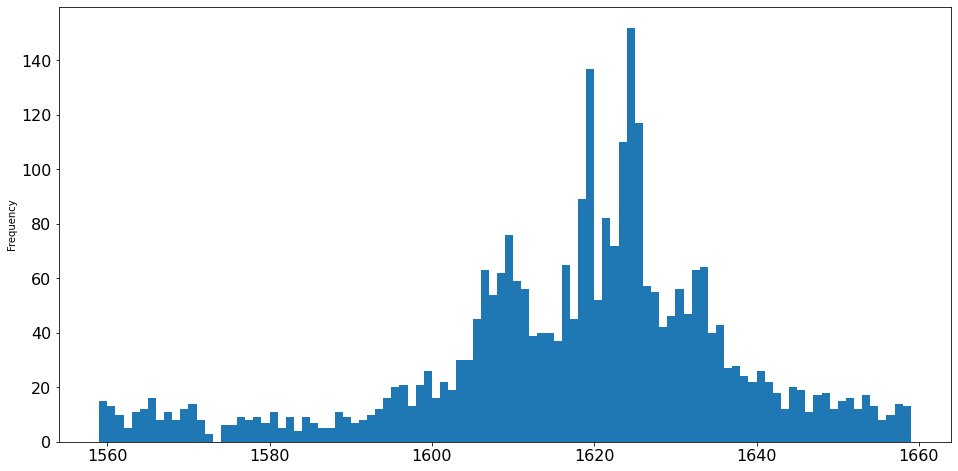
\includegraphics[scale=0.4]{graph/Distribution of the Publication Year.png}
\caption{Distribution of the Publication Year}
\label{fig:pubYear}
\end{figure}

\begin{figure}[H]
\centering
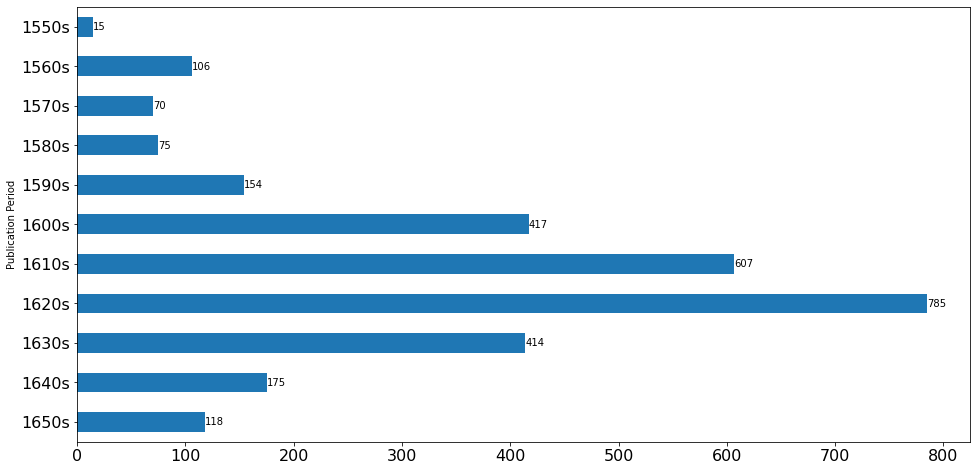
\includegraphics[scale=0.4]{graph/Distribution of the Publication Year (in Decade Level).png}
\caption{Distribution of the Publication Year (in decade level)}
\label{fig:pubDecade}
\end{figure}

\subsection*{Role}
1220 (36.42\%) people had been an author, which is the most common role people hold in this dataset. However, if we compute the average number of publications a role involved, we can find that if a person were a printer/publisher, this person would participate in an average of 29.15 publications, significantly more than the overall average (3.49), showing that the printer/publisher might be the most influential role of the Douai publishing industry.

\begin{figure}[H]
\centering
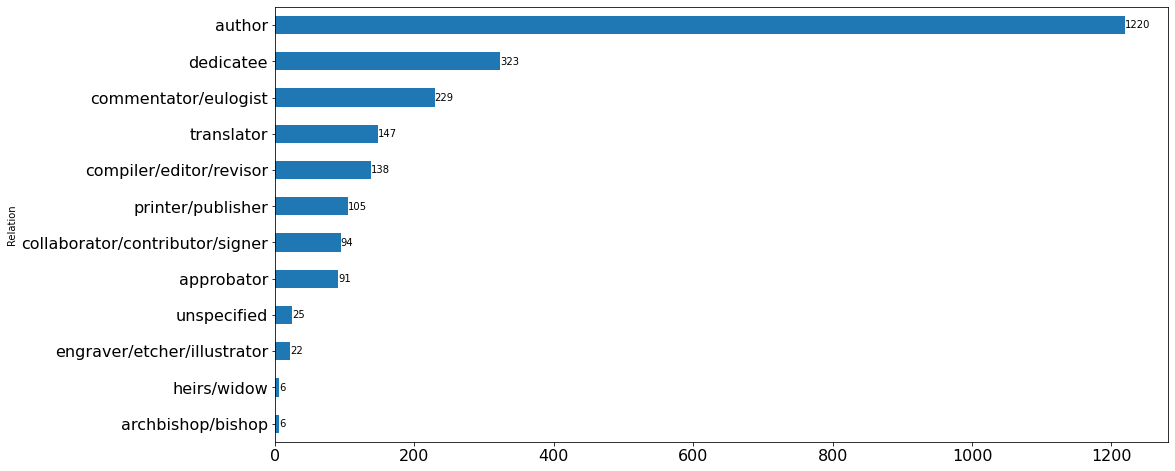
\includegraphics[scale=0.36]{graph/Distribution of Roles (in Person Level).png}
\caption{Distribution of Roles}
\label{fig:distRole}
\end{figure}

\subsection*{Place of Birth and Death}
There are 261 birth places and 122 death places mentioned in this dataset. Since this is a dataset about Douai, it is obvious that there were most people born or died around there. A remarkable aspect is that Antwerp is in second place among the birth places, but not even in the top 5 among the death places, reflecting the history that Antwerp was a renowned printing centre within the Low Countries but eventually lots of people in the industry moved from there to Douai (Soetaert, 2019a, 2014; Soetaert \& Wyffels, 2021). Although scholars (Soetaert, 2019a, 2014; Soetaert \& Wyffels, 2021) also observe the mobility from Leuven, the trend is not as obvious as Antwerp in this dataset. The difference between Antwerp and Leuven was the development of a university, which can be a reason that the moving trend from Leuven is not as evident as from Antwerp.

\begin{table}[H]
\centering
\caption{Top 5 Birth and Death Places}
\label{tab:top5BD}
\begin{tabular}{l|c|l|c}
\multicolumn{1}{c|}{\textbf{Top 5 Birth Places}} & \multicolumn{1}{c|}{\textbf{Count}} & \multicolumn{1}{c|}{\textbf{Top 5 Death Places}} & \multicolumn{1}{c}{\textbf{Count}} \\ \hline
Douai                                            & 20                                  & Douai                                            & 60                                 \\
Lille                                            & 12                                  & Roma                                             & 28                                 \\
Antwerpen                                        & 12                                  & Lille                                            & 17                                 \\
Leuven                                           & 9                                   & Tournai                                          & 17                                 \\
Tournai                                          & 9                                   & Leuven                                           & 17                                
\end{tabular}
\end{table}

For countries, there are 15 countries mentioned. A pivotal observation is that if we compute the proportion of the count of Britain within the birth countries (13.65\%) and its proportion within the death countries (5.6\%), and conduct the proportional z-test\footnote{To see if the proportion of two groups have a significant difference (Freedman et al., 2007).} between them, it shows a significant difference (z score = 3.82, p-value = $0.00013 < 0.05$), indicating the historical trend that English Catholics were escaping from their homeland due to the English Reformation (Soetaert, 2019a, 2014; Soetaert \& Soen, 2020a; Soetaert \& Wyffels, 2021).

\begin{figure}[H]
\centering
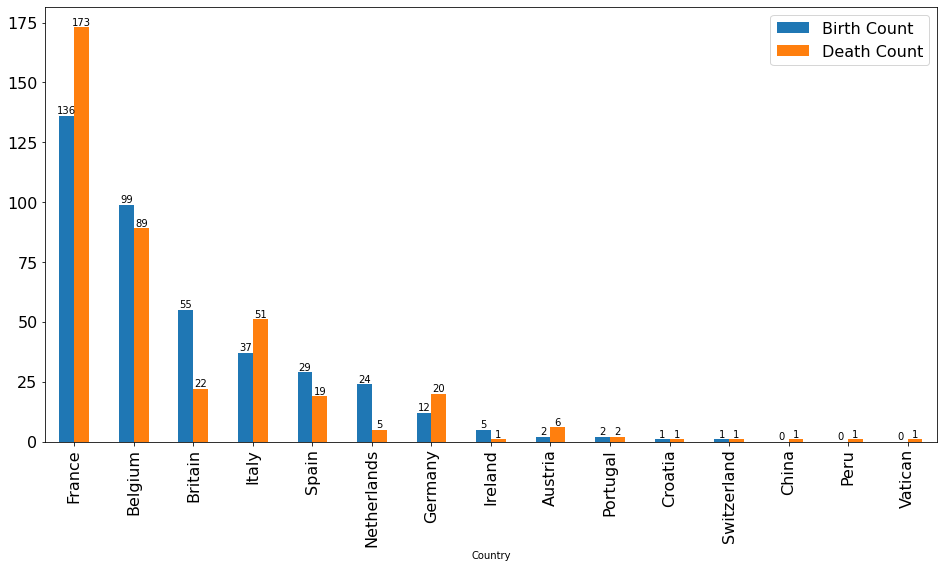
\includegraphics[scale=0.4]{graph/Count of Birth and Death Country.png}
\caption{Count of Birth and Death Country}
\label{fig:countCountry}
\end{figure}

\pagebreak
Nevertheless, the countries tagged to each place in this dataset seem to be according to the border nowadays instead of the border in early modern Europe. For example, in Table \ref{tab:extractPlace}, “Douai” is tagged with “FR” (France), which is not historically accurate since Douai belonged to Low Countries during 1559-1659 (Soen, 2016; Soetaert \& Soen, 2020a). Although computing metrics of Britain may not be a problem since its border is almost the same as today, it may lead to errors when analysing within the European continent. Therefore, the country labels for each place need to be adjusted and it will be done in Chapter \ref{comeAndGo}.

Another issue is that only 403 people’s birth places (19.37\%) and 393 people’s death places (18.89\%) are recorded in this dataset. Although these numbers of records (all $> 30$) can be considered a large sample size to infer the population (Kwak \& Kim, 2017), it should be kept in mind that when using the information of people’s birth and death places in this research, the results are inferential.

\counterwithout{footnote}{chapter}
\chapter{Exploiting Social Network Analysis}
\label{SNA}
Social Network Analysis is the main research method of this paper. This chapter provides general instruction on how Social Network Analysis is conducted and explains the metrics and tools that are applied in the later chapters.

Social Network analysis is a quantitative method to study the interactions between people (Carrington \& Scott, 2011; Wasserman \& Faust, 1994), and the key concept of it is a Network. A Network consists of nodes and edges, a node is an entity, and an edge is a connection between the two entities. For example, if we want to build the Network of an office, we can make each node a member of the office, and an edge can be a project that two members are working on together.

\begin{figure}[H]
\centering
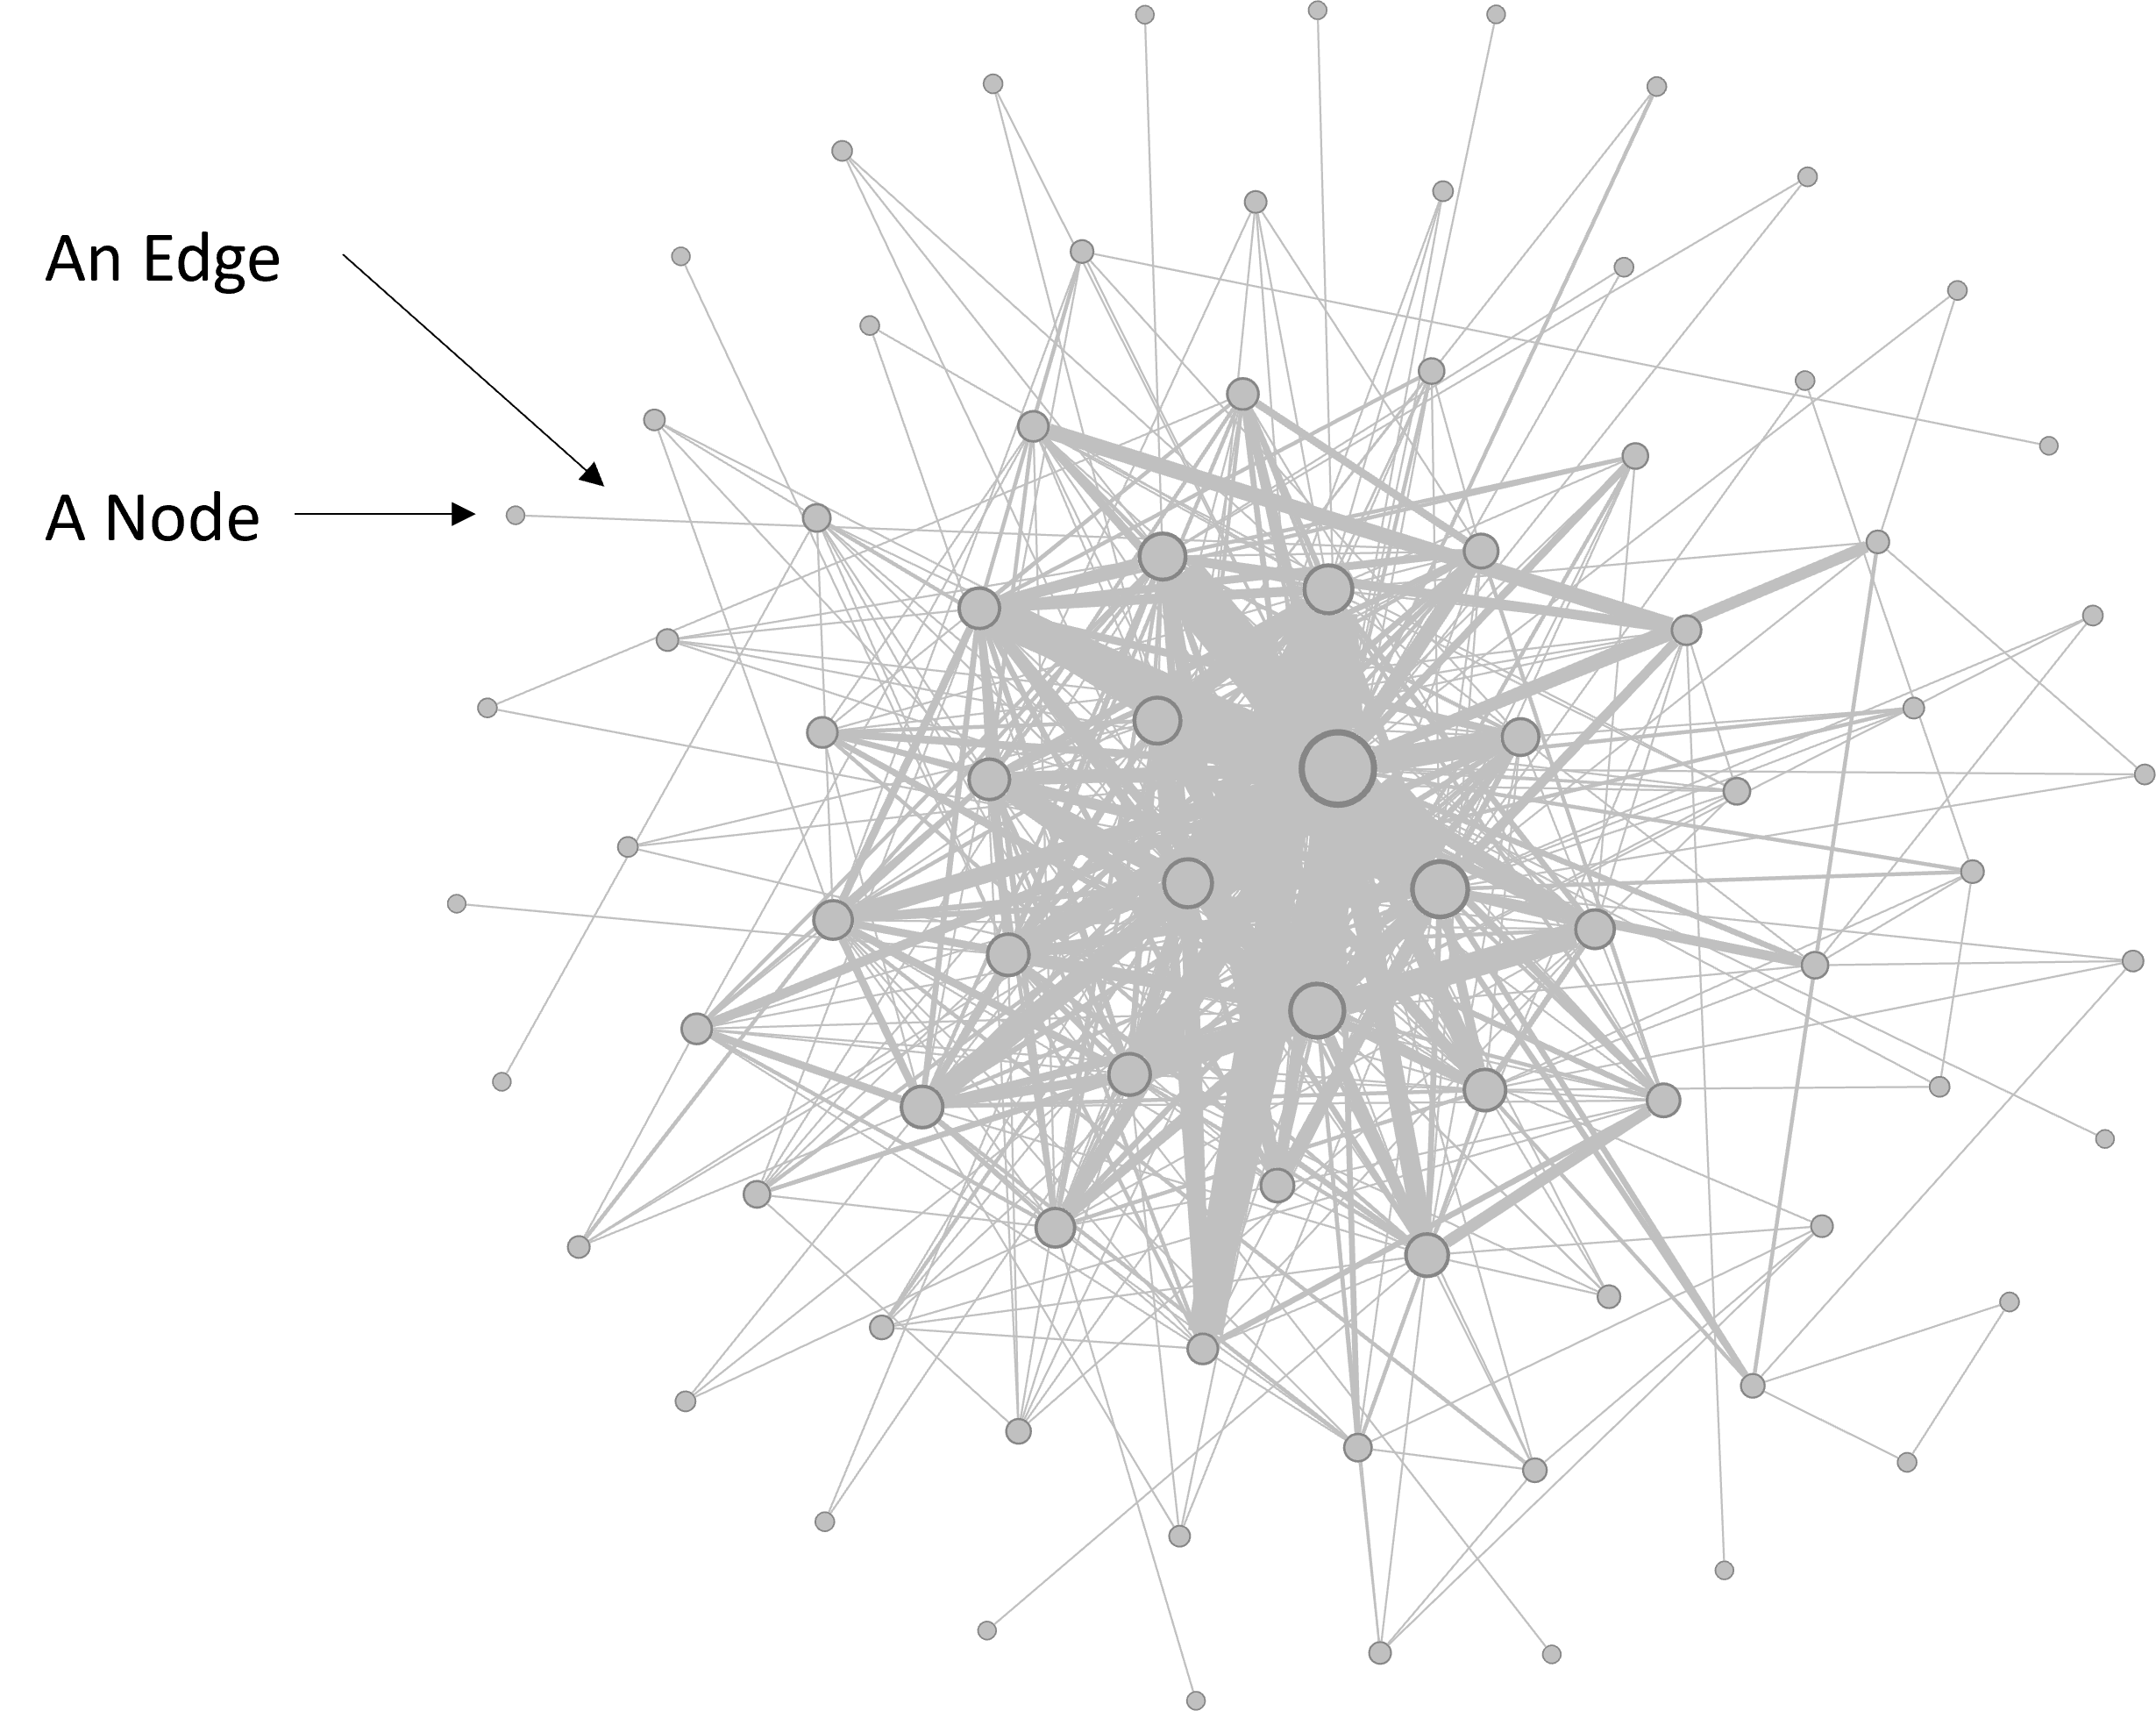
\includegraphics[scale=0.7]{graph/network explain.png}
\caption{An Example of a Social Network}
\label{fig:networkExplain}
\end{figure}

\pagebreak
Several metrics (Carrington \& Scott, 2011; Wasserman \& Faust, 1994) are conducted to gain a deeper understanding of the Networks we are investigating:
\\

\textbf{Degree and Degree Centrality:} a Degree of a node represents how many nodes this node is connected to. For example, if a member in the office has a Degree of 5, it means that he is working with five other members. Degree Centrality normalises the Degree, so having a Degree of 5 in an office that has 21 members will get you a Degree Centrality of 5/(21-1) = 0.25.

\textbf{Betweenness Centrality:} it quantifies the number of times a node lies within the shortest paths between pairs of other nodes. In our office example, having a higher Betweenness Centrality means that the member serves well as a bridge, facilitating connections between other members.

\textbf{Closeness Centrality:} it measures how close a node is to all other nodes in a Network. Nodes with high Closeness Centrality have shorter average distances to other nodes, highlighting how well a node is connected to the entire Network.

\textbf{Clustering Coefficient:} it computes the extent to which the neighbours of a node are interconnected. A higher Clustering Coefficient suggests that the node's neighbours are more likely to form a subgroup or cluster within the Network.

\textbf{Density:} it calculates the ratio of the actual number of edges in a Network to the total number of possible edges. This measure indicates how well-connected the Network is. For example, in a Network with 5 nodes, there can be 10 possible edges in total. If this Network has 6 actual edges, its density would be calculated as 6/10 = 0.6.

\textbf{Eigenvector Centrality:} it considers not only how well a node is connected to others but also the Centrality of those nodes. A node having a higher Eigenvector Centrality has the potential to be influential to the Network.

\textbf{Modularity and Modularity Class:} it determines how well a Network can be divided into distinct groups. If a Network of an office has a high Modularity, it implies the presence of meaningful subgroups in this office. Modularity Class, on the other hand, is the outcome of an algorithm that assigns nodes to these meaningful groups.
\\

In addition, several tools are applied to visualise and compute our Networks:
\\

\textbf{nodegoat:}\footnote{\url{https://nodegoat.net/about}} a web-based tool to project your Network on a map, which allows you to observe the mobility of your Network. Network graphs in Chapter \ref{comeAndGo} are created by this tool.

\textbf{Gephi:}\footnote{\url{https://gephi.org/features/}} a commonly used software to plot the Network you have built. Network graphs in Chapters \ref{languages}, \ref{influencers} and \ref{differentNetwork} are drawn by this software.

\textbf{NetworkX:}\footnote{\url{https://Networkx.org/}} a Python package to fast calculate metrics of your Network. The calculation in Chapters \ref{comeAndGo}, \ref{languages}, \ref{influencers} and \ref{differentNetwork} are done with the help of this package.

\textbf{Retina:}\footnote{\url{https://ouestware.gitlab.io/retina/1.0.0-beta.1/}} a web-based tool that you can upload the GEXF or GraphML file of your Network and share it as an interactive dashboard. Networks in Chapter \ref{languages} and Chapter \ref{differentNetwork}.2 are shared with this tool.

\counterwithout{footnote}{chapter}
\chapter{Coming and Going of the People}
\label{comeAndGo}
The development of the publishing industry in the ecclesiastical province of Cambrai was strongly related to the coming of the English Catholics (Soetaert, 2019a, 2014; Soetaert \& Soen, 2020a). The strongest force that triggered the movement of English Catholics could be the persecution from the English ruling class. The tension between the Catholics and the Protestants in England started with the establishment of the Church of England in the late 16th century which broke England with Rome, the Catholic authority (McCoog, 2001). The succession of Queen Elizabeth I (1558), who was a supporter of Protestants, marked the rising of a period of anti-Catholicism in England (Bossy, 1962; Hibbard, 1980). During this “Early Stuart Period” (until the “Stuart Restoration” in 1660), English Catholics could be considered refugees and they were seeking other places to continue the development of the English Catholic church (Bossy, 1962). Thanks to the establishment of the University of Douai (1559) which drove the development of Catholic and English-related institutions, Douai became a preferred place for English Catholics for publishing Catholic publications (Boureau et al., 1989; Soetaert, 2019a, 2014; Soetaert \& Soen, 2020a; Soetaert \& Wyffels, 2021).

It can be interesting to recreate the mobility of this immigration. However, since this dataset only records the birth and death place of a person, we use this information as a proxy. Specifically, the birth place is assumed where a person came from, and the death place is considered where a person ended up going. With this assumption, we investigate that does this dataset reflects the trend of the immigration from Britain (Soetaert, 2019a, 2014; Soetaert \& Soen, 2020a; Soetaert \& Wyffels, 2021), and where could be the next place that had a promising future for the publishing industry since more people ended up going there.

However, as mentioned in Chapter \ref{Duacensia}, since there are only about 20\% of people’s birth and death places recorded in this dataset, the results of this chapter show not an accurate whole picture but a rough estimate of the mobility of people in the Douai publishing industry.

\pagebreak
\section{Adjusting the Country Label}
As mentioned in Chapter \ref{Duacensia}, current labels of countries to each (birth and death) place are not historically accurate. By consulting several old maps (‘Map of Europe, 1648’, n.d.; Mercator et al., 1623a, 1623b; Sanson, 1648) and references (De Ridder et al., 2020; Soen, 2016; Soen et al., 2019; Soen \& Junot, 2021), all mentioned places in this dataset are retagged with a more historical accurately region.

The biggest challenge is the difference between the border of France then (1559-1659) and nowadays. Some places that are marked as “FR”, such as Douai, Saint-Omer, and Lille, belonged to Low Countries during our research period. From our reference mentioned above, in this dataset, “Hesdin” and “Stenay” were the southeast part of the Low Countries. We draw a line of the connection of these two places as an anchor to mark all the places above this line with the region label “Low Countries”. Figure \ref{fig:cateLow}\footnote{It is important to know that this is not the actual border that distinguished the France and Low Countries during this period. Rather, this is just the two places in this dataset that is the closest to the border so they can be used for our categorisation.} illustrates the anchor to separate the regions of France and the Low Countries, and places within the grey area are tagged as in the Low Countries Region. Table \ref{tab:conAdjust} provides some examples of the adjusted labels.

\begin{figure}[H]
\centering
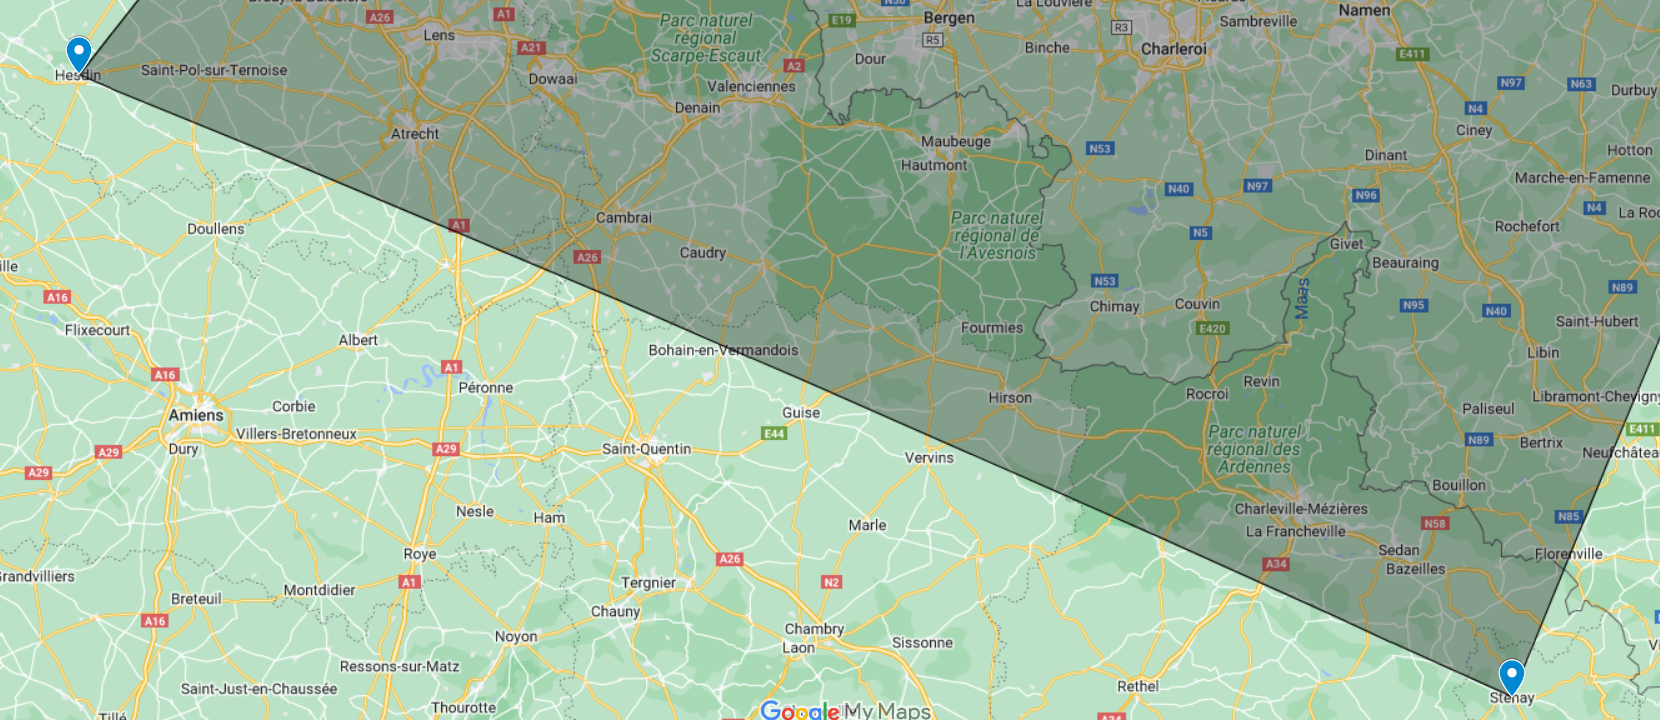
\includegraphics[scale=0.4]{graph/Categorising Low Countries.png}
\caption{Categorising Low Countries}
\label{fig:cateLow}
\end{figure}

\begin{table}[H]
\centering
\caption{Examples of Country Adjustment}
\label{tab:conAdjust}
\begin{tabular}{lll}
\multicolumn{1}{c}{\textbf{Place}} & \multicolumn{1}{c}{\textbf{Original Country Label}} & \multicolumn{1}{c}{\textbf{Adjusted Region Label}} \\ \hline
Kortrijk                           & BE                                                  & Low Countries                                      \\
Douai                              & FR                                                  & Low Countries                                      \\
Saint-Omer                         & FR                                                  & Low Countries                                      \\
Tournai                            & BE                                                  & Low Countries                                     
\end{tabular}
\end{table}

In the end, places are re-categorised into 9 regions. Table \ref{tab:infoRegion} provides backgrounds of some regions used to categorise places that were quite different from today and Figure \ref{fig:countBDRegion} shows the distribution of regions people in this dataset were born and dead.

\begin{table}[H]
\centering
\caption{Backgrounds of Some Regions}
\label{tab:infoRegion}
\begin{tabularx}{\textwidth}{l|X}
\multicolumn{1}{c|}{\textbf{Region}} & \multicolumn{1}{c}{\textbf{Note}}                                                                                                                                                                                          \\ \hline
Britain                              & Includes places in England, Scotland, Wales, and Ireland.                                                                                                                                                                  \\
China                                &                                                                                                                                                                                                                            \\
France                               &                                                                                                                                                                                                                            \\
Genève                               & Genève (Republic of Genève) was an independent city-state from 1541 to 1798 (Church \& Head, 2013).                                                                                                                        \\
Holy Roman Empire                    & Includes places that are in Germany and Austria nowadays.                                                                                                                                                                  \\
Iberian Union                        & From 1580 to 1640, Felipe II united Spain and Portugal (LAURA FERNÁNDEZ-GONZÁLEZ, 2021).                                                                                                                                   \\
Italy                                & It was not a country in the early modern era but a combination of several independent city-states (Duggan, 2014).                                                                                                          \\
Low Countries                        & Places located in the Dutch Republic (1581-1795) and the Spanish (Habsburg) Netherlands (1556-1714) could be considered within Low Countries (De Ridder et al., 2020; Soen, 2015; Soen et al., 2019; Soen \& Junot, 2021). \\
Peru                                 &                                                                                                                                                                                                                           
\end{tabularx}
\end{table}

\begin{figure}[H]
\centering
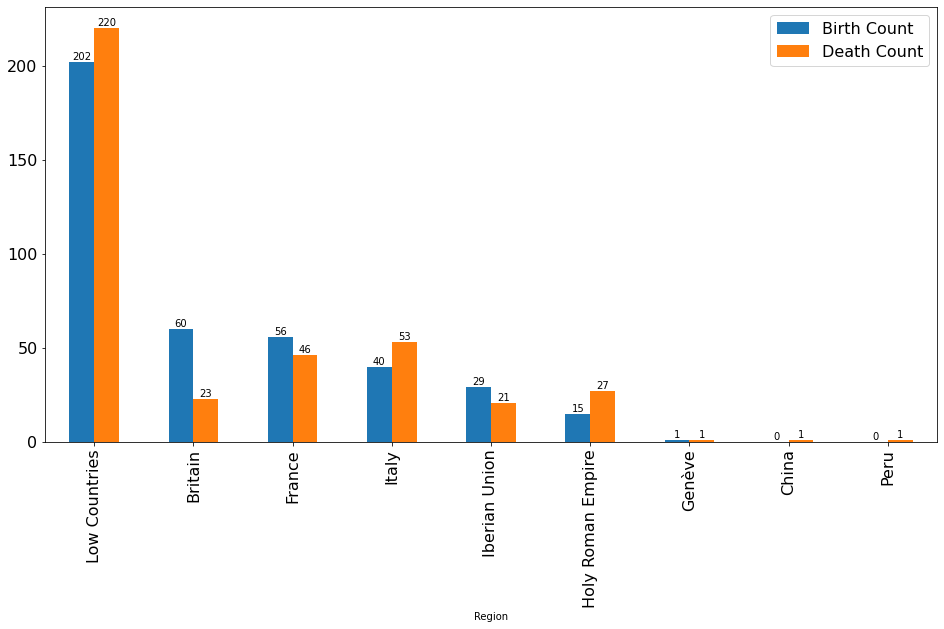
\includegraphics[scale=0.4]{graph/Count of Birth and Death Region.png}
\caption{Distribution of Birth and Death Region}
\label{fig:countBDRegion}
\end{figure}

\pagebreak
\section{Building the Network}
The nodes of the Network in this chapter are all the distinct places of birth and death mentioned in this dataset, and there are 333 nodes in total. All the nodes (places) are tagged with the categorised region label from the previous section.

The edges of this Network are the directed connections between the birth and death places. For example (Figure \ref{fig:examplePlaceNet}), if there is a person that was born in Leuven and died in Douai, there will be a directed edge from Leuven to Douai in the Network. In total, there are 333 edges, and because of the situations that 1) some records of a person only have either this person’s birth or death place, and 2) some people were born and died at the same place, there are 64 nodes that do not have an edge.

\begin{figure}[H]
\centering
\includesvg[scale=1.2]{graph/An Example of Edge in Place Network.svg}
\caption{An Example of Edge in the Place Network}
\label{fig:examplePlaceNet}
\end{figure}

\section{Findings}
With the help of the web-based tool, nodegoat, we can project the whole Place Network on a map (Figure \ref{fig:placeNet}). Each edge (the green line) represents a person’s life journey, the blue node is where this person was from (birth place), and the red node is where this person ended up going (death place). The size of the node illustrates the Degree of the place, the bigger the size, the higher the Degree it has. The Degree here indicates the number of edges a node has. In other words, if a place has a high Degree, it is a popular place people originated from or are destinated to.

You can observe immediately that there are two interesting edges connected outside Europe (Figure \ref{fig:toPandC}). The one that went to Peru was Juan de Atienza, a Spanish Jesuit missionary who was made Provincial of the Jesuits in Peru in 1580 (Herbermann, 1913). The other one who went to China was Nicolas Trigault, a Jesuit who originated from Douai. He was sent to East Asia for missionary work and ended up settling down in Hangzhou, China (Mungello, 1985)

\begin{figure}[H]
\centering
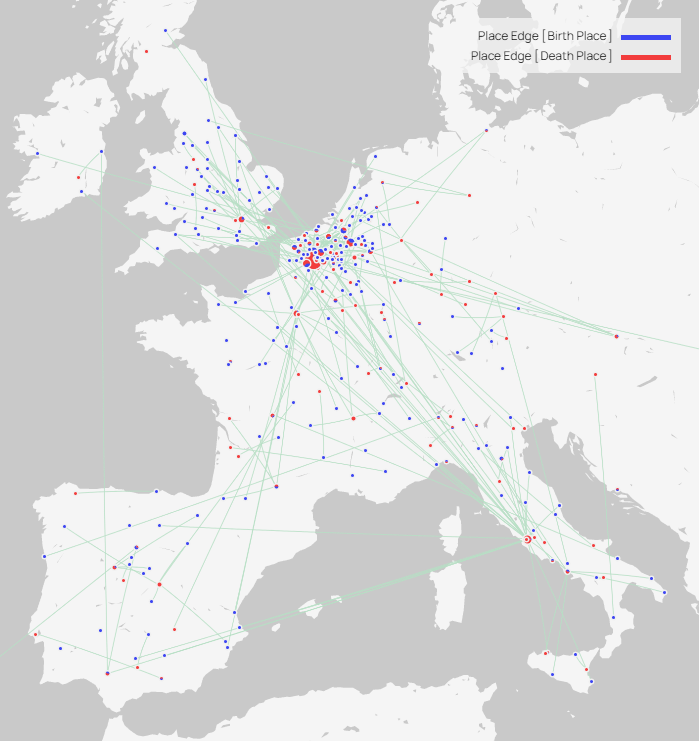
\includegraphics[scale=0.7]{graph/Place Network.png}
\caption{The Place Network}
\label{fig:placeNet}
\end{figure}

\begin{figure}[H]
\centering
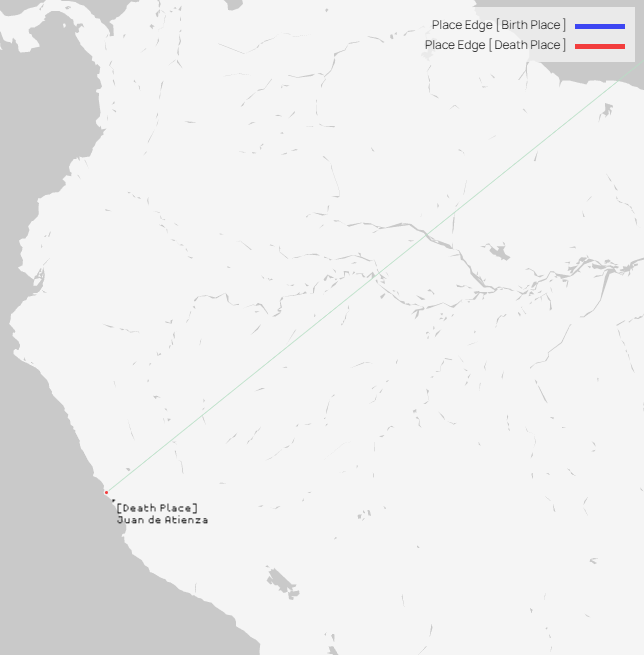
\includegraphics[scale=0.4]{graph/Edge to Peru.png}
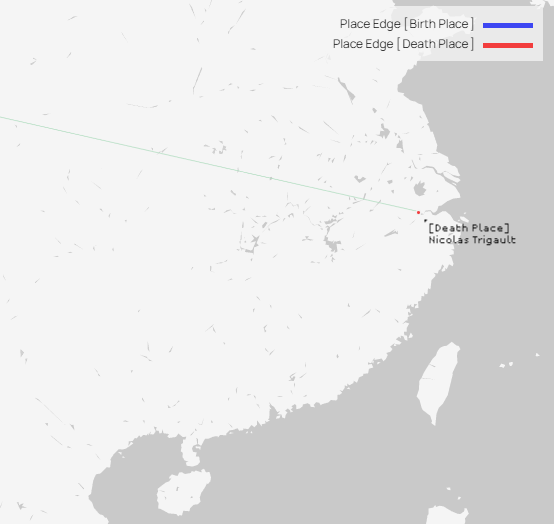
\includegraphics[scale=0.5]{graph/Edge to China.png}
\caption{The Edge Connected to Peru (left) and China (right)}
\label{fig:toPandC}
\end{figure}

\pagebreak
Since the analysis of this chapter is to see the mobility of people, we look at the InDegree and OutDegree of each place separately instead of its overall Degree. InDegree indicates the number of edges directed to the node. In other words, if a place has a higher InDegree, it can be a popular final stop for the people in the industry. On the contrary, OutDegree shows the number of edges directed from the node, implicating the ethnic composition of the industry.

Looking at the Network graph around Britain (Figure \ref{fig:britNet}), you can notice that there are more blue nodes (people’s hometowns) on the island than red nodes (people’s destinations). In general, most of the connecting direction of the blue nodes is pointing overseas, showing the trend of mobility from Britain. Since this is a dataset about Douai, it is obvious that the destination of these Britain blue nodes is directed to places around Douai. Furthermore, the difference between the mean of InDegree and OutDegree within Britain is bigger than in other regions, and the difference reaches statistical significance in the t-test\footnote{To see if the mean of two groups have a significant difference (Freedman et al., 2007).} (t = -2.78, p = $0.0006 < 0.05$). The result implies that for the people in the publishing industry in Douai, Britain was the place they tended more to come from instead of going to, and this tendency did not show in other regions. The two observations can be evidence of the history that English Catholics were escaping from their homeland, and the ecclesiastical province of Cambrai could be an important destination for them during this period (Boureau et al., 1989; Soetaert, 2019a, 2014; Soetaert \& Soen, 2020a; Soetaert \& Wyffels, 2021).

\begin{figure}[H]
\centering
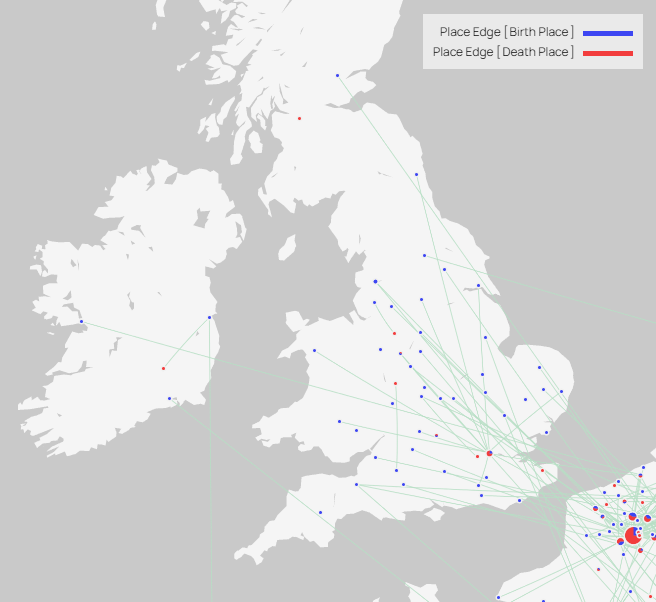
\includegraphics[scale=0.7]{graph/Place Network (Britain).png}
\caption{The Place Network around Britain}
\label{fig:britNet}
\end{figure}

\begin{table}[H]
\centering
\caption{Mean of InDegree and OutDegree of Each Region}
\label{tab:inOutMean}
\begin{tabular}{lcccc}
\multicolumn{1}{l|}{}                  & \textbf{}                         & \textbf{InDegree (Death)}          & \textbf{}                         & \textbf{OutDegree (Birth)}  \\ \hline
\multicolumn{1}{c|}{\textbf{Region}}   & \multicolumn{1}{c|}{\textbf{n}\tablefootnote{Number of birth places in this region.}}   & \multicolumn{1}{c|}{\textbf{Mean}} & \multicolumn{1}{c|}{\textbf{n}\tablefootnote{Number of death places in this region.}}   & \textbf{Mean}               \\ \hline
\multicolumn{1}{l|}{Low Countries}     & \multicolumn{1}{c|}{\textit{220}} & \multicolumn{1}{c|}{1.61}          & \multicolumn{1}{c|}{\textit{202}} & 1.51                        \\
\multicolumn{1}{l|}{France}            & \multicolumn{1}{c|}{\textit{46}}  & \multicolumn{1}{c|}{0.75}          & \multicolumn{1}{c|}{\textit{56}}  & 0.92                        \\
\multicolumn{1}{l|}{Italy}             & \multicolumn{1}{c|}{\textit{53}}  & \multicolumn{1}{c|}{1.07}          & \multicolumn{1}{c|}{\textit{40}}  & 0.87                        \\
\multicolumn{1}{l|}{Britain}           & \multicolumn{1}{c|}{\textit{23}}  & \multicolumn{1}{c|}{0.36}          & \multicolumn{1}{c|}{\textit{60}}  & {\color[HTML]{CB0000} 0.98} \\
\multicolumn{1}{l|}{Iberian Union}     & \multicolumn{1}{c|}{\textit{21}}  & \multicolumn{1}{c|}{0.72}          & \multicolumn{1}{c|}{\textit{29}}  & 1.00                        \\
\multicolumn{1}{l|}{Holy Roman Empire\tablefootnote{The difference of the mean of InDegree and OutDegree at Holy Roman Empire is also big. Although not achieving statistical significance, it does show an interesting trend that worth investigating further in the future.}} & \multicolumn{1}{c|}{\textit{27}}  & \multicolumn{1}{c|}{1.00}          & \multicolumn{1}{c|}{\textit{15}}  & 0.56                        \\
\multicolumn{1}{l|}{Genève}            & \multicolumn{1}{c|}{\textit{1}}   & \multicolumn{1}{c|}{0.50}          & \multicolumn{1}{c|}{\textit{1}}   & 0.50                        \\
\multicolumn{1}{l|}{China}             & \multicolumn{1}{c|}{\textit{0}}   & \multicolumn{1}{c|}{1.00}          & \multicolumn{1}{c|}{\textit{1}}   & 0.00                        \\
\multicolumn{1}{l|}{Peru}              & \multicolumn{1}{c|}{\textit{0}}   & \multicolumn{1}{c|}{1.00}          & \multicolumn{1}{c|}{\textit{1}}   & 0.00                        \\ \hline
\multicolumn{5}{l}{* {\color[HTML]{CB0000} Red numbers} are significantly higher than the other degree of this region.}                                                                            
\end{tabular}
\end{table}

Now look at the Degrees of each place (Table \ref{tab:top5IndOut}). In general, the OutDegrees of places are lower than their InDegrees, showing that where people in the Douai publishing industry were from was more spread around than where people settled down, confirming the historical statement that Douai attracted diverse people from all over Europe involved in publishing (Soetaert, 2019a, 2014; Soetaert \& Wyffels, 2021). Antwerp has the highest OutDegree, indicating that people were moving away from there more, which not only demonstrates the decline of its publishing industry in the 1570s (Soetaert, 2019a) but also presents the importance of having a university could be beneficial for the industry because Antwerp did not have one at that time but places that have a higher InDegree, such as Douai (University of Douai), Leuven (University of Louvain) and Paris (University of Paris) (Goeing et al., 2021), did.

Table \ref{tab:top5IndOut} and left of Figure \ref{fig:aroundCandR} show that places around the ecclesiastical province of Cambrai have a higher Degree, revealing that most of the people in this dataset moved within this area. Nonetheless, Rome (right of Figure \ref{fig:aroundCandR}), which is far away from the Cambrai province, has the second highest InDegree (Table \ref{tab:top5IndOut}), marking this rising centre in publishing in early modern Europe (Jones et al., 2019) started attracting people from other publishing centres.

\begin{table}[H]
\centering
\caption{Top 5 InDegree and OutDegree of Places}
\label{tab:top5IndOut}
\begin{tabular}{lclc}
\multicolumn{2}{c|}{\textbf{Top 5 InDegree (Death)}}                                                 & \multicolumn{2}{c}{\textbf{Top 5 OutDegree (Birth)}}                                \\ \hline
\multicolumn{1}{l|}{{\color[HTML]{303498} Douai}}   & \multicolumn{1}{c|}{{\color[HTML]{303498} 37}} & \multicolumn{1}{l|}{Antwerpen}                           & 9                        \\
\multicolumn{1}{l|}{Roma}                           & \multicolumn{1}{c|}{24}                        & \multicolumn{1}{l|}{{\color[HTML]{303498} Douai}}        & {\color[HTML]{303498} 8} \\
\multicolumn{1}{l|}{Leuven}                         & \multicolumn{1}{c|}{16}                        & \multicolumn{1}{l|}{{\color[HTML]{303498} Lille}}        & {\color[HTML]{303498} 8} \\
\multicolumn{1}{l|}{Paris}                          & \multicolumn{1}{c|}{15}                        & \multicolumn{1}{l|}{{\color[HTML]{303498} Arras}}        & {\color[HTML]{303498} 6} \\
\multicolumn{1}{l|}{{\color[HTML]{303498} Tournai}} & \multicolumn{1}{c|}{{\color[HTML]{303498} 14}} & \multicolumn{1}{l|}{{\color[HTML]{303498} Valenciennes}} & {\color[HTML]{303498} 5} \\ \hline
\multicolumn{4}{l}{* {\color[HTML]{303498} Blue places} are within the ecclesiastical province of Cambrai.}                                                                                                       
\end{tabular}
\end{table}

\begin{figure}[H]
\centering
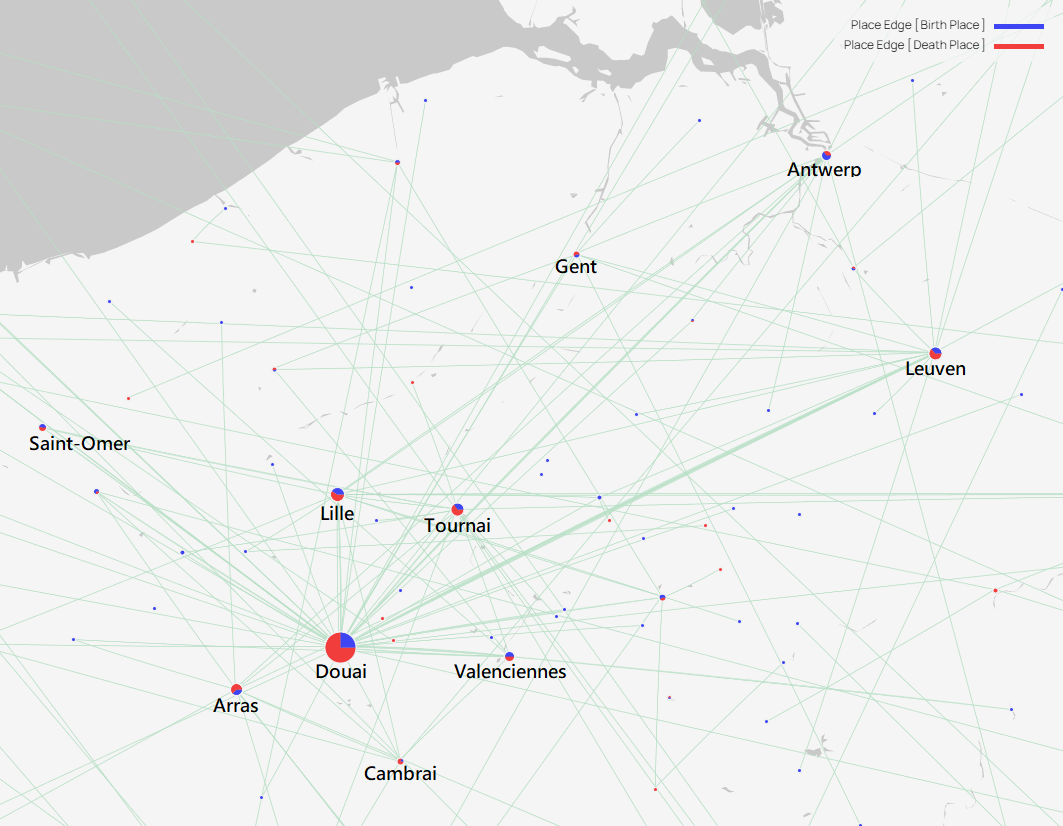
\includegraphics[scale=0.45]{graph/Cambrai_annotated.png}
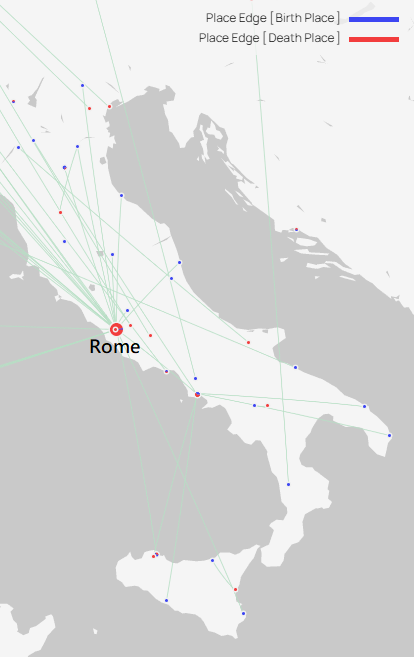
\includegraphics[scale=0.58]{graph/Rome_annotated.png}
\caption{Place Network around the province of Cambrai (left) and Rome (right)}
\label{fig:aroundCandR}
\end{figure}

\counterwithout{footnote}{chapter}
\chapter{English Catholics and the Industry}
\label{languages}
The previous chapter illustrates the trend of English Catholics moving to the ecclesiastical province of Cambrai, especially Douai. But how did they participate in the process of the development of the publishing industry in Douai? With the Network of people involved, this chapter describes the phases of growth and decline of the industry and portrays the impact of English Catholics on the industry through time.

As mentioned in Chapter \ref{Duacensia}, there are only about 20\% records of where people were from in this dataset, which can be enough for estimation but may not be sufficient to depict the dynamic of the Network in the industry. Since where a person was from could affect the languages of publications this person would involve in (Soen et al., 2015; Soetaert, 2019a, 2014; Soetaert \& Soen, 2020a; Soetaert \& Wyffels, 2021), in this chapter, the language of each publication is considered a proxy of the involved people’s origin or nationality to construct their interactions with people from other origin or nationality in the Network.

\section{Adding the Language Label}
Since the language of publications is not provided in the dataset, we use the title of the publication to represent the language of the publication. Open-source Python libraries “langdetect”\footnote{https://pypi.org/project/langdetect/} and “lingua-py”\footnote{https://github.com/pemistahl/lingua-py} are applied to identify the language\footnote{The reason that there are two libraries applied is that after the first application of “lingua-py”, we found that it could detect Latin well but not English. Therefore, “langdetect” is also applied on the publications other than in Latin.} of the titles. Figure \ref{fig:distLan} shows that the top 2 used languages of publications published in Douai were Latin (2036, 69.34\%) and French (673, 22.92\%). It is no surprise that there are more Latin publications since the theme of this dataset is religious books and Latin was the main language for Catholics (Soen et al., 2015). In addition, French being the main vernacular of the Cambrai region during this period (Soetaert, 2014) explains why there are also a lot of French publications.

\begin{figure}[H]
\centering
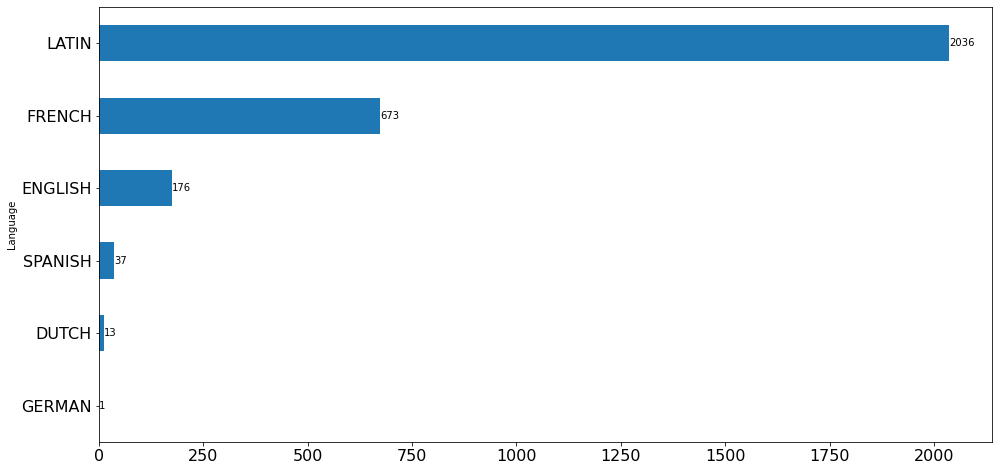
\includegraphics[scale=0.4]{graph/Distribution of Languages.png}
\caption{Distribution of Languages}
\label{fig:distLan}
\end{figure}

If we look at the proportion of languages that people from each region had involved, it does align with the statement that people’s backgrounds were related to the languages they participated in (Soen et al., 2015; Soetaert, 2019a, 2014; Soetaert \& Soen, 2020a; Soetaert \& Wyffels, 2021). Figure \ref{fig:stackLan}\footnote{Since people can participate in several languages, the sum of each proportion is not exactly 1.0.} shows that people from Britain tended to involve in English publications more than people from other regions, and so did people from France to French publications and people from Iberian Union to Spanish publications. This tendency reaches statistical significance (p-value $< 0.05$ in z-test) (Table \ref{tab:crossRegionLan}). Nonetheless, for the French language, people from regions other than Britain also participated a lot in French publications. Since French was the predominant language in Douai (Soen et al., 2015; Soetaert, 2019a, 2014; Soetaert \& Soen, 2020a), its dynamic should not only be considered the activities of people from France but also the local needs; for Spanish, since there were only 37 (1.26\%) publications in this language, the quantity can be not big enough to portray the activities of people from the Iberian Union.

In addition, the result of the z-test also shows that people from the Low Countries tended to participate more in Latin publications. However, it is important to consider that Douai was in the Low Countries. Therefore, the results may simply indicate that there was a significant business need for Latin publications in this region, and local people were highly involved in meeting that demand, rather than suggesting that people from the Low Countries were culturally more inclined towards the Latin language.

As a result, we can only treat the dynamic of English publications in the Network as the activities of people from Britain, and they most likely were English Catholics.

\begin{figure}[H]
\centering
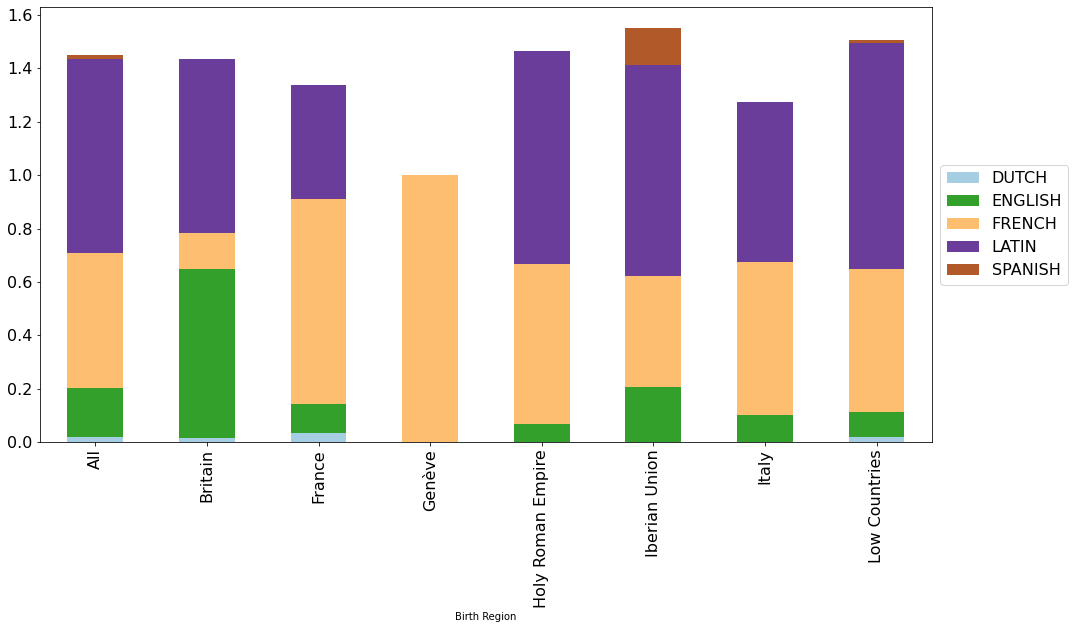
\includegraphics[scale=0.4]{graph/Stack Chart of Birth Region and Language.png}
\caption{Stack Chart of Birth Region and Language}
\label{fig:stackLan}
\end{figure}

\begin{table}[H]
\centering
\caption{Cross Table of Birth Region and Language (in proportion)}
\label{tab:crossRegionLan}
\begin{tabular}{lccccccc}
\multicolumn{1}{l|}{}           & \textbf{Britain}            & \textbf{France}             & \textbf{Genève} & \textbf{Holy} & \textbf{Iberian}            & \textbf{Italy} & \textbf{Low}                \\ \hline
\multicolumn{1}{l|}{\textit{n\tablefootnote{Number of people from each region.}}} & \textit{60}                 & \textit{56}                 & \textit{1}      & \textit{15}   & \textit{29}                 & \textit{40}    & \textit{202}                \\ \hline
\multicolumn{1}{l|}{Dutch}      & 0.02                        & 0.04                        & 0.00            & 0.00          & 0.00                        & 0.00           & 0.02                        \\
\multicolumn{1}{l|}{English}    & {\color[HTML]{CB0000} 0.63} & 0.11                        & 0.00            & 0.07          & 0.21                        & 0.10           & 0.09                        \\
\multicolumn{1}{l|}{French}     & 0.13                        & {\color[HTML]{CB0000} 0.77} & 1.00            & 0.60          & 0.41                        & 0.57           & 0.53                        \\
\multicolumn{1}{l|}{Latin}      & 0.65                        & 0.43                        & 0.00            & 0.80          & 0.79                        & 0.60           & {\color[HTML]{CB0000} 0.85} \\
\multicolumn{1}{l|}{Spanish}    & 0.00                        & 0.00                        & 0.00            & 0.00          & {\color[HTML]{CB0000} 0.14} & 0.00           & 0.01                        \\ \hline
\multicolumn{8}{l}{* {\color[HTML]{CB0000} Red numbers} are significantly higher than other groups.\tablefootnote{By proportional z-test. Britain vs. non-Britain in English: z=9.75, p=1.80e-22; France vs. non-France in French: z=4.22, p=2.44e-5; Iberian Union vs. non- Iberian Union in Spanish: z=5.68, p=1.35e-8; Low Countries vs. non-Low Countries in Latin: z=5.40, p=6.74e-8.}}                                                                                                                   
\end{tabular}
\end{table}

\section{Building the Network}
The Network is built based on the people involved in the same publication. Specifically, a dictionary is established that records each publication and its related people, and then from the people list we extract every kind of pair as the source and target nodes of each connection within the Network.

\begin{table}[H]
\centering
\caption{An Example of Target and Source Extraction}
\label{tab:exampleTarSour}
\begin{tabular}{llll}
\multicolumn{1}{c}{\textbf{Publication}} & \multicolumn{1}{c}{\textbf{Involved People}}  & \multicolumn{1}{c}{\textbf{Target}} & \multicolumn{1}{c}{\textbf{Source}} \\ \hline
\multirow{3}{*}{35914}                   & \multirow{3}{*}{{[}119246, 119215, 119602{]}} & 119246                              & 119215                              \\
                                         &                                               & 119246                              & 119602                              \\
                                         &                                               & 119215                              & 119602                             
\end{tabular}
\end{table}

The nodes of this Network are the distinct people in this dataset, and each edge represents a publication that these two people were involved in. Since edges in this Network are the publications, each of them is annotated with its published year and period, and language (of its title). In total, there are 2081 nodes and 7548 edges. Because some publications have only one person involved and this person also did not participate in other publications, 20 nodes do not have an edge.

\begin{figure}[H]
\centering
\includesvg[scale=1.2]{graph/An Example of Edge in People Network.svg}
\caption{An Example of Edge in the People Network}
\label{fig:examplePeoNet}
\end{figure}

\section{Findings}
Before investigating the Network of the industry, we look at the general process of the development of the publishing industry in Douai, and there were three phases. The first phase was before 1600. Although the opening of the University of Douai (1559) started attracting the publishing business, it was not yet a publication centre and even had less capacity than Leuven and Antwerp (Soetaert, 2019a). Then several factors, such as the establishment of educational institutions (e.g. university’s theological faculty and the Collège d'Anchin) in the early 1600s (Soetaert \& Wyffels, 2021) and the rise of the need for text opposing King James VI after his accession in 1603 (Soetaert, 2019a), the publishing industry arose to a peak during the 1600s to 1620s. Starting from the mid-1620s, the publishing industry in the province of Cambrai went into a declining phase due to the risk of warfare (between kings of Spain and France) and the financial problems presses and colleges were facing (Soetaert, 2019a). In addition, the outbreak of the civil war in England (1642-1651), which led to the “Stuart Restoration” (1660) (McCormack, 2016), eased the persecution of Catholics and prompted Catholics to return to England for publishing Catholic publications (Soetaert, 2019a).

\pagebreak
Figure \ref{fig:overallTrend} shows the counts of publications in the dataset in years, and it matches the described phases.

\begin{figure}[H]
\centering
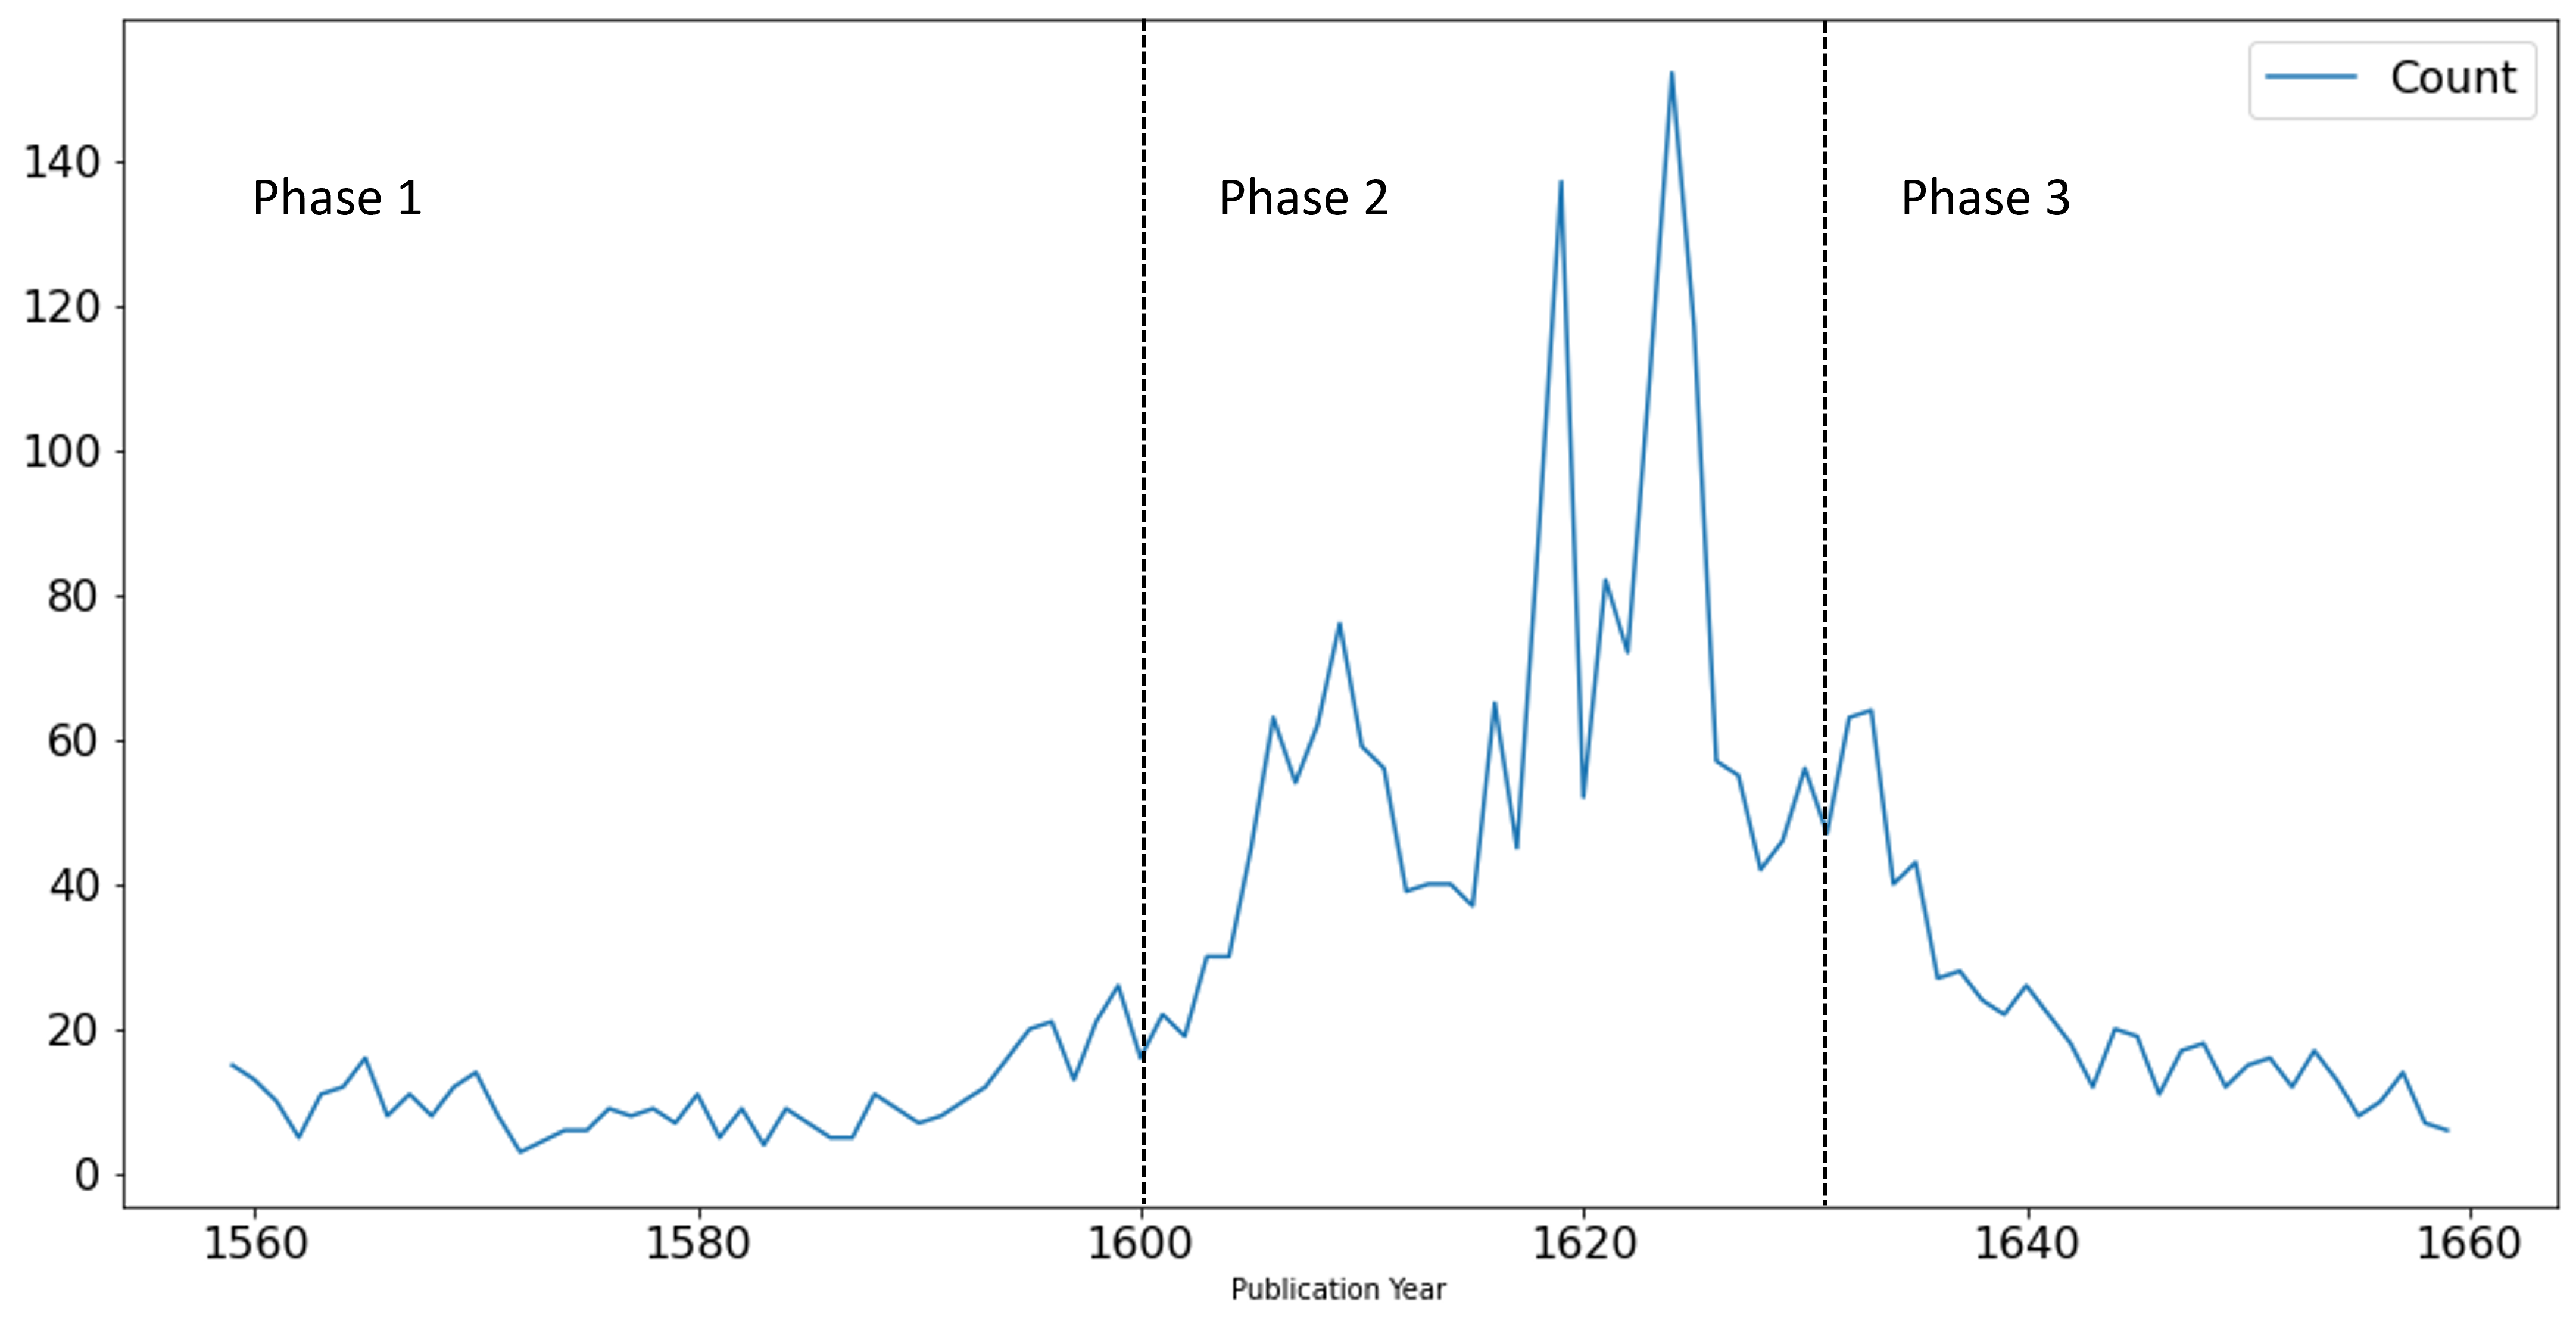
\includegraphics[scale=0.4]{graph/Overall Trend of the Douai Publishing Industry.png}
\caption{Overall Trend of the Douai Publishing Industry}
\label{fig:overallTrend}
\end{figure}

Moreover, if examining the trends of each language (Figure \ref{fig:lanTrend}), it becomes apparent that the trend of Latin publications closely aligns with the overall trend. Nevertheless, since Latin publications dominate this dataset, they occupy the most space in the line graph. As a result, it can be challenging to describe the details of the industry development from the graph, particularly regarding the involvement of individuals from the English region. This is where drawing the Network can compensate for this deficiency.

\begin{figure}[H]
\centering
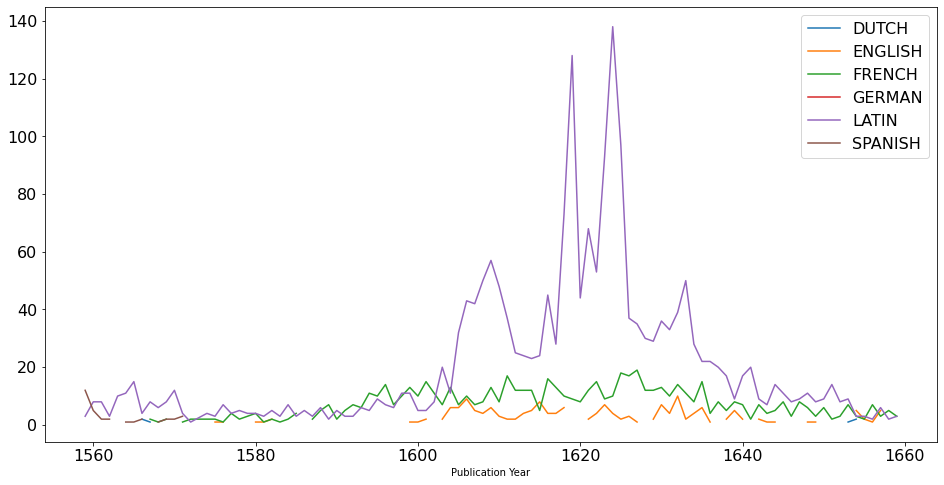
\includegraphics[scale=0.4]{graph/Trend of Languages.png}
\caption{Trend of Languages}
\label{fig:lanTrend}
\end{figure}

\pagebreak
Figure \ref{fig:peoNet} illustrates the overall Network of people in this dataset. The nodes of this Network are every person in the dataset and their size represents their Degree. In other words, the more people a person is connected to, the bigger the size of the node this person will have. Each edge is a publication. It connects two people (nodes) who were involved in it and is coloured by its language.

\begin{figure}[H]
\centering
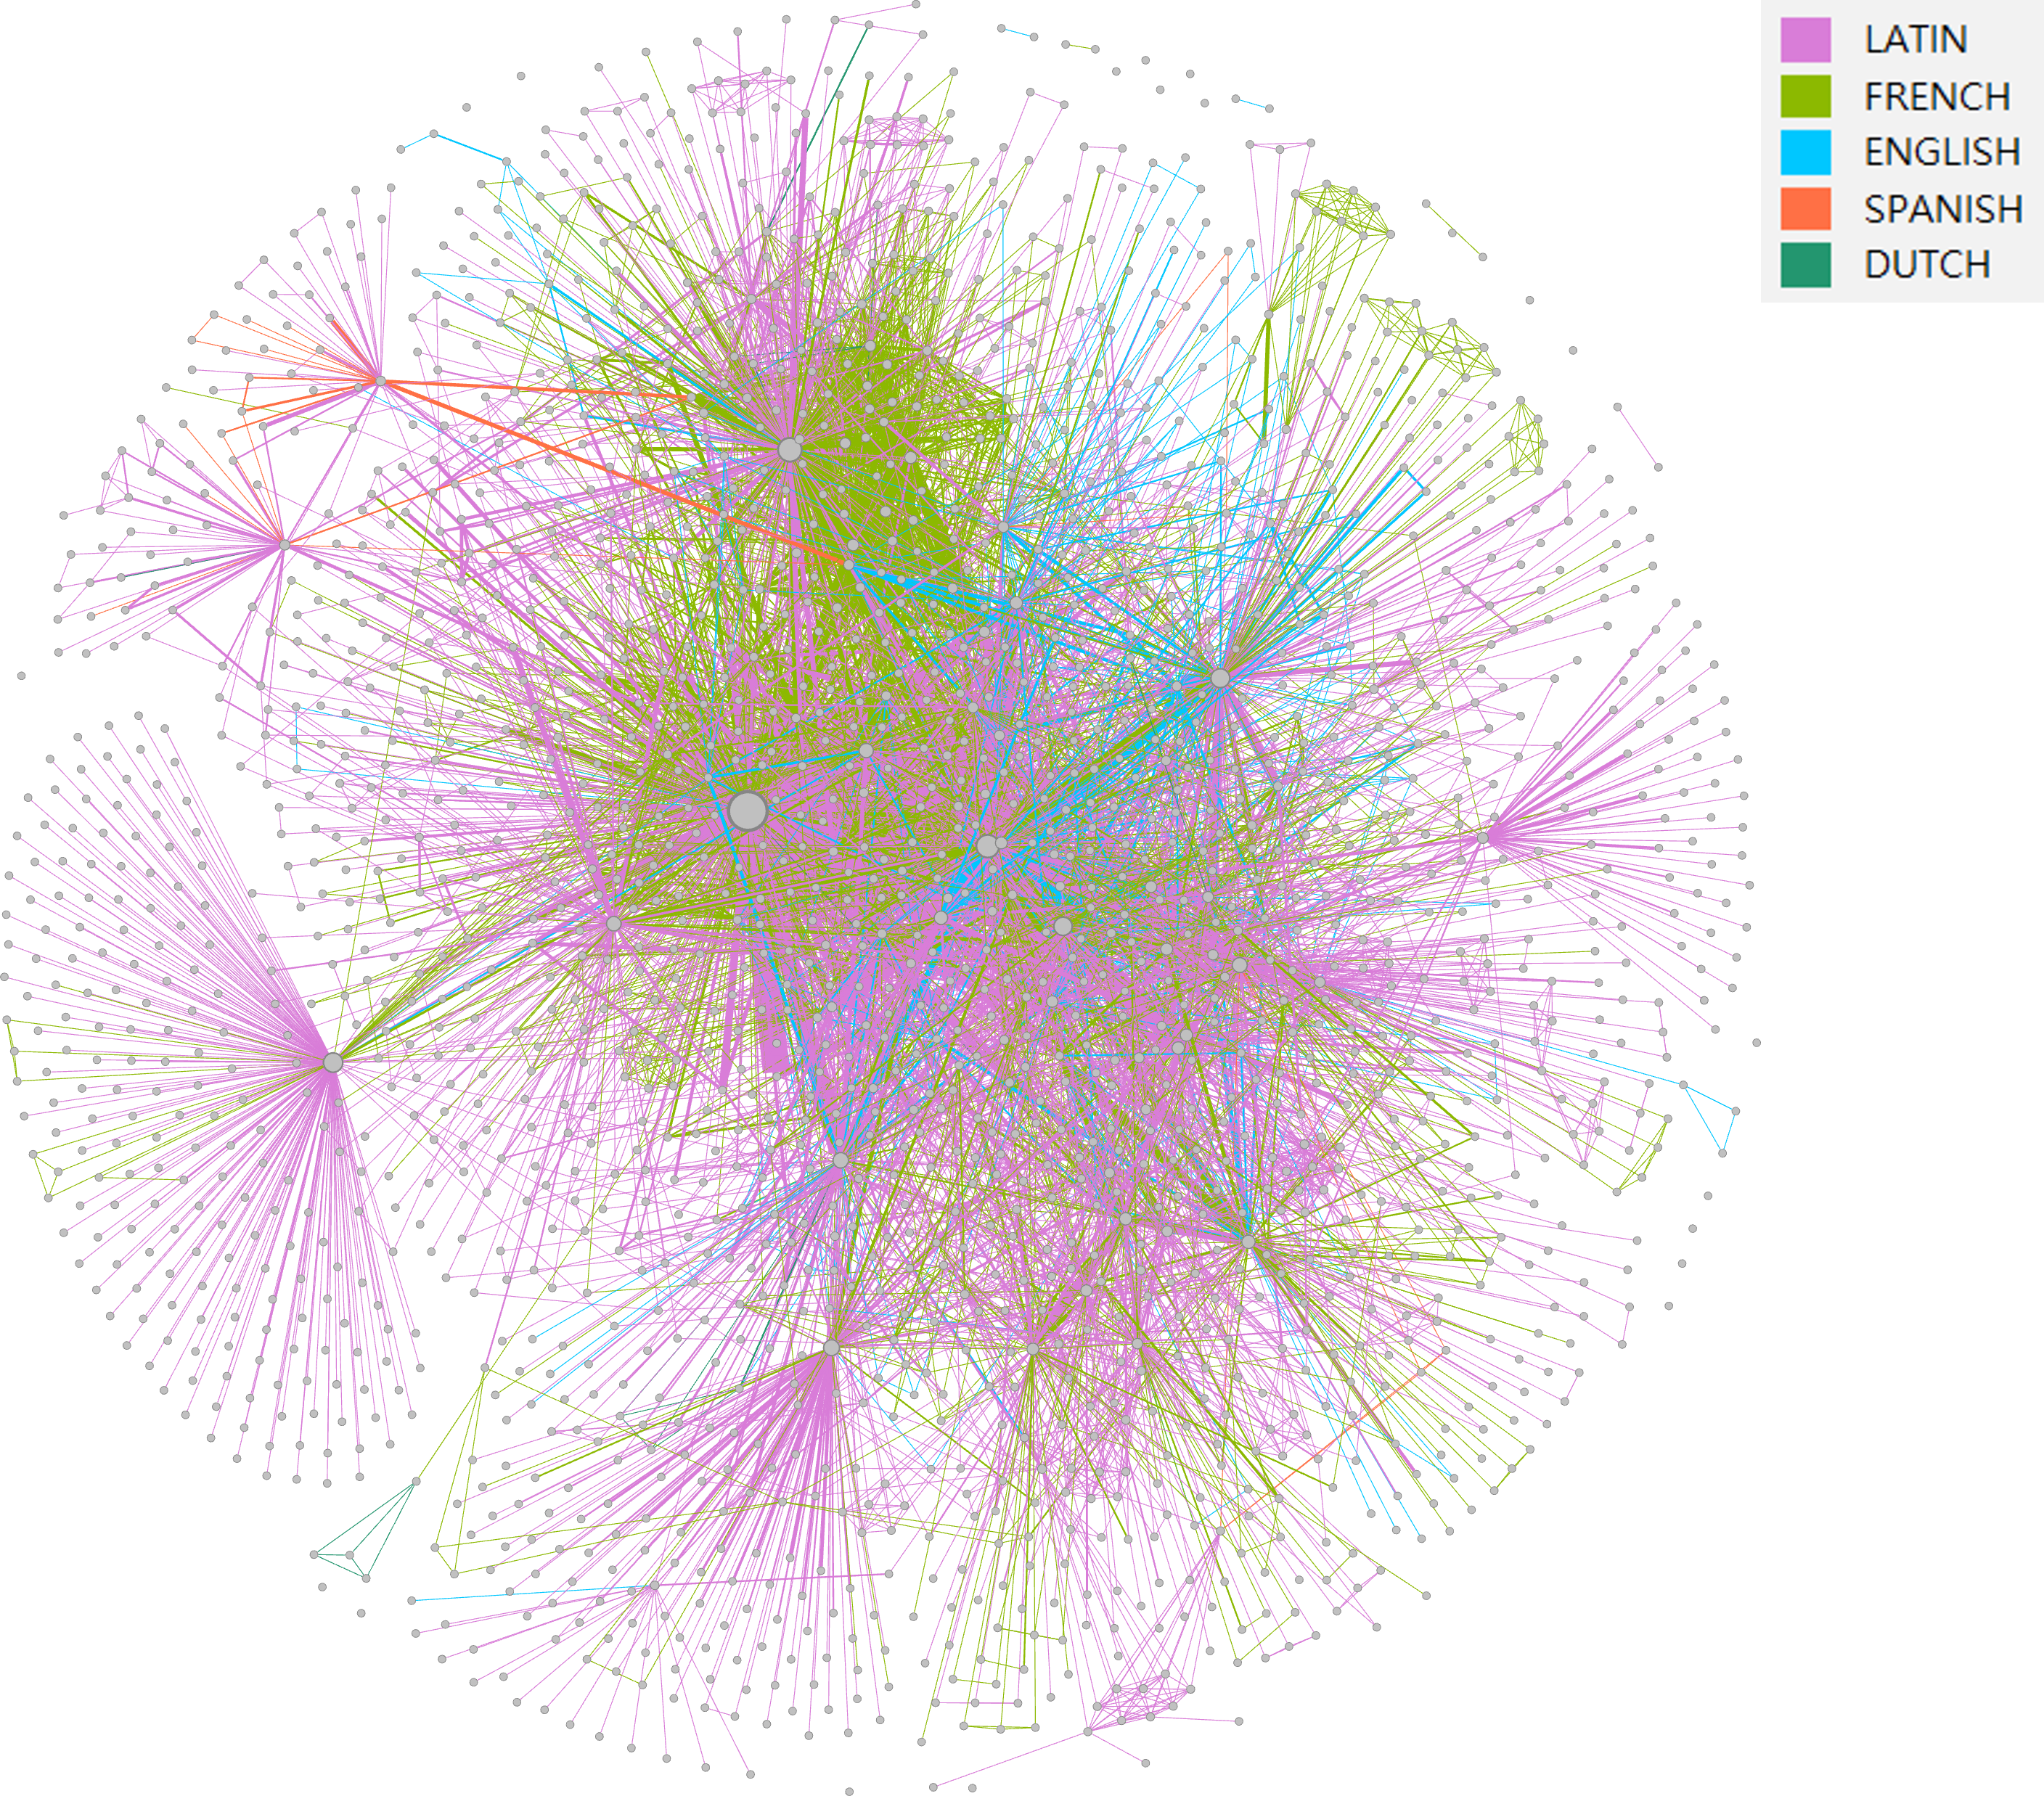
\includegraphics[scale=0.6]{graph/The People Network.png}
\caption{The People Network}
\label{fig:peoNet}
\end{figure}

Figure \ref{fig:peoNetBefore1600} shows the trend of the People Network before the 1600s. Interestingly, Spanish publications emerged in the Network before any other languages, implying that there were already some printers/publishers operating in Douai before the development of its publishing industry. Since Douai belonged to the Spanish (Habsburg) Netherlands at that time (De Ridder et al., 2020; Soen, 2015; Soen et al., 2019; Soen \& Junot, 2021), the audience of these printers/publishers could have been from the Habsburg Spain.

Later, French publications took up the largest portion of the Network before the 1600s. Since French was the main local language around Douai during this era (Soen et al., 2015; Soetaert, 2019a, 2014; Soetaert \& Soen, 2020a), there were lots of Spanish or Italian religious publications translated into French by local clergy (Soetaert, 2014). This may have led to the dominance of French publications in the Network. Therefore, we can assume that, during the beginning phase of the Douai publishing industry, its main target audience consisted of people using French within the local area.

\begin{figure}[H]
\centering
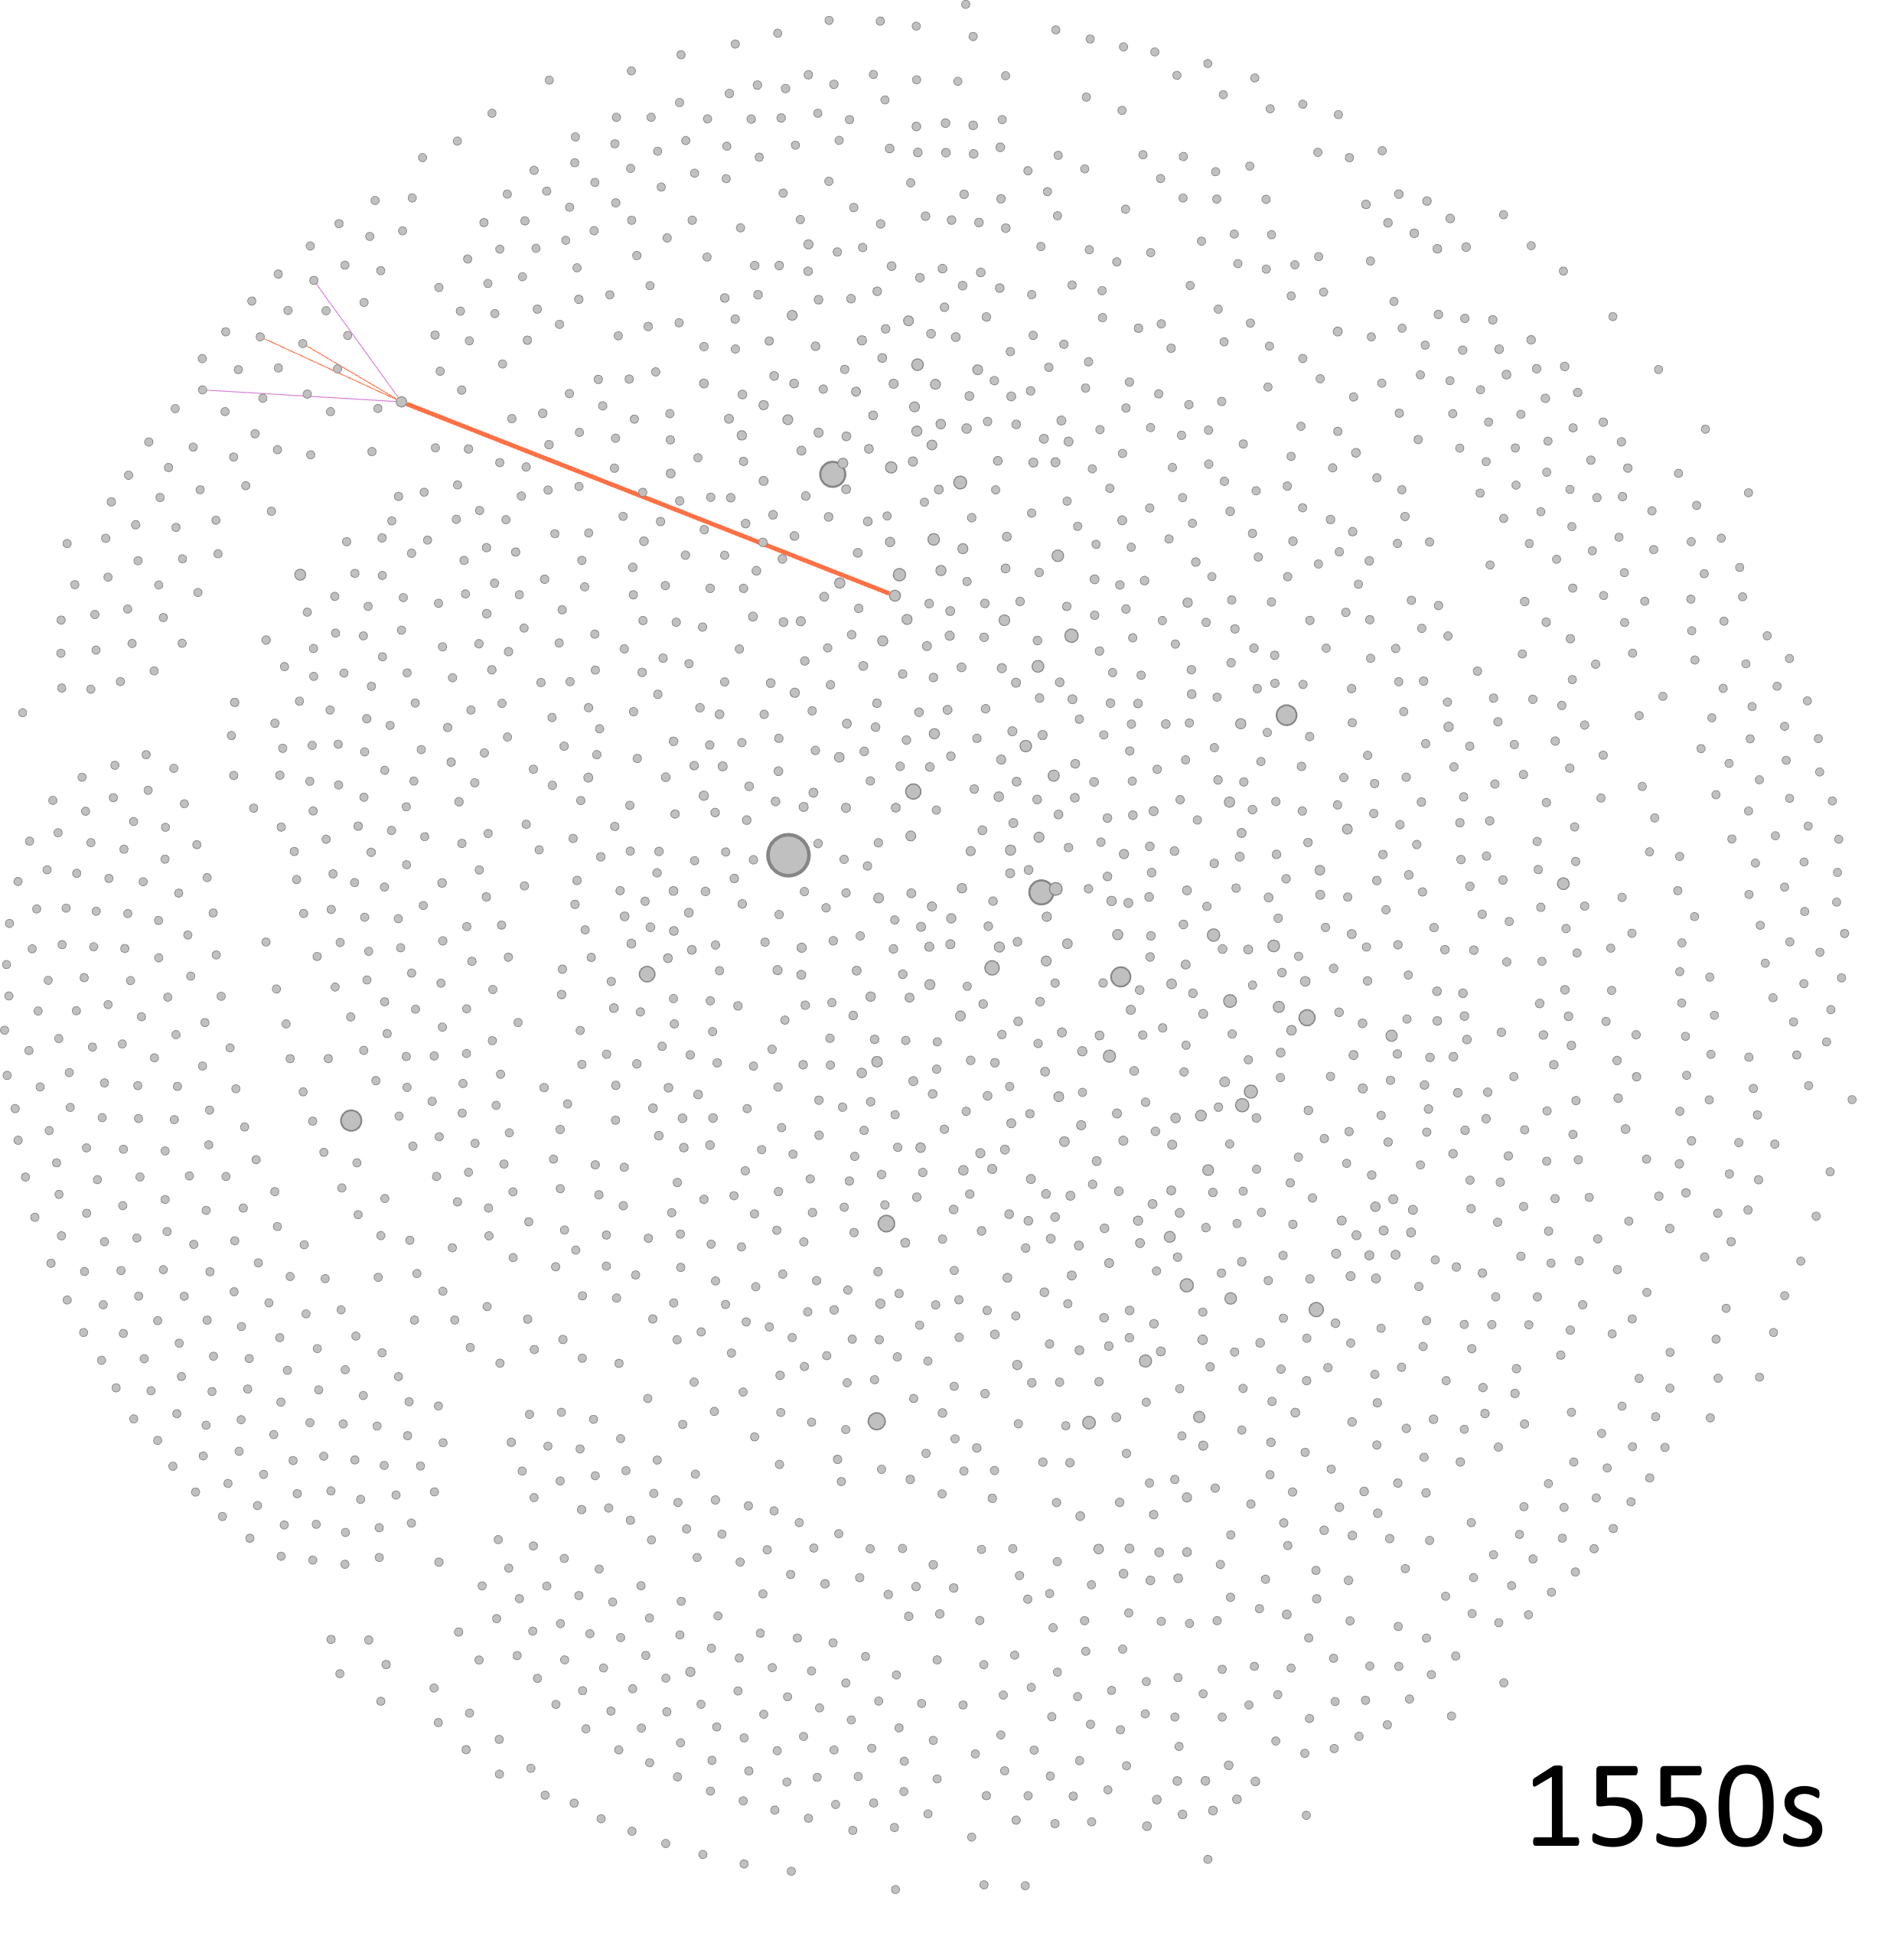
\includegraphics[scale=0.4]{graph/People_1550s.png}
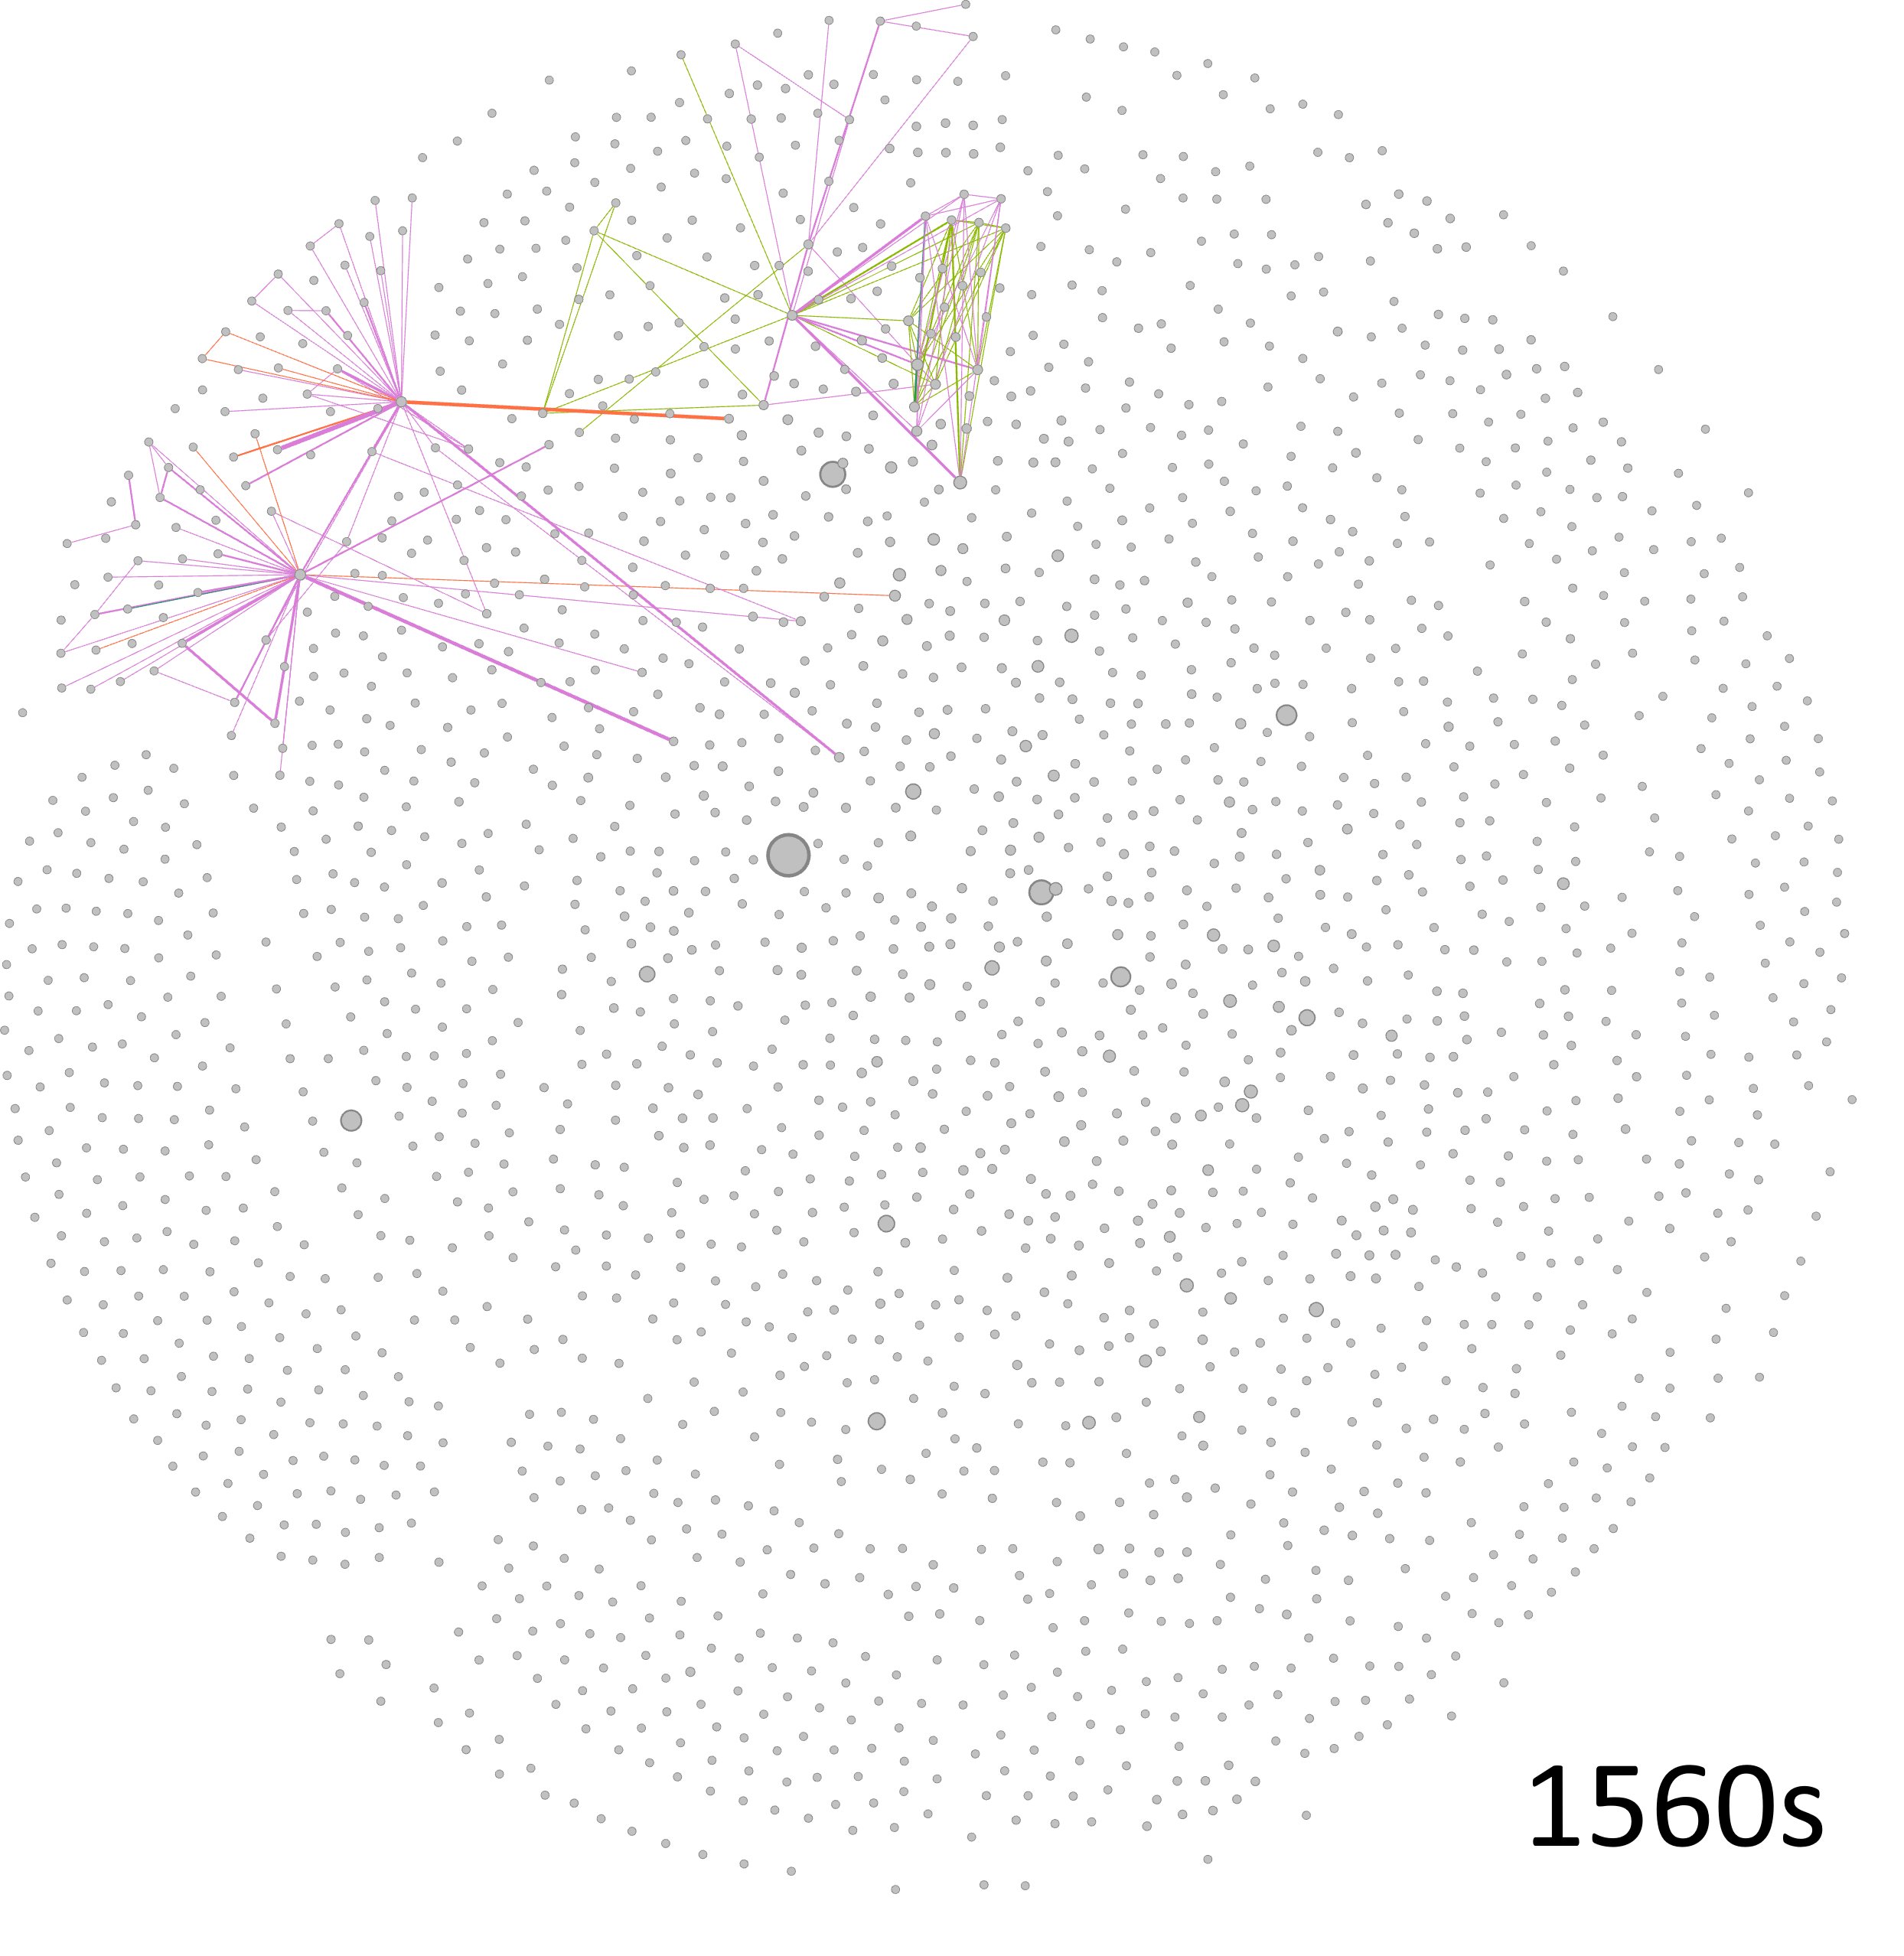
\includegraphics[scale=0.4]{graph/People_1560s.png}
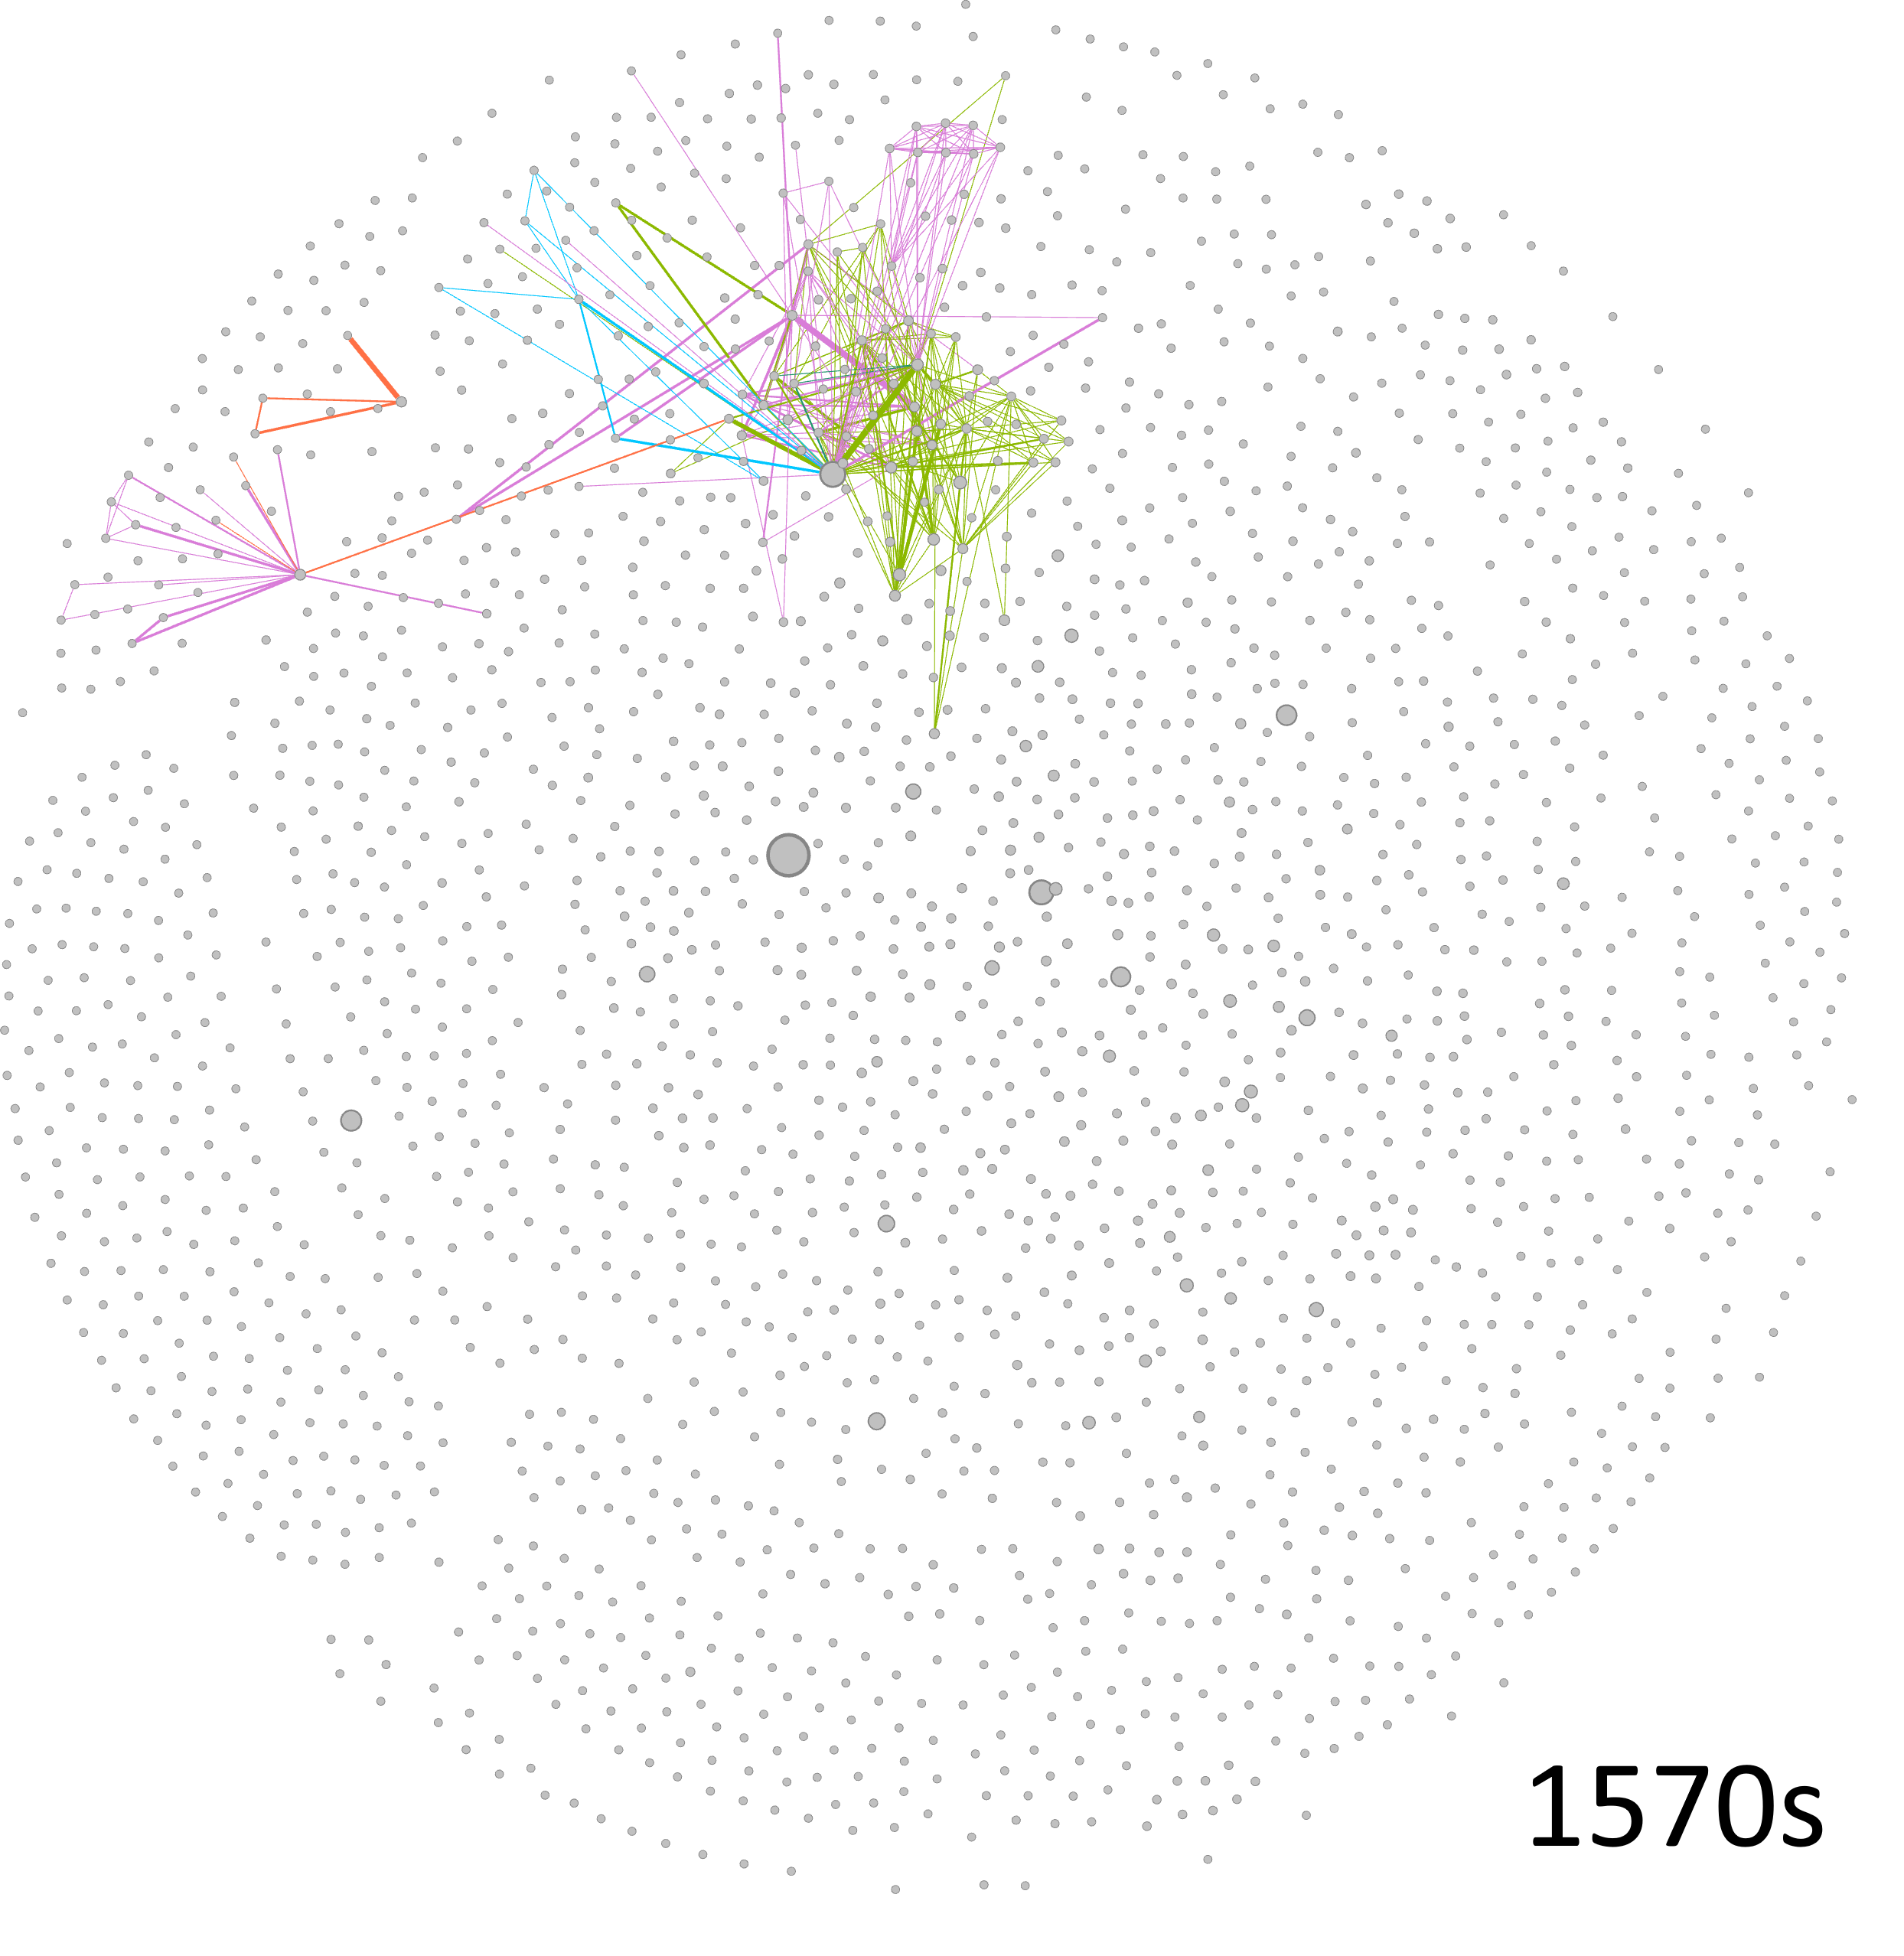
\includegraphics[scale=0.4]{graph/People_1570s.png}
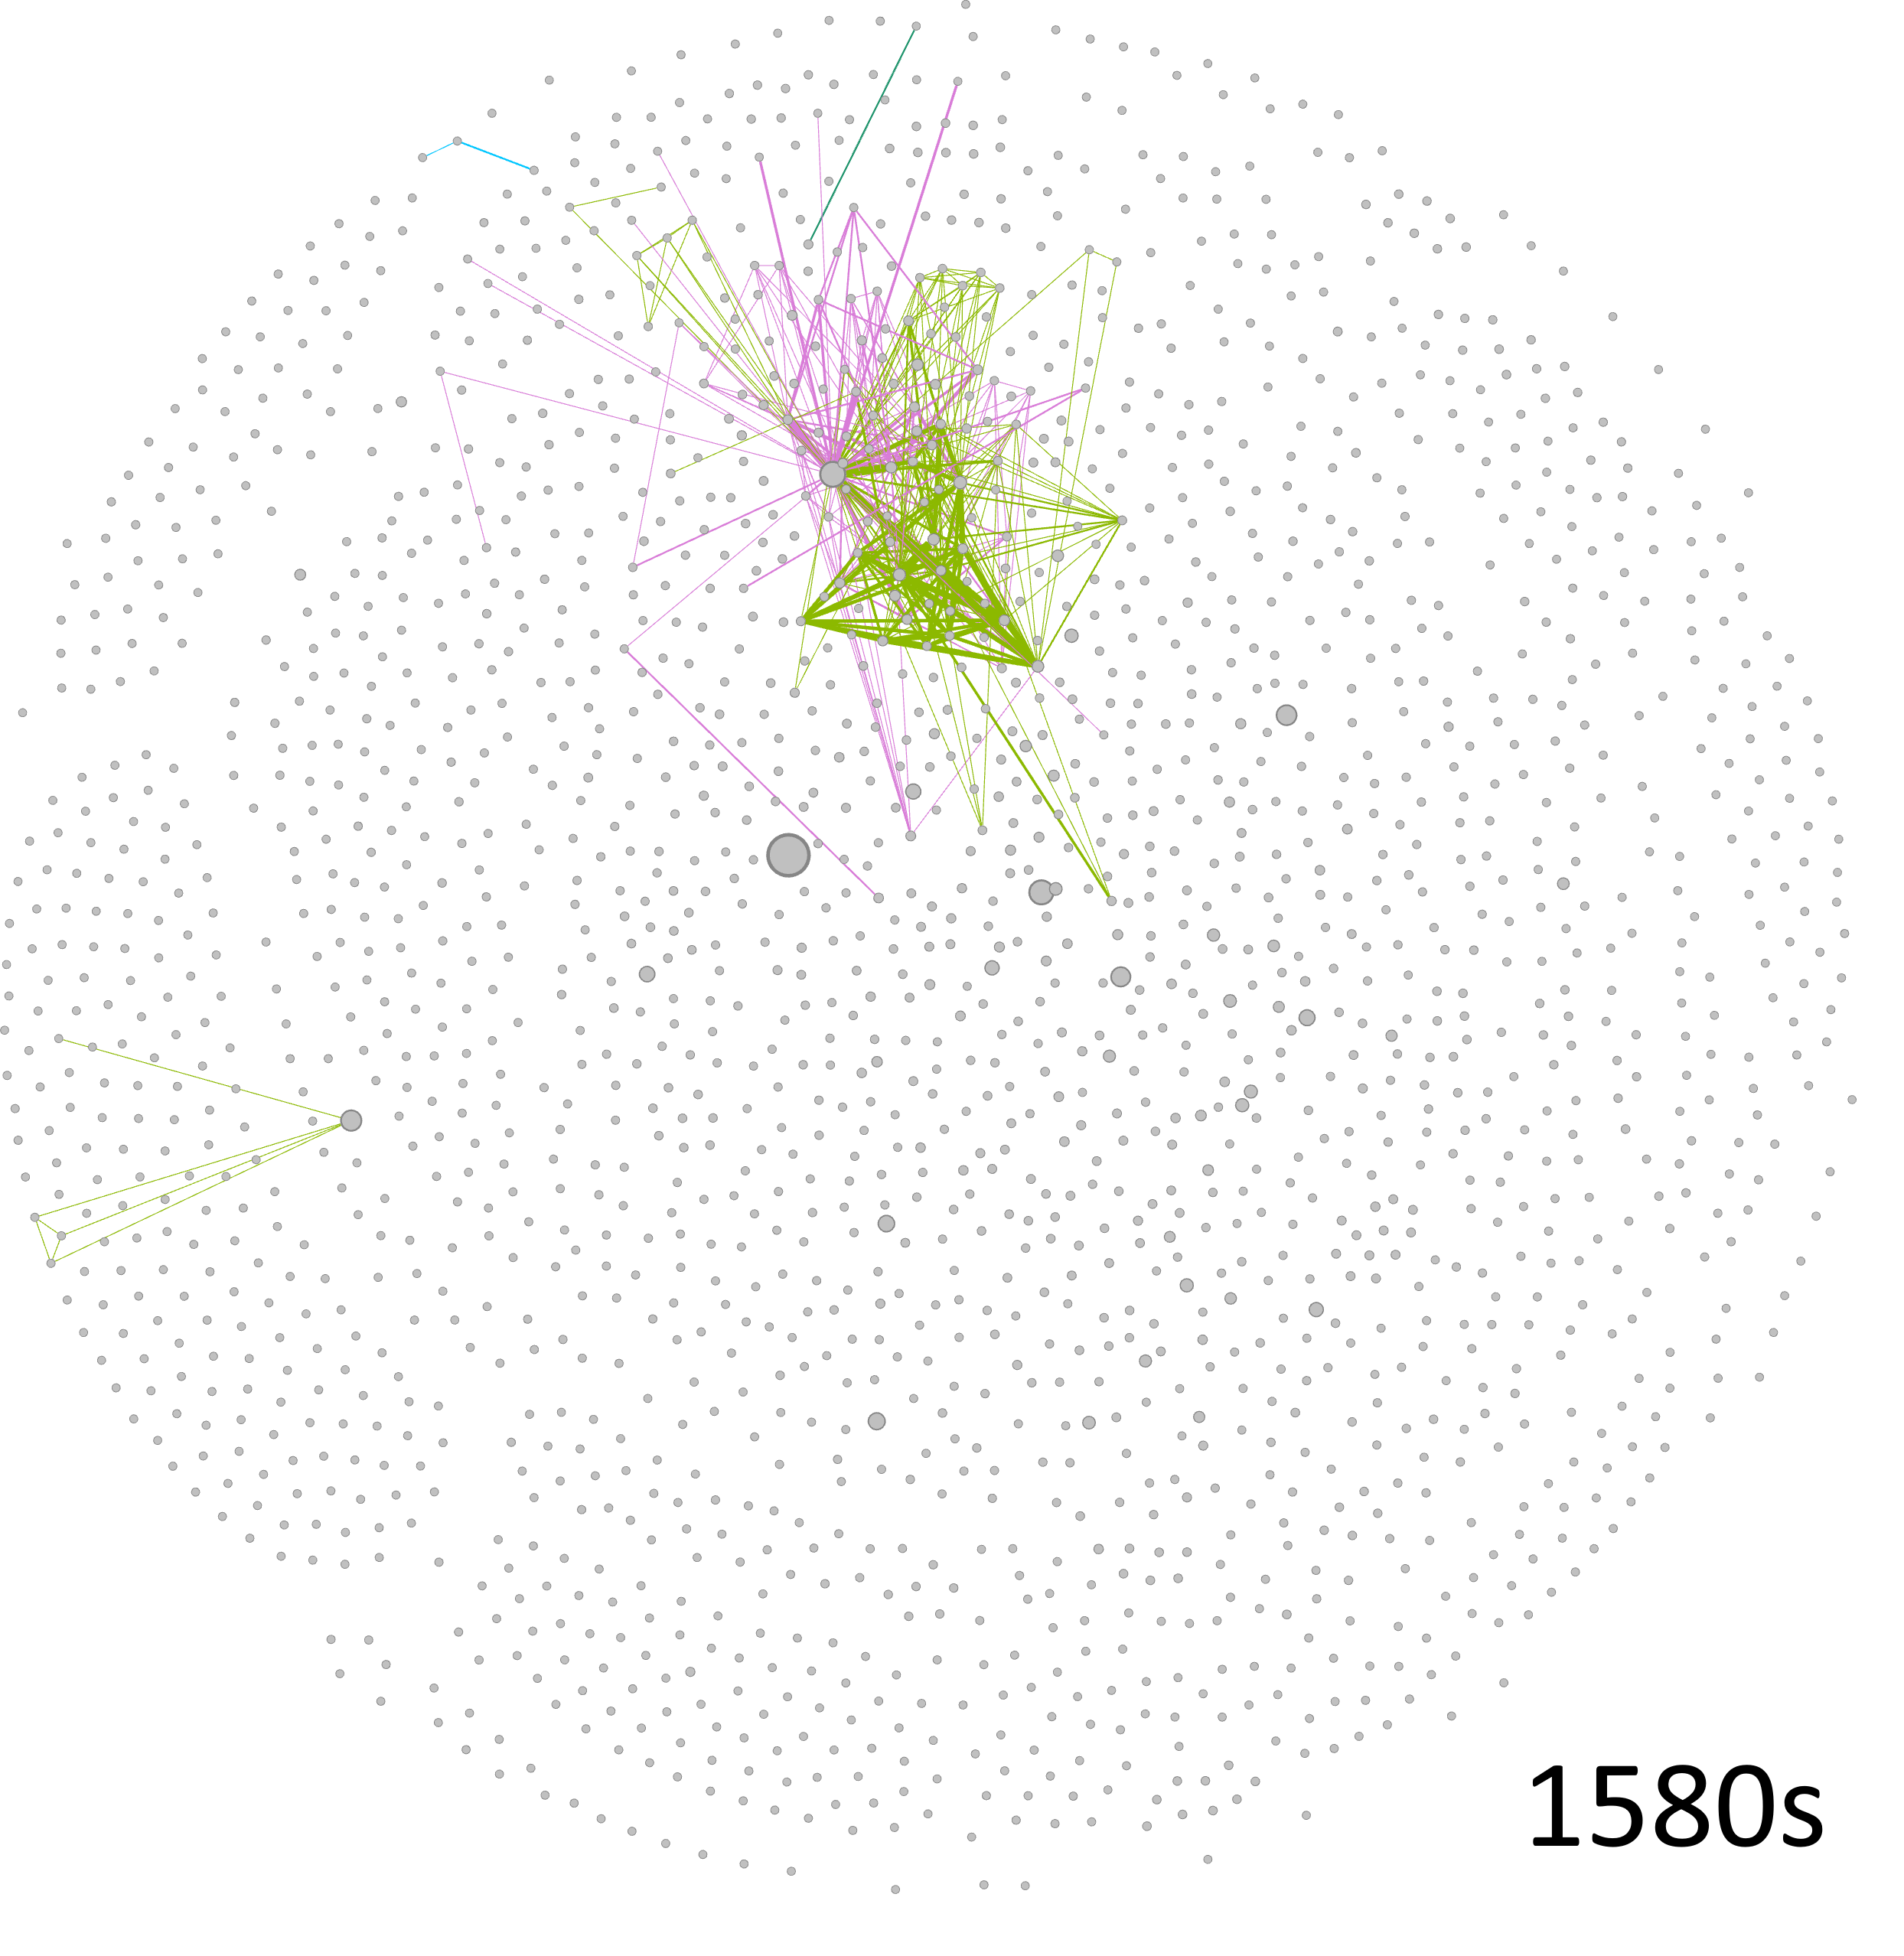
\includegraphics[scale=0.4]{graph/People_1580s.png}
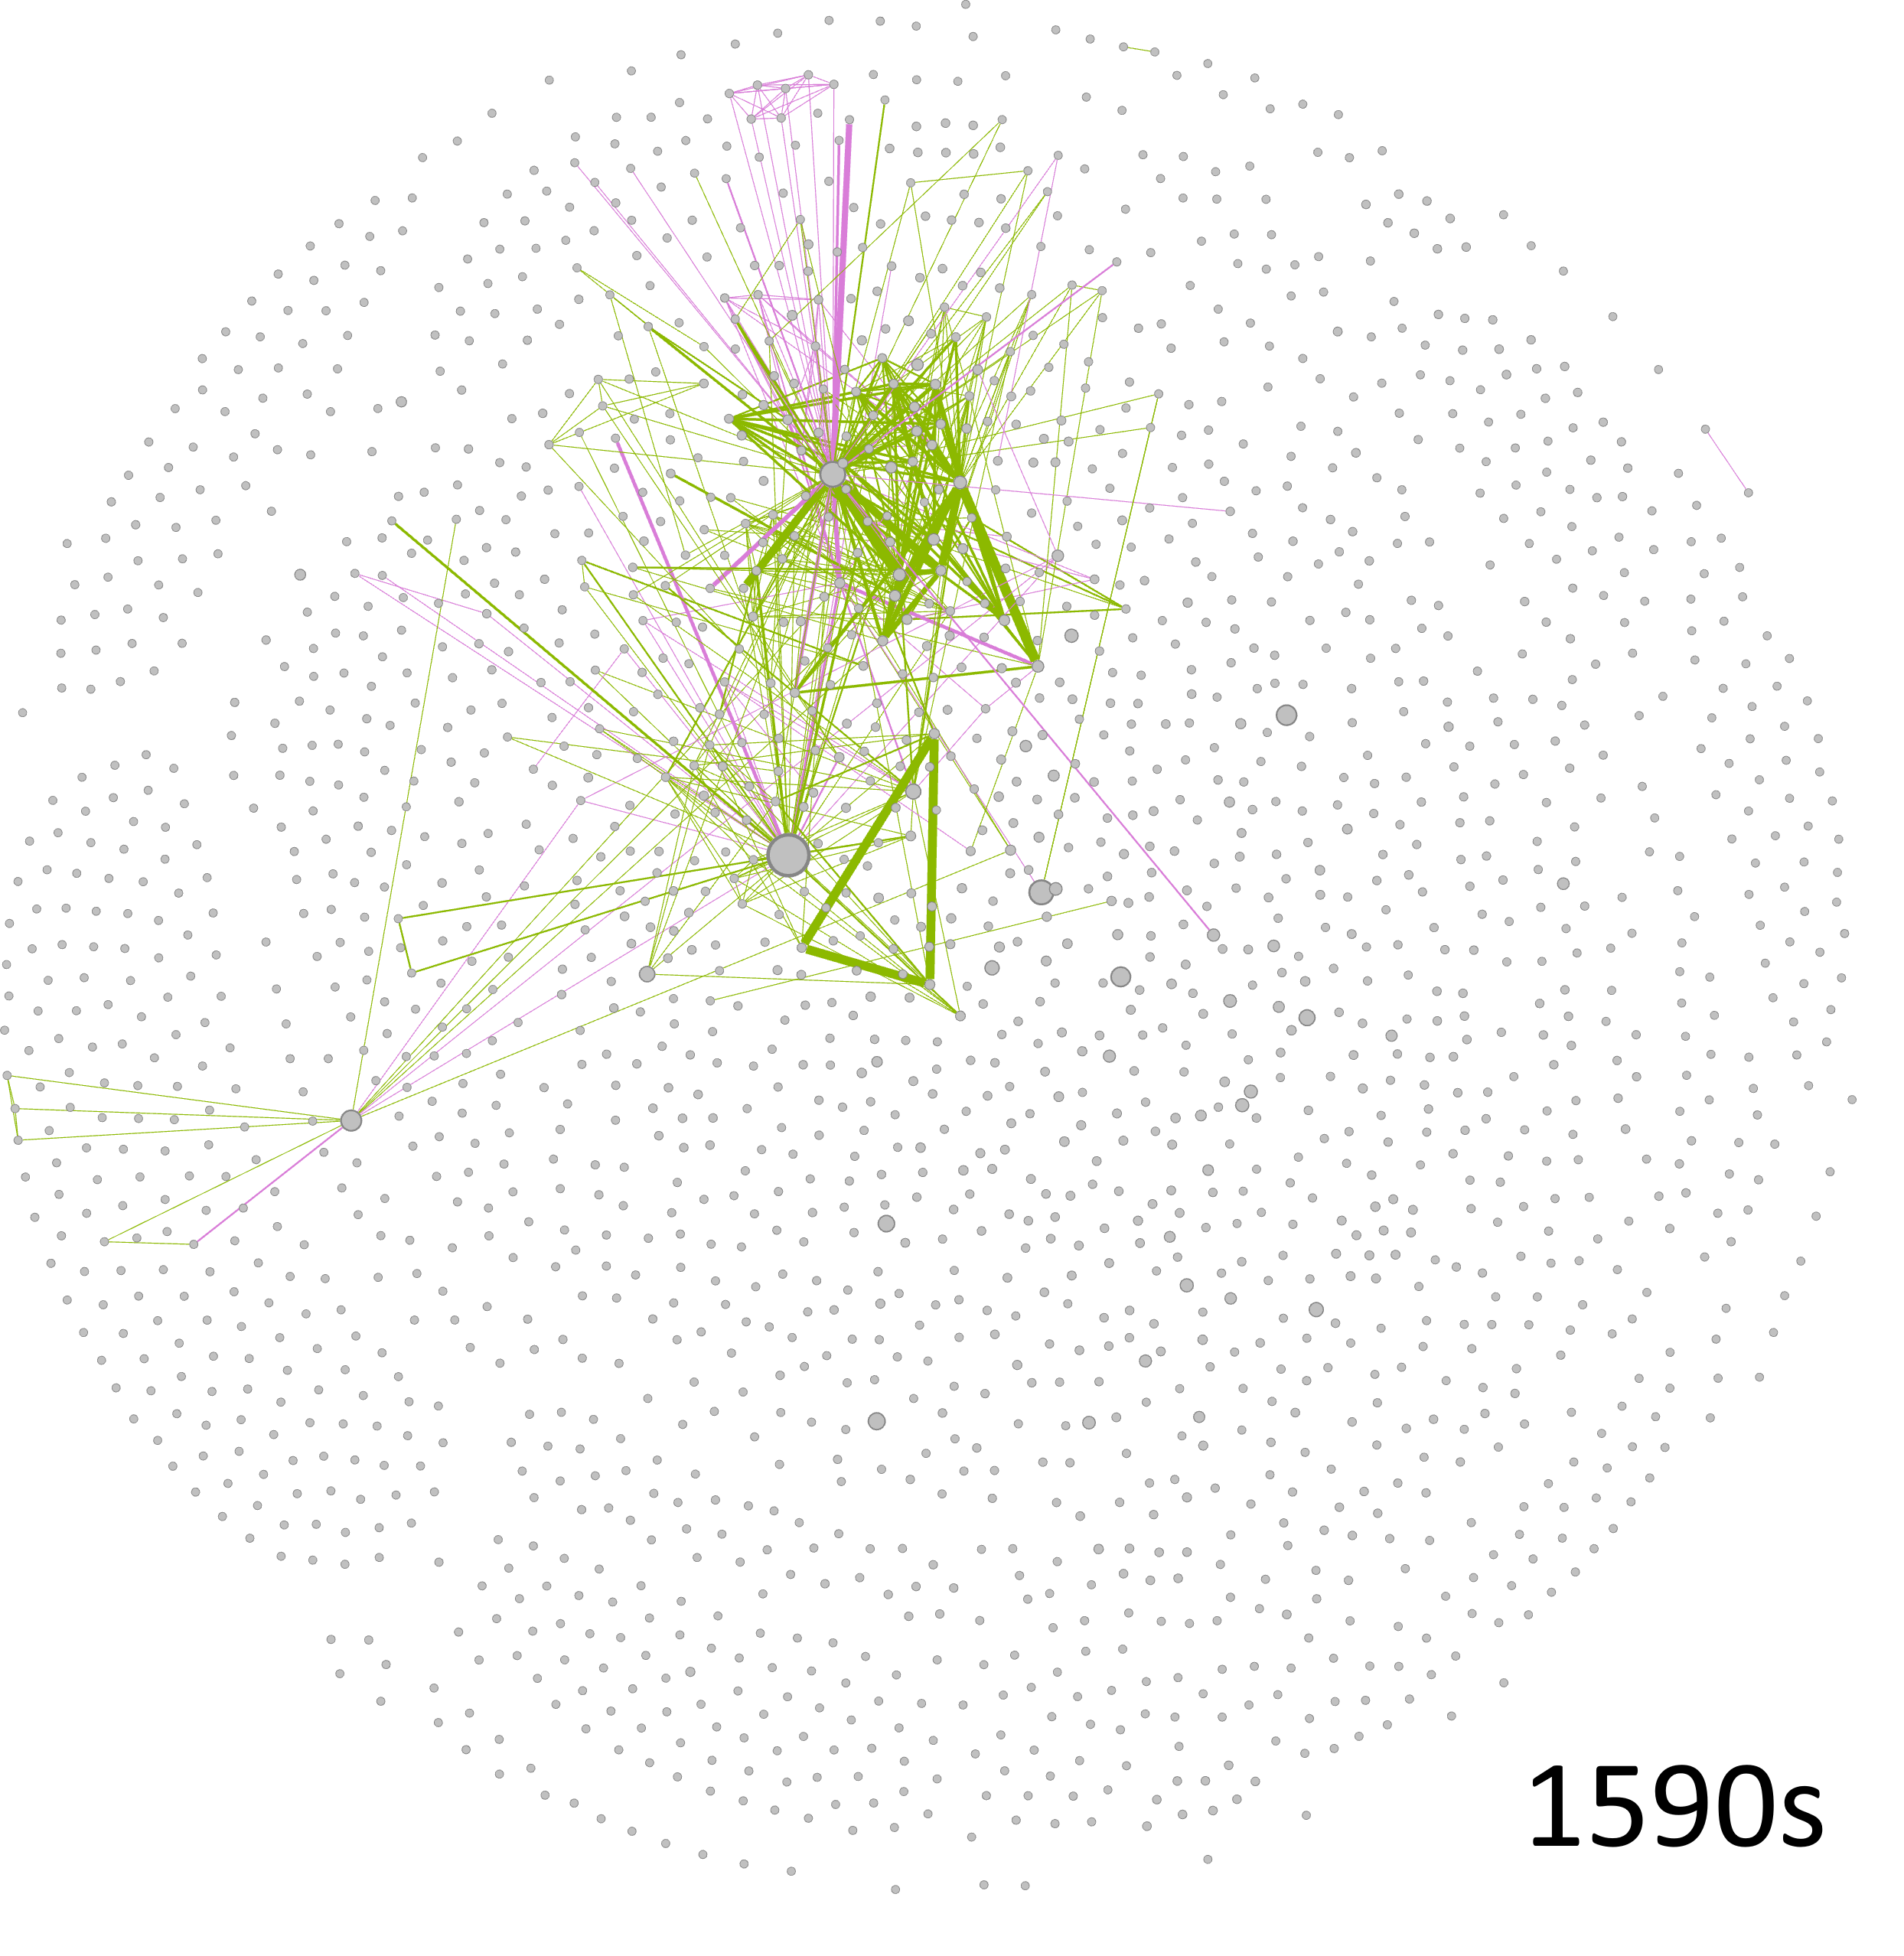
\includegraphics[scale=0.4]{graph/People_1590s.png}
% 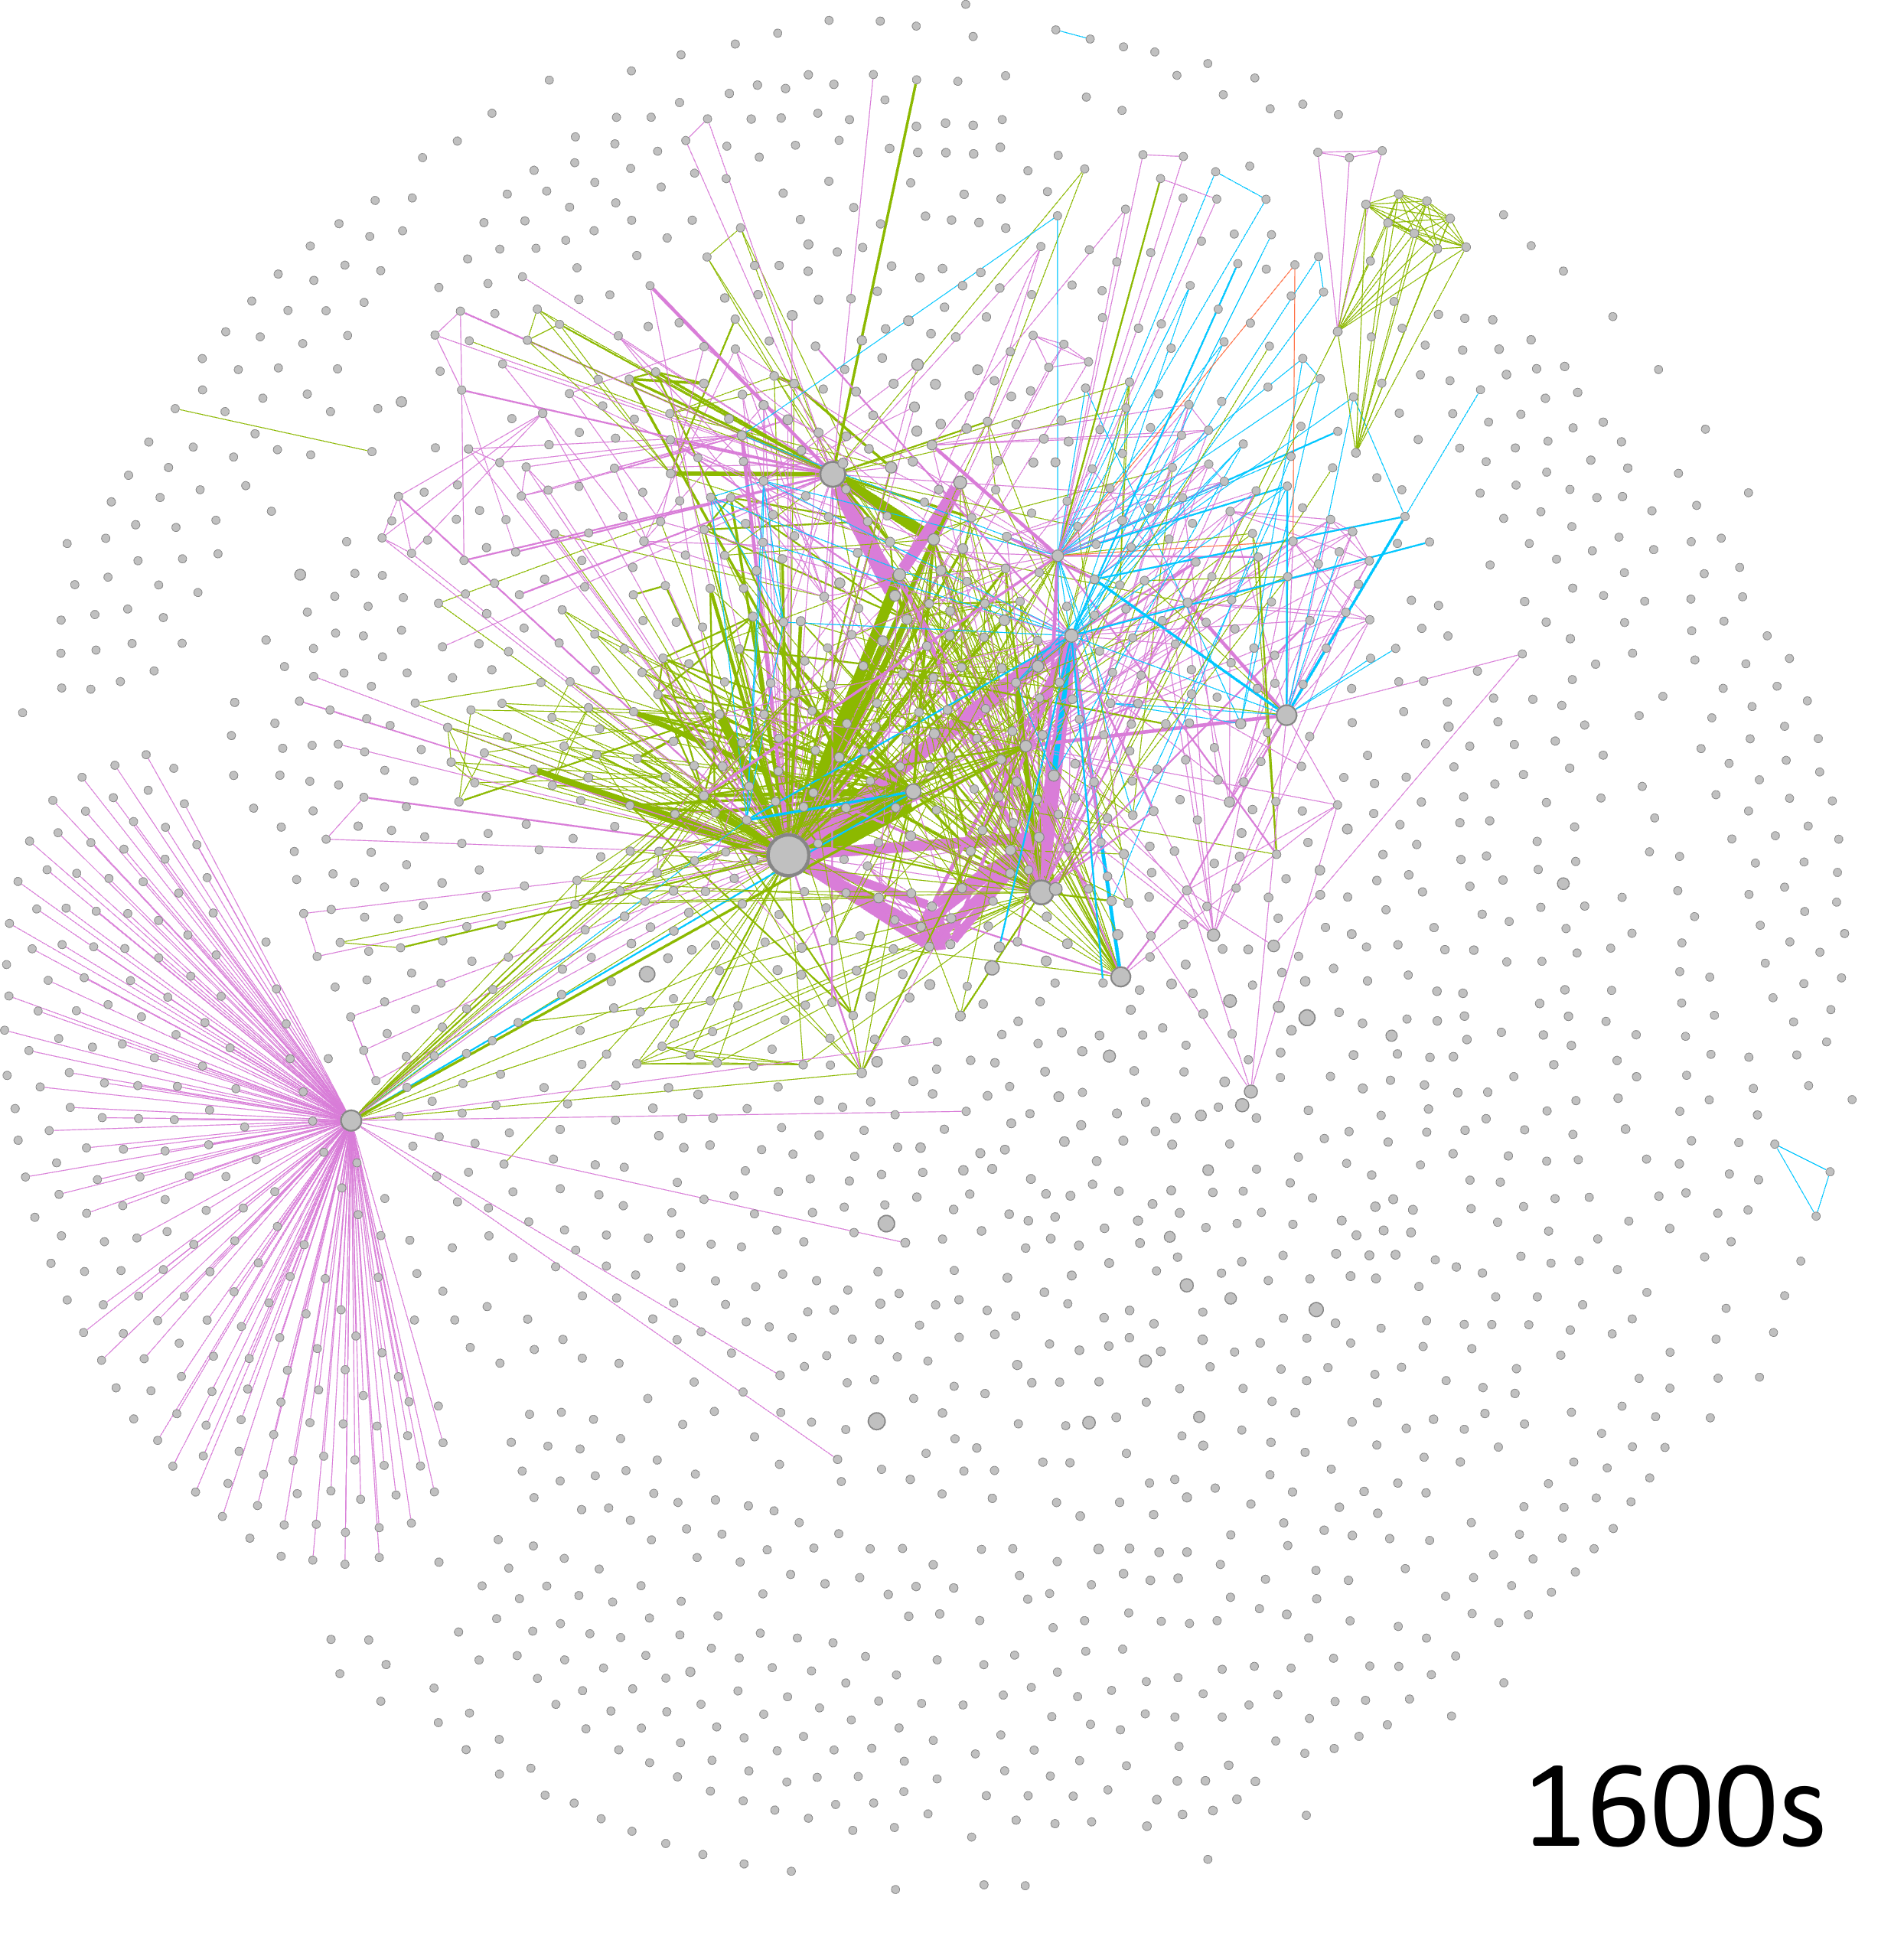
\includegraphics[scale=0.4]{graph/People_1600s.png}
\caption{Trend of the People Network before the 1600s}
\label{fig:peoNetBefore1600}
\end{figure}

\begin{figure}[H]
\centering
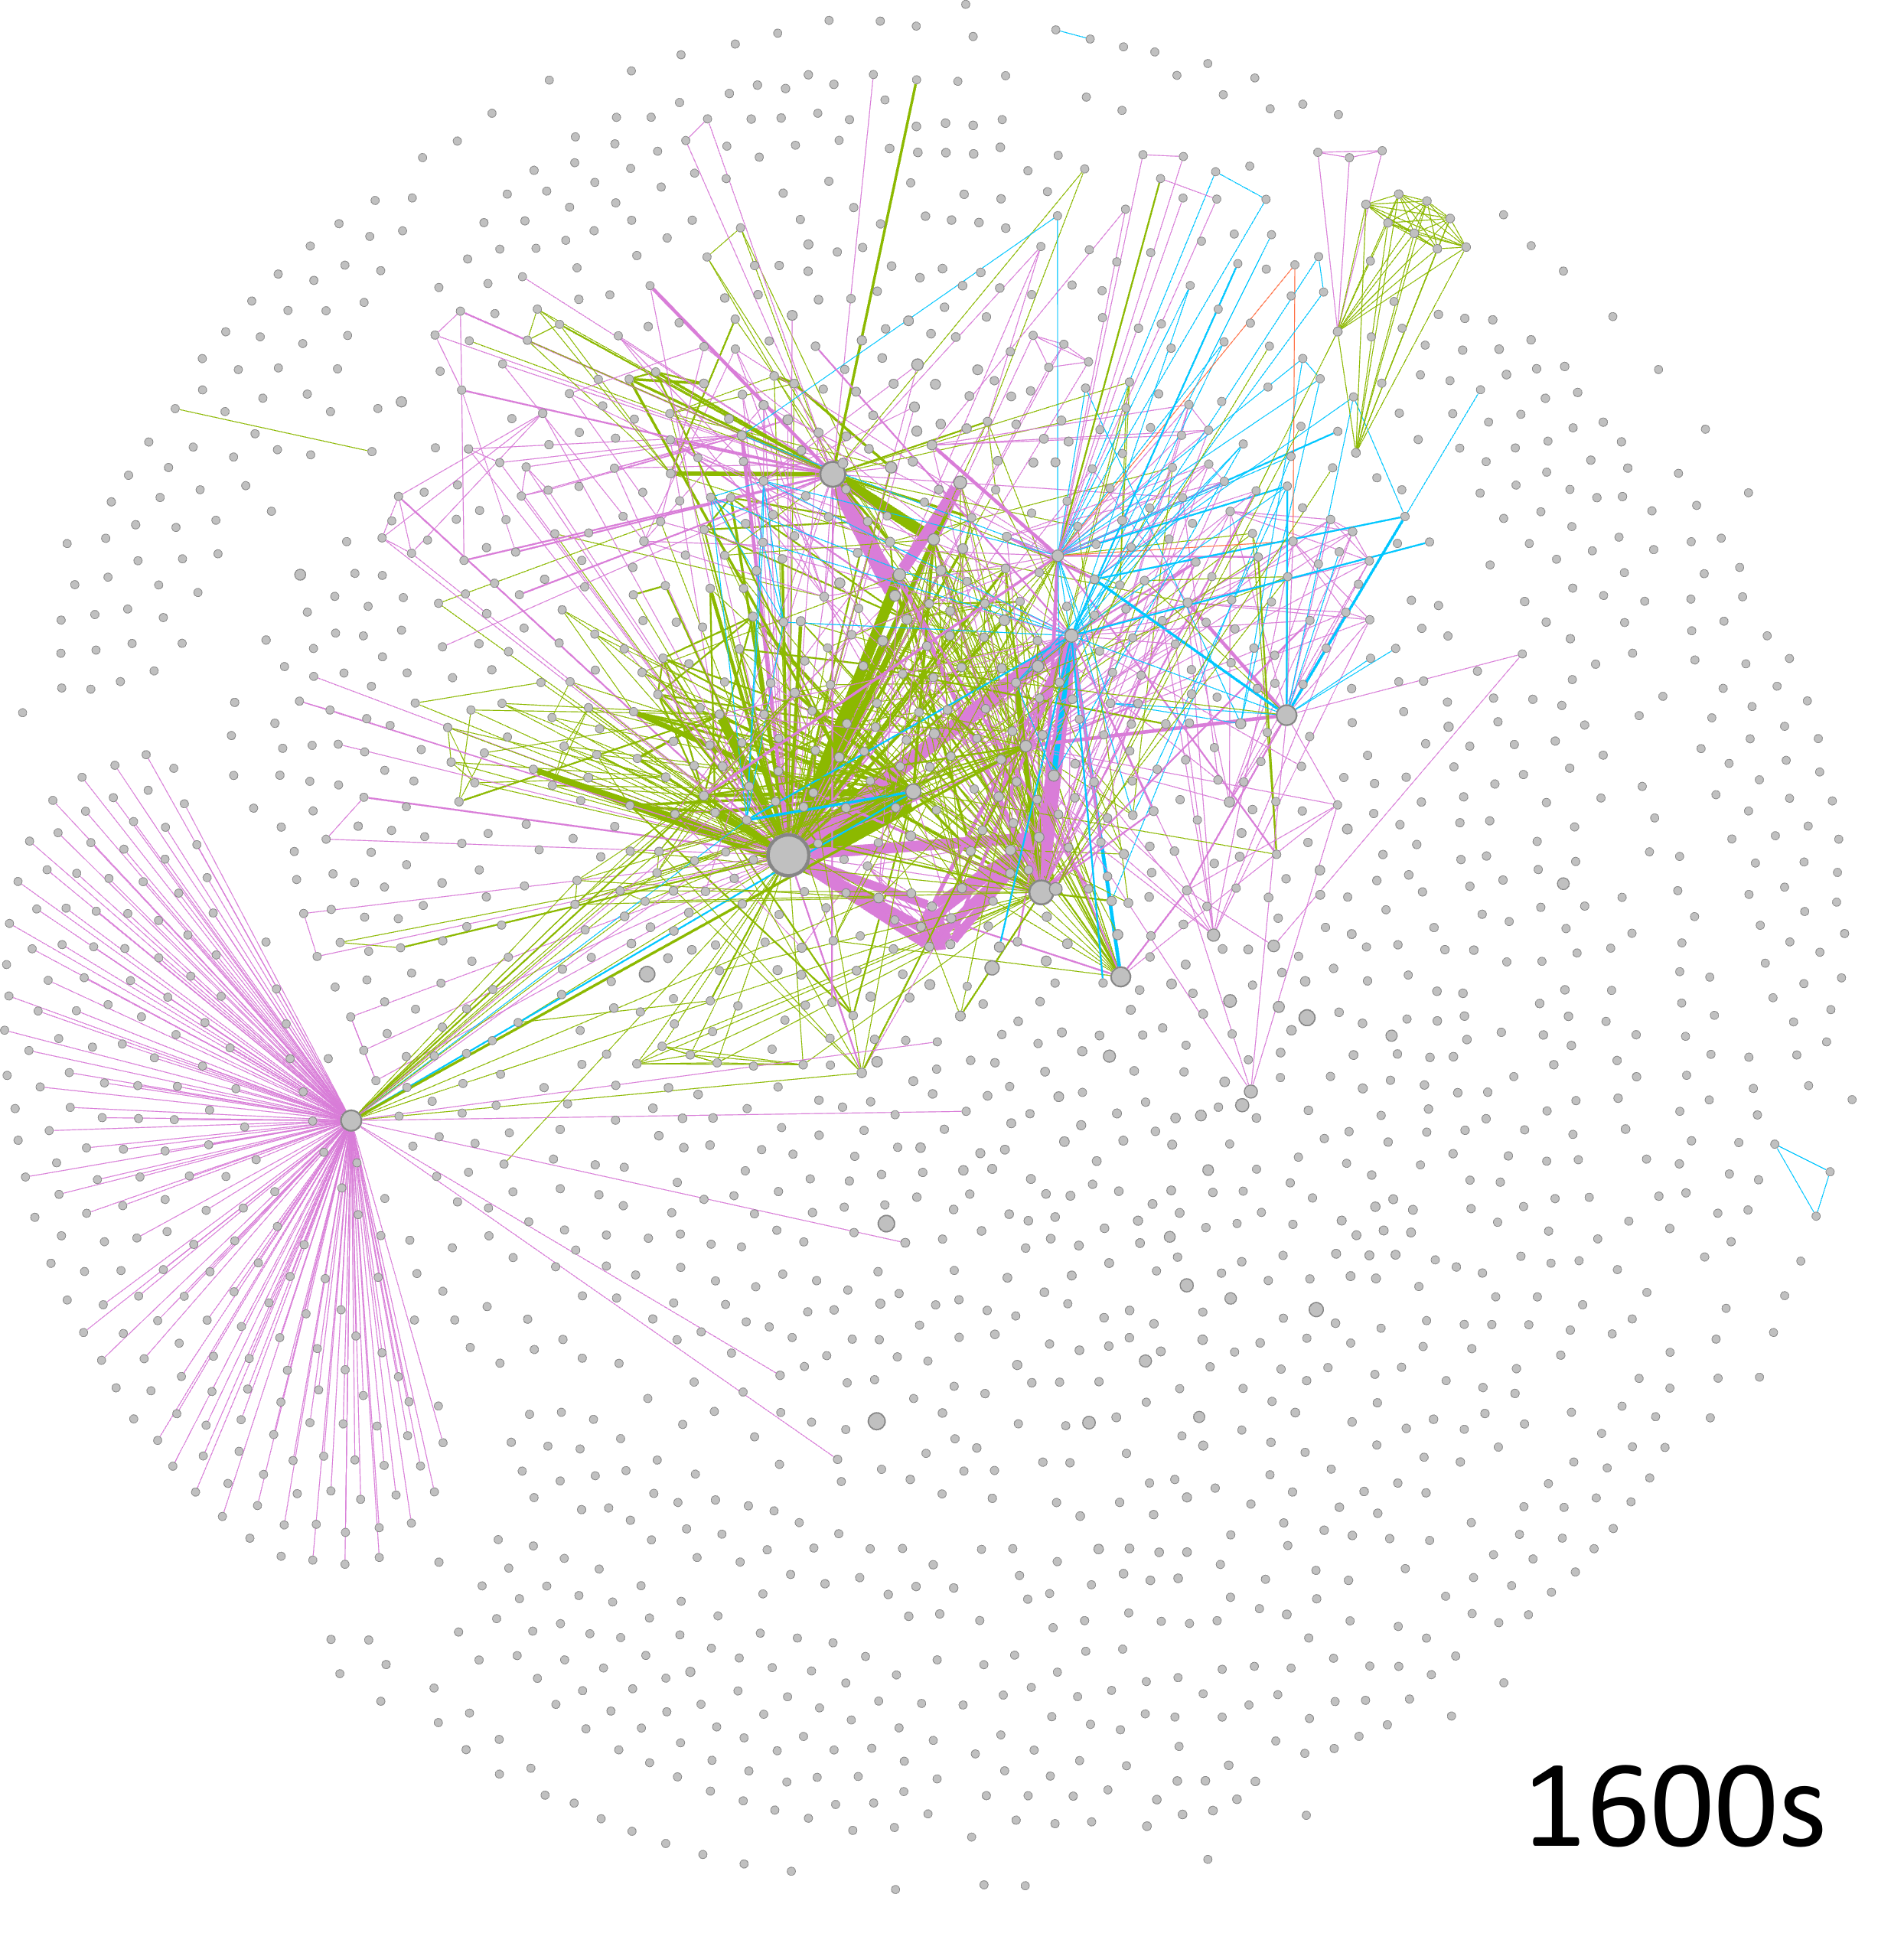
\includegraphics[scale=0.4]{graph/People_1600s.png}
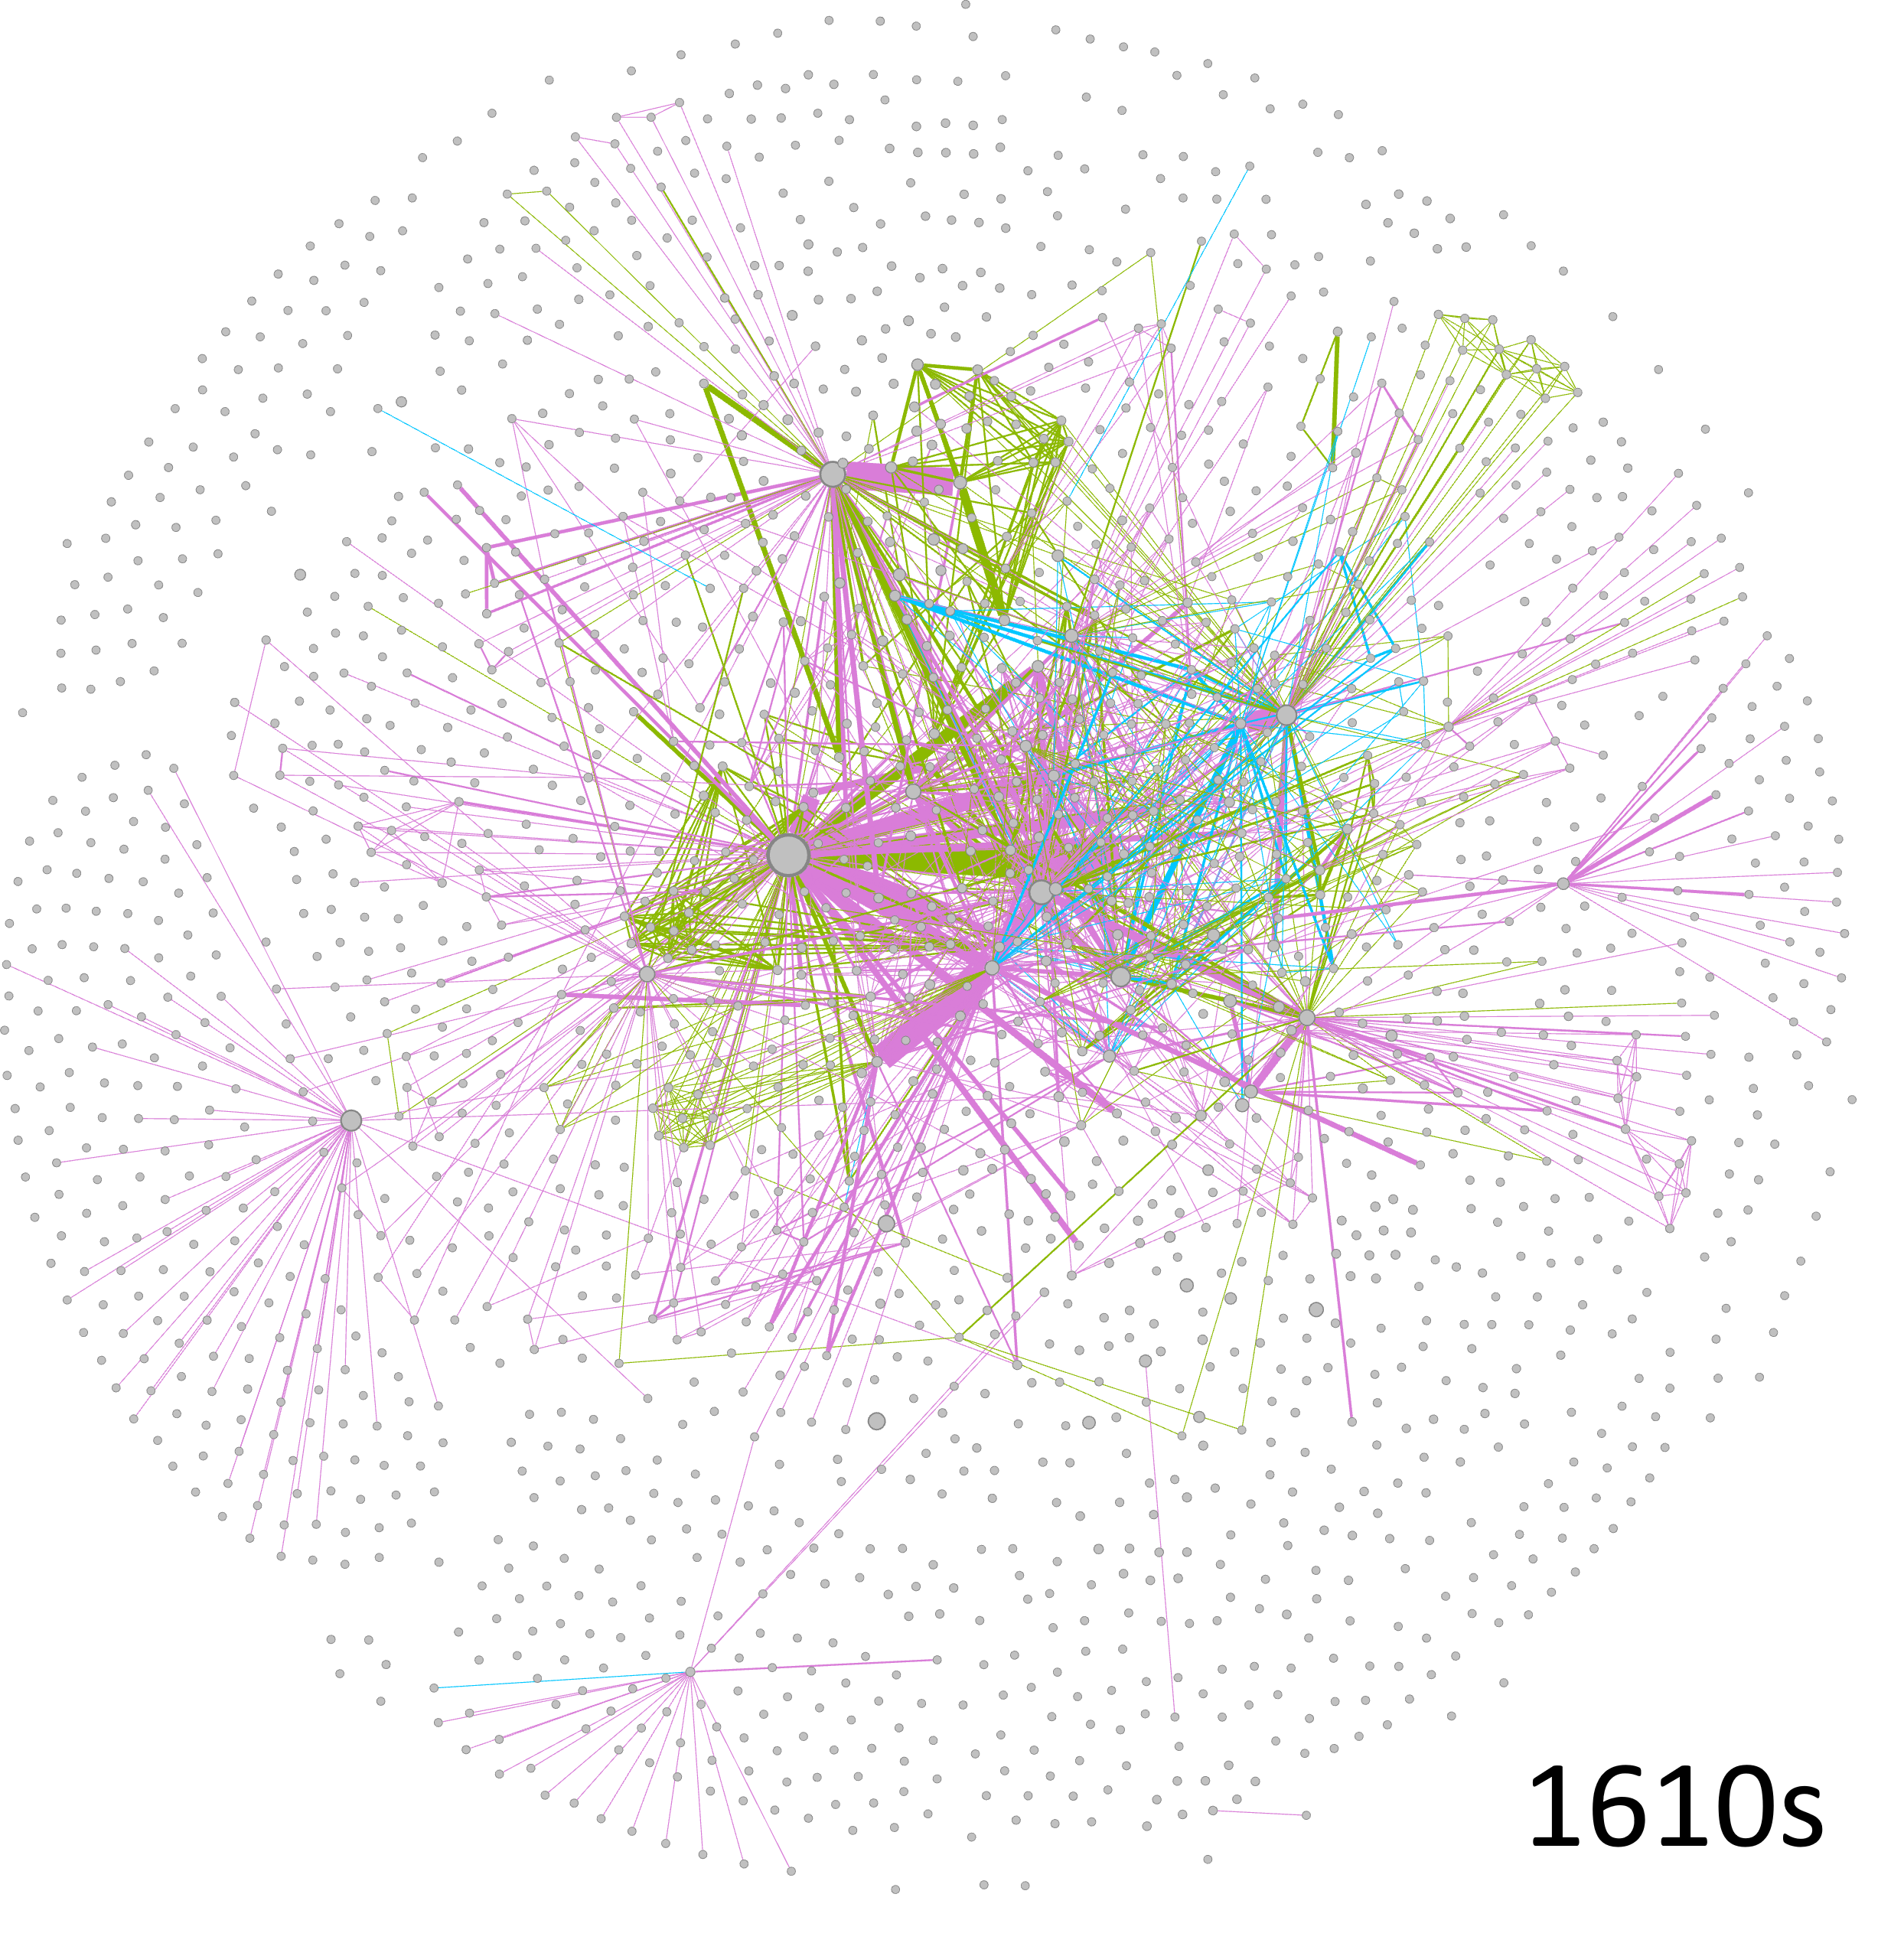
\includegraphics[scale=0.4]{graph/People_1610s.png}
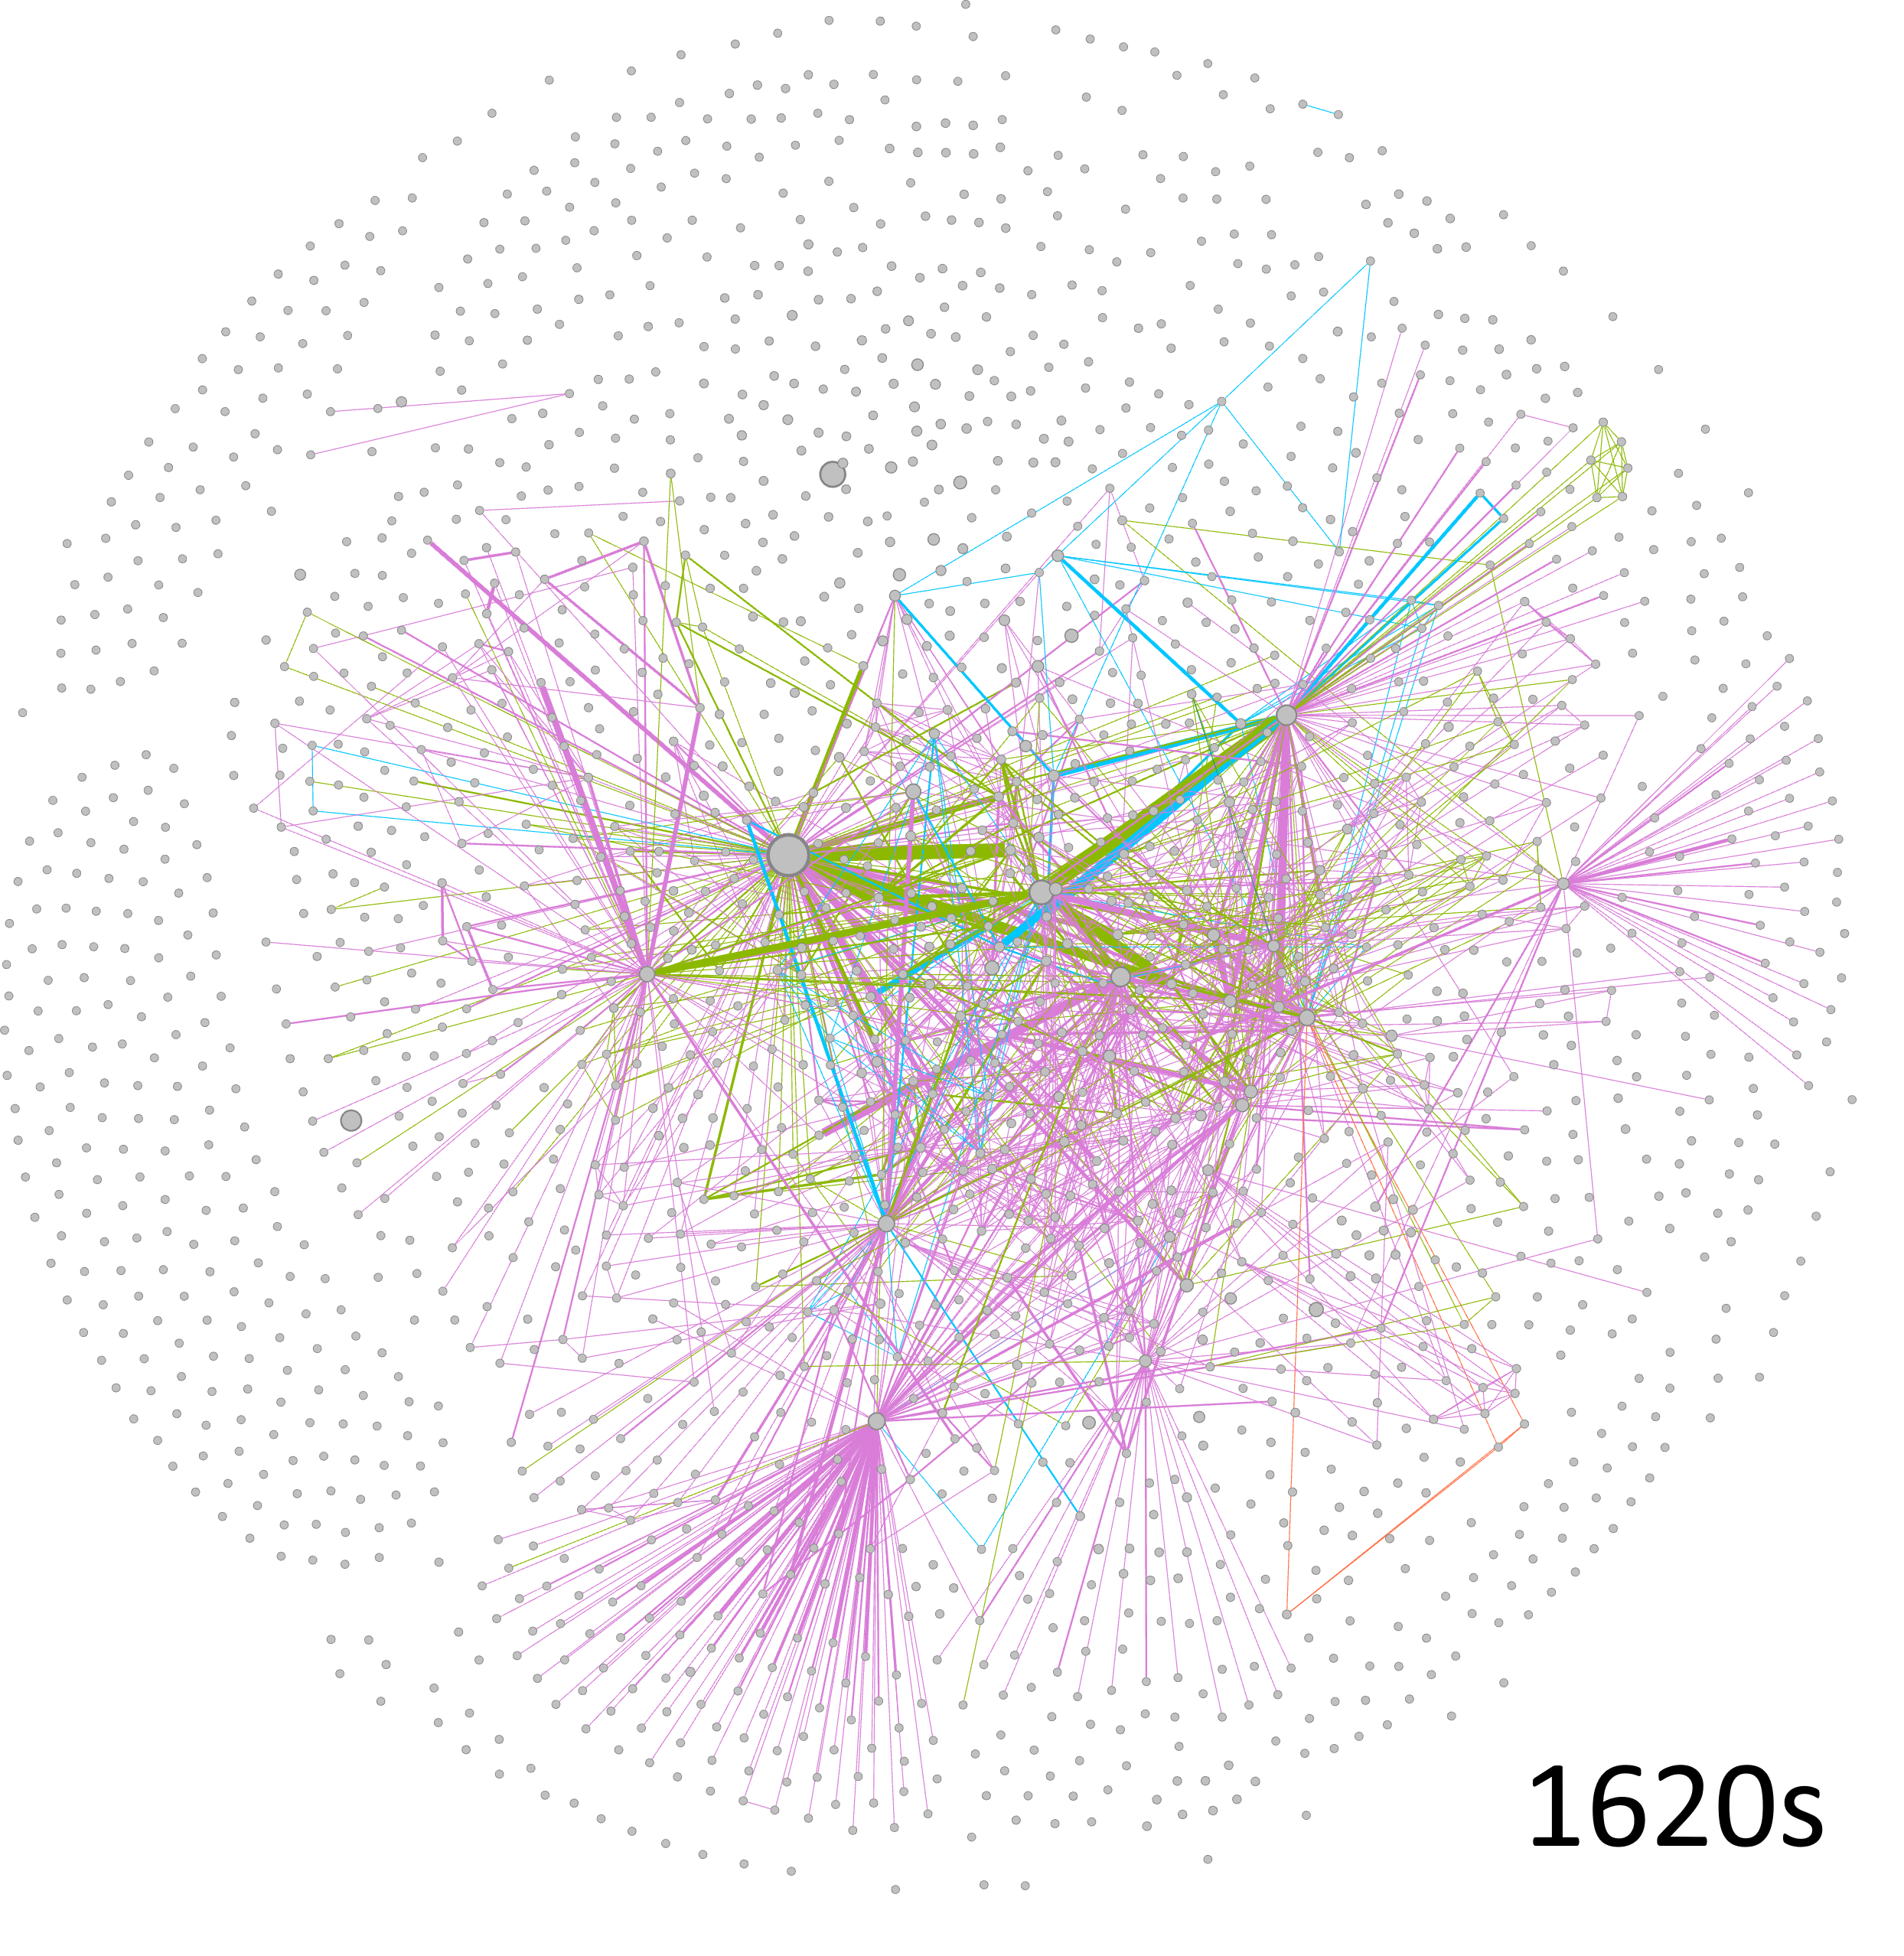
\includegraphics[scale=0.4]{graph/People_1620s.png}
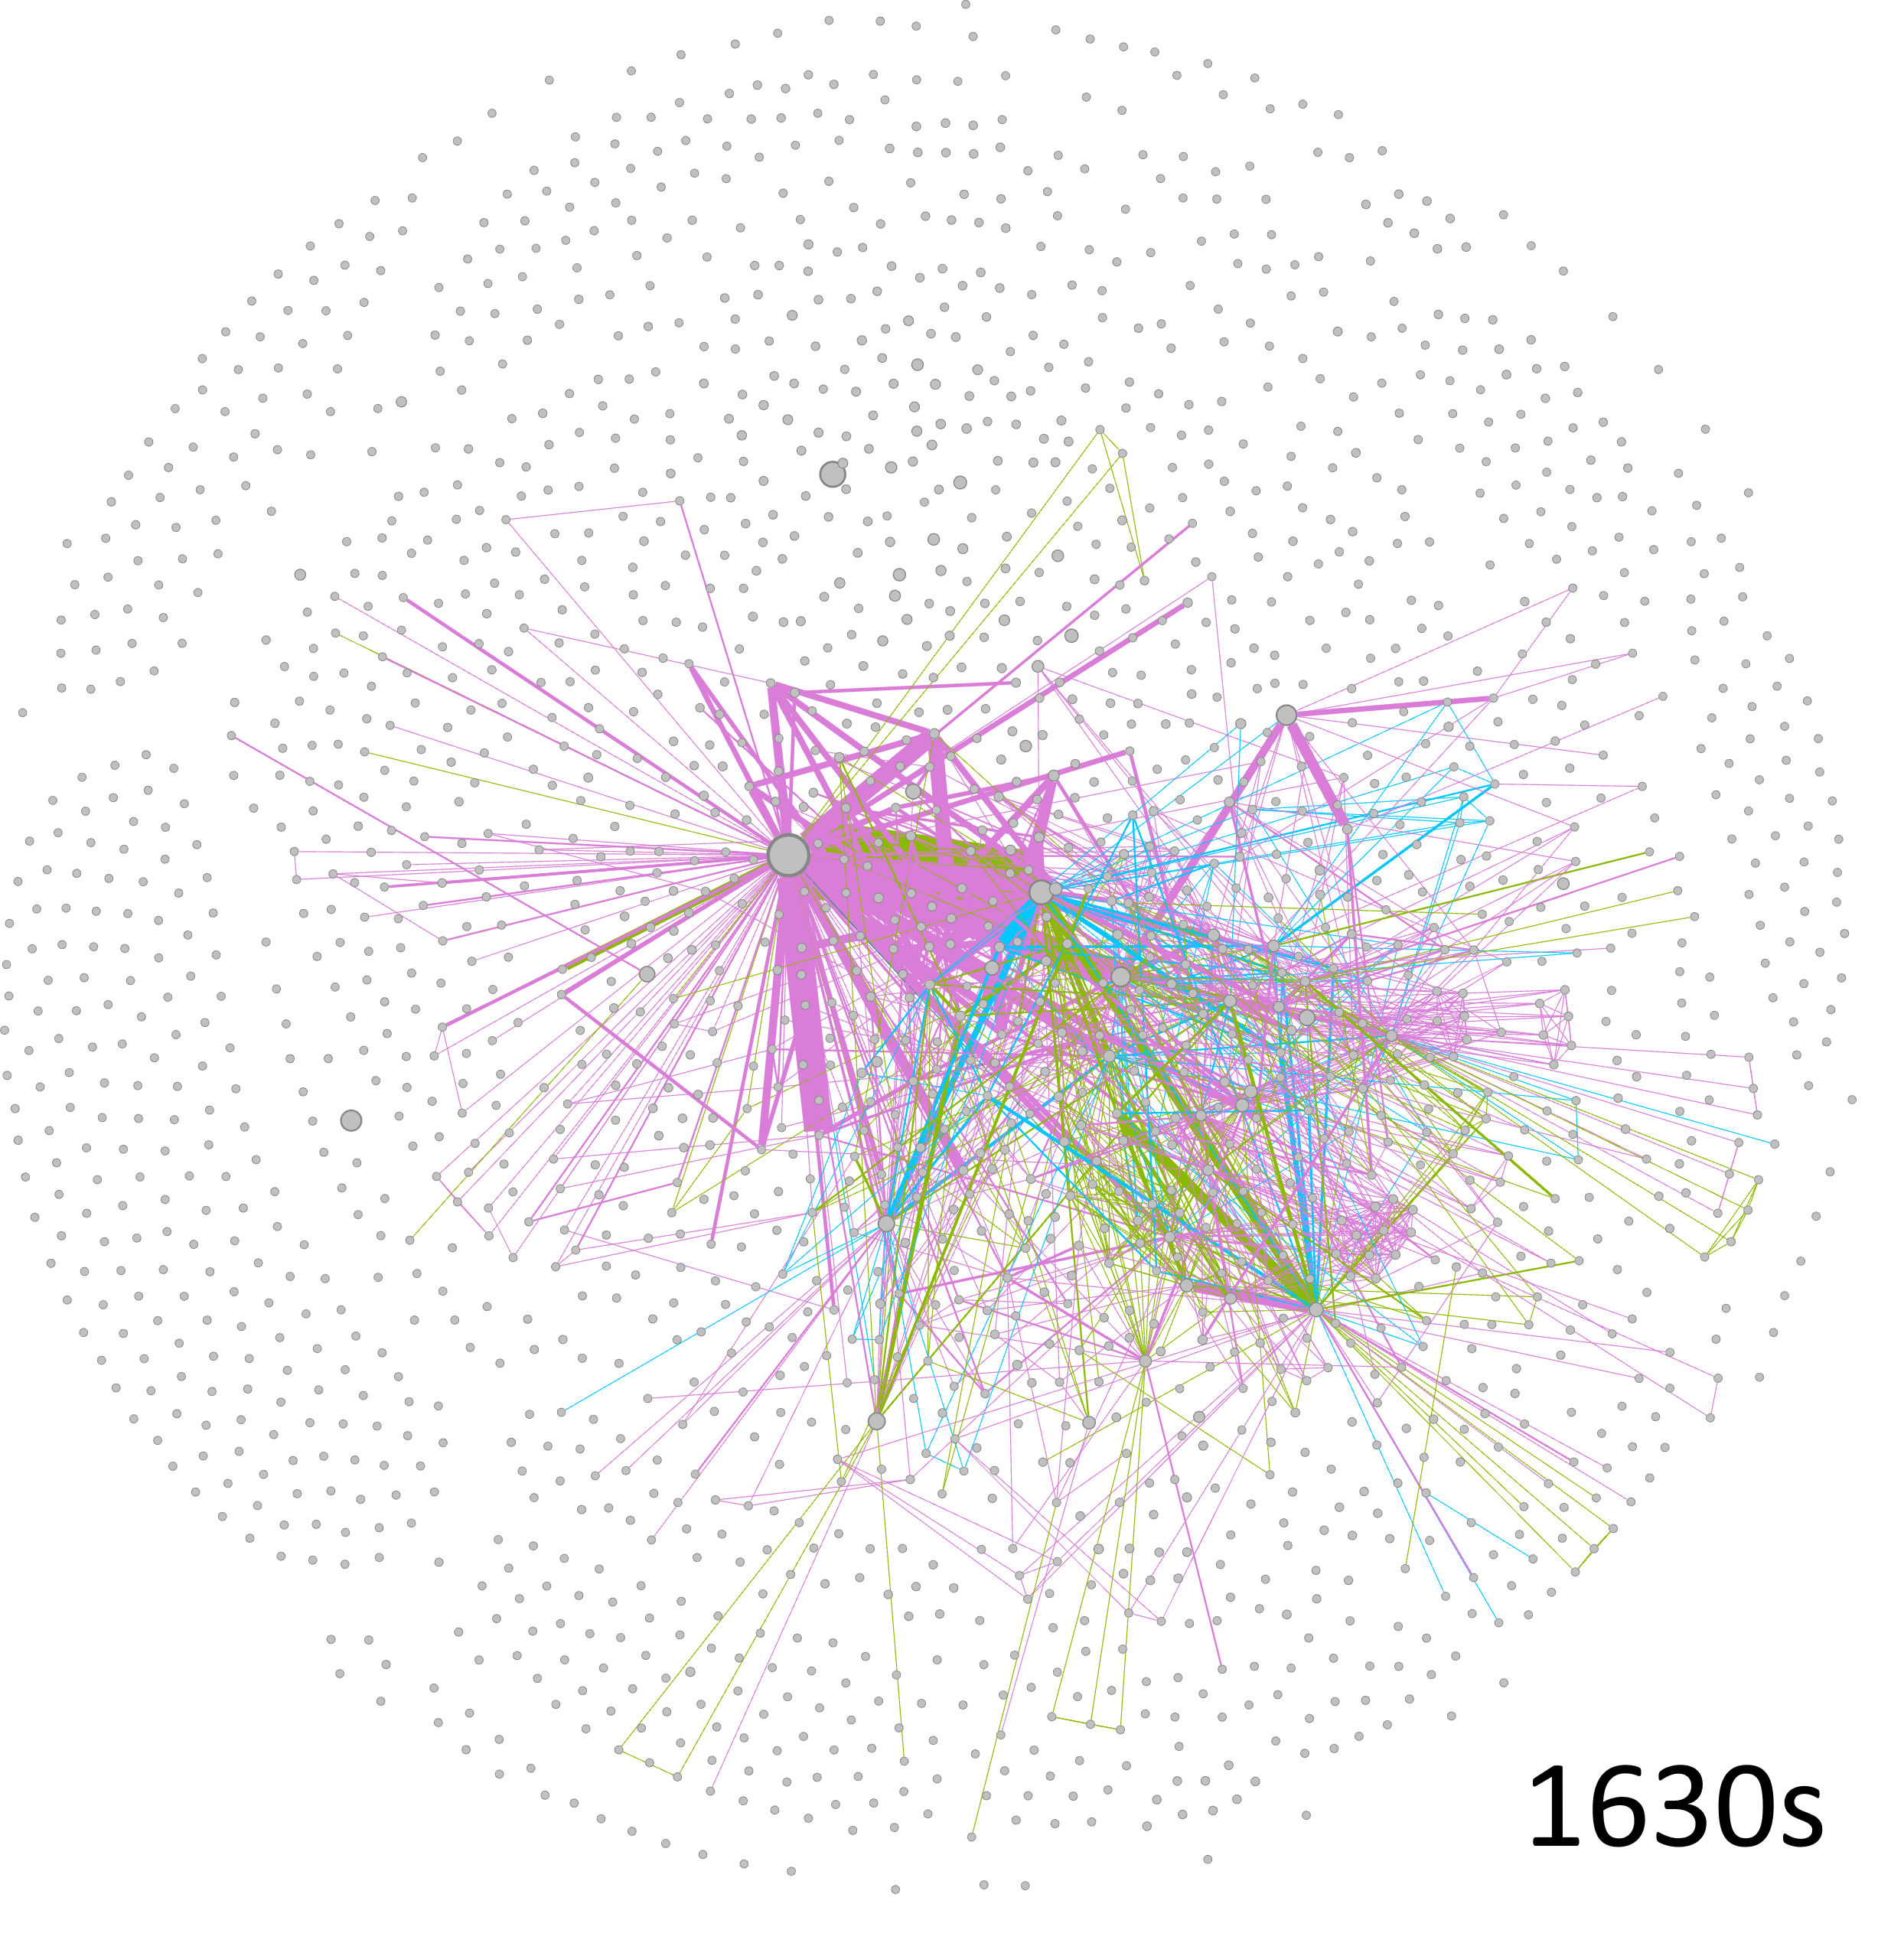
\includegraphics[scale=0.4]{graph/People_1630s.png}
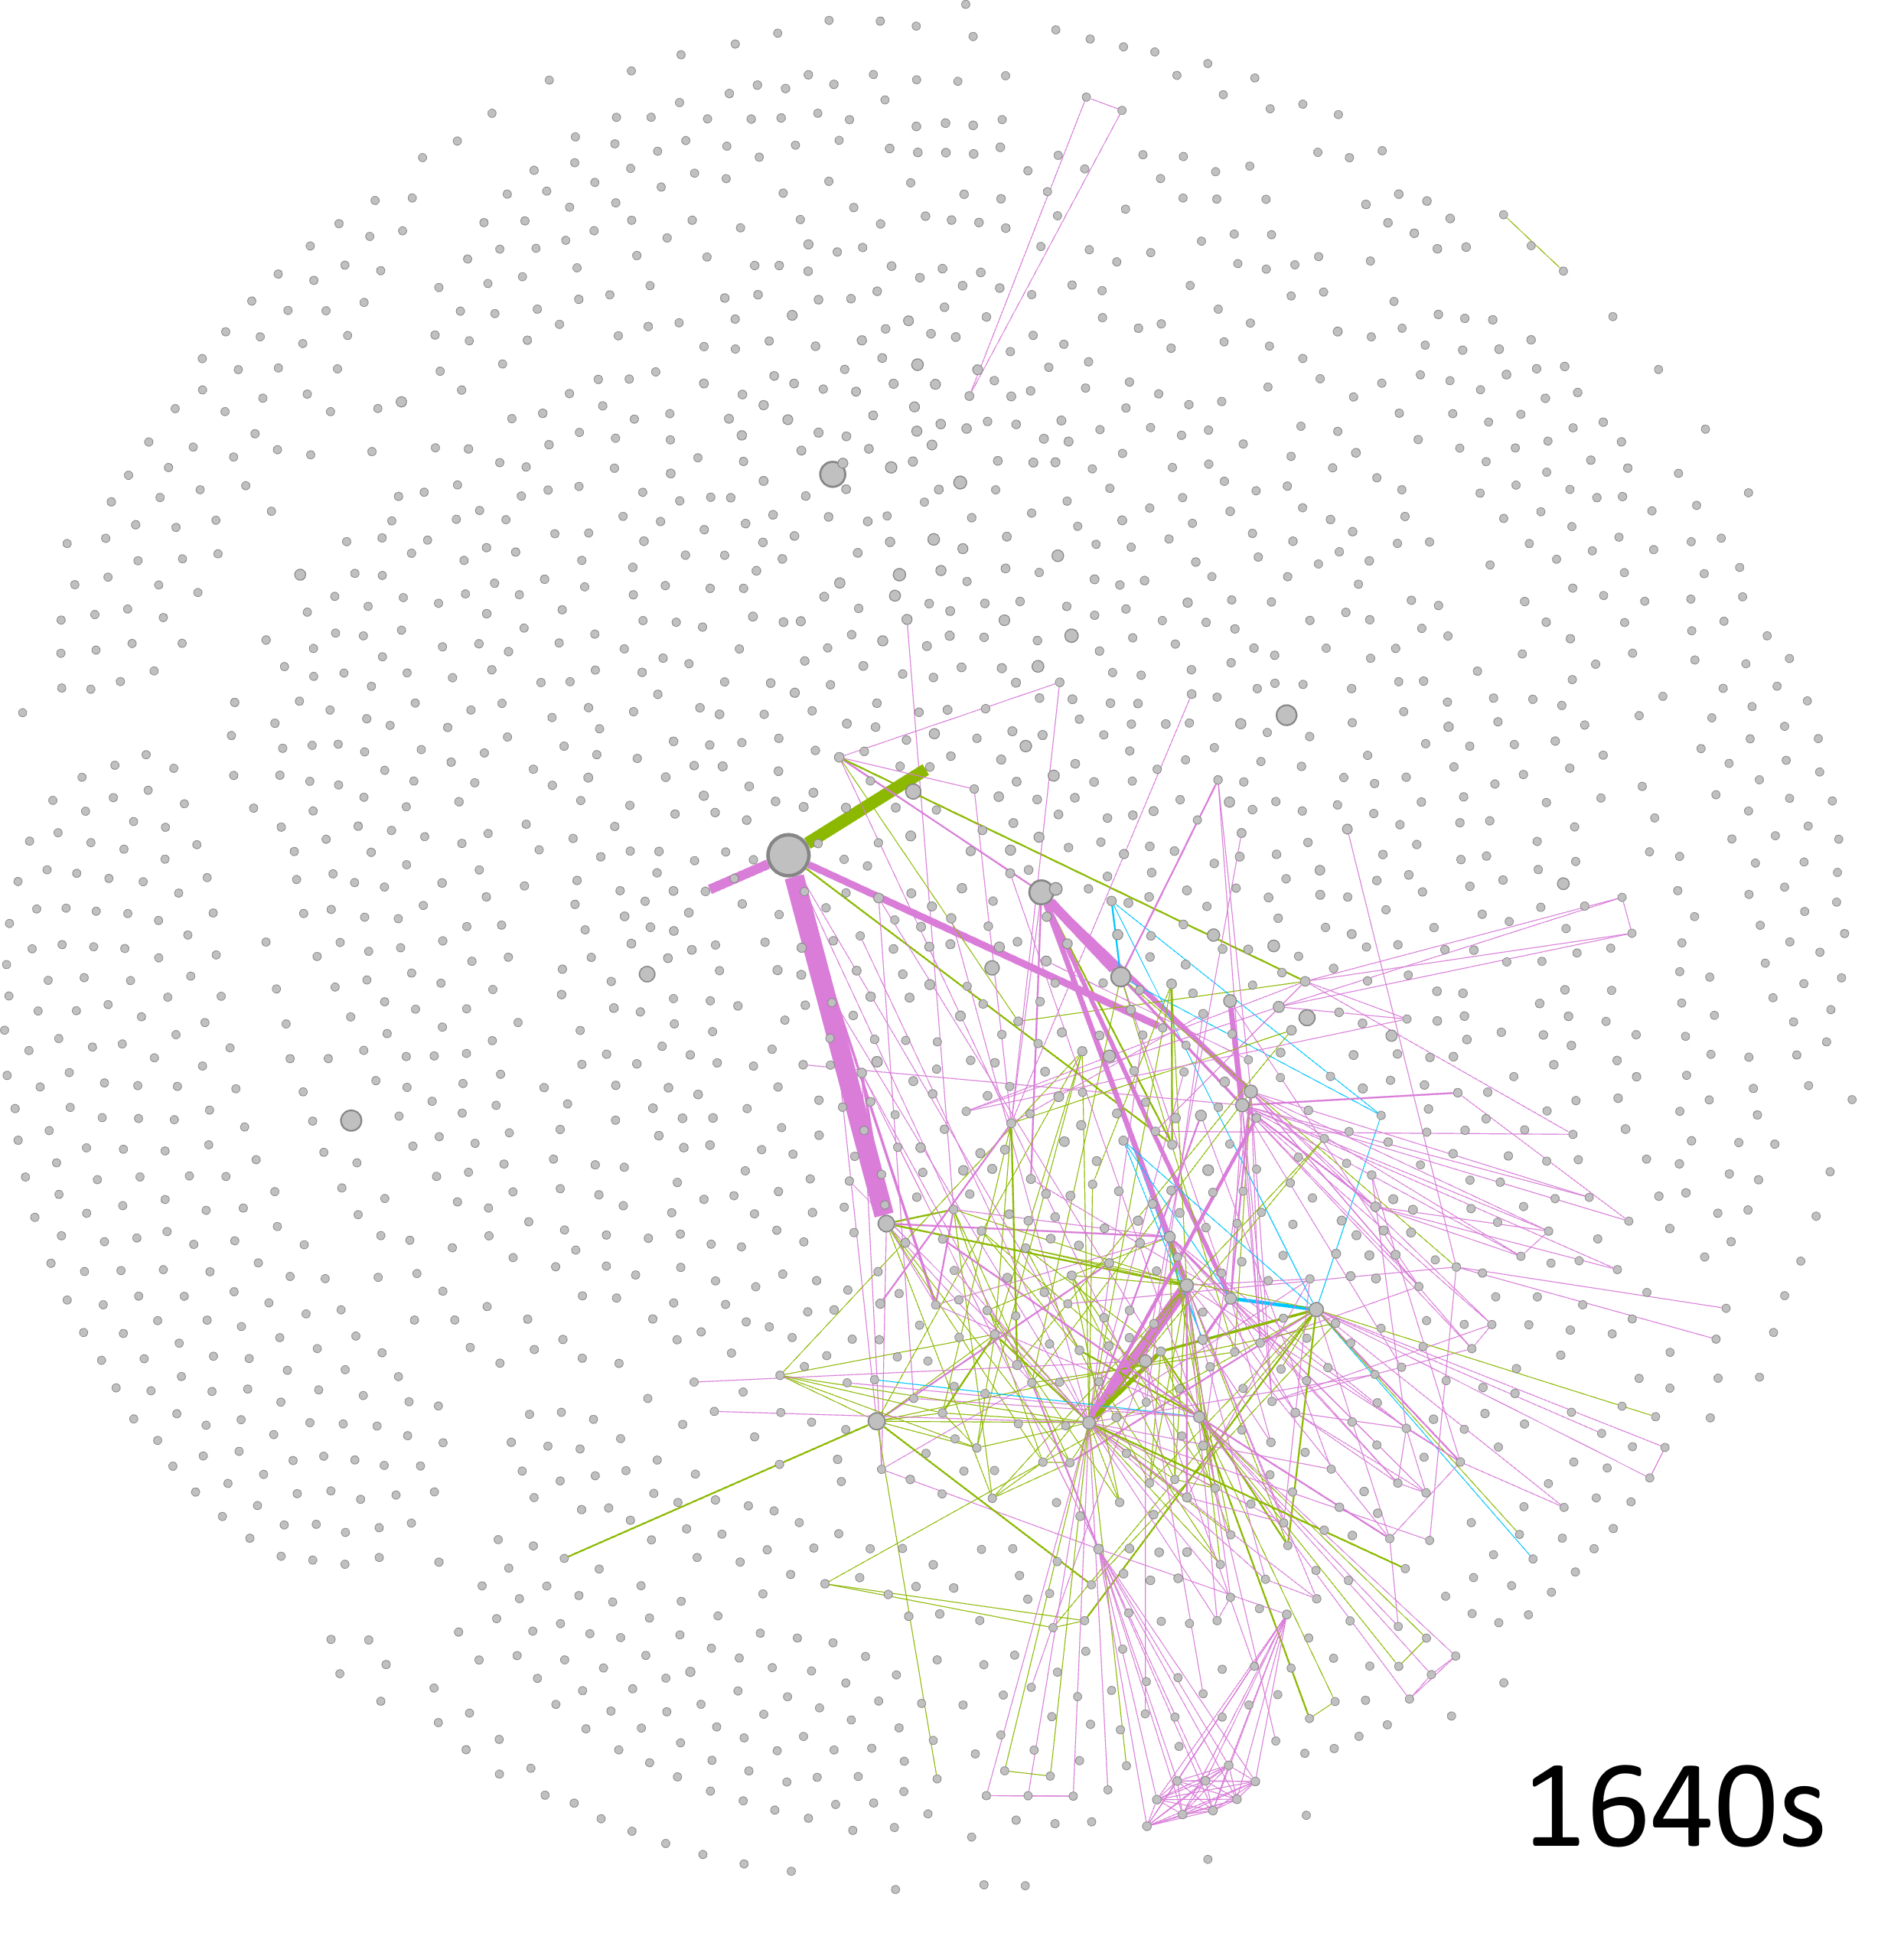
\includegraphics[scale=0.4]{graph/People_1640s.png}
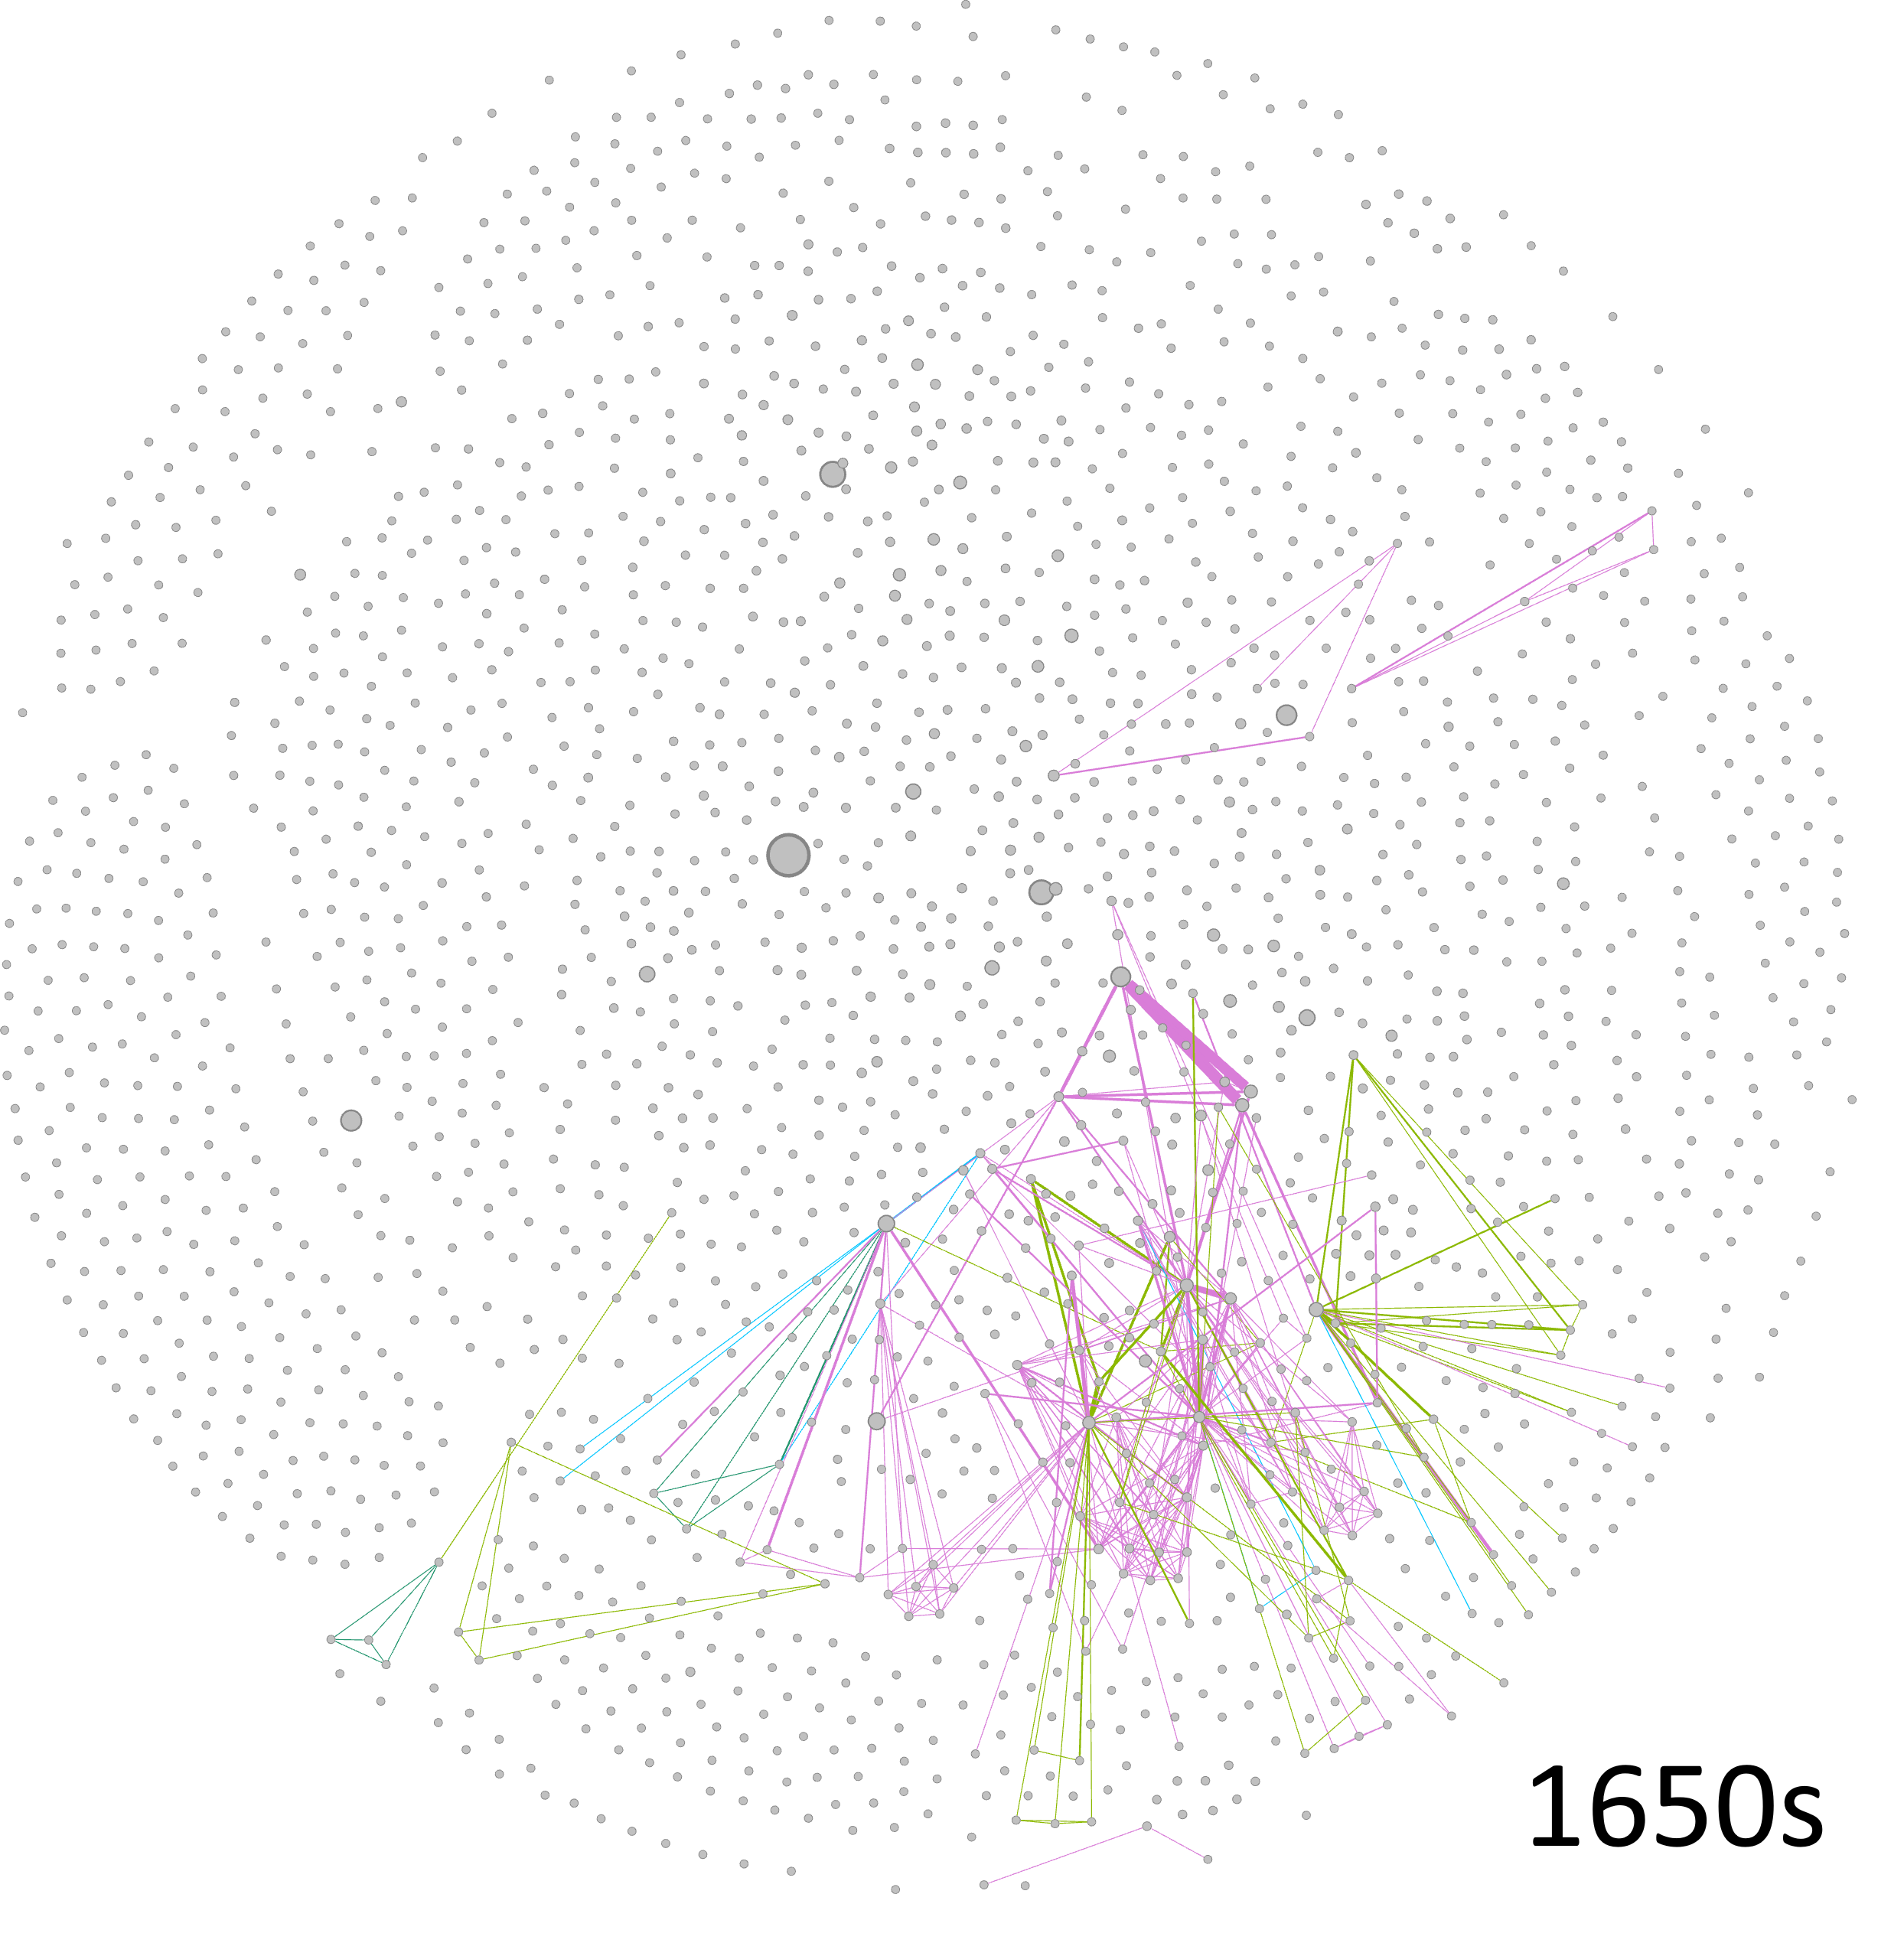
\includegraphics[scale=0.4]{graph/People_1650s.png}
\caption{Trend of the People Network after the 1600s}
\label{fig:peoNetAfter1600}
\end{figure}

In Figure \ref{fig:peoNetAfter1600}, we can observe the rise of English and Latin publications after the 1600s and the decline of the industry after the 1630s. The dominance of Latin publications during the 1610s and 1630s marks the peak of the Douai publishing industry. However, upon closer examination of the Network in the 1600s, English publications seem to be more well-connected to each other than Latin publications, indicating that the rising of English might have occurred slightly earlier than that of Latin in the industry. As mentioned in section \ref{languages}.1, the dynamics of English publications can represent the activities of English Catholics, this leads to the assumption that, in the second phase (the 1600s-1630s) of the development of the Douai publishing industry, The rise of English Catholics’ activities at the beginning triggered the later blooming of the industry.

We can justify the assumption with further calculation. By computing the extent of the connection of a node to other active nodes, Eigenvector Centrality can identify how influential a node is in the Network (Carrington \& Scott, 2011; Wasserman \& Faust, 1994). From Figure \ref{fig:eigenTrend} we can observe that the average Eigenvector Centrality of people involved in English publications suppressed the Centrality of people involved in the other two major languages (Latin and French) right before the industry height in the 1610s, implicating the triggering of the industry by the English Catholics.

\begin{figure}[H]
\centering
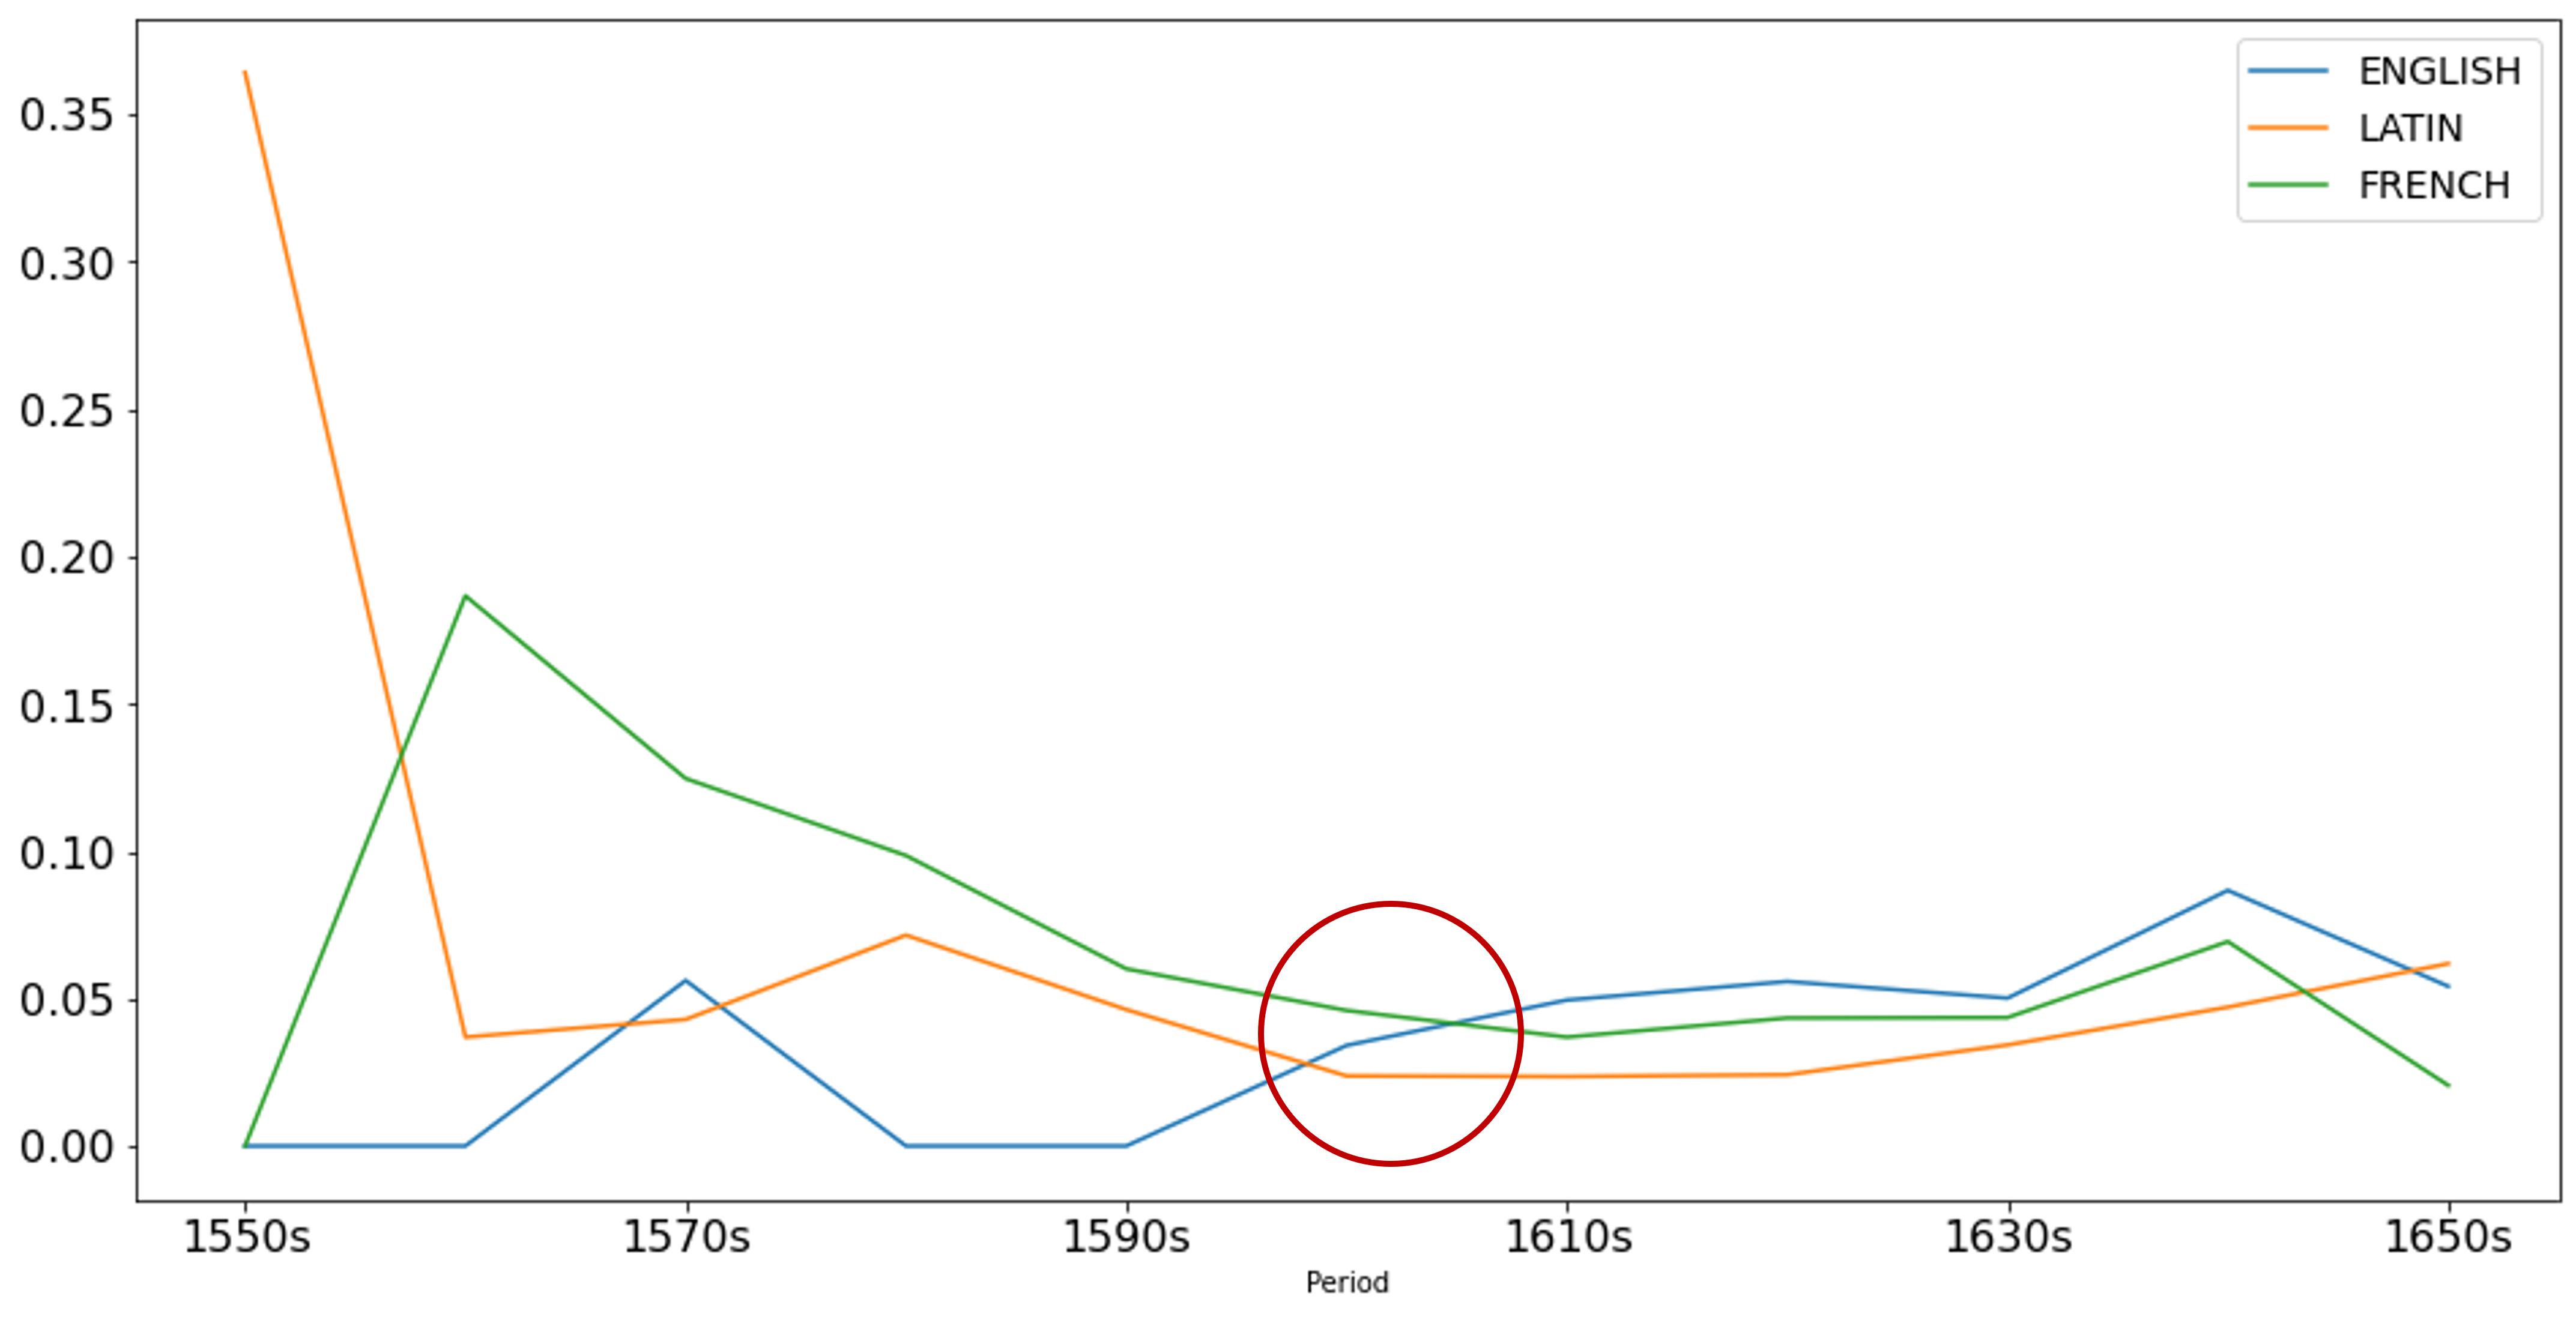
\includegraphics[scale=0.4]{graph/Trend of Average Eigenvector Centrality.png}
\caption{Trend of Average Eigenvector Centrality}
\label{fig:eigenTrend}
\end{figure}

Furthermore, we can conduct a statistical analysis to gain stronger evidence of the influence of English Catholics. In Table \ref{tab:eigenCross} we compare the average Eigenvector Centrality of nodes involved and not involved in English Publications by decades. The result shows that people who were involved in English publications had significantly higher (p-value $< 0.05$ in t-test) means of Eigenvector Centrality between the 1610s and 1640s, indicating that they were more influential during the peak of the industry. Since the dynamic of English publications can represent the activities of English Catholics, the result can be evident that it was English Catholics who were guiding the industry.

\begin{table}[H]
\centering
\caption{Cross Table of Average Eigenvector Centrality and Period}
\label{tab:eigenCross}
\begin{tabular}{llccccl}
 & \multicolumn{1}{c|}{\textbf{}}       & \multicolumn{2}{c}{\textbf{English}}                                                          & \multicolumn{2}{c}{\textbf{Non-English}}                 &  \\ \cline{2-6}
 & \multicolumn{1}{c|}{\textbf{Period}} & \multicolumn{1}{c|}{\textit{\textbf{n\tablefootnote{Number of who participated in English publications in this decade.}}}} & \multicolumn{1}{c|}{\textbf{Mean}}                 & \multicolumn{1}{c|}{\textit{\textbf{n\tablefootnote{Number of nodes who did not participate in English publications in this decade.}}}} & \textbf{Mean} &  \\ \cline{2-6}
 & \multicolumn{1}{l|}{1600s}           & \multicolumn{1}{c|}{\textit{52}}         & \multicolumn{1}{c|}{0.0341}                        & \multicolumn{1}{c|}{\textit{447}}        & 0.0245        &  \\
 & \multicolumn{1}{l|}{1610s}           & \multicolumn{1}{c|}{\textit{51}}         & \multicolumn{1}{c|}{{\color[HTML]{CB0000} 0.0495}} & \multicolumn{1}{c|}{\textit{540}}        & 0.0198        &  \\
 & \multicolumn{1}{l|}{1620s}           & \multicolumn{1}{c|}{\textit{45}}         & \multicolumn{1}{c|}{{\color[HTML]{CB0000} 0.0558}} & \multicolumn{1}{c|}{\textit{588}}        & 0.0208        &  \\
 & \multicolumn{1}{l|}{1630s}           & \multicolumn{1}{c|}{\textit{58}}         & \multicolumn{1}{c|}{{\color[HTML]{CB0000} 0.0502}} & \multicolumn{1}{c|}{\textit{366}}        & 0.0272        &  \\
 & \multicolumn{1}{l|}{1640s}           & \multicolumn{1}{c|}{\textit{12}}         & \multicolumn{1}{c|}{{\color[HTML]{CB0000} 0.0867}} & \multicolumn{1}{c|}{\textit{181}}        & 0.0433        &  \\
 & \multicolumn{1}{l|}{1650s}           & \multicolumn{1}{c|}{\textit{13}}         & \multicolumn{1}{c|}{0.0542}                        & \multicolumn{1}{c|}{\textit{132}}        & 0.0418        &  \\ \hline
\multicolumn{7}{l}{* {\color[HTML]{CB0000} Red numbers} are significantly higher.\tablefootnote{By t-test. 1610s: t=-6.05, p=2.63e-9; 1620s: t=-7.31, p=8.00e-13, 1630s: t=-4.38, p=1.52e-5; 1640s: t=-2.67, p=0.008.}}                                                                                                                                
\end{tabular}
\end{table}

Scholars (Soetaert \& Soen, 2020a; Soetaert \& Wyffels, 2021) suggest that the rising of the Douai publishing industry could be thanks to the coming English Catholics starting to collaborate deeper with local industry players and participate in more kinds of languages, and metrics of Closeness Centrality and Density of the Network can show this phenomenon. We calculate the metrics of people involved in English publications, which again is representative of English Catholics’ activities. Closeness Centrality considers the shortest paths of a node to others, indicating how well-connected (well-collaborated) this node is to others (Carrington \& Scott, 2011; Wasserman \& Faust, 1994). Density computes the proportion of the actual edges in all possible edges of a Network, implying how inter-close this Network is (Carrington \& Scott, 2011; Wasserman \& Faust, 1994). Together with the two kinds of metrics, we can see how well people involved in English publications collaborated with the whole network (Closeness Centrality), and how close people involved in English were with each other (Density).

During the 1600s to 1630s, their average Closeness Centrality\footnote{The Closeness Centrality is computed based on all the nodes in the People Network to see their collaboration with the whole Network.} (Figure \ref{fig:avgClose}) reached the plateau and their inner Density\footnote{The Density only takes the nodes involved in English publications into account so that it won’t inaccurately calculate irrelevant edges.} (Figure \ref{fig:avgDen}) dropped to the trough, meaning that English Catholics preferred to connect outwardly with others rather than only internally in this period. These results provide evidence for historians’ statement that after 1600, English Catholics worked more with local industry experts and were involved more in languages other than English (Soetaert \& Soen, 2020a; Soetaert \& Wyffels, 2021), and this expansion led to the blossoming of the industry.

\begin{figure}[H]
\centering
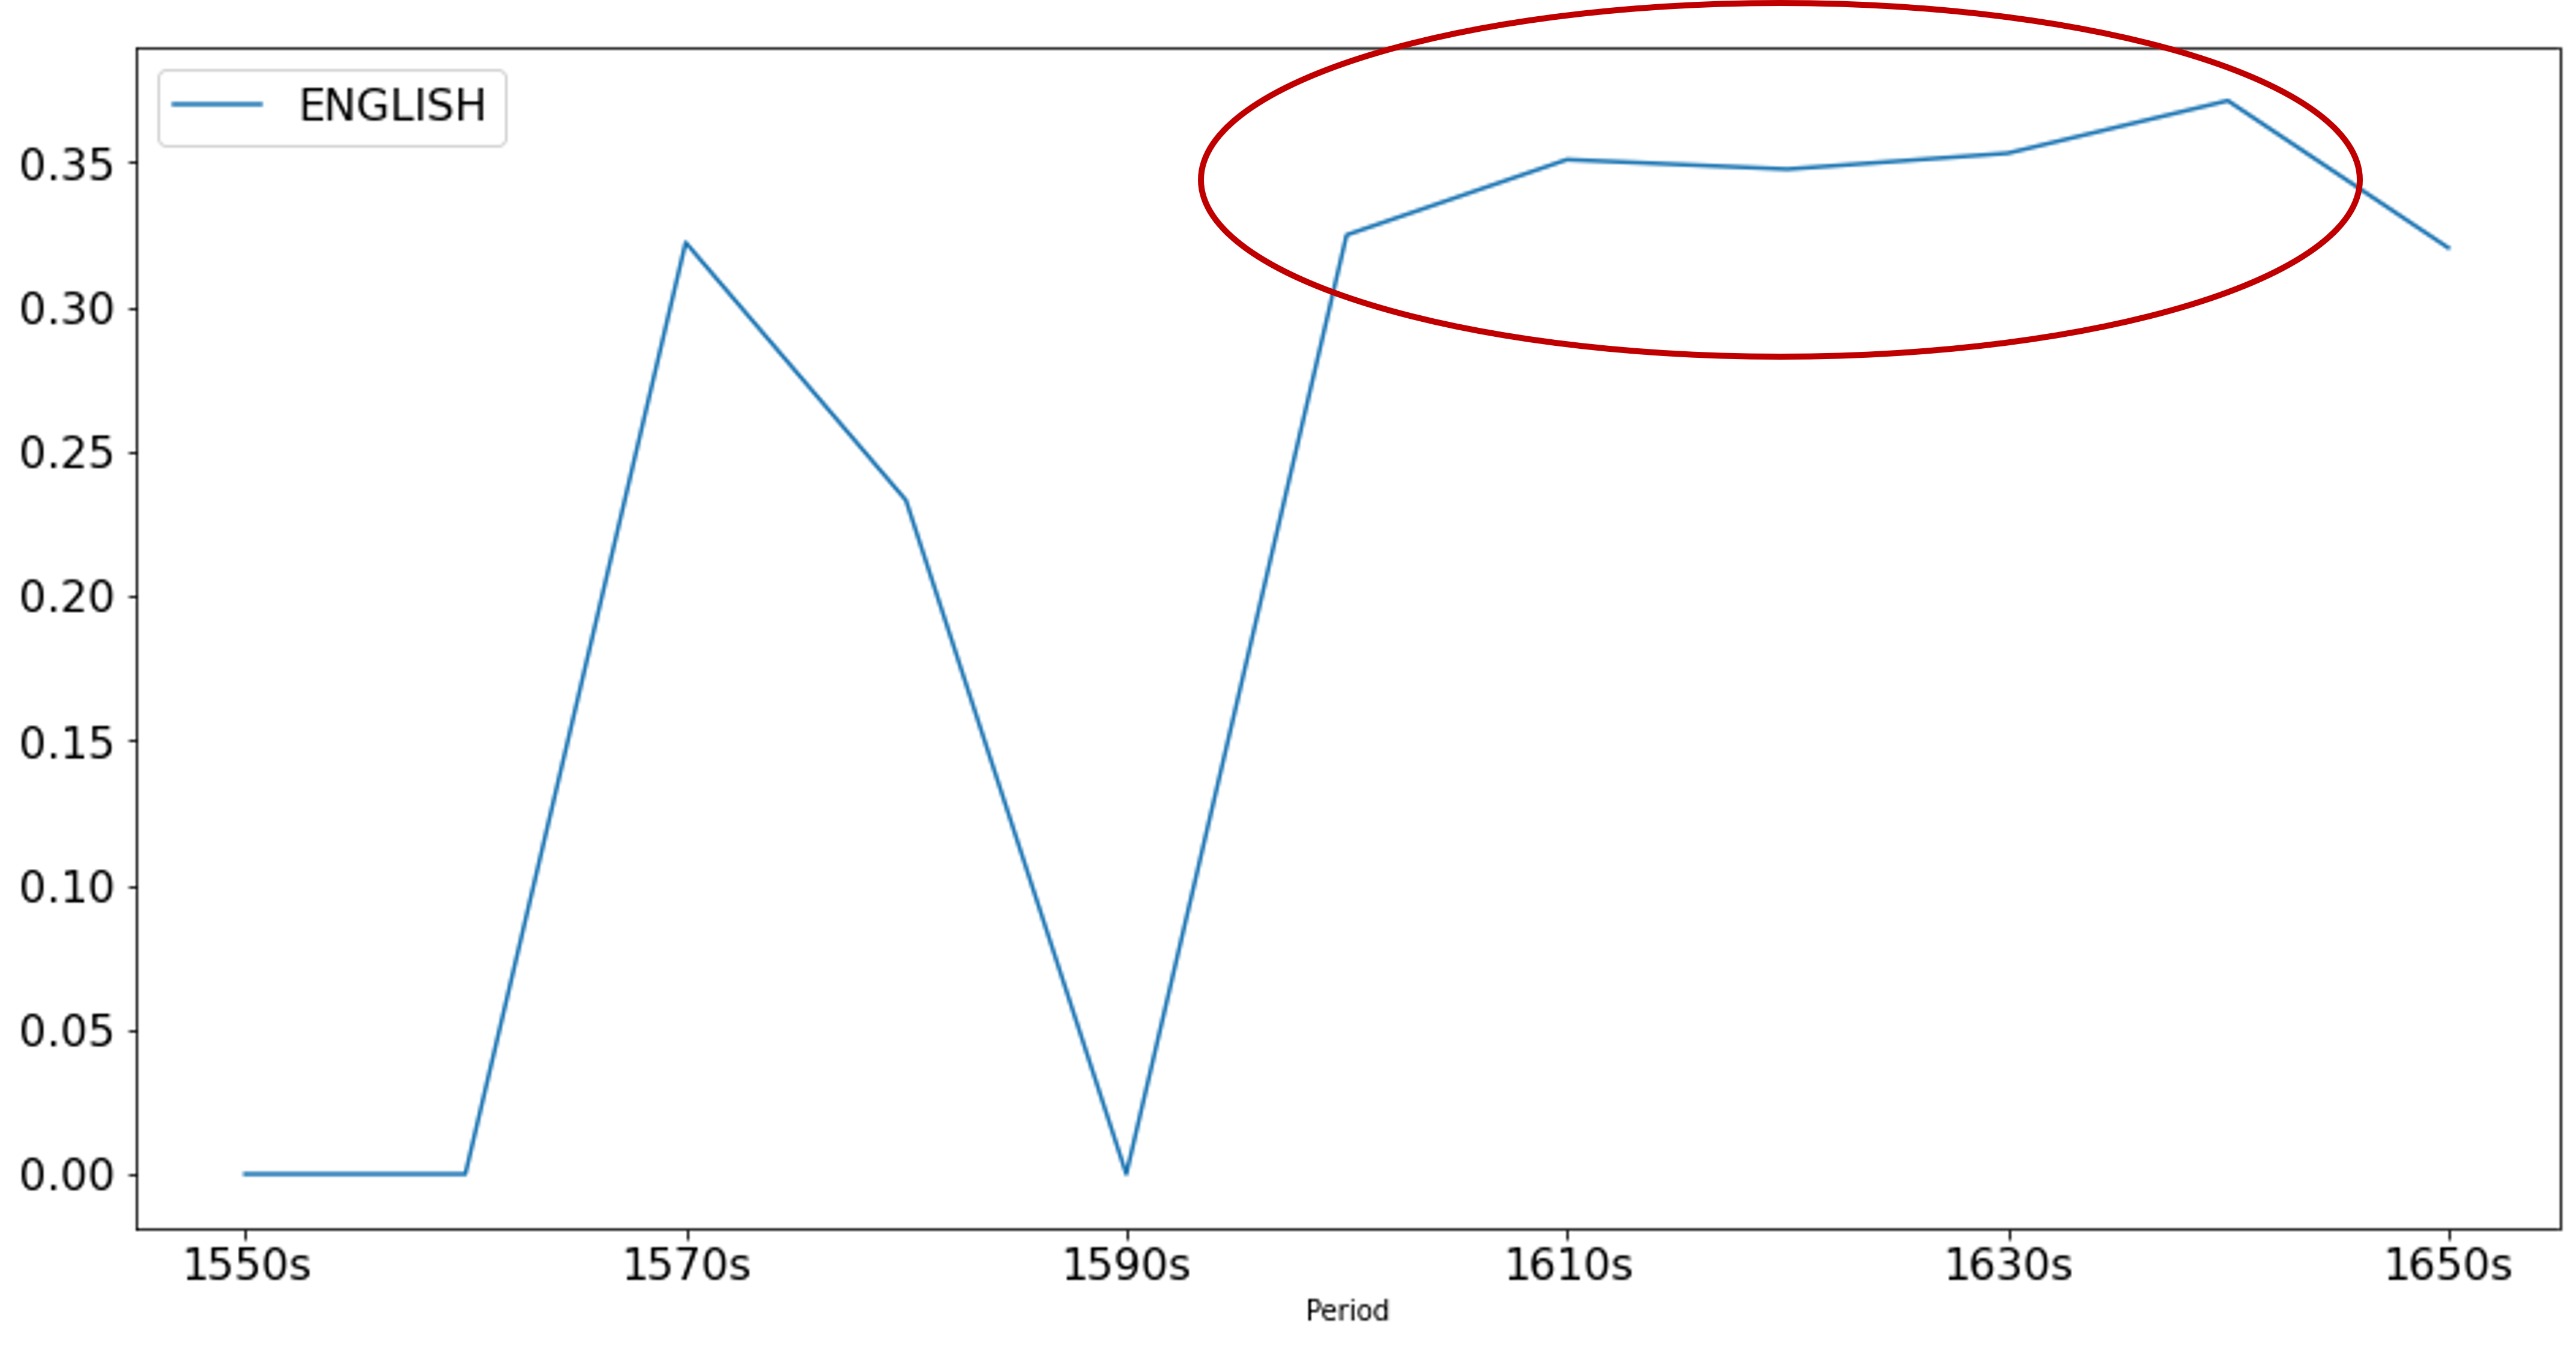
\includegraphics[scale=0.4]{graph/Average Closeness Centrality of English Publications.png}
\caption{Average Closeness Centrality of People Involved in English Publications}
\label{fig:avgClose}
\end{figure}

\begin{figure}[H]
\centering
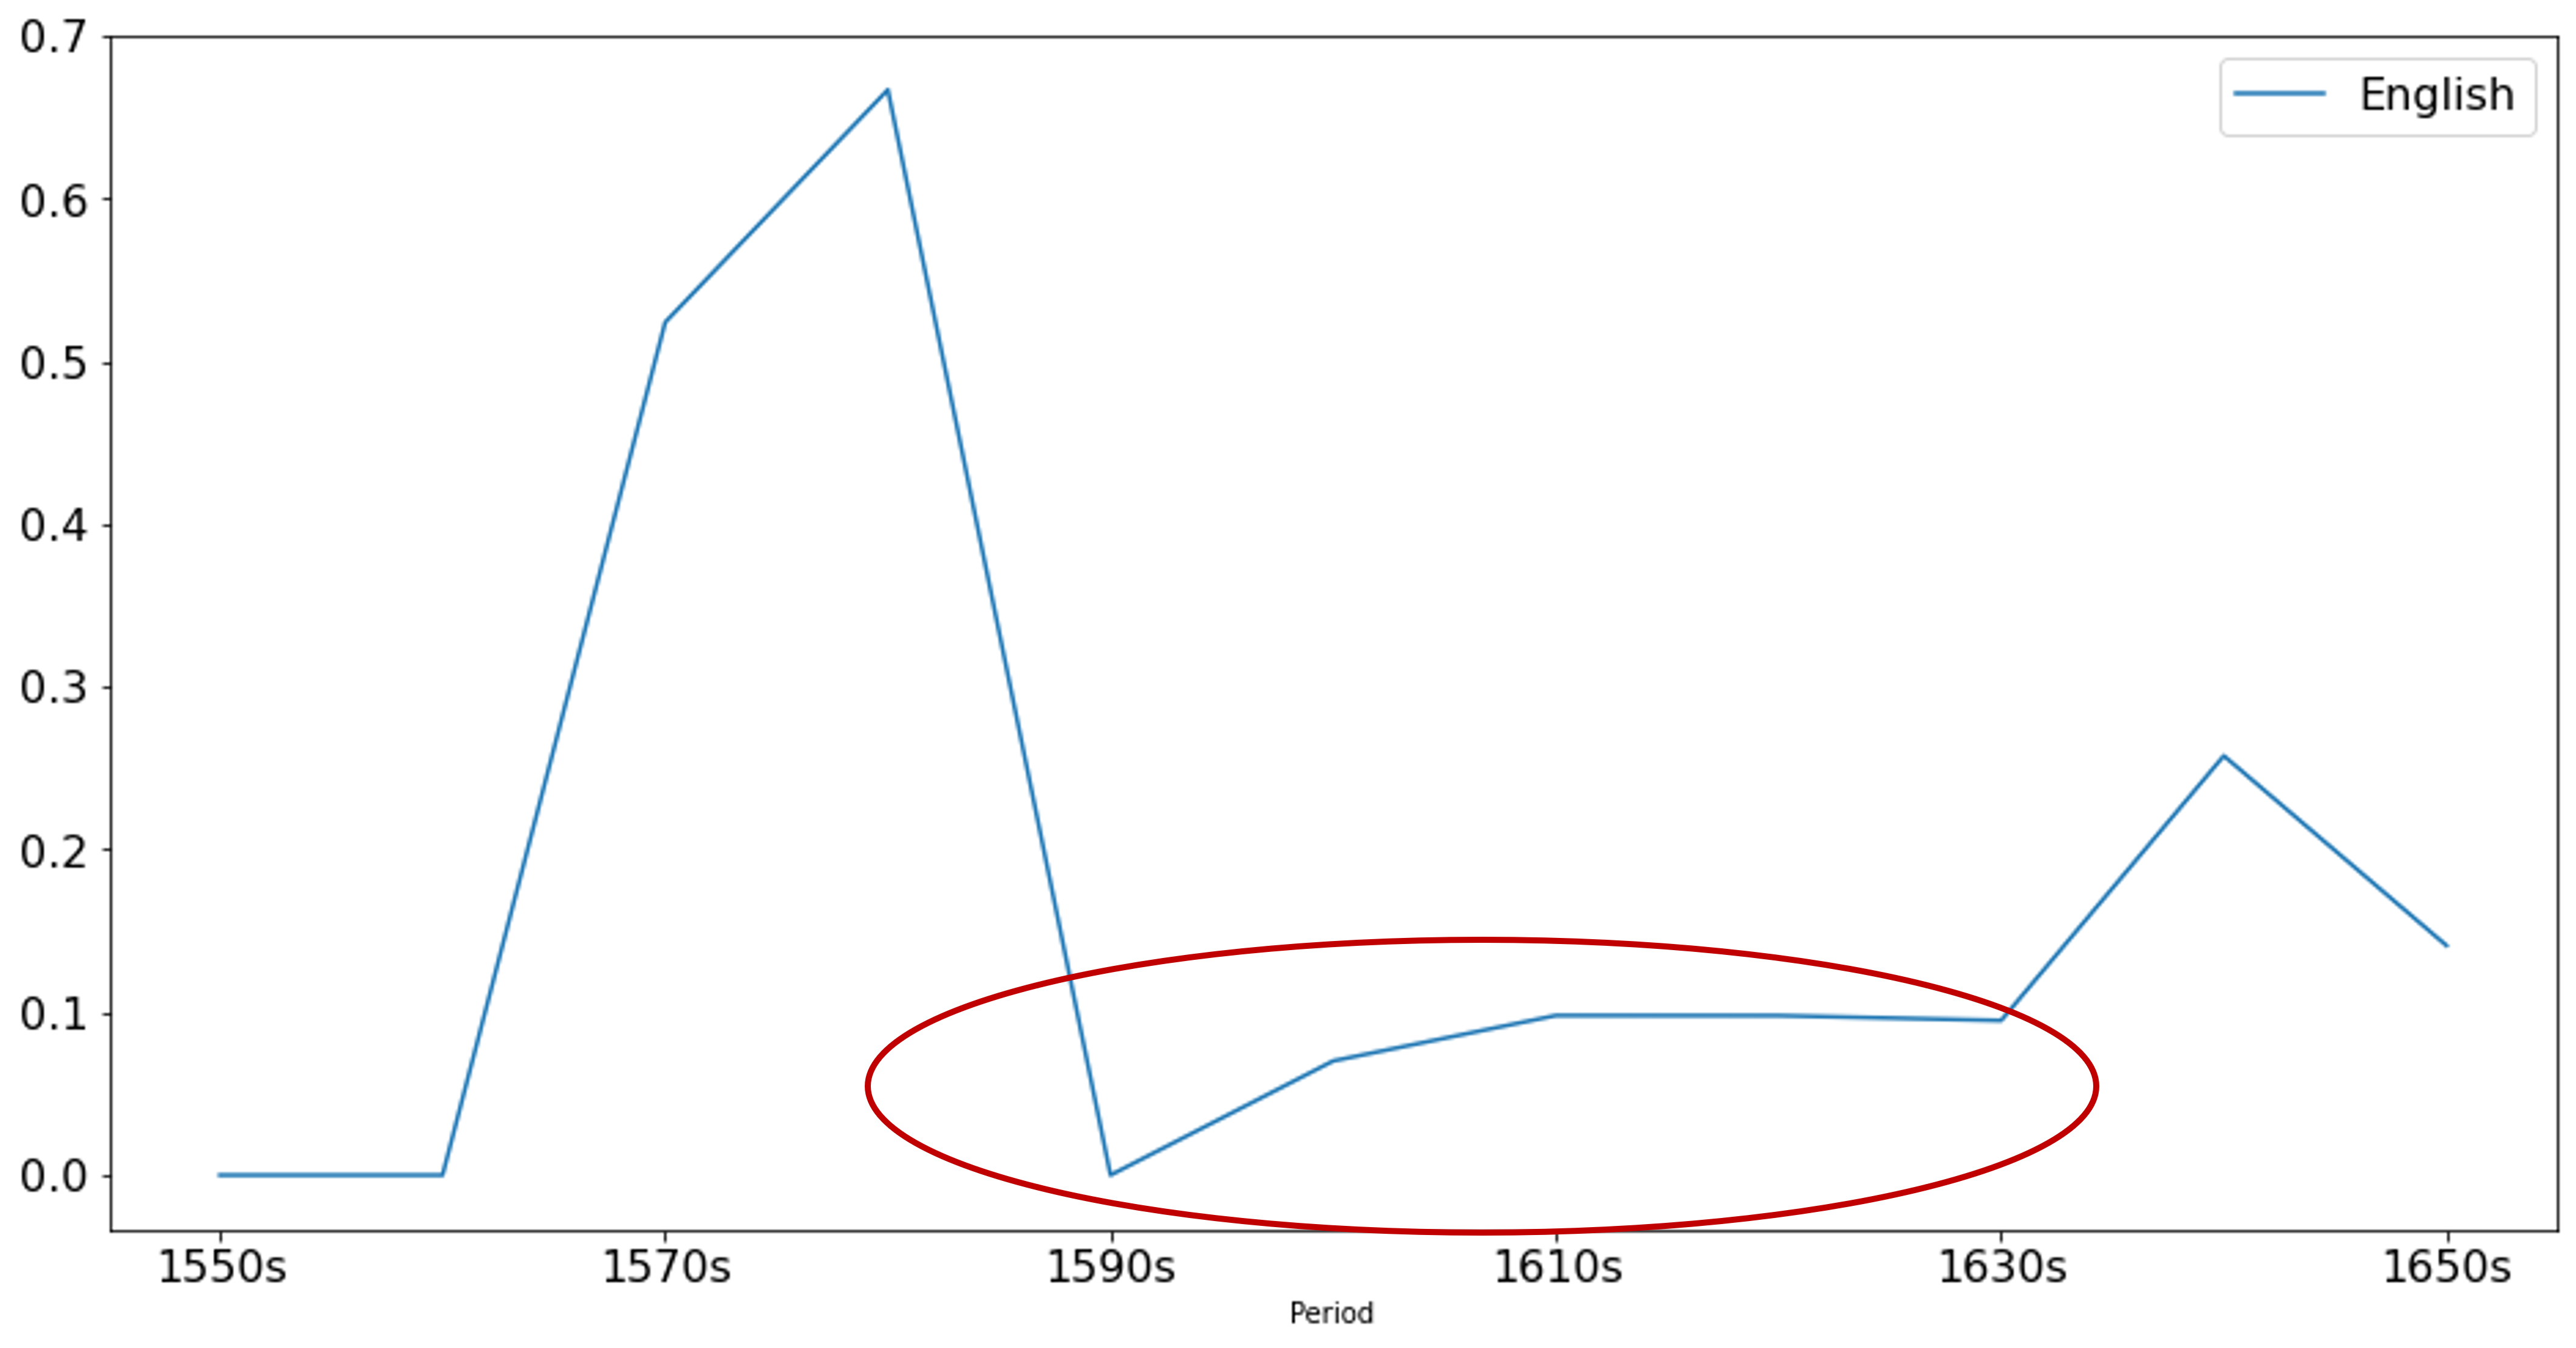
\includegraphics[scale=0.4]{graph/Average Density of English Publications.png}
\caption{Density of People Involved in English Publications}
\label{fig:avgDen}
\end{figure}

\counterwithout{footnote}{chapter}
\chapter{Influencers in the Industry}
\label{influencers}
In the previous chapter, by using the dynamic of the usage of language, we portrayed an overview of the publishing industry in Douai and how the English Catholics influenced it. In this chapter, we investigate the Network at an individual level. The Network structure introduced in the previous chapter is preserved for further investigation but with different annotations, and influencers’ participation in the Network is illustrated.

\section{Influential Individuals and Printing Houses}
From Chapter \ref{languages}, we have already realised the decisive participation of English Catholics in the publishing industry. However, what role did they usually play in the process of publishing? By computing the proportion of people's roles and comparing them between regions (Figure \ref{fig:regionXRole}\footnote{Since people can participate as several roles, the sum of each proportion is not exactly 1.0.}), we can observe that individuals from Britain, most likely English Catholics, tended to participate more in the content aspects (as compilers/editors/revisors) of publications. In contrast, local (Low Countries) people were more involved in the practical aspects (as printers/publishers). This tendency reaches statistical significance (p-values $< 0.05$ in z-test) (Table \ref{tab:regionXRole}) and illustrates the possible supply chain of the Douai publishing industry. English Catholics introduced and finalised text from authors and brought the text to the local printers/publishers for publishing.

\begin{table}[H]
\centering
\caption{Cross Table of Birth Region and Role (in proportion)}
\label{tab:regionXRole}
\begin{tabular}{lcccc}
\multicolumn{1}{l|}{}                        & \textbf{Britain}            & \multicolumn{1}{c|}{\textbf{Non-Britain}} & \textbf{Low}                & \textbf{Non-Low} \\ \hline
\multicolumn{1}{l|}{\textit{n\tablefootnote{Number of people from each region.}}}              & \textit{60}                 & \multicolumn{1}{c|}{\textit{343}}         & \textit{202}                & \textit{201}     \\ \hline
\multicolumn{1}{l|}{compiler/editor/revisor} & {\color[HTML]{CB0000} 0.22} & \multicolumn{1}{c|}{0.10}                 & 0.14                        & 0.10             \\
\multicolumn{1}{l|}{printer/publisher}       & 0.03                        & \multicolumn{1}{c|}{0.08}                 & {\color[HTML]{CB0000} 0.11} & 0.01             \\ \hline
\multicolumn{5}{l}{* {\color[HTML]{CB0000} Red numbers} are significantly higher than other groups.\tablefootnote{By proportional z-test. Compiler/editor/revisor: Britain vs. non-Britain: z=2.44, p=0.01; printer/publisher: Low Countries vs. non-Low Countries: z=3.91, p=9.20e-5}}                                                                               
\end{tabular}
\end{table}

\begin{figure}[H]
\centering
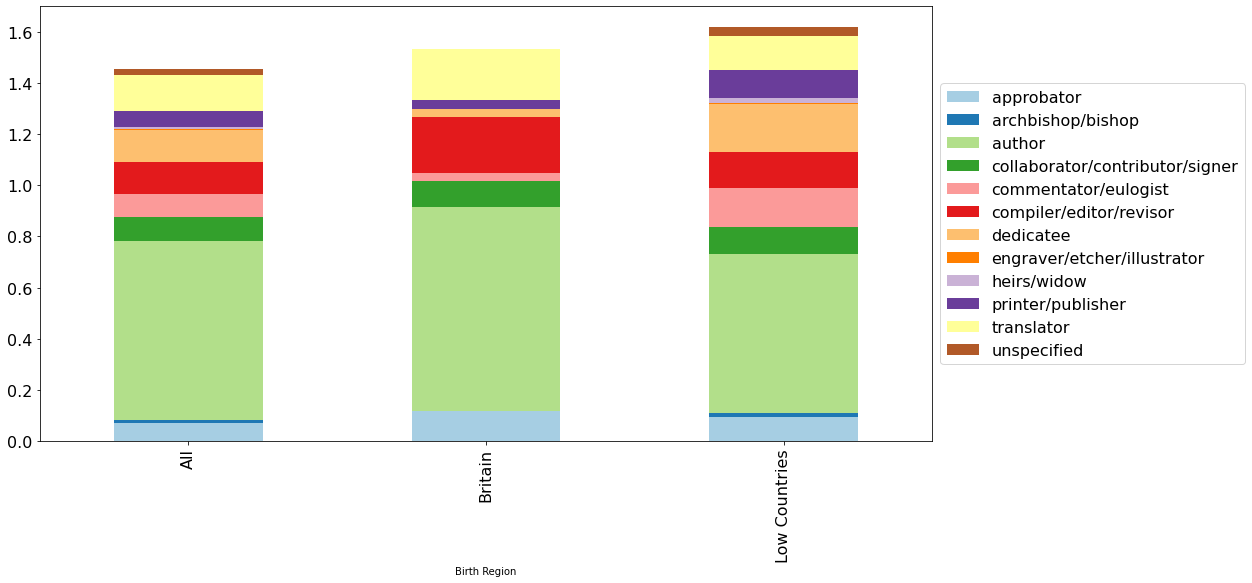
\includegraphics[scale=0.35]{graph/Stack Chart of Birth Region and Role.png}
\caption{Stack Chart of Birth Region and Role}
\label{fig:regionXRole}
\end{figure}

This could explain why the most influential person in this Network is a printer and publisher from Low Countries, Balthazar I Bellère. He originated from Antwerp but moved to Douai for his publishing career (Soetaert et al., 2022a). With a Degree of 585, he had connections with 30\% of the people (Degree Centrality = 0.3) in this Network. Having the highest Centrality in Eigenvector and Betweenness not only shows his influence on the industry but also aligns with historian’s observations (Soetaert \& Soen, 2020a; Soetaert \& Wyffels, 2021) that lots of industry experts, such as editors and translators, were able to be connected through him since Betweenness Centrality measures how often a node acts as an intermediate between other nodes (Carrington \& Scott, 2011; Wasserman \& Faust, 1994). In addition, having the highest Closeness Centrality and a relatively low Clustering Coefficient indicates the ability of the node to connect with various clusters in the Network rather than just staying within its own. This corresponds with the history that besides English, Balthazar I Bellère also collaborated a lot with other communities such as Flemish and Walloon (Soetaert \& Soen, 2020a).

Other people in the top 5 list, Jan I Bogart, Christine De Roovere and Pierre Auroy, are also printers/publishers who originated from Low Countries (Soetaert, 2020b; Soetaert et al., 2022b, 2023a). On the other hand, Georges Colveneere, a professor at the University of Douai, mainly served as an approbator in the industry (Soetaert \& Soen, 2020b).

\begin{table}[H]
\centering
\caption{Top 5 Degrees in the People Network}
\label{tab:top5Degree}
\resizebox{\textwidth}{!}{
\begin{tabular}{lccccc}
\multicolumn{1}{c|}{\textbf{Name}}                               & \textbf{Degree}            & \textbf{Betweenness}          & \textbf{Closeness}          & \textbf{Clustering}         & \textbf{Eigenvector}        \\ \hline
\multicolumn{1}{l|}{{\color[HTML]{303498} Balthazar I Bellère}}  & {\color[HTML]{303498} 585} & {\color[HTML]{303498} 0.3124} & {\color[HTML]{303498} 0.50} & {\color[HTML]{303498} 0.01} & {\color[HTML]{303498} 0.38} \\
\multicolumn{1}{l|}{{\color[HTML]{303498} Jan I Bogart}}         & {\color[HTML]{303498} 300} & {\color[HTML]{303498} 0.1165} & {\color[HTML]{303498} 0.41} & {\color[HTML]{303498} 0.03} & {\color[HTML]{303498} 0.18} \\
\multicolumn{1}{l|}{Georges Colveneere}                          & 282                        & 0.1330                        & 0.50                        & 0.04                        & 0.27                        \\
\multicolumn{1}{l|}{{\color[HTML]{303498} Christine De Roovere}} & {\color[HTML]{303498} 218} & {\color[HTML]{303498} 0.1752} & {\color[HTML]{303498} 0.41} & {\color[HTML]{303498} 0.00} & {\color[HTML]{303498} 0.05} \\
\multicolumn{1}{l|}{{\color[HTML]{303498} Pierre Auroy}}         & {\color[HTML]{303498} 211} & {\color[HTML]{303498} 0.0891} & {\color[HTML]{303498} 0.43} & {\color[HTML]{303498} 0.04} & {\color[HTML]{303498} 0.16} \\ \hline
\multicolumn{6}{l}{* {\color[HTML]{303498} Blue people} are printers/publishers who originated from Low Countries}                                                                                                                                                                                 
\end{tabular}
}
\end{table}

\pagebreak
Interestingly, the person from Britain who had the highest Degree is not an author or compiler/editor/revisor but also a printer/publisher, Laurence I Kellam. He came to Leuven to start his printing career in 1595 then eventually moved to Douai in 1603 (Soetaert et al., 2021). His son, Laurence II Kellam, who was likely born in Leuven, inherited his family’s printing business (Soetaert, 2020a) and became more influential in the industry than his father. They all had a higher Clustering Coefficient than the top 5 influencers in the industry, implying that they might interact more within a specific community, which was probably the English community according to their background.

\begin{table}[H]
\centering
\caption{Network Metrics of Laurence I Kellam and Laurence II Kellam}
\label{tab:kellamMetrics}
\resizebox{\textwidth}{!}{
\begin{tabular}{l|ccccc}
\multicolumn{1}{c|}{\textbf{Name}} & \textbf{Degree} & \textbf{Betweenness} & \textbf{Closeness} & \textbf{Clustering} & \textbf{Eigenvector} \\ \hline
Laurence II Kellam                 & 145             & 0.0481               & 0.05               & 0.41                & 0.12                 \\
Laurence I Kellam                  & 91              & 0.0207               & 0.06               & 0.40                & 0.09                
\end{tabular}
}
\end{table}

Scholars already observed that printers and publishers had a decisive influence on the development of the publishing industry in Douai (Soetaert, 2019a, 2014; Soetaert \& Soen, 2020a; Soetaert \& Wyffels, 2021), and the activities of printing houses were often used to describe the development of the industry. Therefore, it can be interesting to illustrate printing houses on the Network. To do this, several houses are identified\footnote{See Appendix \ref{app:printHouse}.} and they are categorised as “Low Countries” originated, or “Britain” originated based on the origin of their founders. From Figure \ref{fig:onlyPrint}, you can already notice the influence of these printing houses, especially the ones from the Low Countries since their connection stretches almost the entire Network.

\begin{figure}[H]
\centering
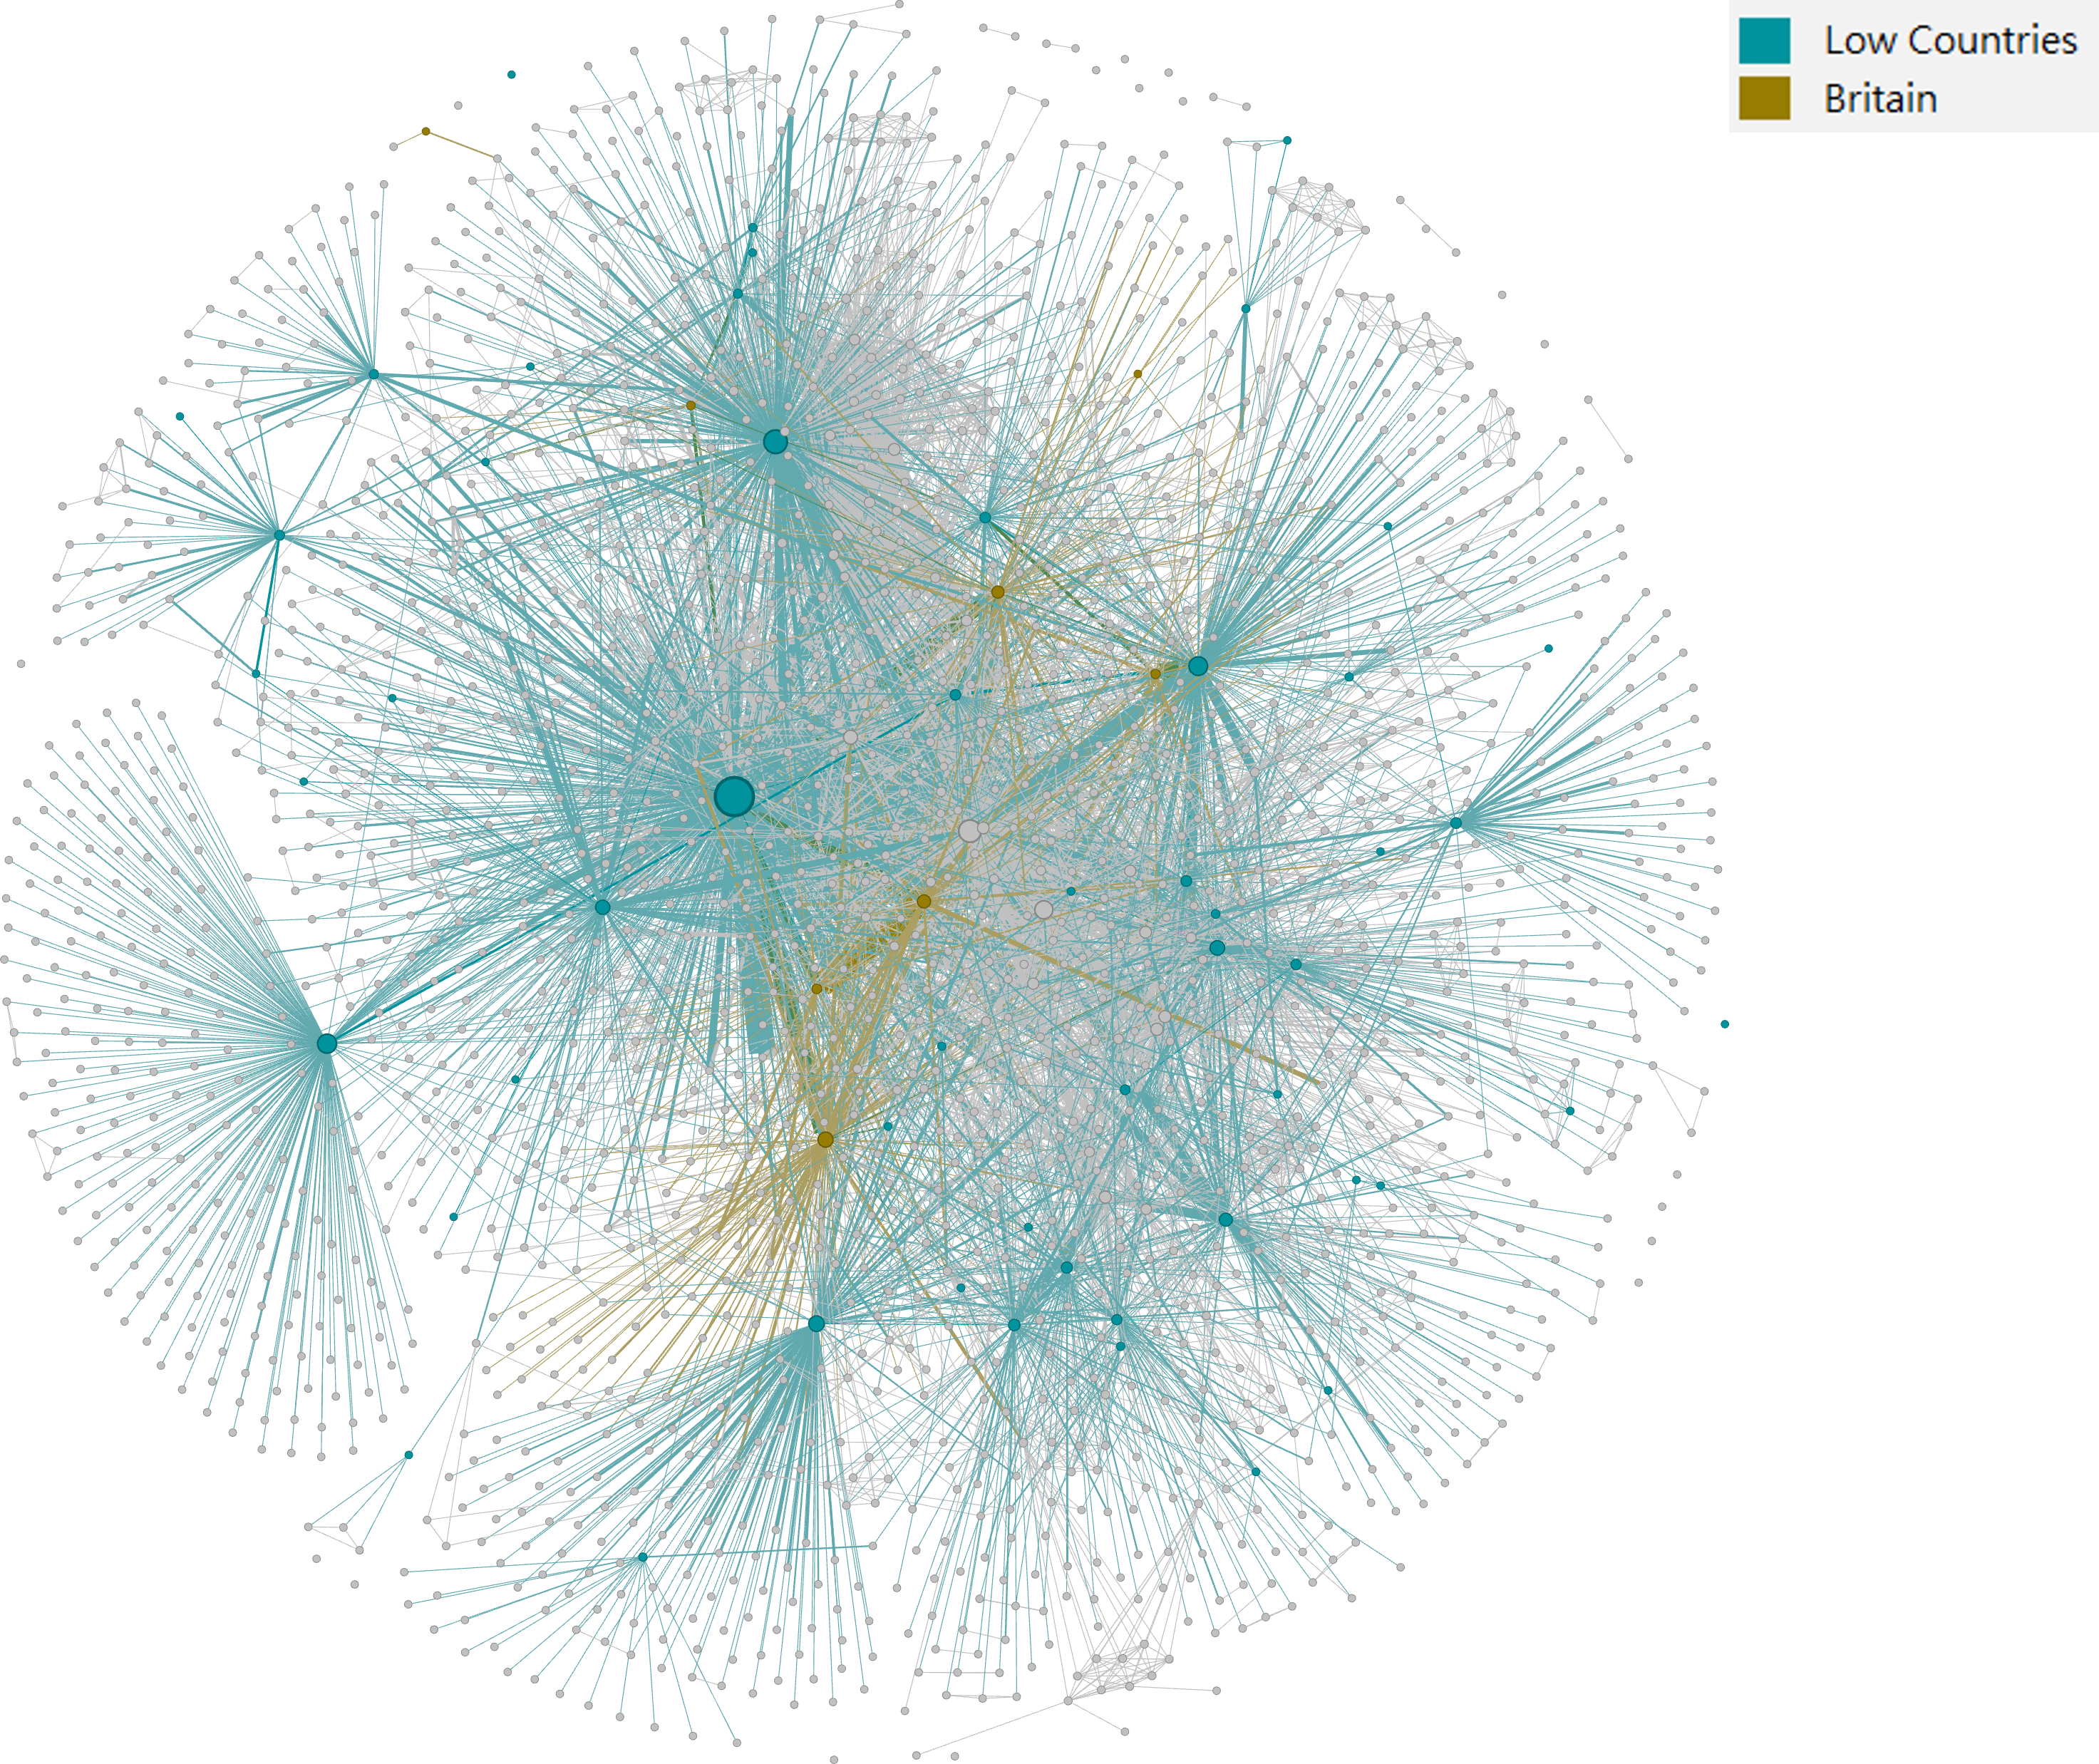
\includegraphics[scale=0.5]{graph/People Network Only Nodes Belonging to a Printing House were Coloured.png}
\caption{People Network Only Nodes Belonging to a Printing House were Coloured}
\label{fig:onlyPrint}
\end{figure}

If we keep only these houses in the Network (Figure \ref{fig:printHouse}), we can get a sharp vision that the printing houses of Bellère and Kellam were connected stronger than any other two printing houses, aligning with the observation from the historians (Soetaert \& Wyffels, 2021) that these two families had an extensive collaboration in the Douai publishing industry. We can also conduct Modularity to determine their collaboration. Modularity measures how well a Network can be divided into subgroups (Carrington \& Scott, 2011; Wasserman \& Faust, 1994), and it would give each divided group a Modularity Class. From Table \ref{tab:modularityClass} you can see 4 out of 8 members of these two houses are categorised in the same class. Furthermore, it seems that the house of Kellam was more connected to Balthazar I Bellère himself instead of the whole Bellère house since Balthazar I Bellère is the only one in the same class as the members of Kellam.

\begin{figure}[H]
\centering
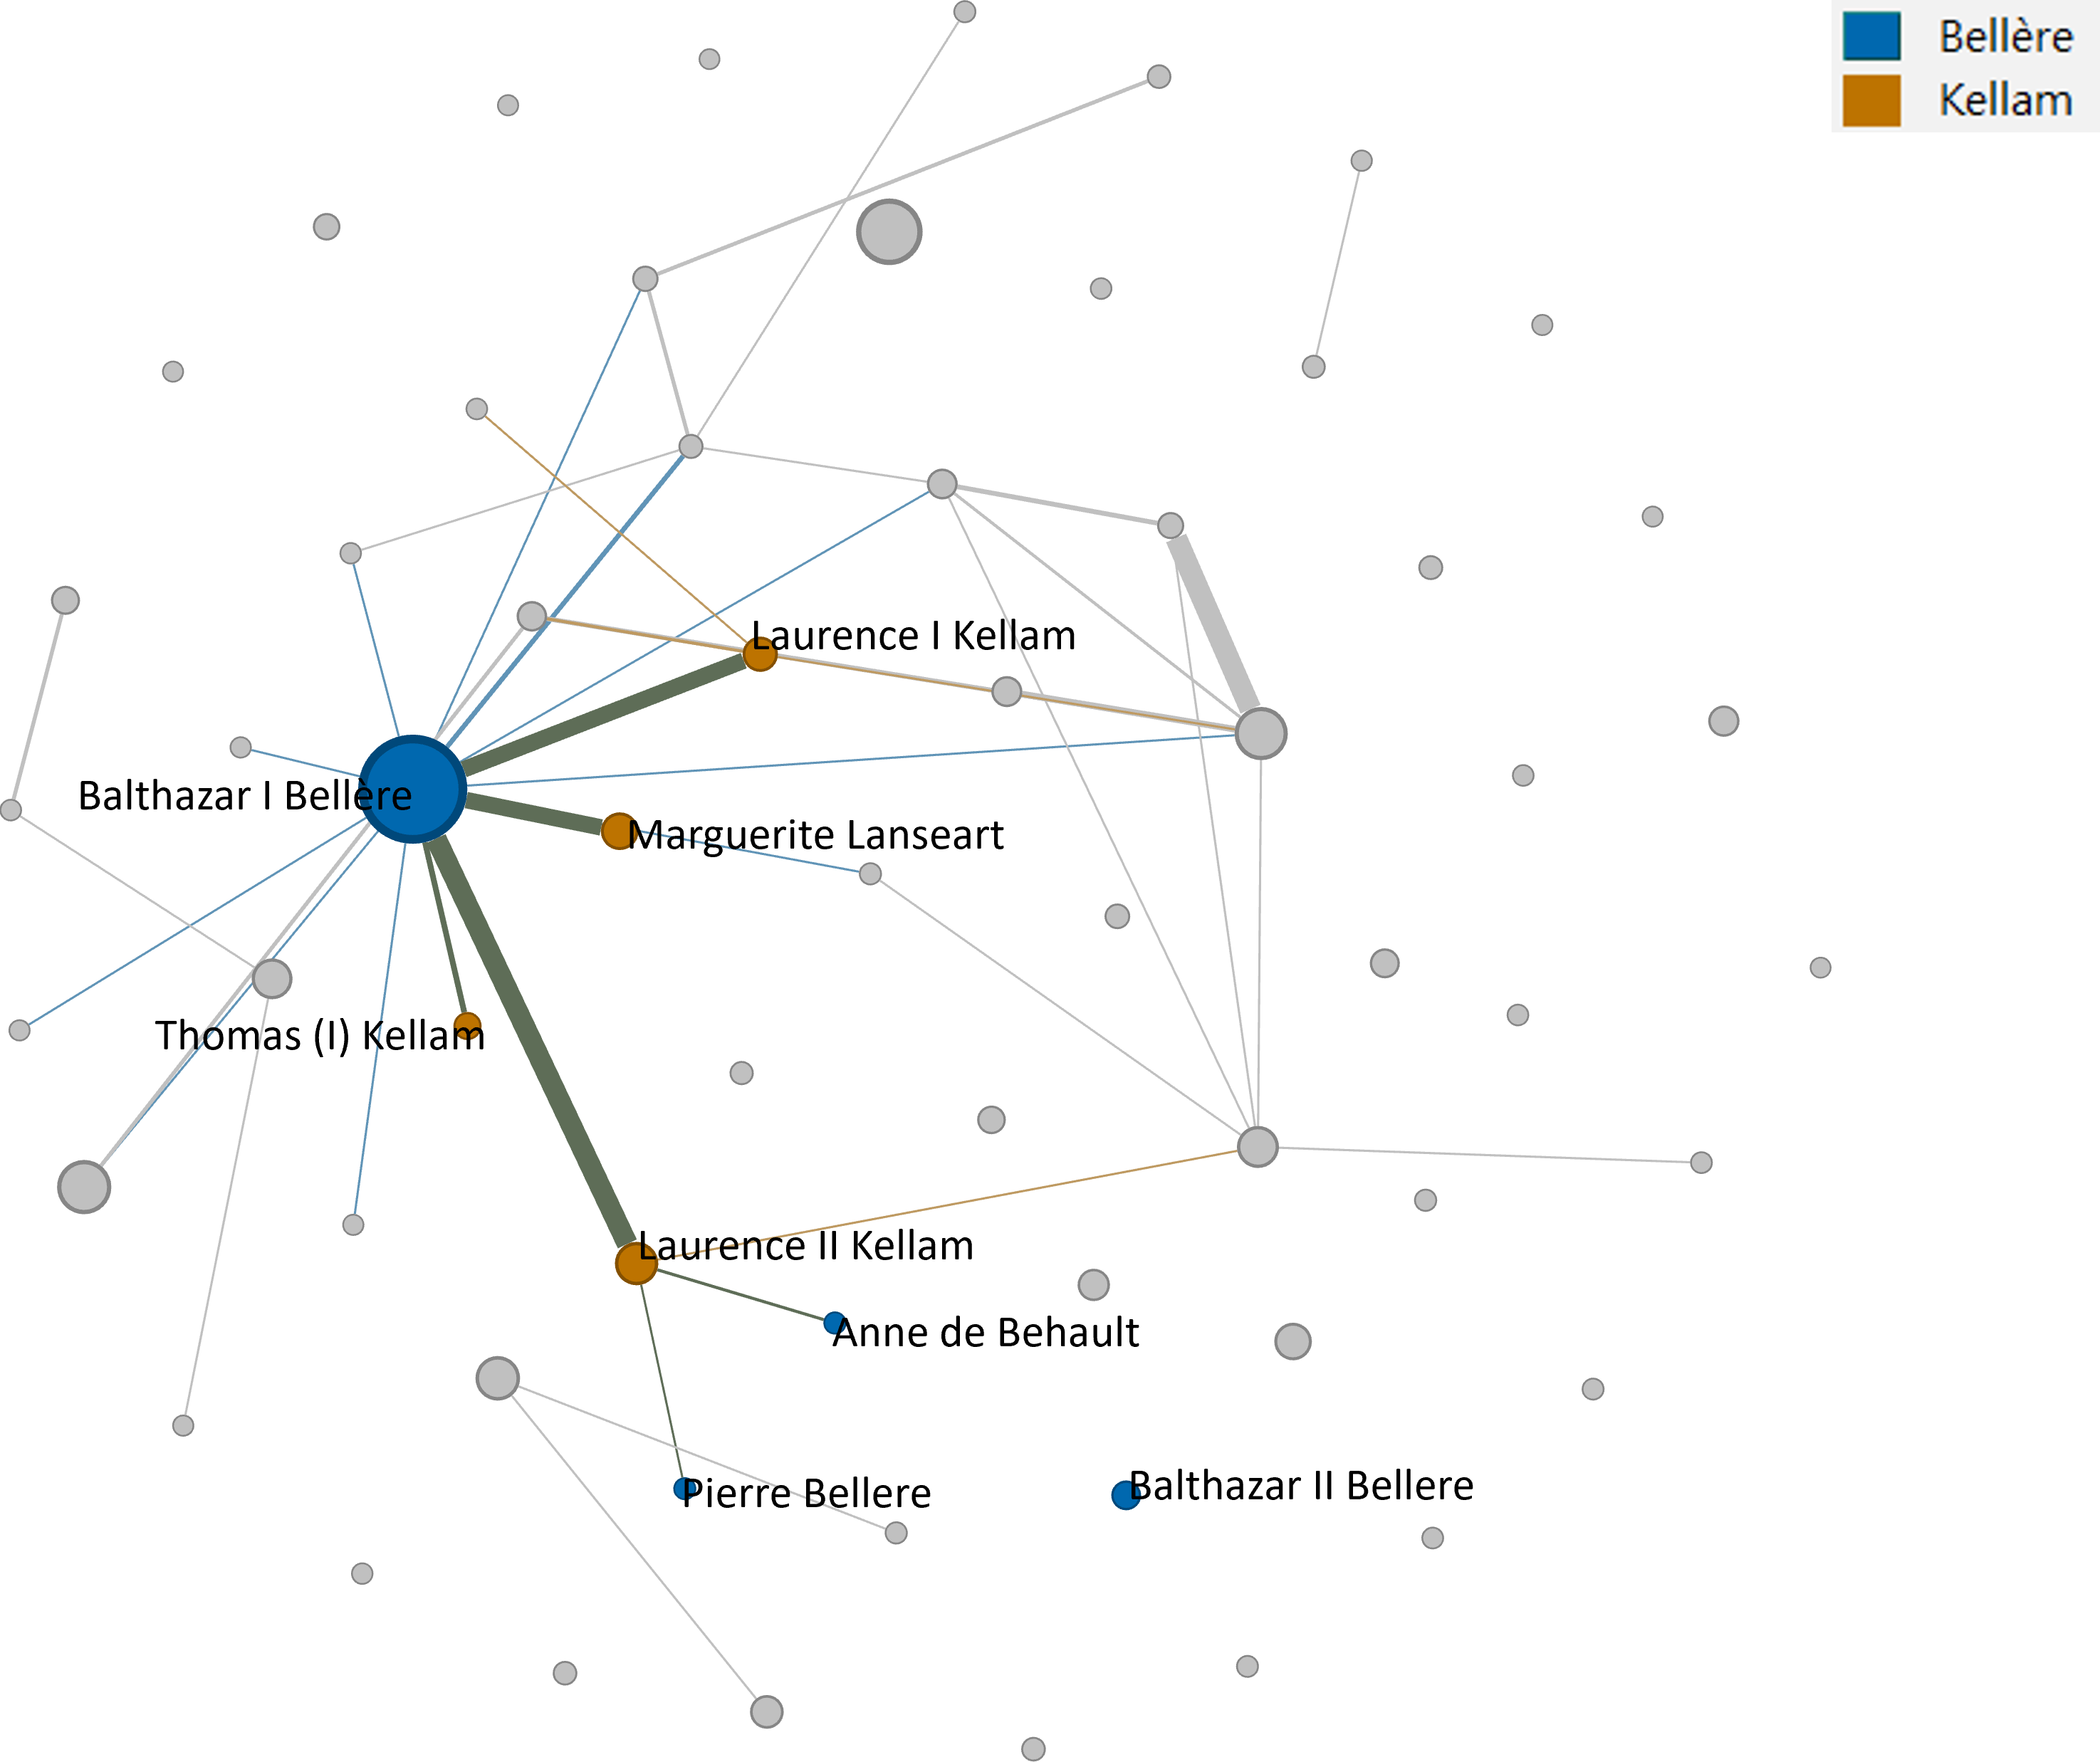
\includegraphics[scale=0.55]{graph/Network of Only Printing Houses.png}
\caption{Network of Only Printing Houses}
\label{fig:printHouse}
\end{figure}

\begin{table}[H]
\centering
\caption{Modularity Class of the Two Printing Houses}
\label{tab:modularityClass}
\resizebox{\textwidth}{!}{
\begin{tabular}{lclc}
\multicolumn{2}{c|}{\textbf{Bellère}}                                                       & \multicolumn{2}{c}{\textbf{Kellam}}                                                       \\ \hline
\multicolumn{1}{c}{\textbf{Name}}          & \multicolumn{1}{c|}{\textbf{Modularity Class}} & \multicolumn{1}{c}{\textbf{Name}}         & {\textbf{Modularity Class}} \\ \hline
{\color[HTML]{303498} Balthazar I Bellère} & \multicolumn{1}{c|}{{\color[HTML]{303498} 13}} & {\color[HTML]{303498} Laurence I Kellam}  & {\color[HTML]{303498} 13}                     \\
Anne de Behault                            & \multicolumn{1}{c|}{8}                         & Marguerite Lanseart                       & 12                                            \\
Pierre Bellere                             & \multicolumn{1}{c|}{9}                         & {\color[HTML]{303498} Laurence II Kellam} & {\color[HTML]{303498} 13}                     \\
Balthazar II Bellere                       & \multicolumn{1}{c|}{10}                        & {\color[HTML]{303498} Thomas (I) Kellam}  & {\color[HTML]{303498} 13}                     \\ \hline
\multicolumn{4}{l}{* {\color[HTML]{303498} Blue} means they are in the same Modularity Class\tablefootnote{By numbering the outcome of community detection from NetworkX, with the resolution of 1.0.}}                                                                                                                 
\end{tabular}
}
\end{table}

In addition, we can also graph a clearer establishment between the two printing houses by the Network (Figure \ref{fig:interactionBelAndKel}). You can see their collaboration started in the 1600s with the connection of both founders (Wyffels, 2017m, 2018f), Balthazar I Bellère and Laurence I Kellam. In the 1610s, since Laurence I Kellam died in 1612 (Soetaert et al., 2021), his wife, Marguerite Lanseart, was the one who represented the Kellam’s house to connect with the Bellère. Due to the death of Marguerite Lanseart in 1623 (Soetaert et al., 2023b), two houses stopped connecting during the 1620s. From the 1630s they reattached, surprisingly, by the connection between Laurence II Kellam, who took over the Kellam printing house after 1620 (Soetaert, 2020a), and Balthazar I Bellère’s wife and son (Soetaert et al., 2022a), Anne de Behault and Pierre Bellere. Heads of respective printing houses, Balthazar I Bellère and Laurence II Kellam, only connected briefly between 1642 and 1645, and then no connection is shown in this dataset.

\begin{figure}[H]
\centering
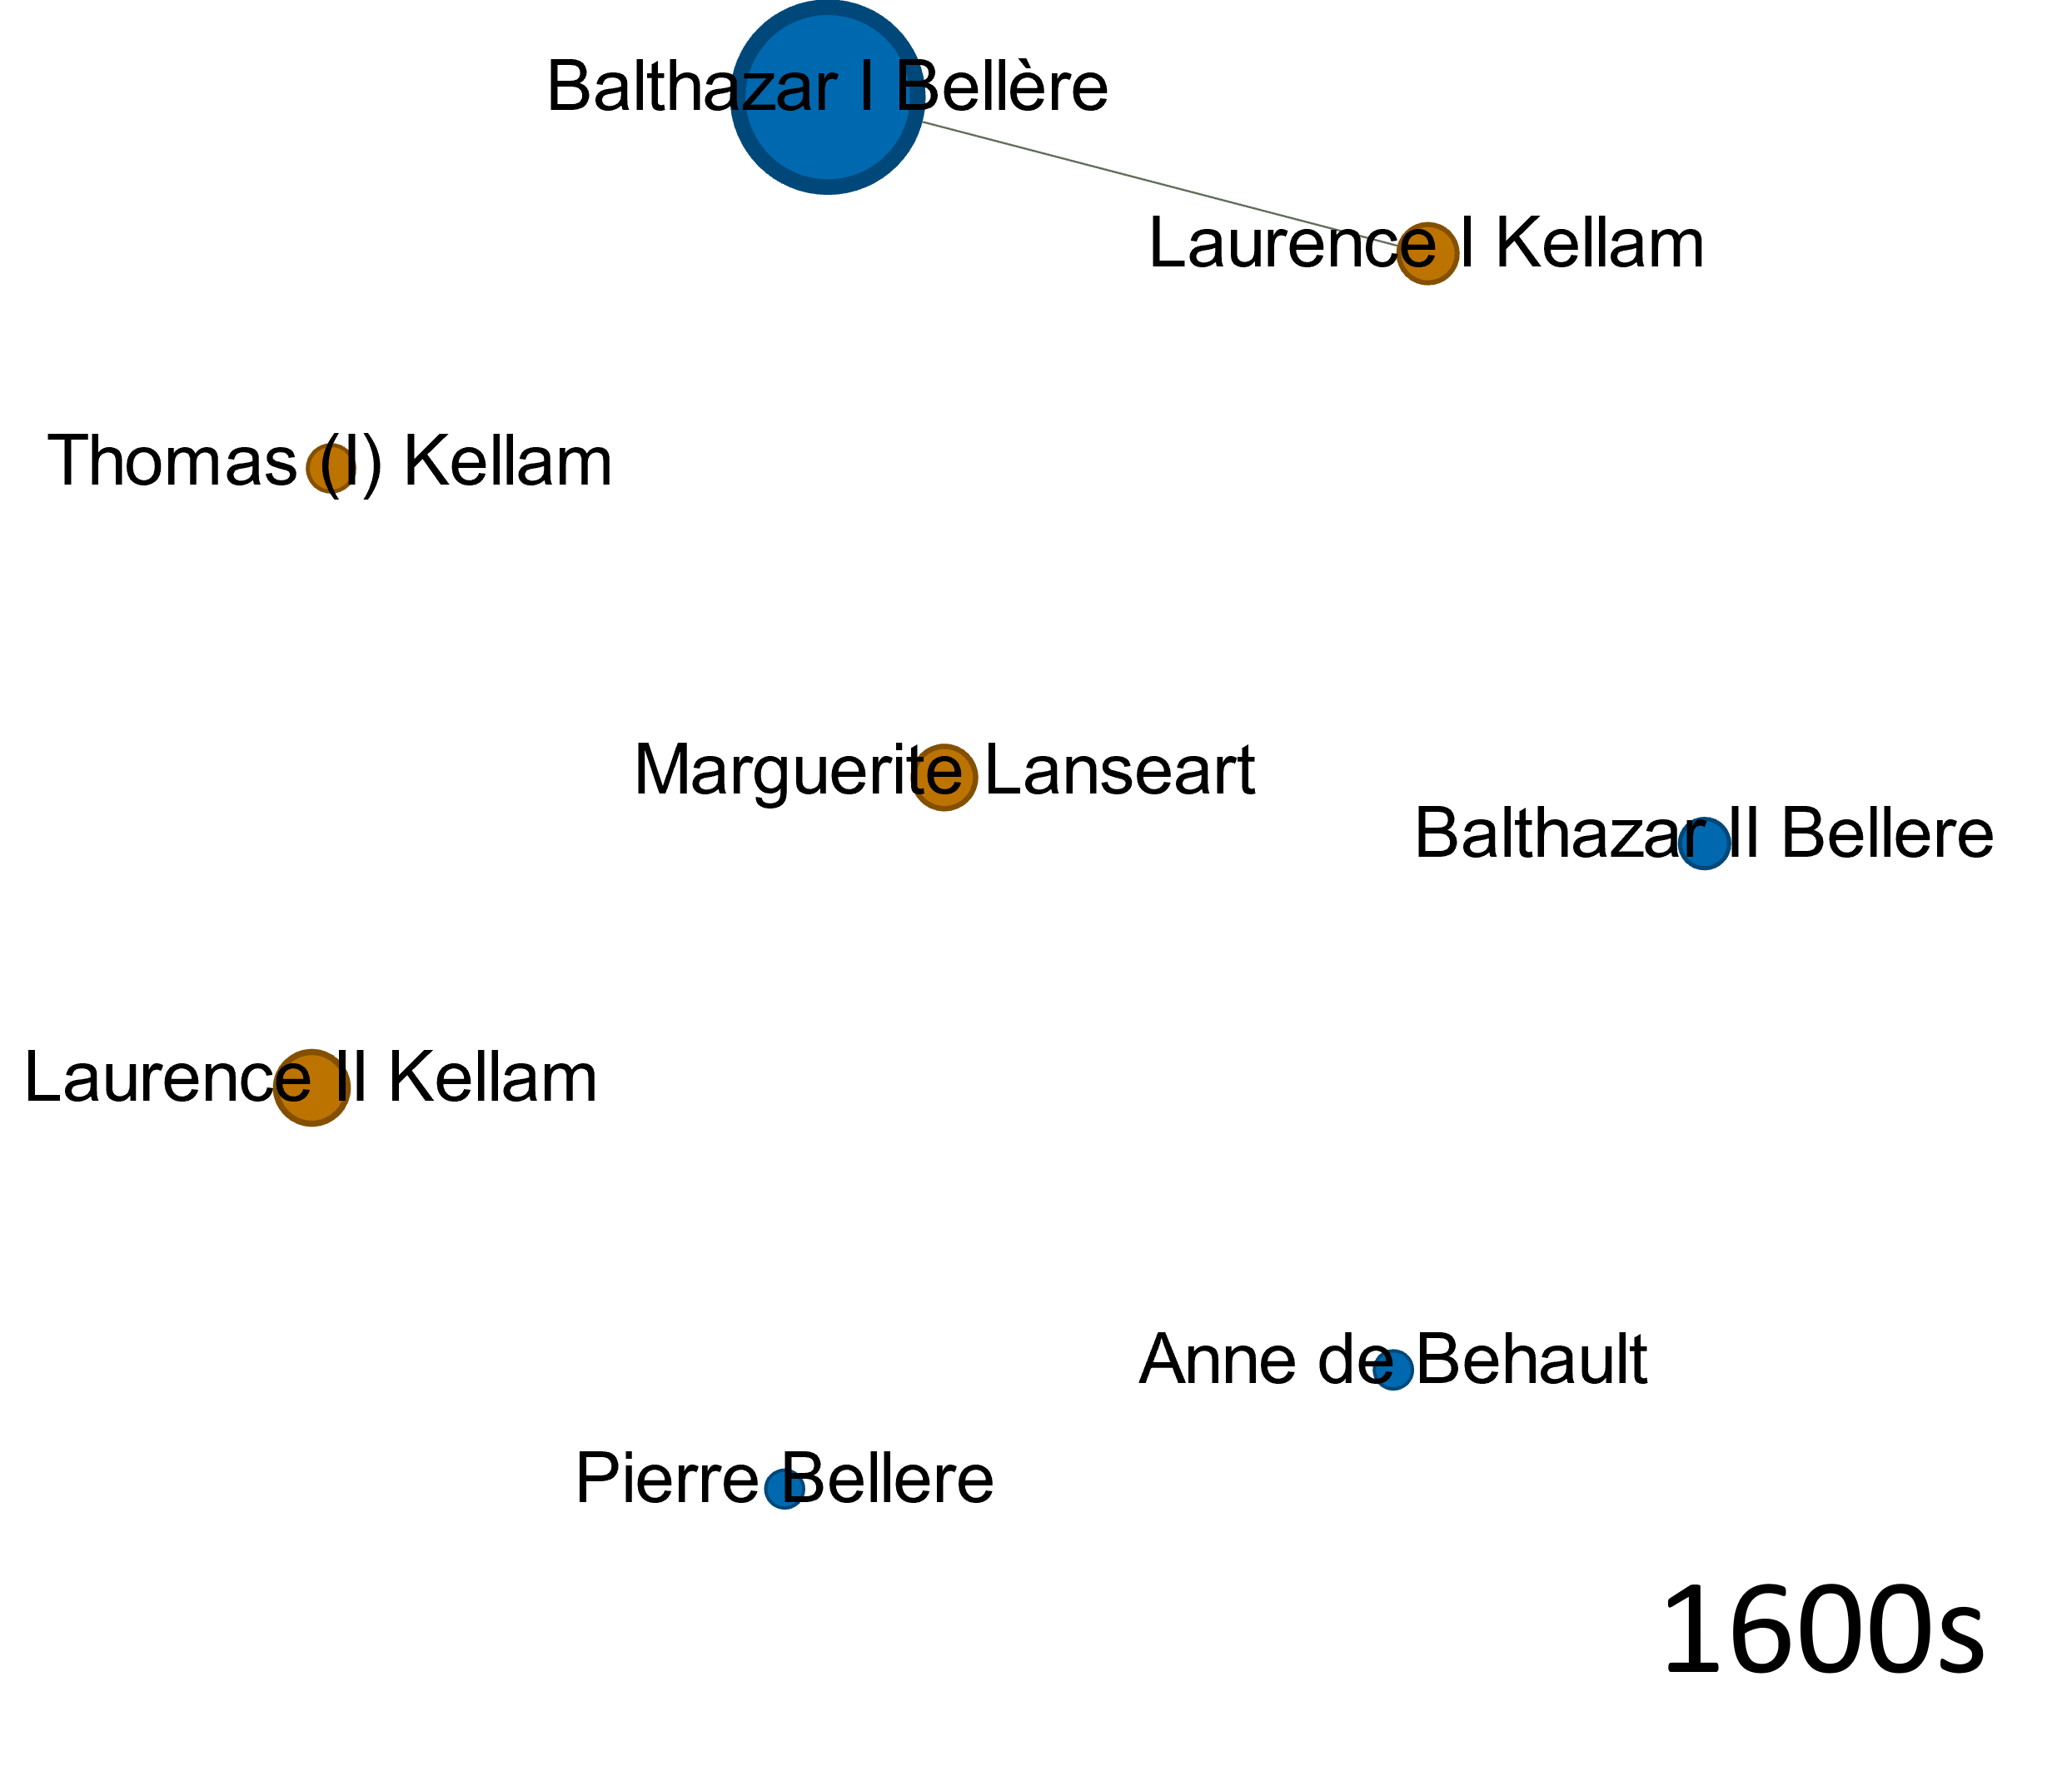
\includegraphics[scale=0.32]{graph/B&K_1600s.png}
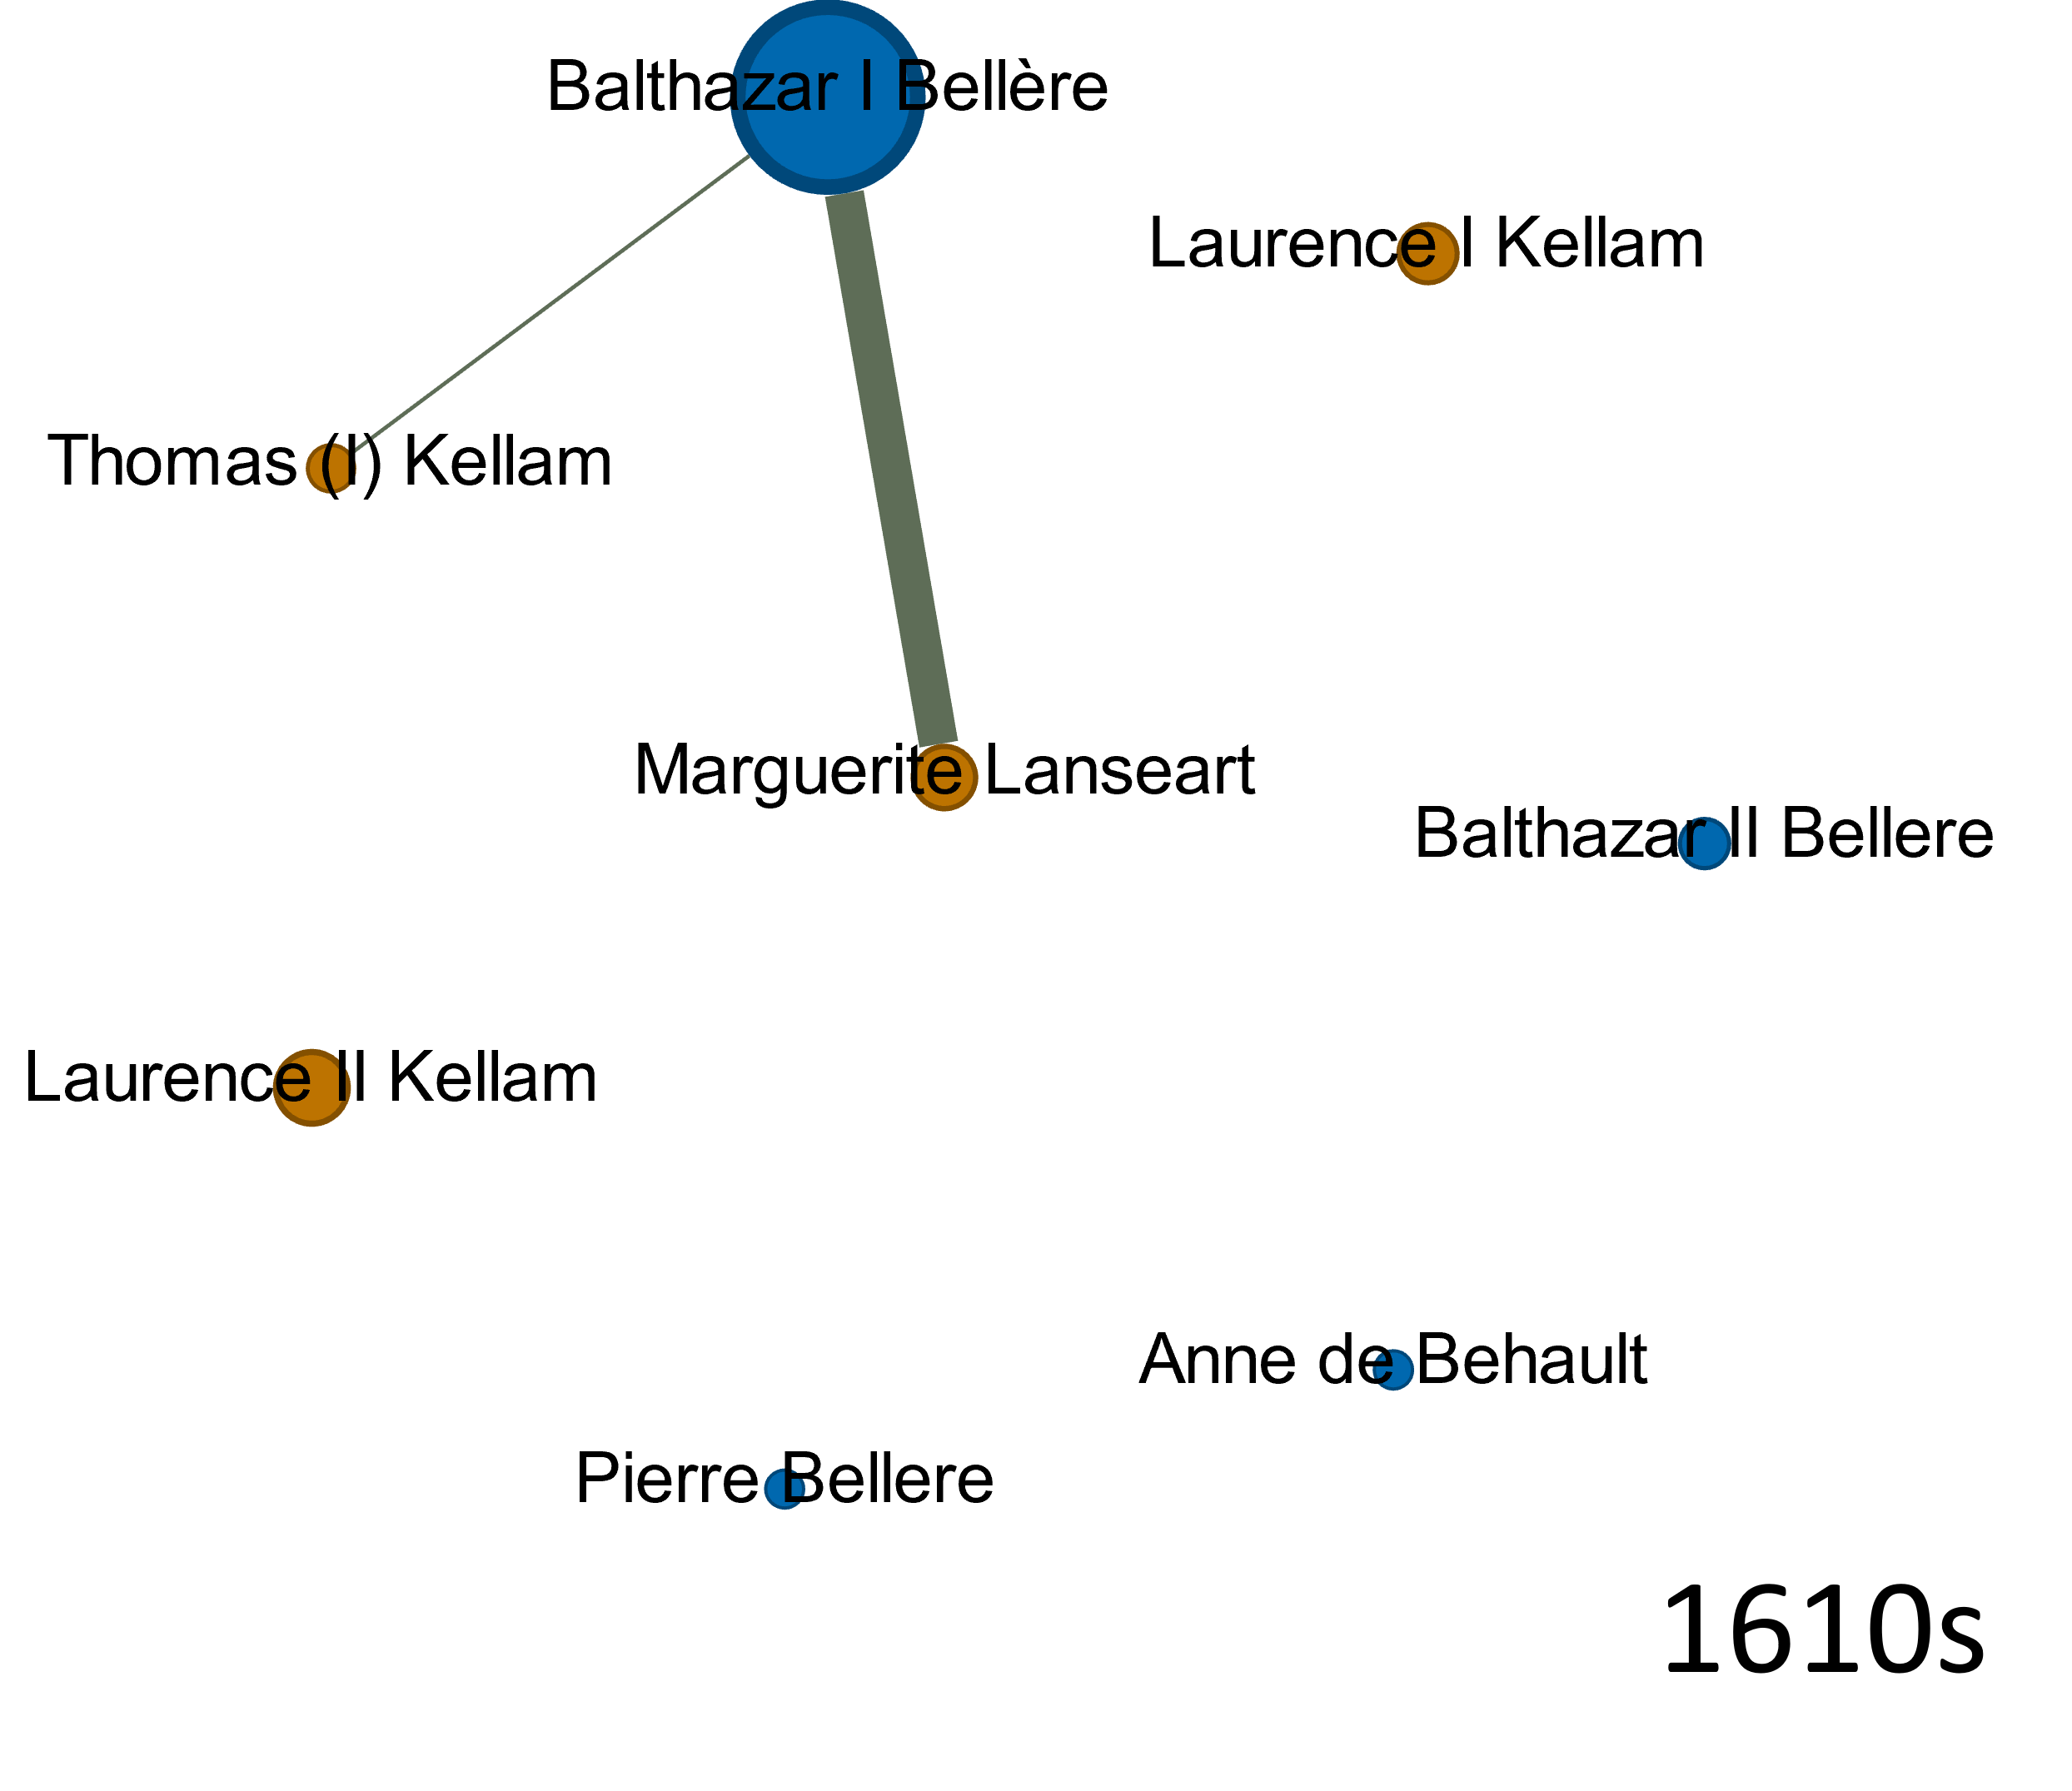
\includegraphics[scale=0.32]{graph/B&K_1610s.png}
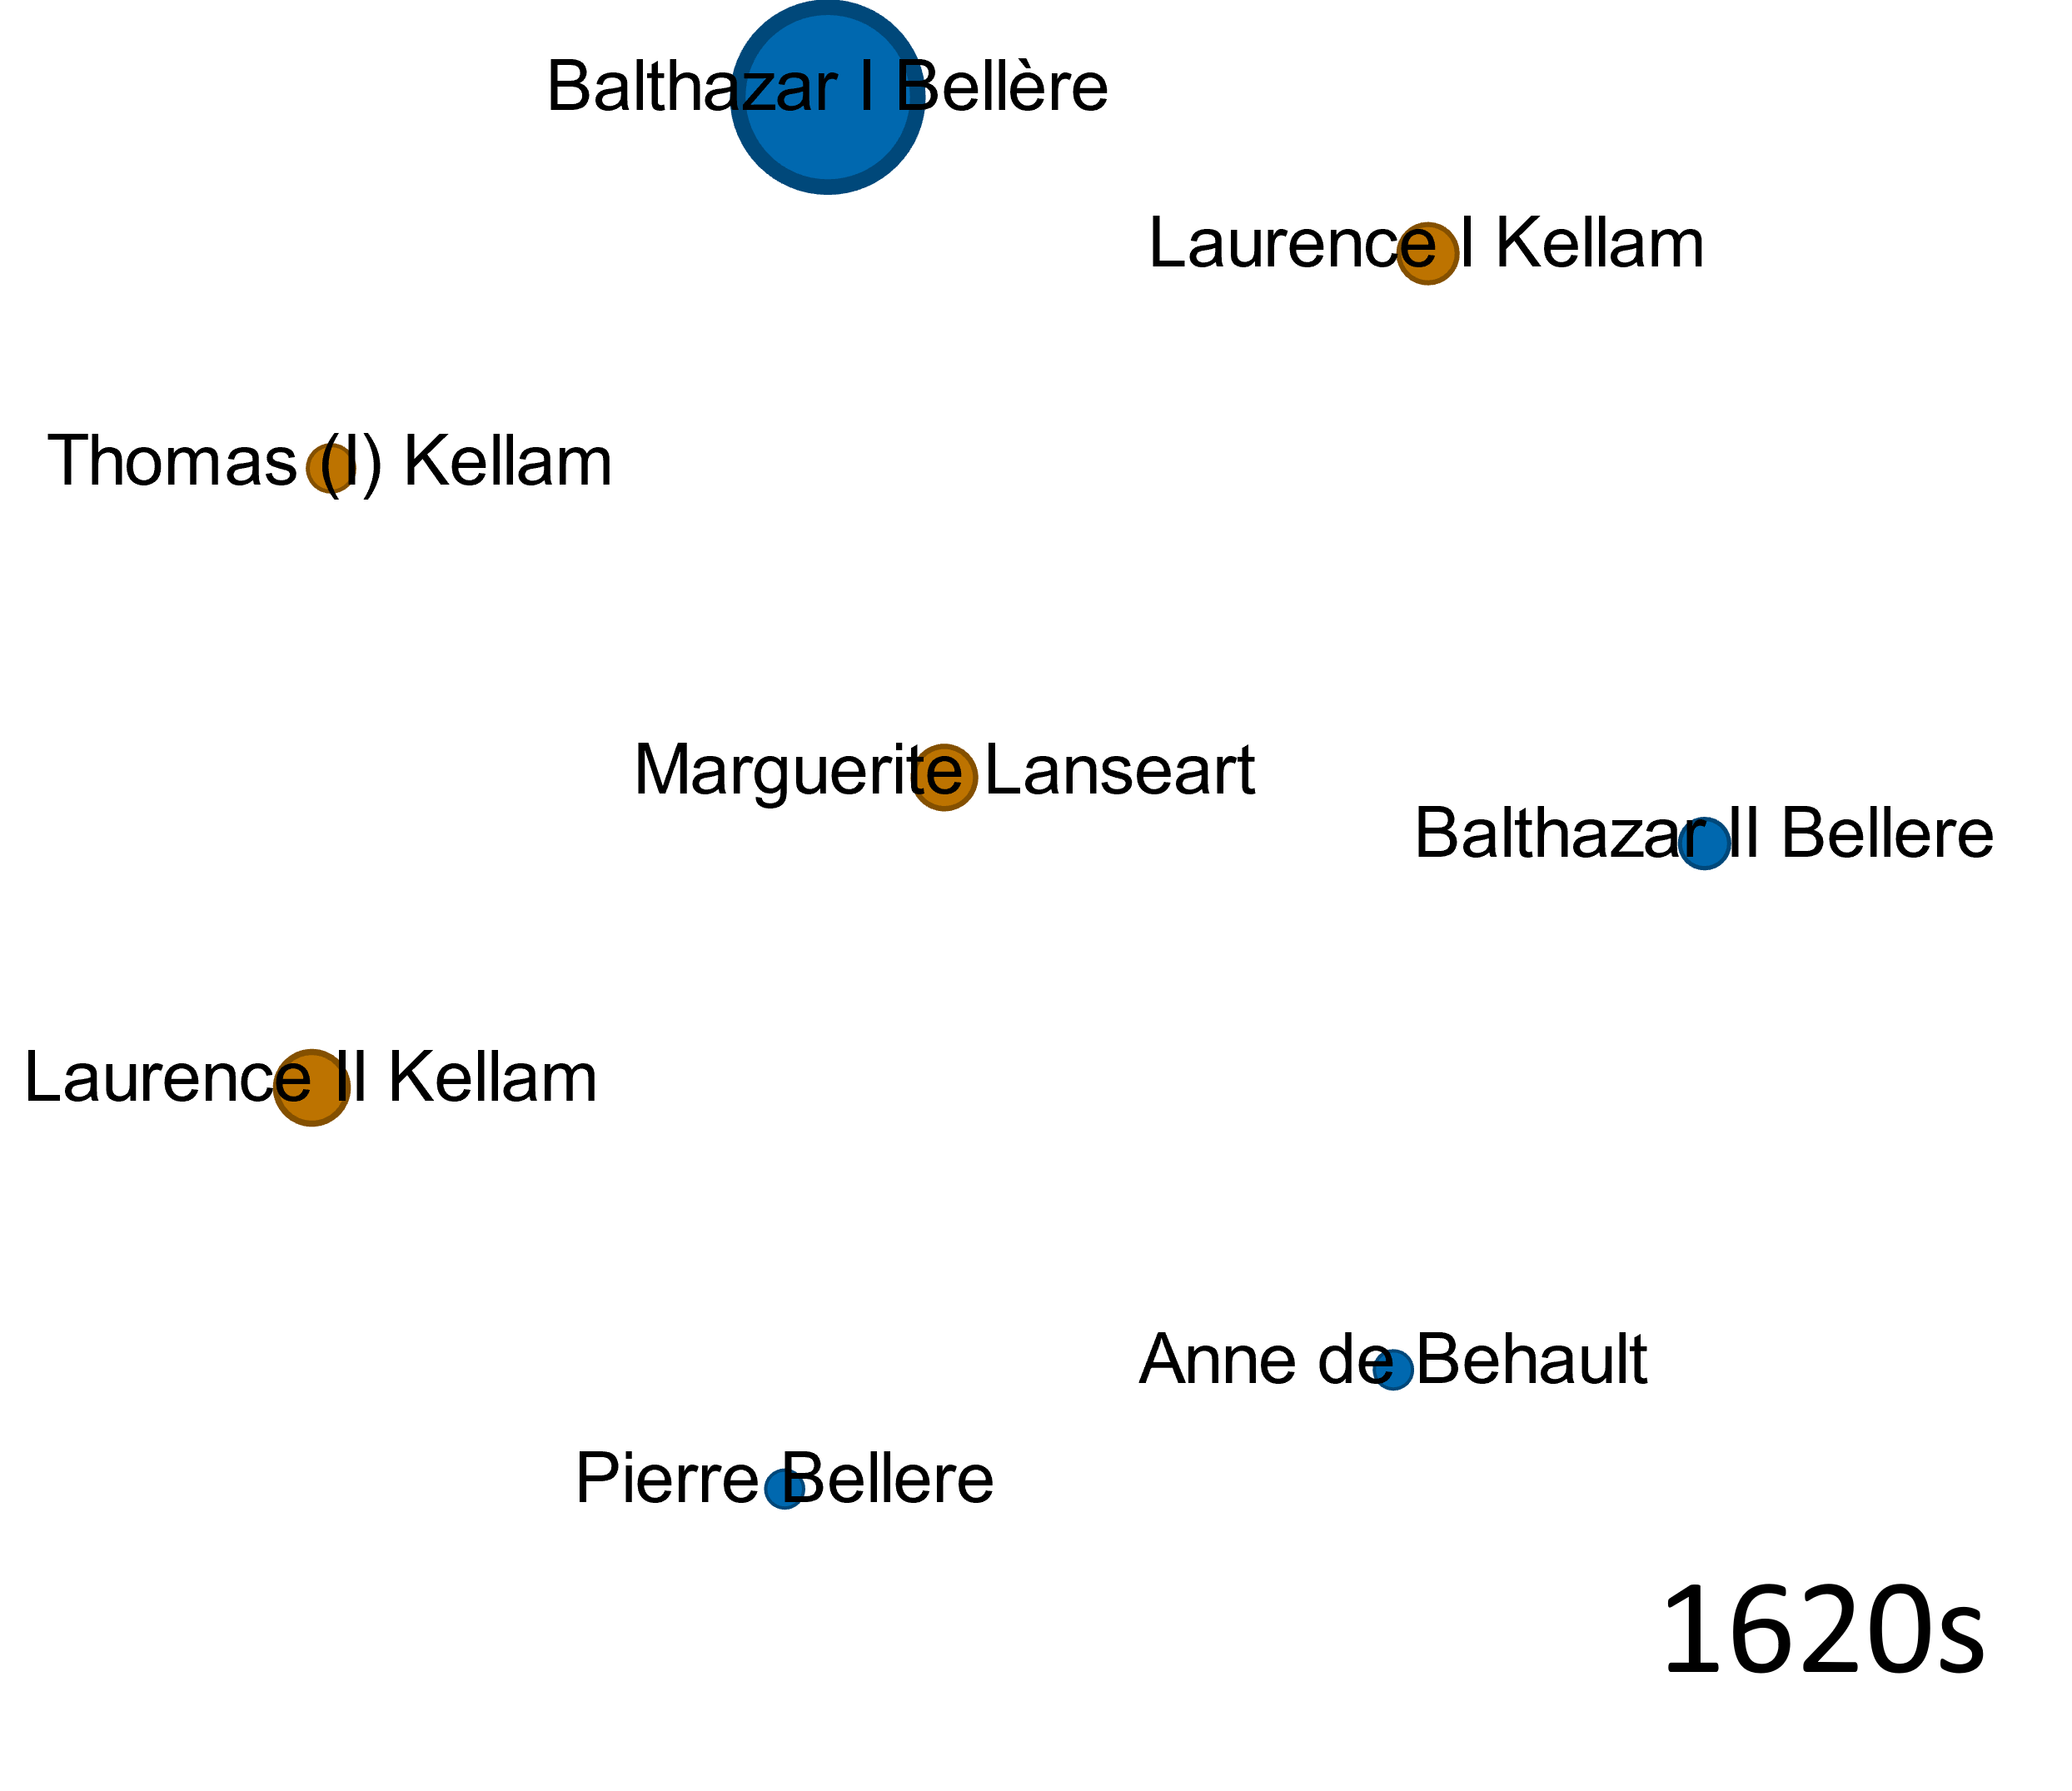
\includegraphics[scale=0.32]{graph/B&K_1620s.png}
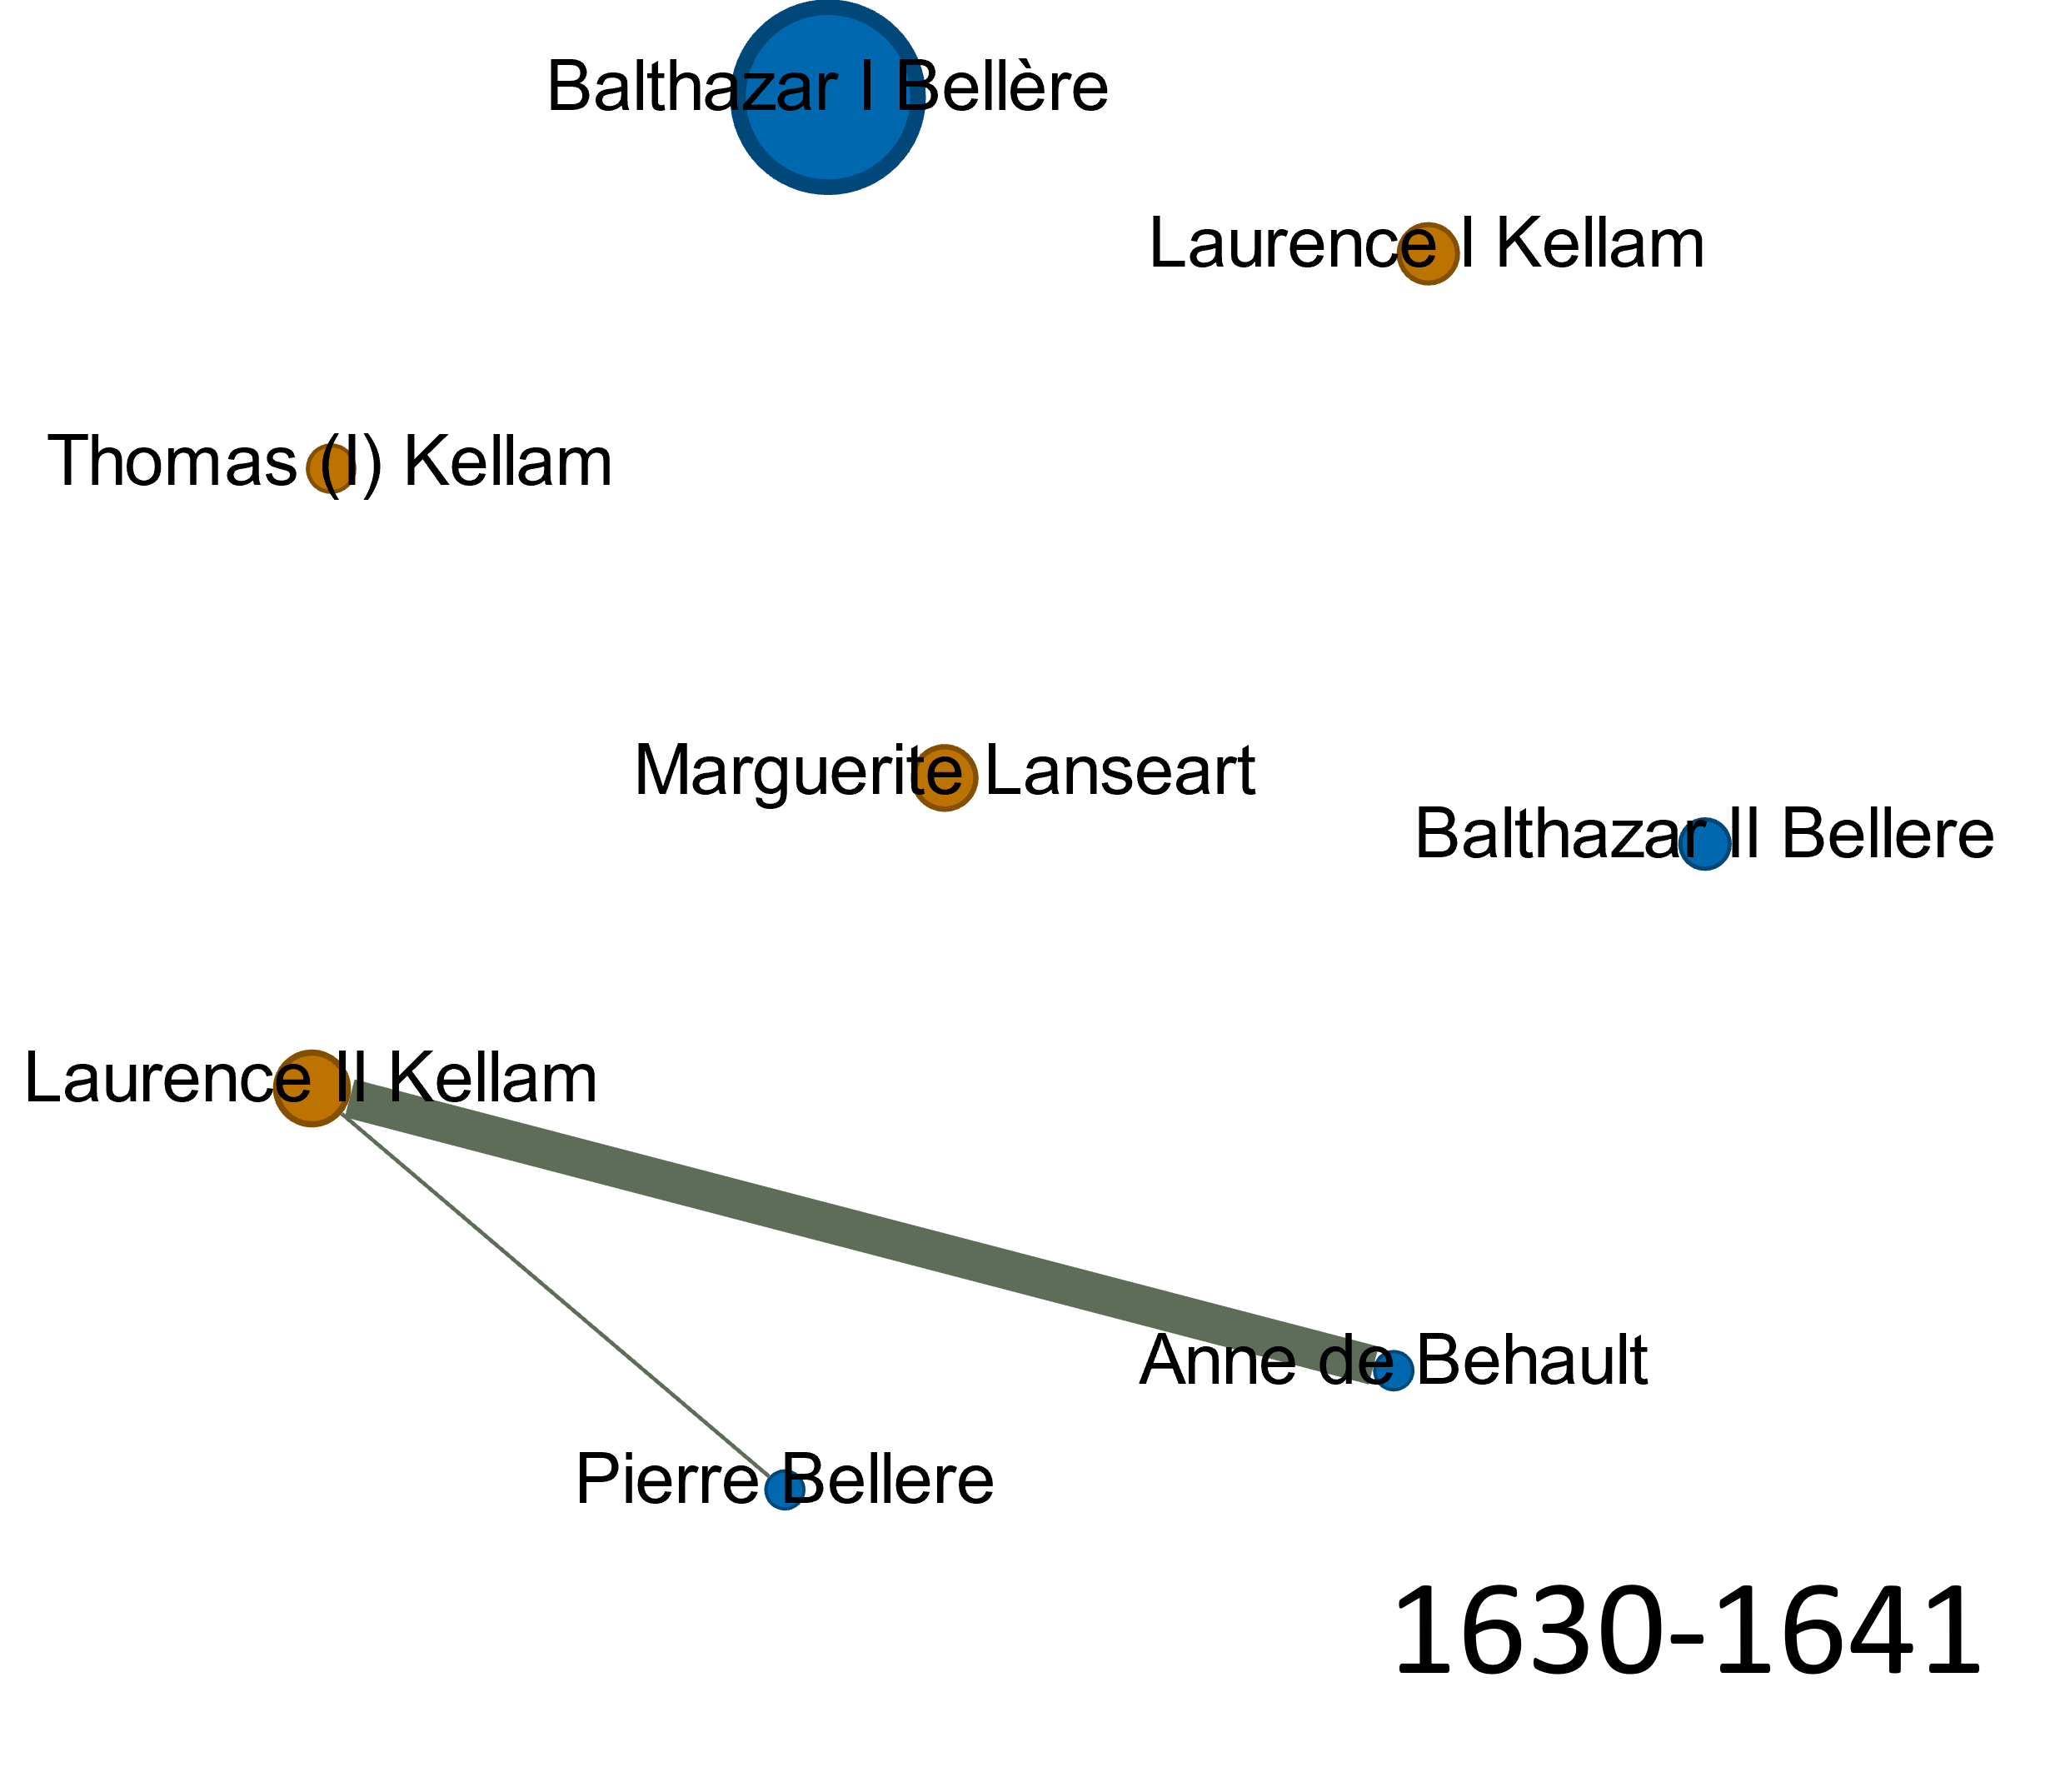
\includegraphics[scale=0.32]{graph/B&K_1630-1641.png}
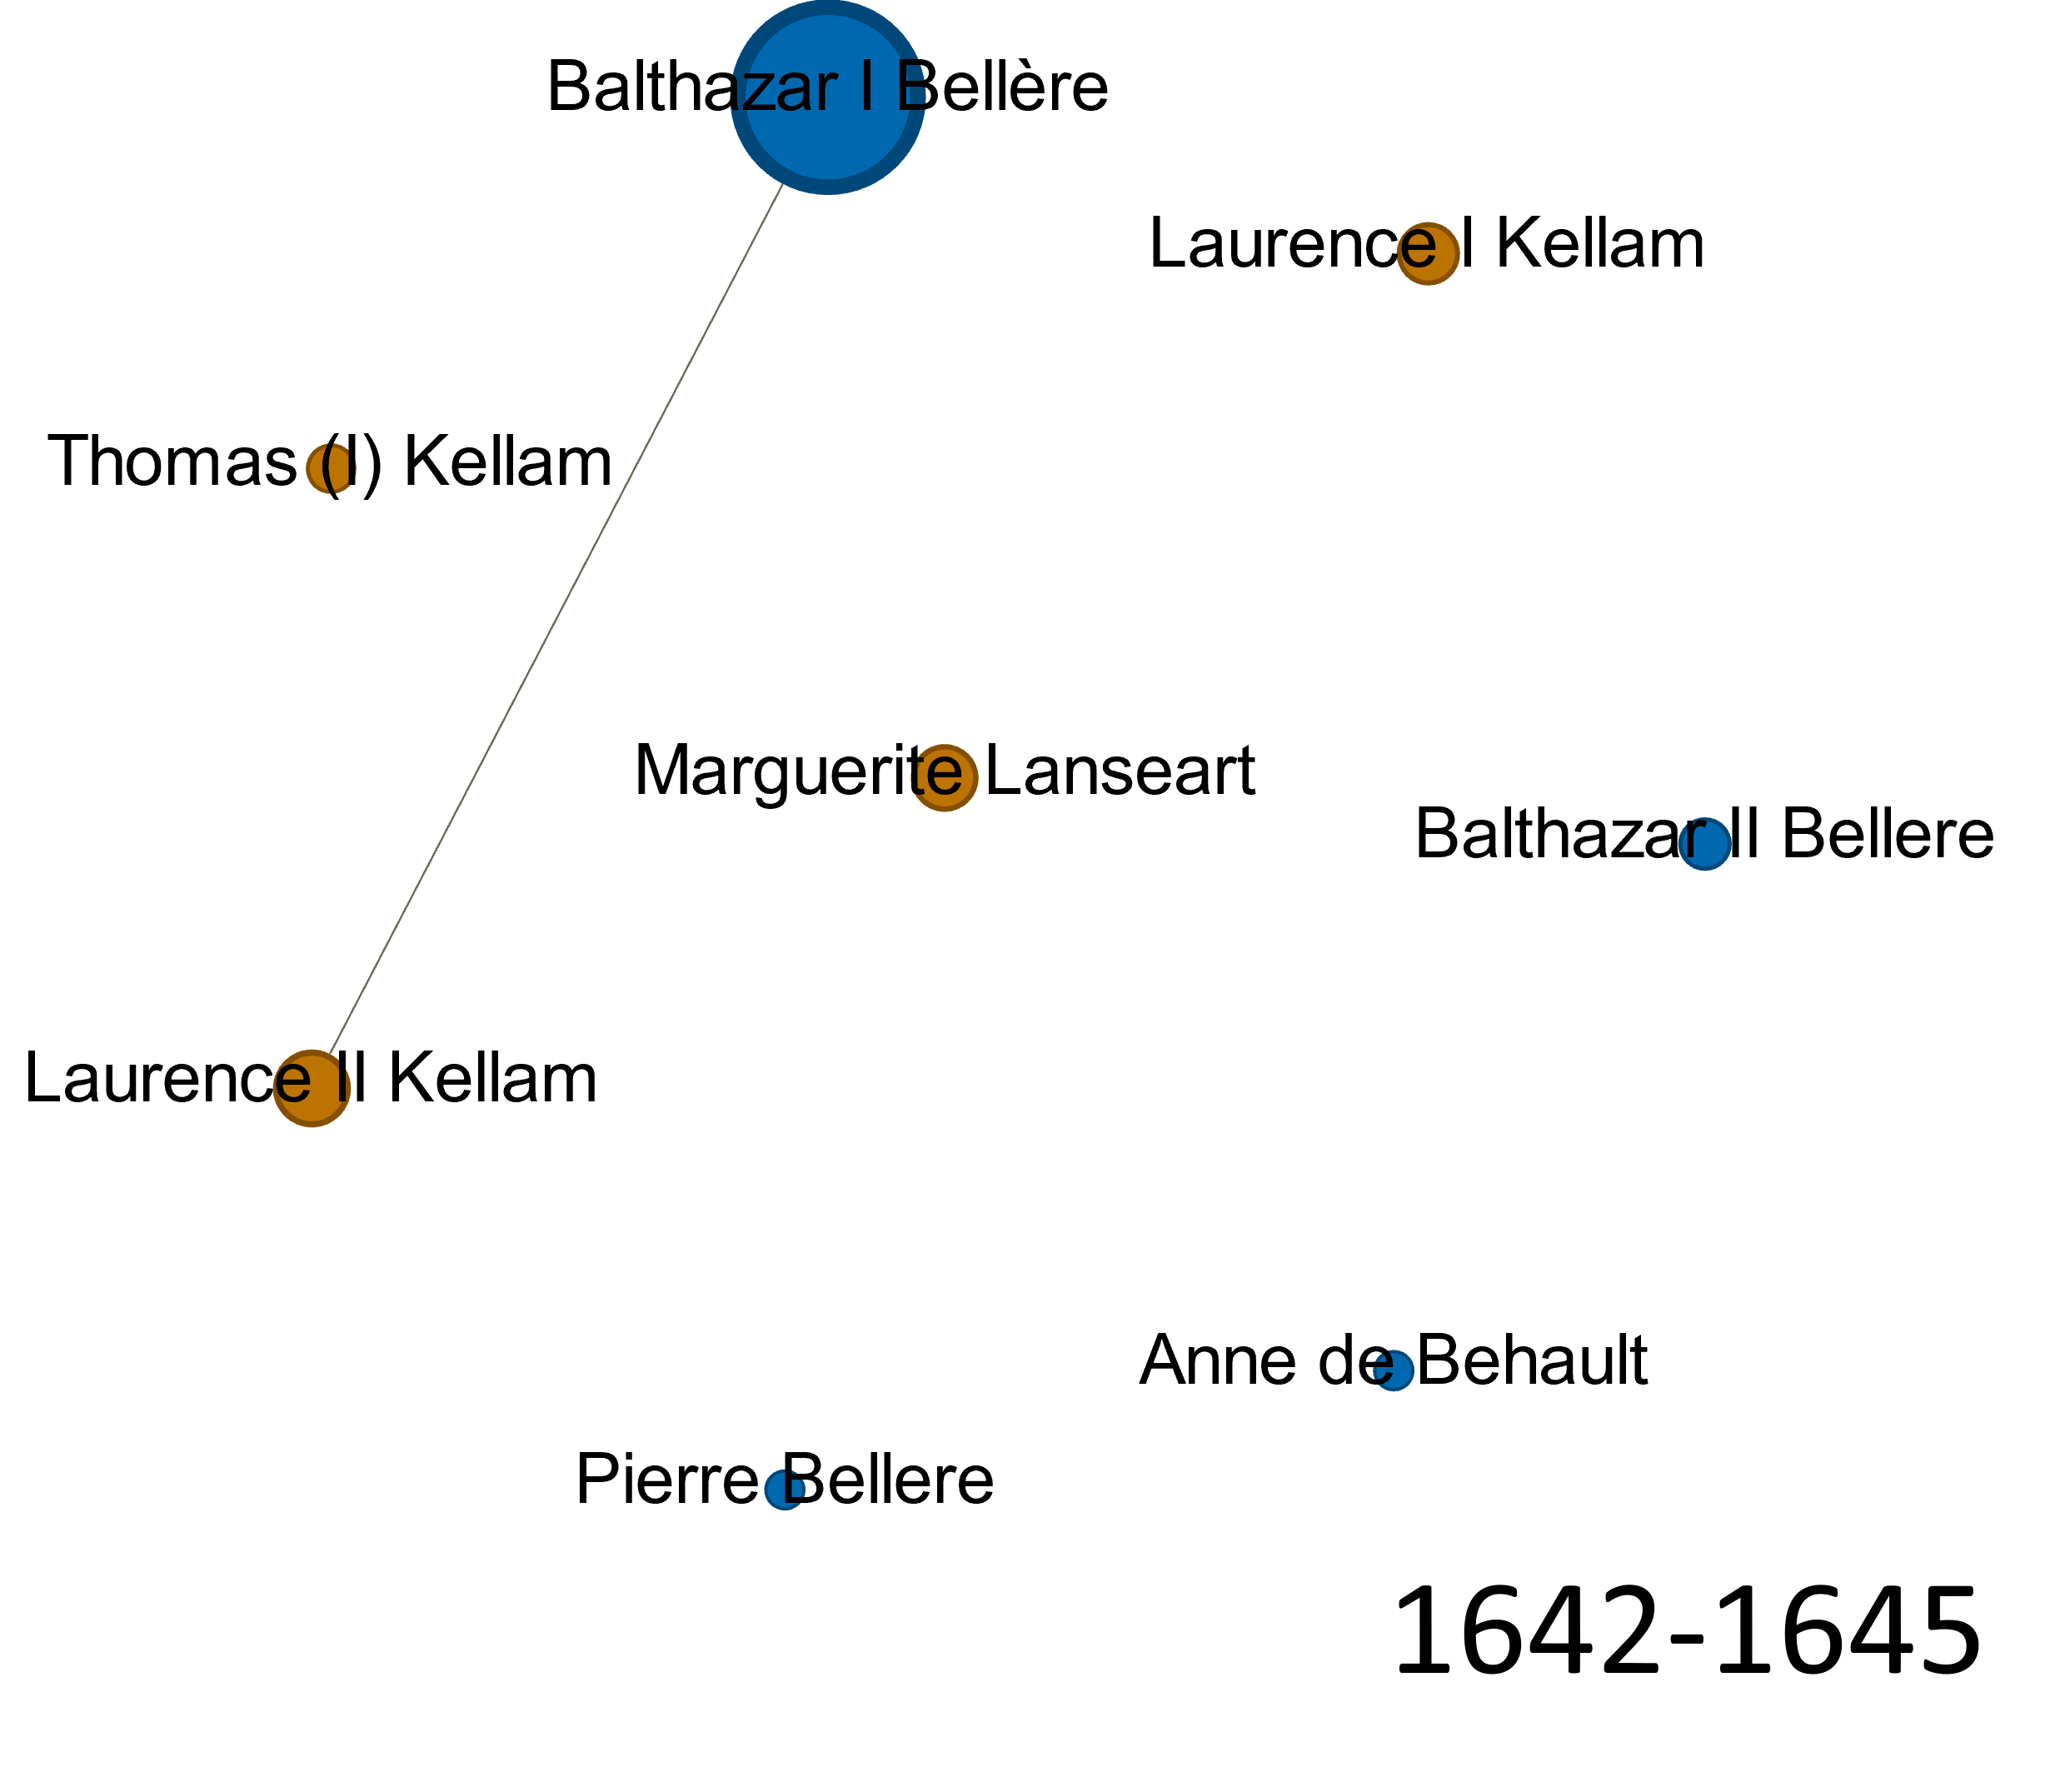
\includegraphics[scale=0.32]{graph/B&K_1642-1645.png}
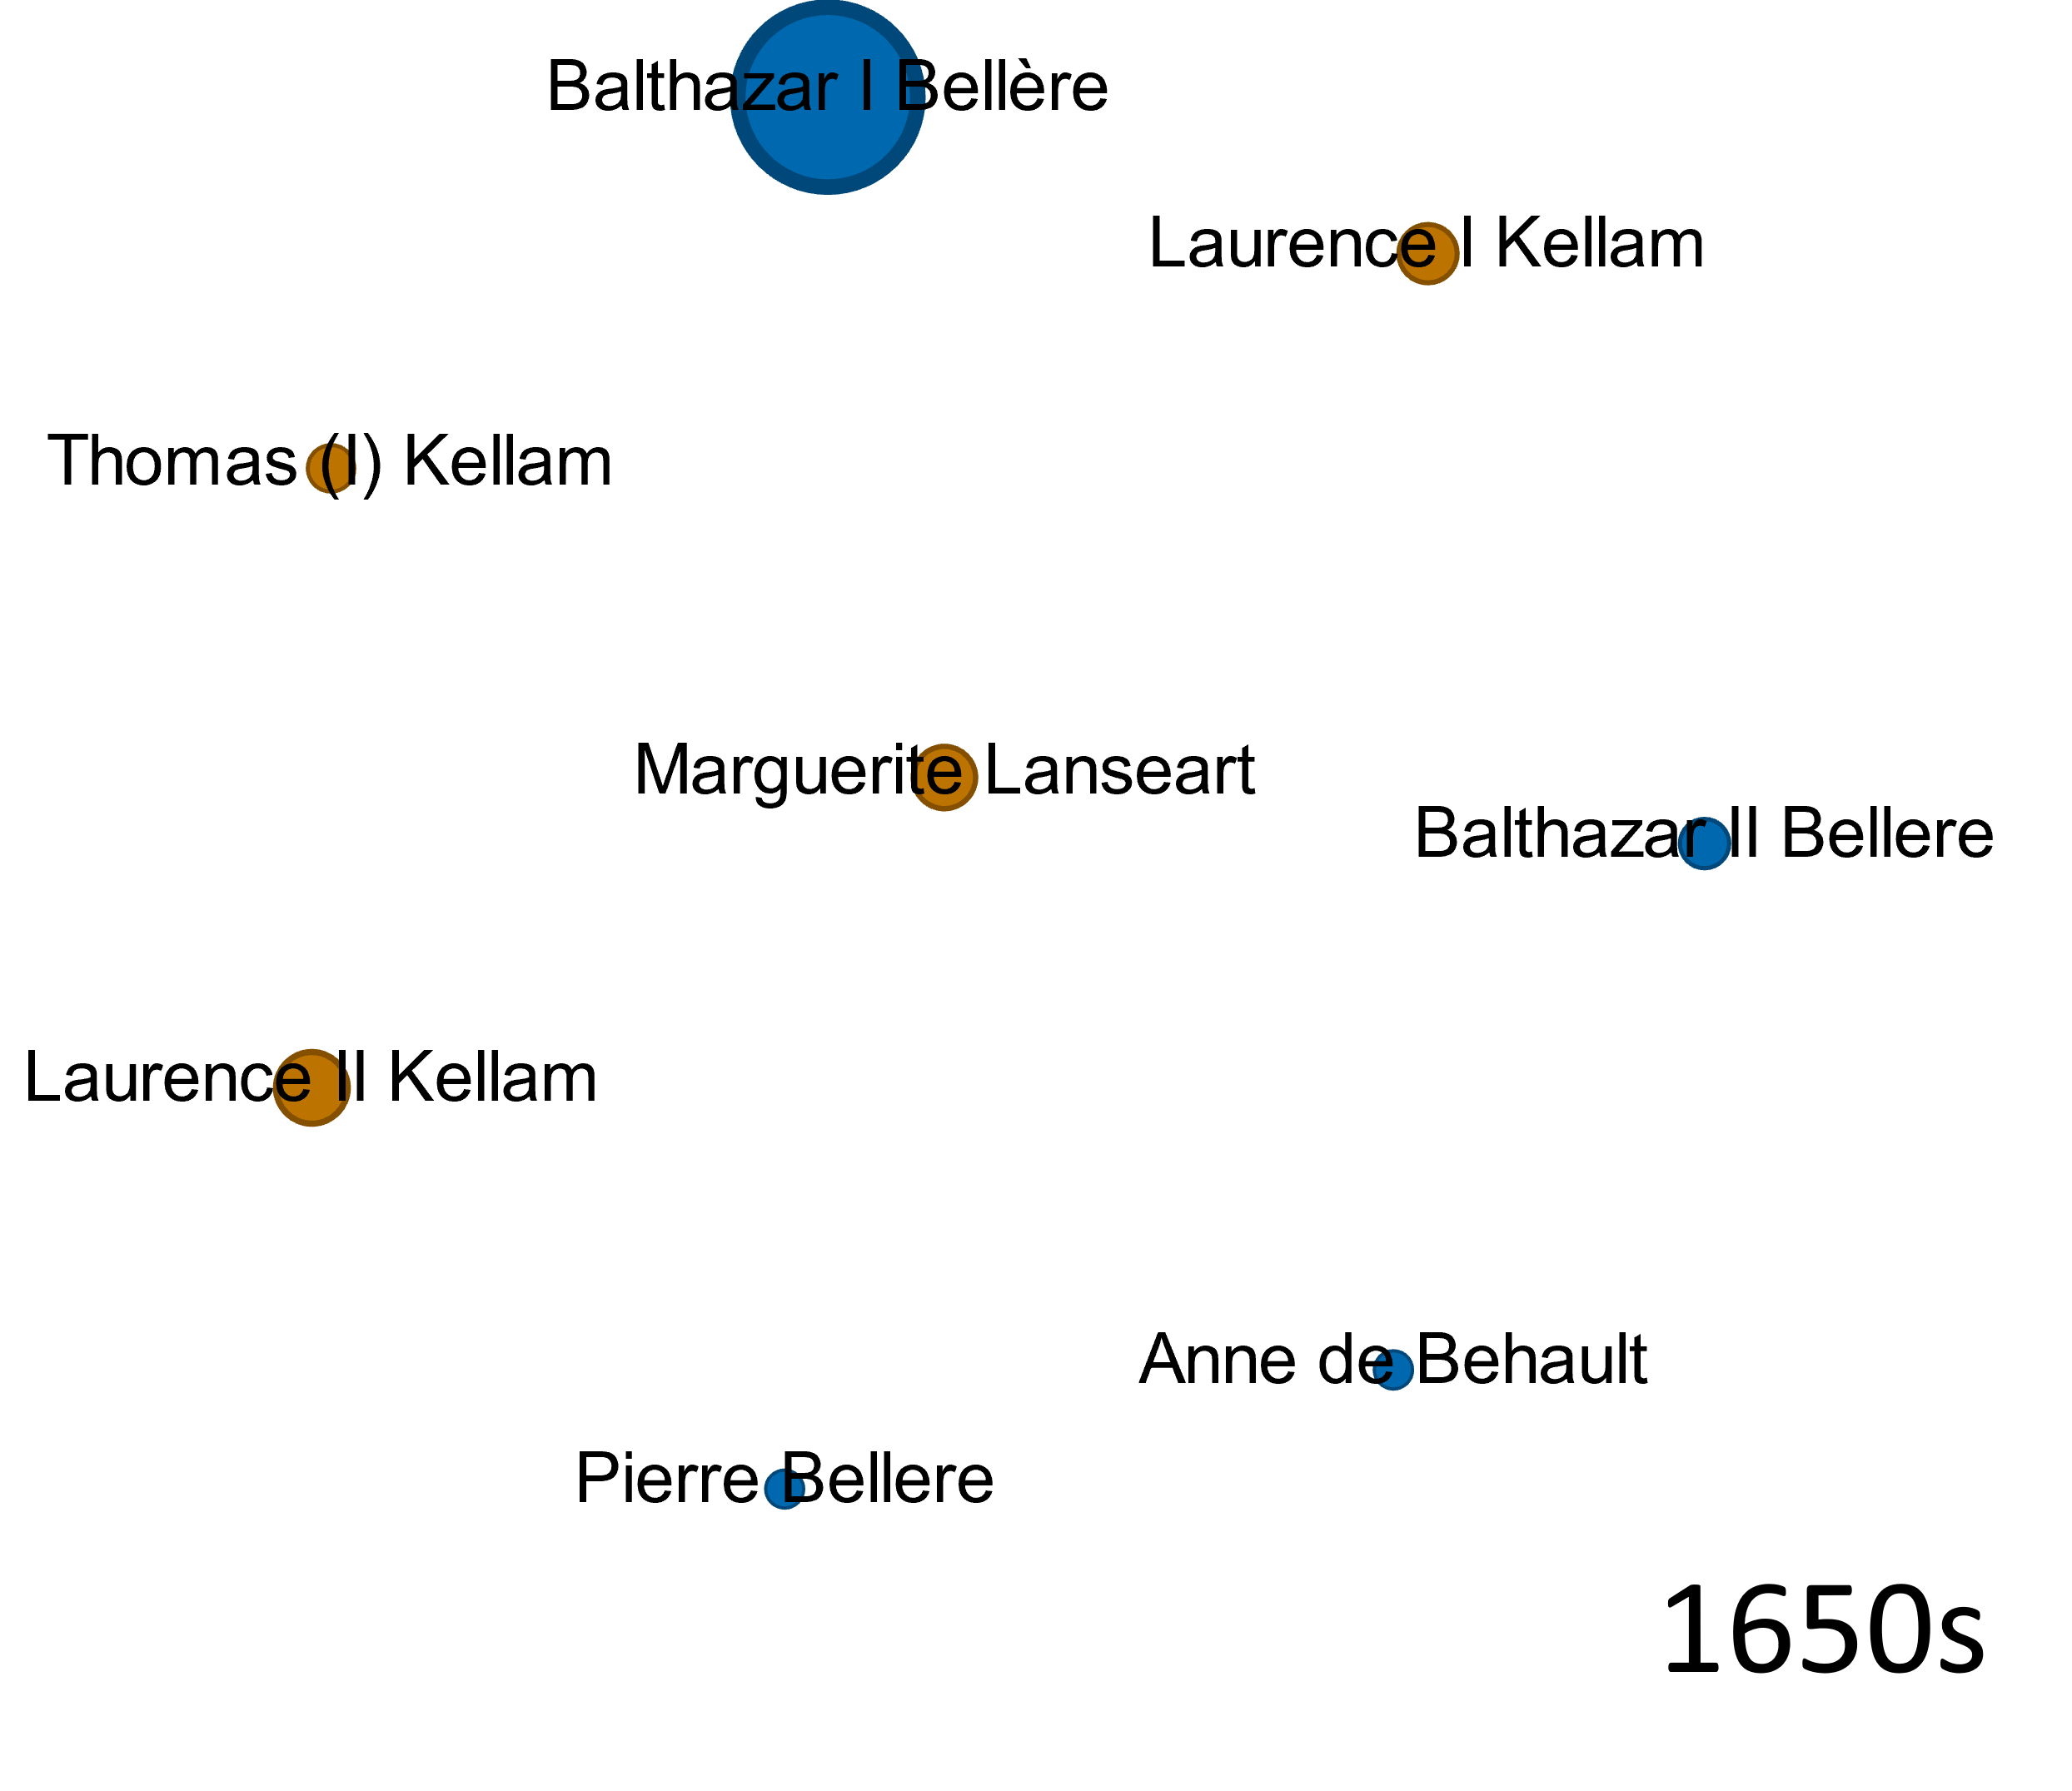
\includegraphics[scale=0.32]{graph/B&K_1650s.png}
\caption{Interaction between Printing Houses of Bellère and Kellam}
\label{fig:interactionBelAndKel}
\end{figure}

\pagebreak
\section{Women Printer/Publisher}
From the previous section, you may already notice that women in the Douai publishing industry showed a strange pattern. For example, in Table \ref{tab:top5Degree}, the only female among the top 5 influencers, Christine De Roovere, has a strangely lower Eigenvector Centrality than others among the top 5. Furthermore, in Table \ref{tab:modularityClass}, Marguerite Lanseart is grouped into a Modularity Class different from her own printing houses. Women might have been unique to the industry, and the mission of this section is to portray their participation through Social Network Analysis. There are 12 female printers/publishers identified\footnote{Special thanks to Prof. Soen for providing a pre-organised list.} in the dataset. Figure \ref{tab:womenMetrics} marks all the identified female printers/publishers on the People Network, and Table \ref{tab:womenMetrics} provides the details of their metrics in the Network.

\begin{figure}[H]
\centering
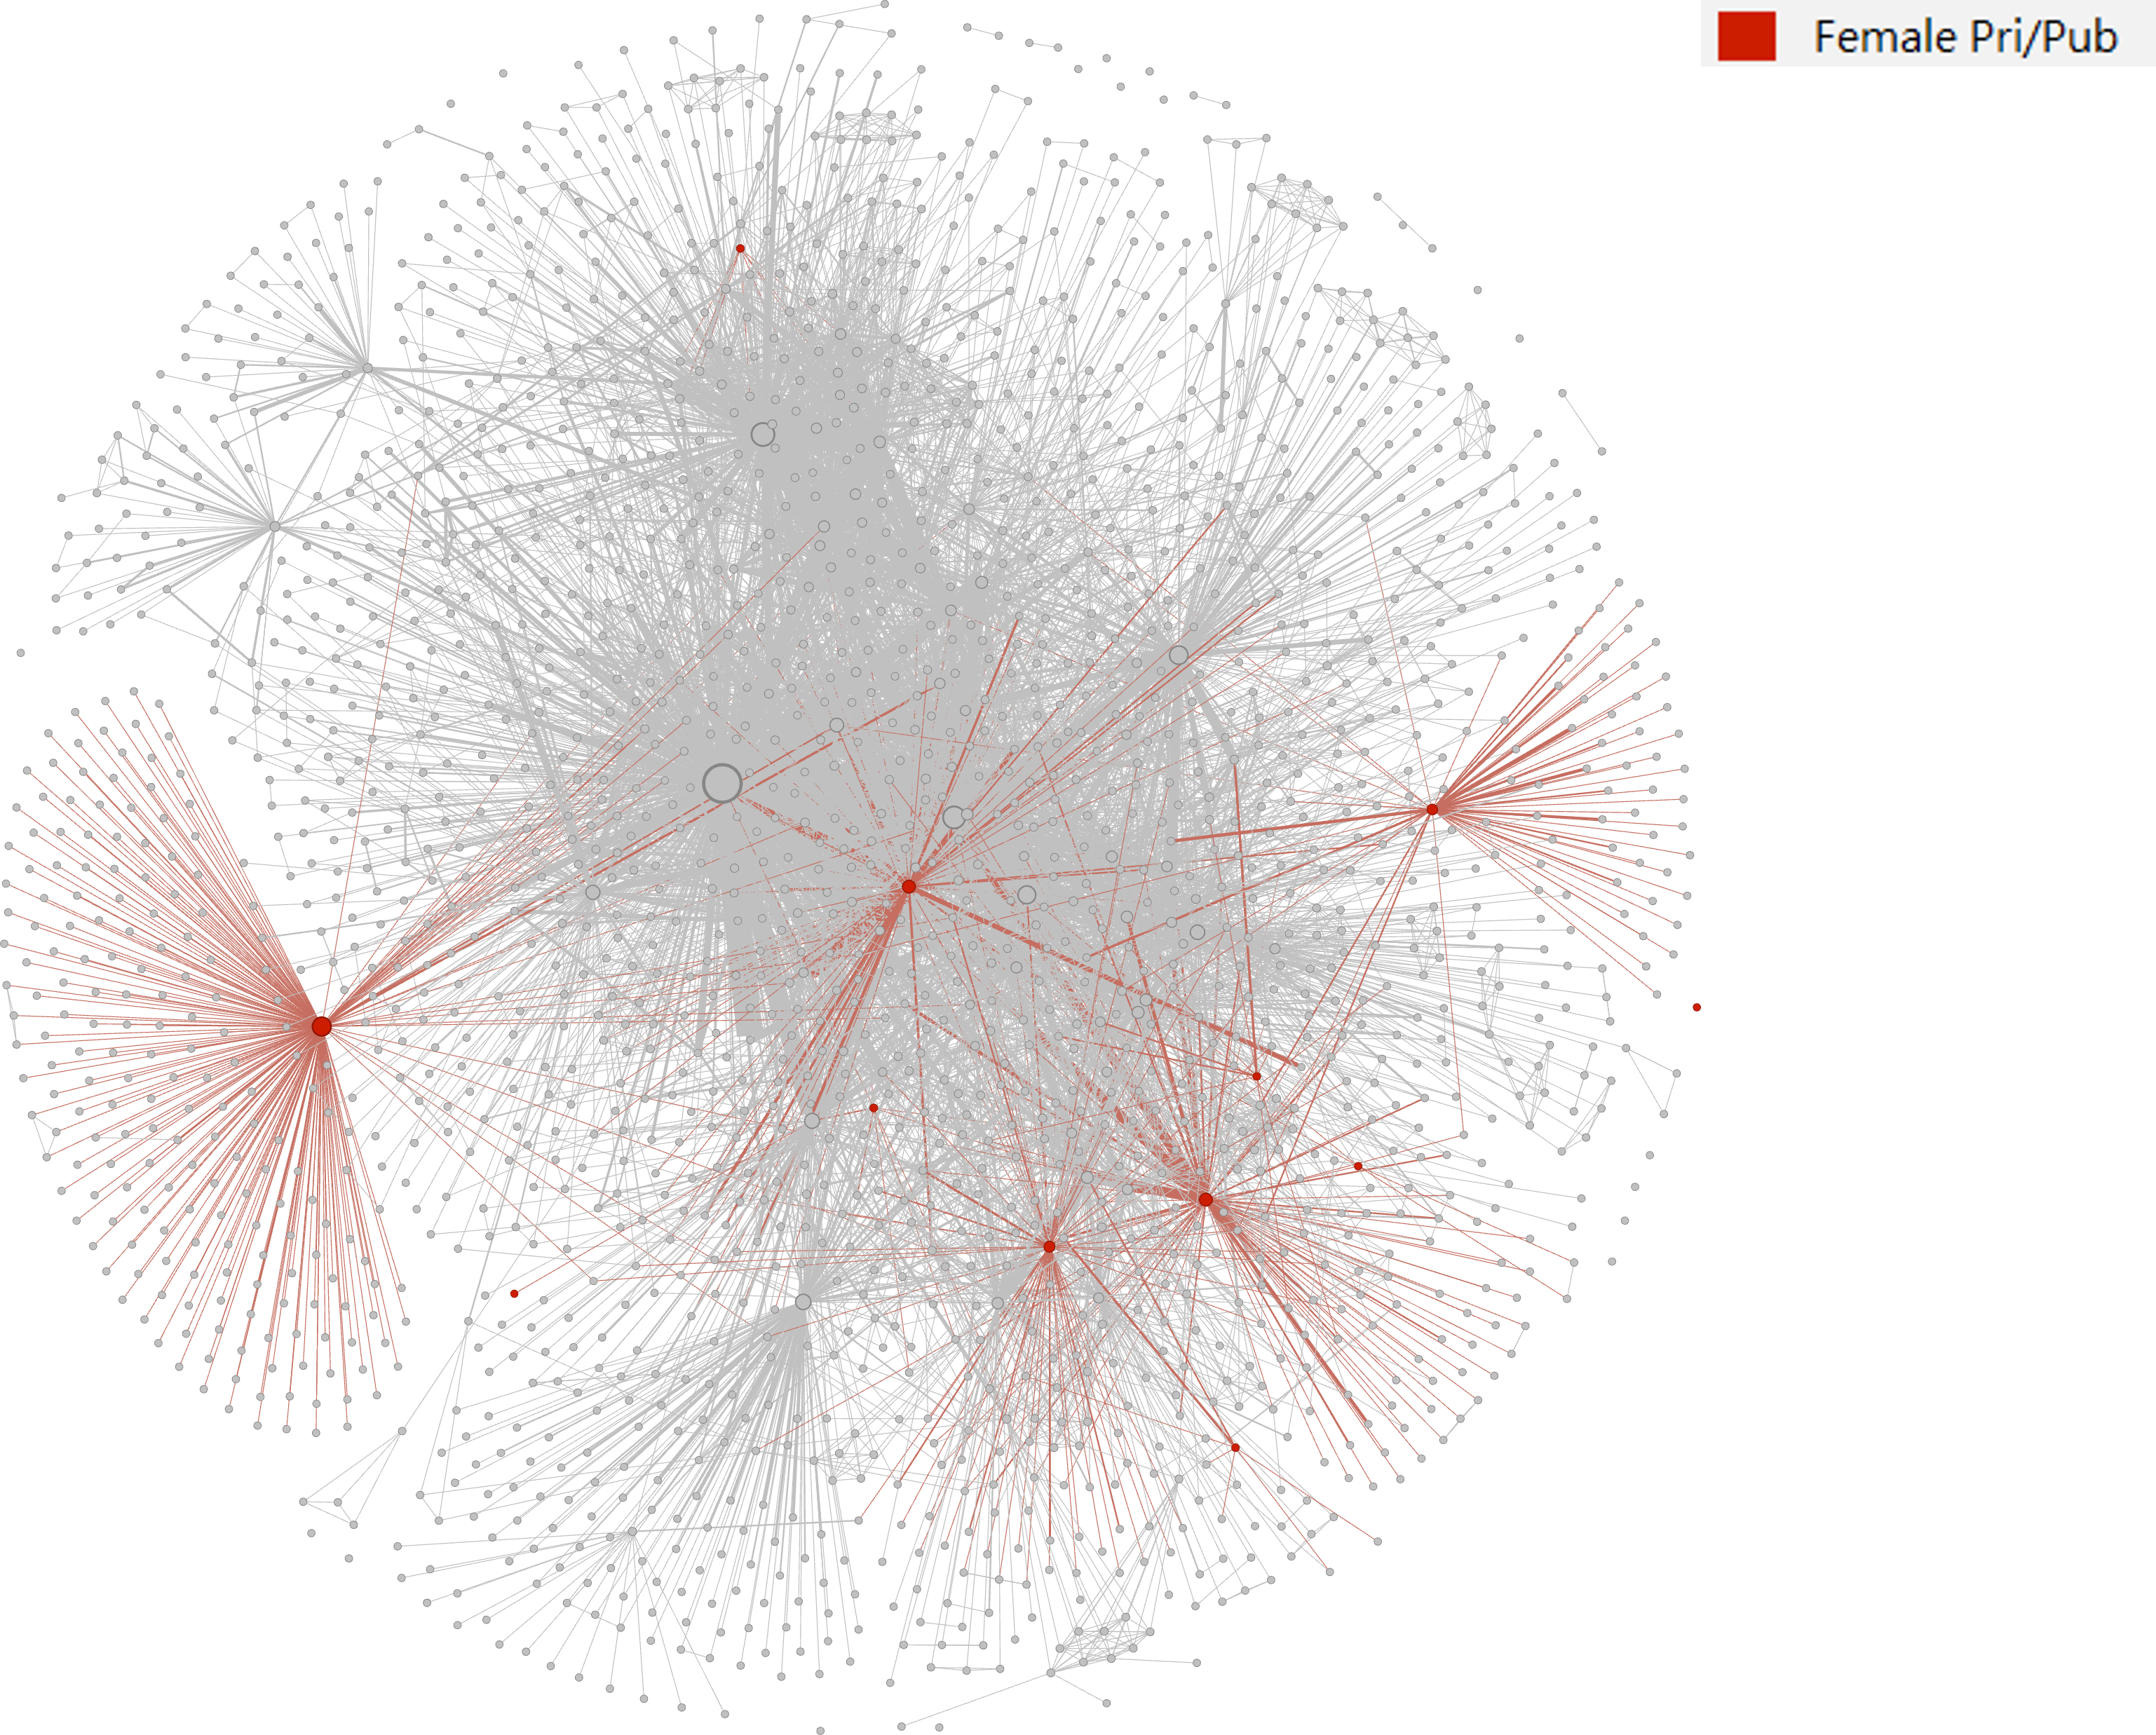
\includegraphics[scale=0.45]{graph/Women in the People Network.png}
\caption{Women Printer/Publisher (Red) in the People Network}
\label{fig:womenNet}
\end{figure}

\begin{table}[H]
\centering
\caption{Women’s Metrics in the People Network}
\label{tab:womenMetrics}
\resizebox{\textwidth}{!}{
\begin{tabular}{l|ccccc}
\multicolumn{1}{c|}{\textbf{Name}} & \textbf{Degree} & \textbf{Betweenness} & \textbf{Closeness} & \textbf{Clustering} & \textbf{Eigenvector} \\ \hline
Christine De Roovere               & 218             & 0.1752               & 0.41               & 0.00                & 0.05                 \\
Marguerite Lanseart                & 107             & 0.0209               & 0.40               & 0.08                & 0.11                 \\
Marie Vanderpiet                   & 106             & 0.0470               & 0.37               & 0.03                & 0.06                 \\
Jeanne de Menin                    & 71              & 0.0285               & 0.37               & 0.06                & 0.05                 \\
Gertrud Heusch                     & 64              & 0.0436               & 0.33               & 0.00                & 0.01                 \\
Anne de Behault                    & 9               & 0.0001               & 0.36               & 0.53                & 0.02                 \\
Dorothée Boscard                   & 9               & 0.0003               & 0.30               & 0.11                & 0.01                 \\
Widow Lodewijk De Winde            & 8               & 0.0000               & 0.29               & 1.00                & 0.01                 \\
Marie Marquette                    & 7               & 0.0015               & 0.29               & 0.29                & 0.00                 \\
Françoise Pinchon                  & 5               & 0.0019               & 0.32               & 0.40                & 0.01                 \\
Jeanne Burée                       & 1               & 0.0000               & 0.29               & 0.00                & 0.00                 \\
Widow Antoine Dieulot              & 0               & 0.0000               & 0.00               & 0.00                & 0.00                
\end{tabular}
}
\end{table}

You can notice a distinct subnetwork (Figure \ref{fig:christineDeRoovere}) at the bottom left of the whole Network. This is the connection of the female printer who has the highest Degree among women, Christine De Roovere. It seems that her collaboration was mainly with individuals that were outsiders to the industry. This explains why Christine De Roovere, with the fourth best Degrees among the whole Network, had a relatively low Eigenvector Centrality (influence) because her main connection was not with the core figures in the Network\footnote{At the meeting with Prof. Soen on 26 Apr. 2023, she explained that this may be because Christine De Roovere printed a lot of student’s work to earn fast money, and students were obviously not the core members of the industry.}.

\begin{figure}[H]
\centering
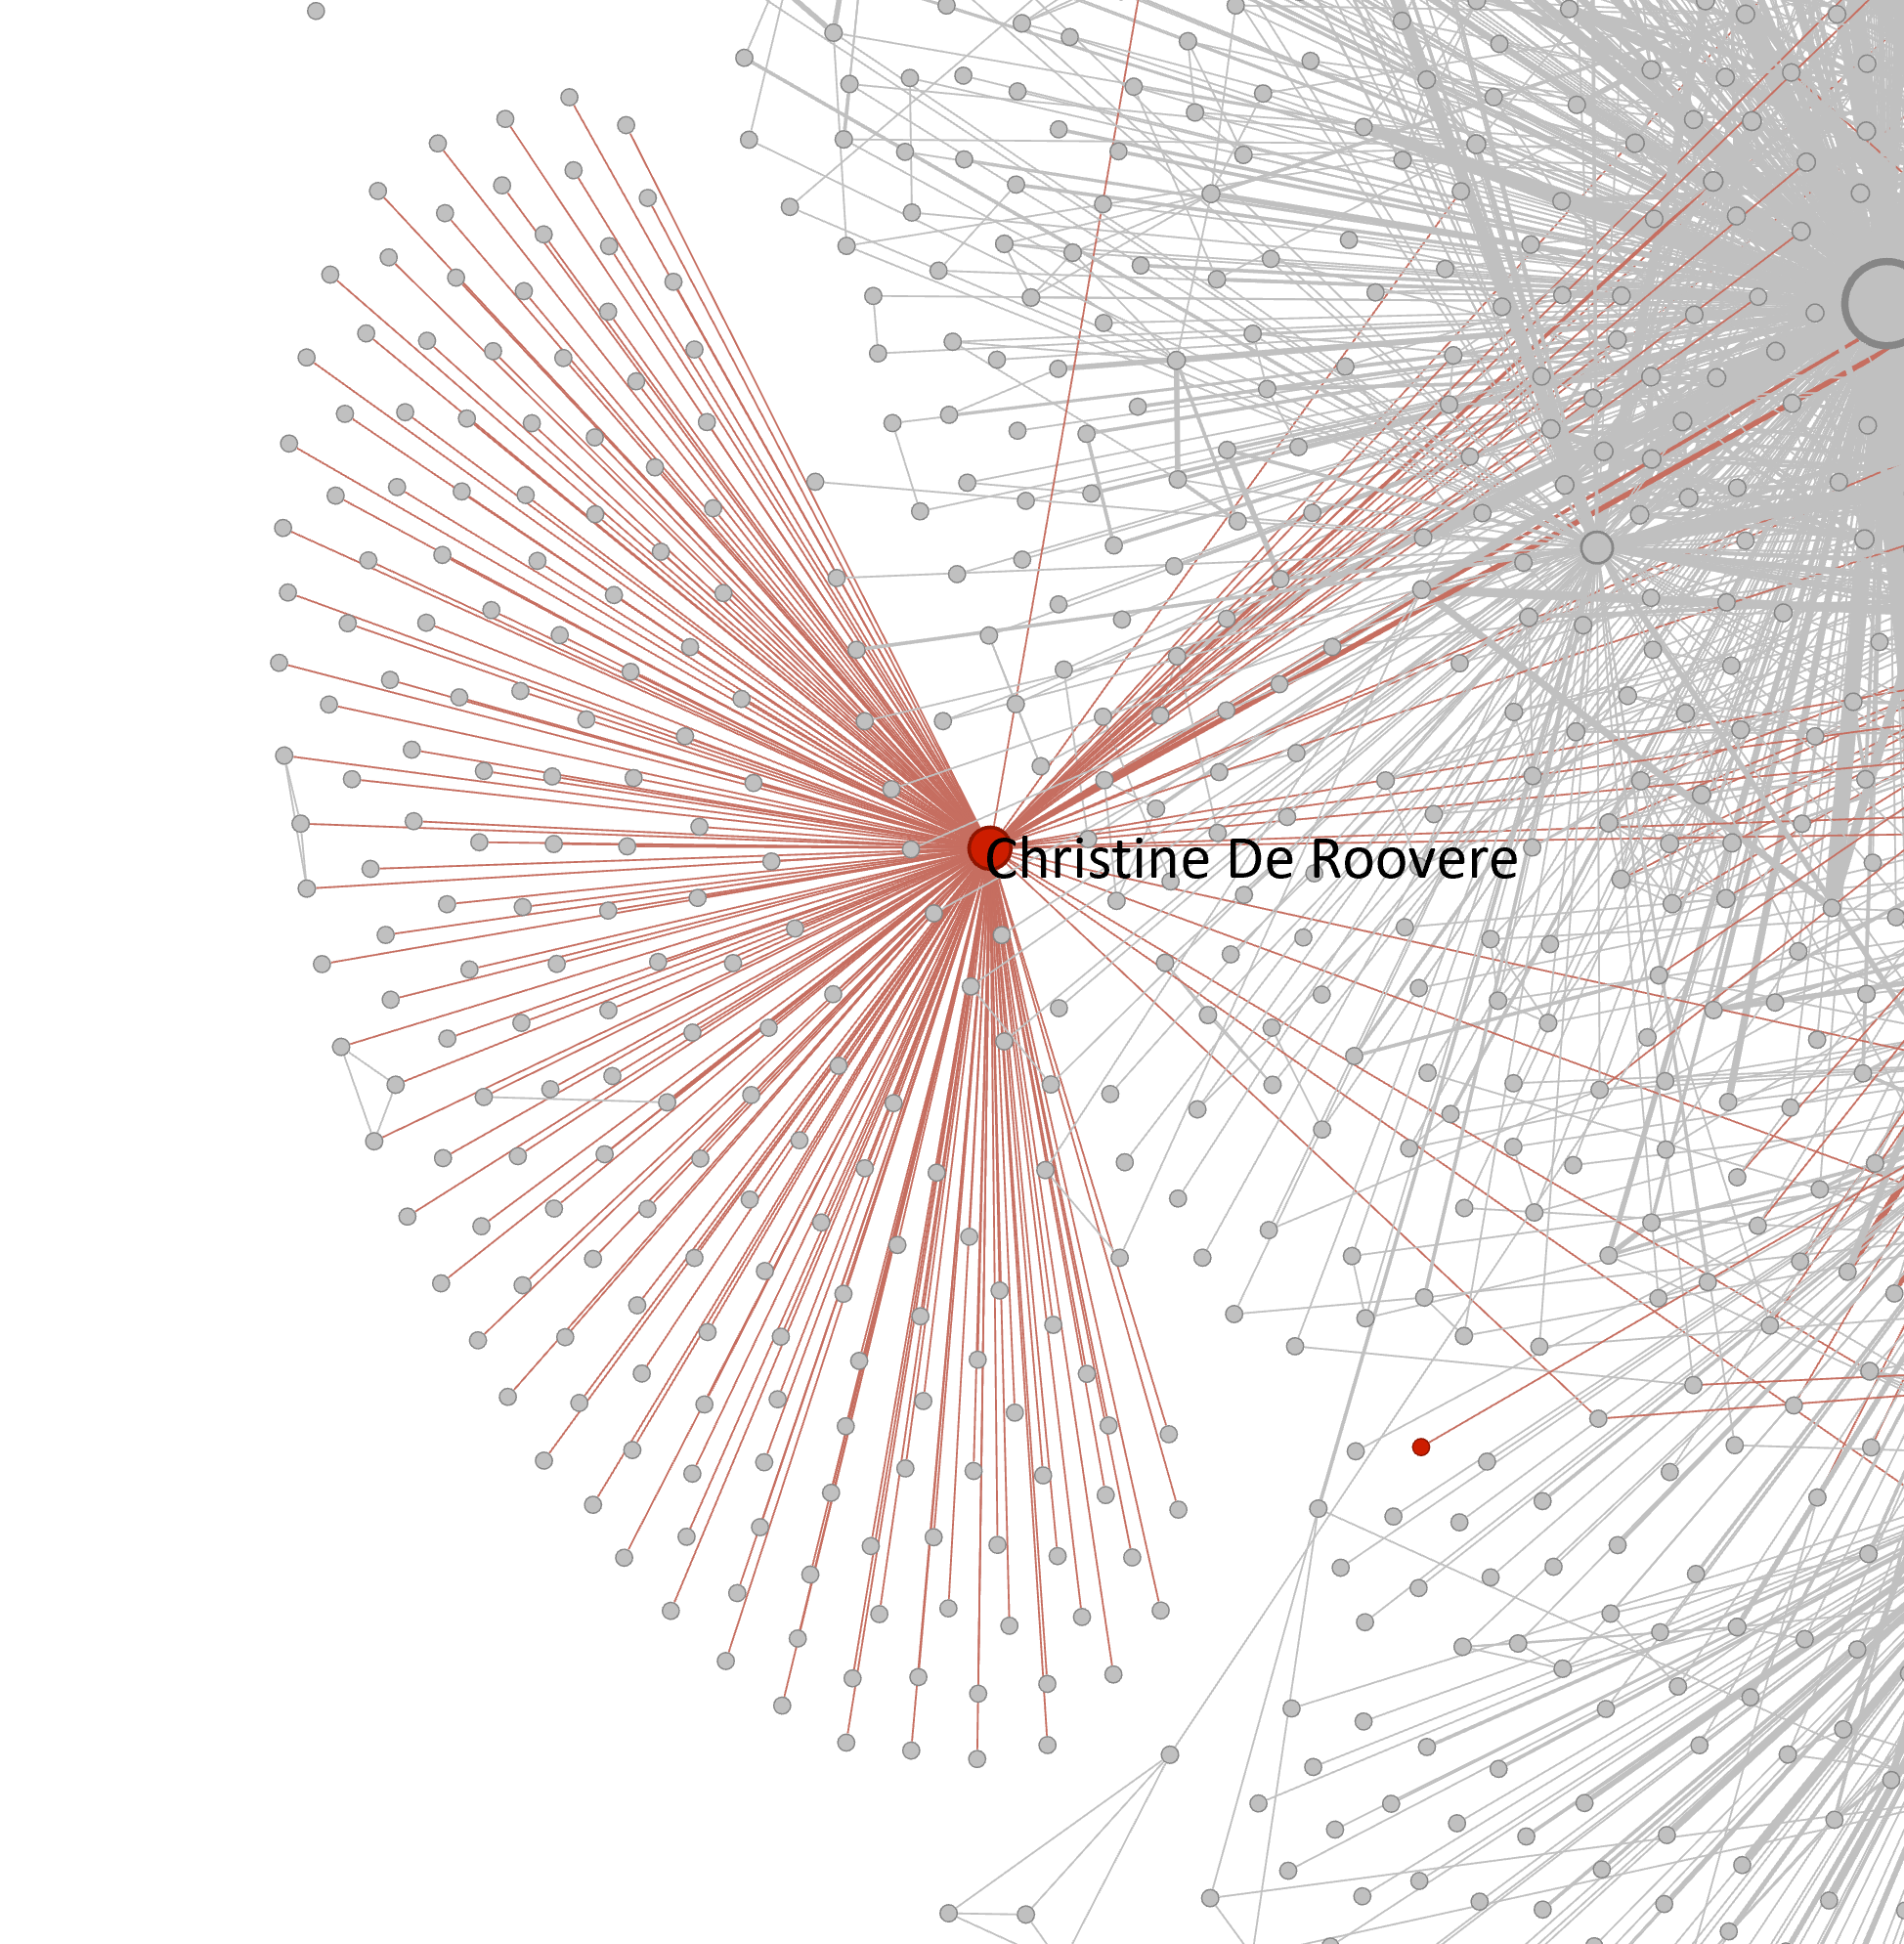
\includegraphics[scale=0.6]{graph/Christine De Roovere.png}
\caption{The connection of Christine De Roovere}
\label{fig:christineDeRoovere}
\end{figure}

Simply showing the metrics of female printers/publishers cannot provide enough information about women’s involvement in the industry. We can conduct further calculations to get a clearer vision. Firstly, we draw a picture of women’s participation (Degree Centrality) through time (Figure \ref{fig:womenDegree}). Female printers/publishers seem to be more active after the 1600s, later than males. However, after the 1600s, both female and male Degree Centrality maintained the same level till the end. This could justify the historian’s claim that in early modern Europe, females contributed the same to the publishing industry as males (Wyffels, 2021).

\begin{figure}[H]
\centering
\includegraphics[scale=0.4]{graph/Trend of Women’s Degree Centrality.png}
\caption{Trend of Female and Male Printer/Publisher’s Degree Centrality}
\label{fig:womenDegree}
\end{figure}

Secondly, we can compare the mean metrics of female printers/publishers with males. The Clustering Coefficient determines how well-connected a node’s neighbours are (Carrington \& Scott, 2011; Wasserman \& Faust, 1994). Female printers/publishers having a lower Clustering Coefficient could show the situation that women’s opportunities were limited (Wyffels, 2021), so they were less possible to be in the group with the core active members of the industry. On the other hand, female printers/publishers have a higher Betweenness Centrality. Since Betweenness Centrality compute how well a node serves as a bridge for others to connect, this could reflect the history that women often entered a printing house from another through marriage and this marriage became the collaboration of the two printing houses (Wyffels, 2021).

\begin{table}[H]
\centering
\caption{Cross Table of Mean Metrics of Female and Male Printers/Publishers}
\label{tab:crossFandM}
\begin{tabular}{lcc}
\multicolumn{1}{l|}{}                       & \textbf{Female}               & \textbf{Male}                 \\ \hline
\multicolumn{1}{l|}{\textit{n}}             & \textit{10\tablefootnote{Two people are eliminated. The first is Christine De Roovere, since her Degree is two times higher than the one ranked the second, it makes her an outlier. The second is Widow Antoine Dieulot, who only printed one publication and did not connect to anyone else which makes her metrics all 0. Putting her in the analysis may inaccurately make the overall female metrics lower.}}                   & \textit{87\tablefootnote{Balthazar I Bellère is eliminated from this comparison because his Degree is almost two times higher than the one ranked the second, making him an obvious outlier. Putting him in could make the overall male metrics inaccurately higher.}}                   \\ \hline
\multicolumn{1}{l|}{Degree Centrality}      & 0.0188                        & 0.0128                        \\
\multicolumn{1}{l|}{Eigenvector Centrality} & 0.0277                        & 0.0202                        \\
\multicolumn{1}{l|}{Clustering Coefficient} & 0.2504                        & {\color[HTML]{CB0000} 0.5222} \\
\multicolumn{1}{l|}{Closeness Centrality}   & 0.3327                        & 0.2994                        \\
\multicolumn{1}{l|}{Betweenness Centrality} & {\color[HTML]{CB0000} 0.0144} & 0.0082                        \\ \hline
\multicolumn{3}{l}{* {\color[HTML]{CB0000} Red numbers} are significantly higher.\tablefootnote{By t-test. Clustering Coefficient: t=--2.22, p=0.03; Betweenness Centrality: t=-2.57, p=0.01.}}                           
\end{tabular}
\end{table}

\counterwithout{footnote}{chapter}
\chapter{Different Approaches to Network}
\label{differentNetwork}
In Chapter \ref{languages} and Chapter \ref{influencers}, the Network we built was based on people involved in the same publications. In this chapter, we approach different methods to build the Network and explore the possible benefits.

\section{The Publication Network}
Since the printing house of Kellam was the long-lasting English printing house in Douai, scholars have shown their interest in understanding its development. It has been observed that the success of the Kellam printing house might be thanks to their switching printing strategy (Soetaert \& Wyffels, 2021). Specifically, to fulfil the market needs, the Kellam printing house gradually participated in more languages so they could reach a broader audience from the European continent. It can be interesting to illustrate the switching of Kellam’s participation on the Network. Nonetheless, it can be hard to illustrate it with the People Network built in Chapter \ref{languages}. We only want to see the dynamic of the Kellams. However, if we filter out the nodes that do not belong to the Kallam printing house, the house’s connection with other nodes would be gone. If we keep all the nodes, there would be too many edges that are not relevant. To solve this problem, we can build the Network in the opposite direction. In other words, this time, each node is a publication, and the edge connecting the two nodes is the person who participated in both publications.

\begin{figure}[H]
\centering
\includesvg[scale=1.1]{graph/An Example of Edge in Publication Network.svg}
\caption{An Example of Edge in the Publication Network}
\label{fig:examplePubNet}
\end{figure}

\pagebreak
By filtering out the edges of people that do not belong to the Kellam printing house, we can have a Network of publications published by the Kellams. In Figure \ref{fig:pubNet} you can see that the graph has already divided the Network into three groups, which can represent the publishing strategies of the Kellams in three generations. Since edges represent different persons and we are only interested in the diversity of languages in publications Kellams had published, we can just focus on the nodes in the graph.

\begin{figure}[H]
\centering
\includegraphics[scale=0.45]{graph/The Publication Network Only Published by Kellam.png}
\caption{The Publication Network Only Published by Kellam}
\label{fig:pubNet}
\end{figure}

Figure \ref{fig:laurenceI} shows the publication published by the first generation, Laurence I Kellam. You can see that almost half of the nodes are English, indicating during this time (in the early 1600s) Laurence I Kellam still had a strong connection with his homeland, England, and English publications were important business to the printing house.

\begin{figure}[H]
\centering
\includesvg[scale=0.35]{graph/Kellam_gen1.svg}
\caption{Publications Published by Laurence I Kellam}
\label{fig:laurenceI}
\end{figure}

However, moving to the second generation (Figure \ref{fig:margueriteAndThomas}) after the death of Laurence I Kellam (1612) (Soetaert, 2020a), Laurence I Kellam’s wife Marguerite Lanseart and eldest son Thomas (I) Kellam continued the printing house (Soetaert, 2018a; Soetaert et al., 2023b). The Latin nodes occupy the biggest portion suggesting that the printing house focused on the business of Latin publications during this time. Since Marguerite Lanseart was a native of the Low Countries (Soetaert et al., 2023b) and Thomas (I) Kellam was also born here (Soetaert, 2018a), it is understandable that their connection with the English could be weaker.

\begin{figure}[H]
\centering
\includesvg[scale=0.4]{graph/Kellam_gen2.svg}
\caption{Publications Published by Marguerite Lanseart and Thomas (I) Kellam}
\label{fig:margueriteAndThomas}
\end{figure}

After the death of Thomas (I) Kellam (1620) (Soetaert, 2018a) and Marguerite Lanseart (1623) (Soetaert et al., 2023b), Laurence II Kellam took over the printing house (Soetaert, 2020a) and entered the third generation. You can notice that the nodes are more colourful than the last generation, showing that Laurence II Kellam indeed applied different strategies for their business and collaborated with more diverse communities.

\begin{figure}[H]
\centering
\includesvg[scale=0.35]{graph/Kellam_gen3.svg}
\caption{Publications Published by Laurence II Kellam}
\label{fig:laurenceII}
\end{figure}

\section{The Compiler/Editor/Revisor Network}
Compilers/Editors/Revisors played a significant role during the production of publications (Soetaert \& Wyffels, 2021). They shaped the content and ensured the quality of the final product, which made them work closely with printers/publishers. Constructing the Network of Compilers/Editors/Revisors can provide a deep understanding of the Douai publishing industry. However, since many publications may only have one Compiler/Editor/Revisor, it can be hard to create their connection with the People Network from Chapter \ref{languages}. Therefore, we use another approach to draw their connection.

Instead of using the same publication as an edge, this time we use the same printer/publisher. Specifically, if the two Compilers/Editors/Revisors had been involved in publications that had been published by the same printer/publisher, they would be connected in the Network. In the end, there are 127 nodes and 2305 edges in the Network. Since there is no printer/publisher only published one publication or collaborated with only one Compiler/Editor/Revisor, all the nodes in the Network have an edge.

\begin{figure}[H]
\centering
\includesvg[scale=0.85]{graph/An Example of Edge in CER Network.svg}
\caption{An Example of Edge in the Compiler/Editor/Revisor Network}
\label{fig:exampleCERNet}
\end{figure}

Figure \ref{fig:CERNet} shows the Compiler/Editor/Revisor Network. With the edges marked with the printing house they belonged to; it can be noticed that each printing house seemed to have its long-term collaborative Compilers/Editors/Revisors since the Network can be well-divided by the colours. Yellow nodes, which all have a Degree higher than 61, are the few who have worked with different printing houses (26 out of 127), indicating that they could be influential Compilers/Editors/Revisors in the industry.

The one that has the highest Degree (Table \ref{tab:top5CER}) in this Network is Richard Gibbons, who was a English priest and a professor at the University of Douai. This again proves the influence of English Catholics on the Douai publishing industry.

\begin{table}[H]
\centering
\caption{Top 5 Degrees in the Compiler/Editor/Revisor Network}
\label{tab:top5CER}
\resizebox{\textwidth}{!}{
\begin{tabular}{l|ccccc}
\multicolumn{1}{c|}{\textbf{Name}} & \textbf{Degree} & \textbf{Betweenness} & \textbf{Closeness} & \textbf{Clustering} & \textbf{Eigenvector} \\ \hline
Richard Gibbons                    & 95              & 0.0969               & 0.76               & 0.45                & 0.13                 \\
Georges Colveneere                 & 93              & 0.0841               & 0.78               & 0.48                & 0.13                 \\
Henri de Sommal                    & 92              & 0.1069               & 0.77               & 0.49                & 0.13                 \\
François Sylvius                   & 89              & 0.1002               & 0.76               & 0.51                & 0.13                 \\
Nicolas de Leuze                   & 78              & 0.0295               & 0.70               & 0.65                & 0.13                
\end{tabular}
}
\end{table}

\begin{figure}[H]
\centering
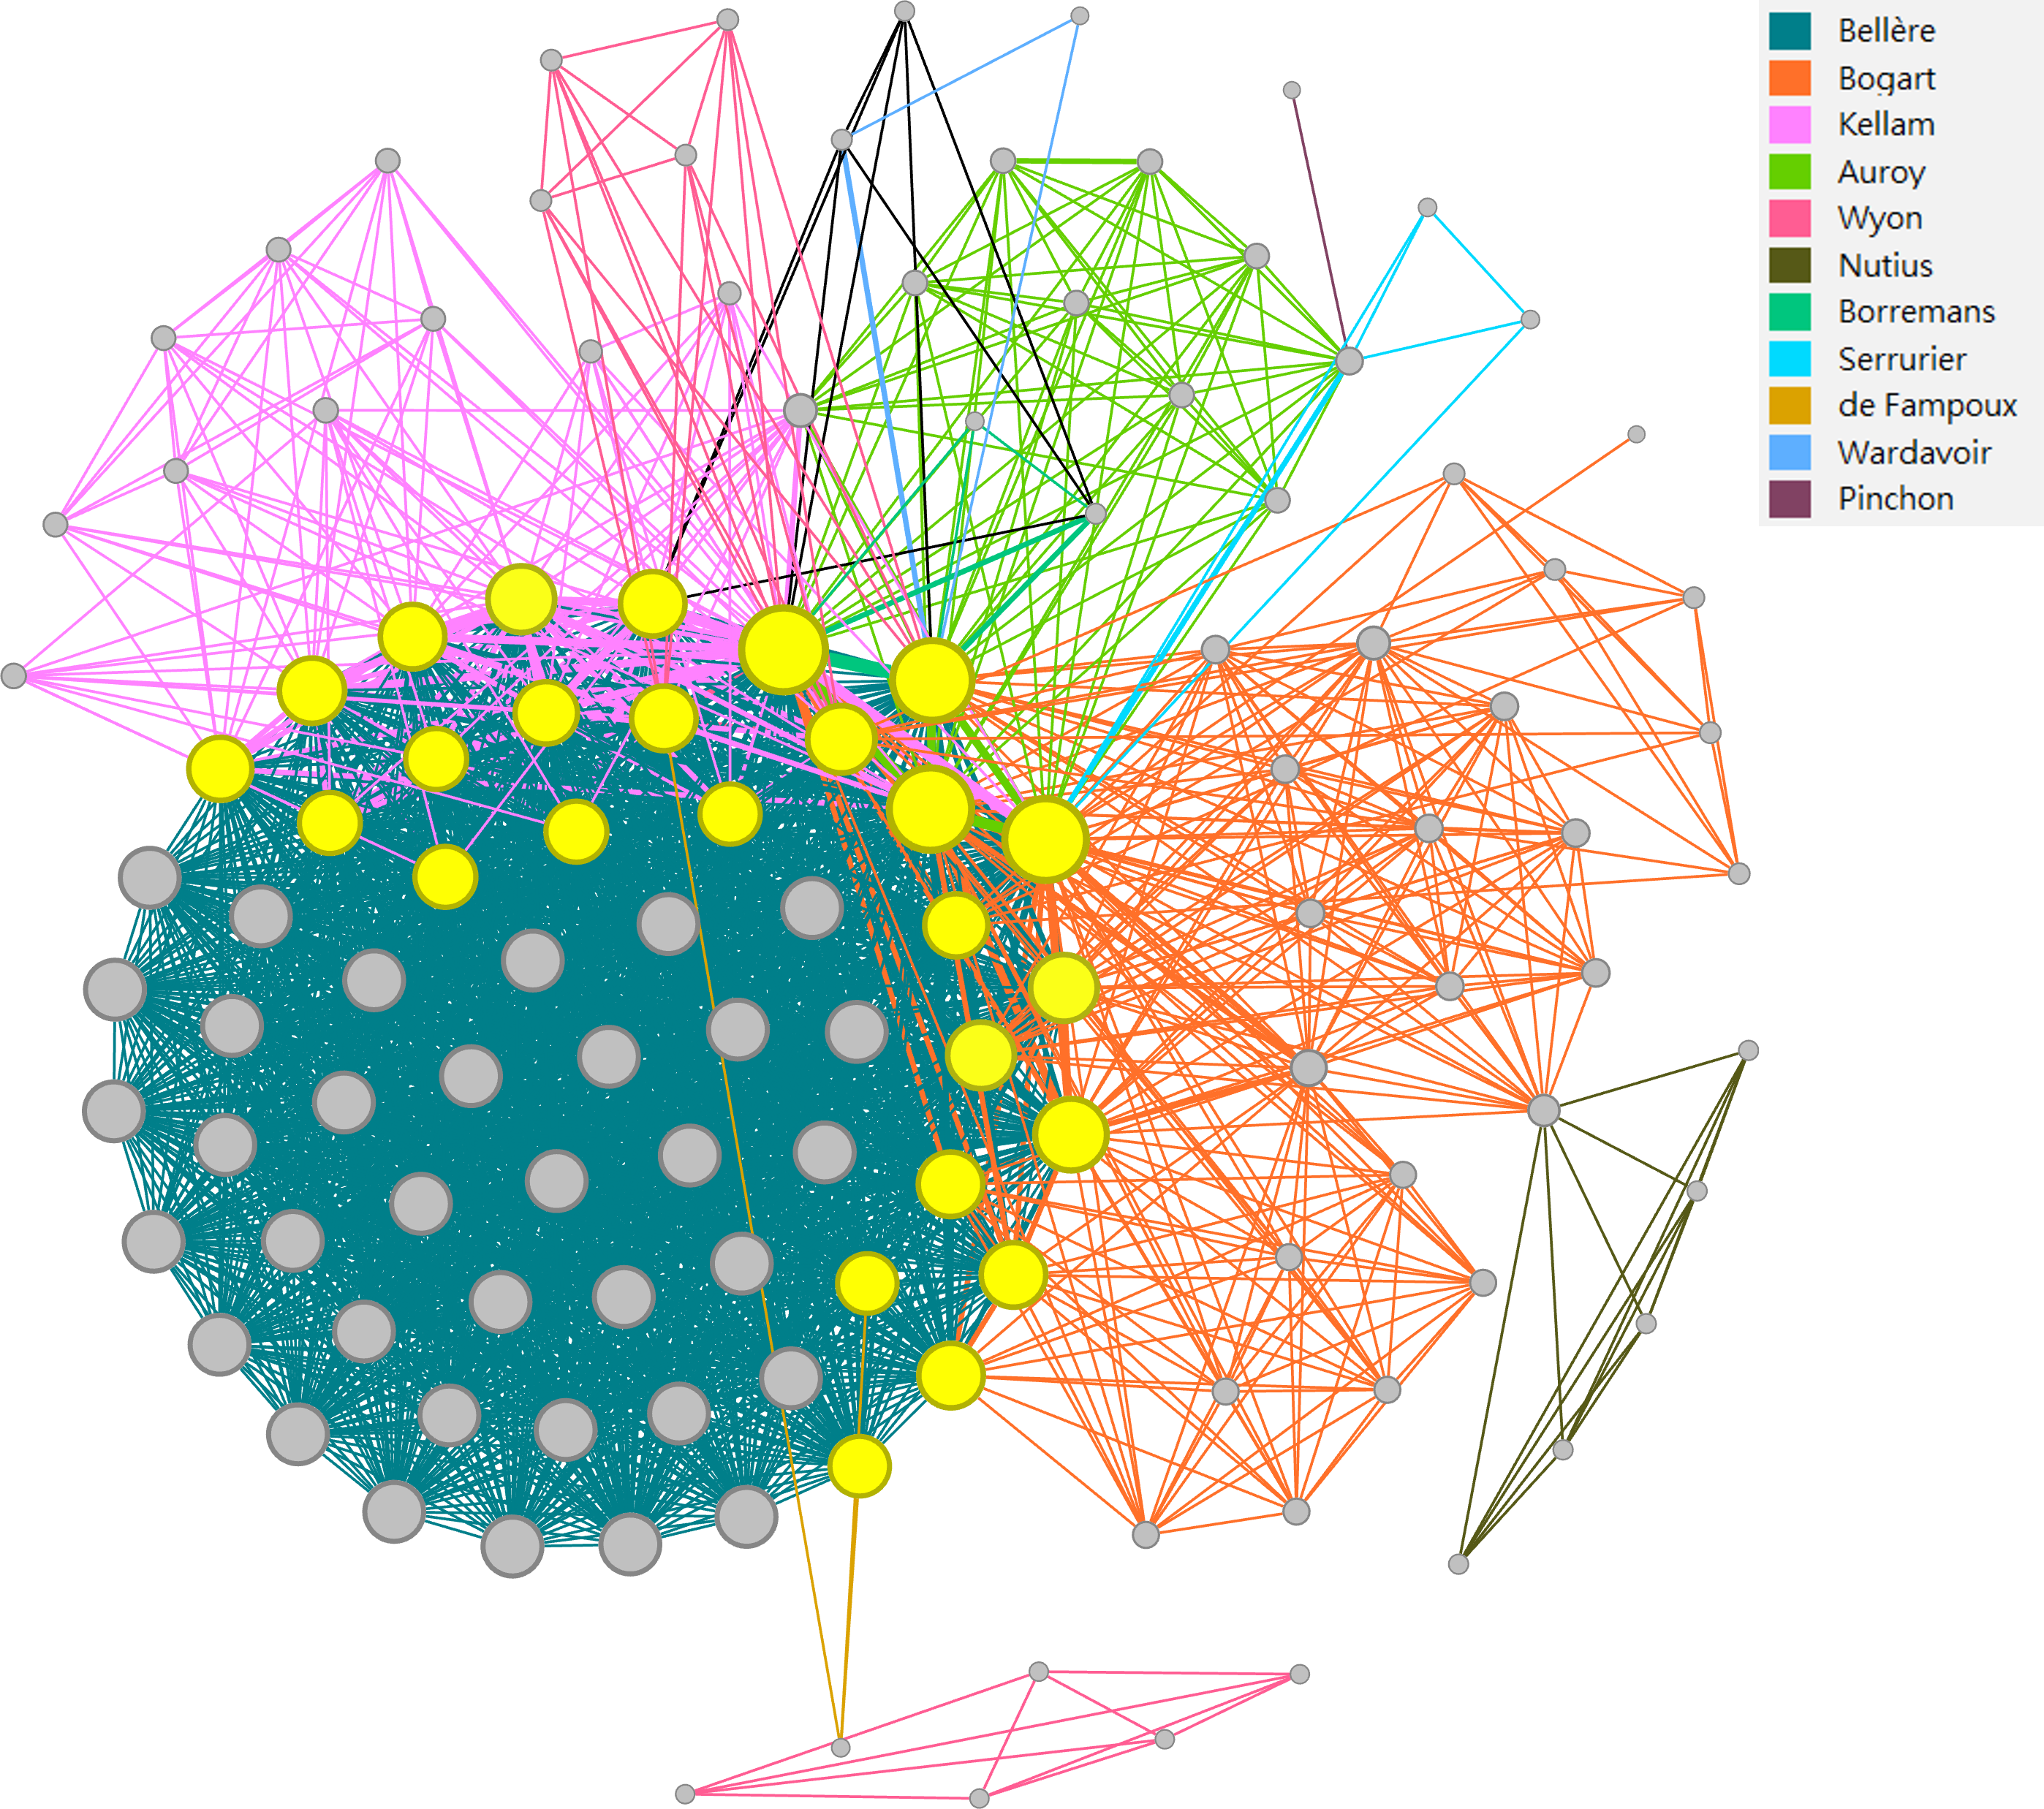
\includegraphics[scale=0.6]{graph/CER Published by the Same PP.png}
\caption{The Compiler/Editor/Revisor Network}
\label{fig:CERNet}
\end{figure}

\counterwithout{footnote}{chapter}
\chapter{Sharing the Network}
\label{shareNetwork}
In the previous chapters, you can see many graphs of Networks. Nevertheless, Networks are often complicated, and graphs can be too small for detailed information. For instance, for Figure \ref{fig:CERNet}, scholars may also be interested in finding out the details of the yellow nodes. However, since marking the labels (names) of nodes can cause the graph messy and listing the details of nodes in another table can unwisely take an extensive portion of this paper, a way to share interactive Networks is needed. Gladly, with the help of a web application, Retina, it is possible to share the Networks with others for further studies.

Lots of filtering and annotating on the Networks in the previous chapters were on the edges. However, since it is not possible to filter the edges on Retina, additional adjustments to our dataset are needed. For example, to filter out a language, we can first compute the times each node (person) was involved in this language and eliminate the nodes that have a value bigger than 0. Table \ref{tab:calculateTheMost} shows examples of this computation, we conduct this on roles, languages, and periods. In addition, you can notice that we also compare the values between columns to determine the node’s “most involved”. This will be assigned to the column that has the largest value, and if there are two highest values, it will be assigned “Multi”.

\begin{table}[H]
\centering
\caption{Examples of Calculating the Most}
\label{tab:calculateTheMost}
\resizebox{\textwidth}{!}{
\begin{tabular}{l|cccccc}
\multicolumn{1}{c|}{\textbf{ODIS\_PERS\_ID}} & \textbf{…} & \textbf{heirs/widow} & \textbf{printer/publisher} & \textbf{translator} & \textbf{unspecified} & \textbf{Most Involved Role} \\ \hline
119240                                       & …0         & 0                    & 37                         & 0                   & 0                    & printer/publisher          
\end{tabular}
}
\end{table}

\begin{table}[H]
\centering
\resizebox{\textwidth}{!}{
\begin{tabular}{l|cccccc}
\multicolumn{1}{c|}{\textbf{ODIS\_PERS\_ID}} & \textbf{Dutch} & \textbf{English} & \textbf{French} & \textbf{Latin} & \textbf{Spannish} & \textbf{Most Involved Language} \\ \hline
119240                                       & 0              & 16               & 5               & 16             & 0                 & Multi                          
\end{tabular}
}
\end{table}

\begin{table}[H]
\centering
\resizebox{\textwidth}{!}{
\begin{tabular}{l|cccccccc}
\multicolumn{1}{c|}{\textbf{ODIS\_PERS\_ID}} & \textbf{...} & \textbf{1590s} & \textbf{1600s} & \textbf{1610s} & \textbf{1620s} & \textbf{1630s} & \textbf{...} & \textbf{Most Involved Period} \\ \hline
119240                                       & ...0         & 4              & 31             & 1              & 1              & 0              & 0...         & 1600s                        
\end{tabular}
}
\end{table}

\pagebreak
You can find the interactive version of Networks built from Chapter \ref{languages} and Chapter \ref{differentNetwork}.2 through the links below.
\\

To the \href{https://ouestware.gitlab.io/retina/1.0.0-beta.1/#/graph/?url=https%3A%2F%2Fgist.githubusercontent.com%2Fdodopianist%2F284997da5801f90b7767df40eef365b0%2Fraw%2Ff300443ab5160ab340f1472c63a4edd270ea1c05%2Fpeople_network.gexf&sa[]=ei&sa[]=be&sa[]=clo&sa[]=deg-n&sa[]=clu-n&ca[]=gn&ca[]=msr&ca[]=msl&ca[]=msp&ca[]=md-s&ca[]=bip&ca[]=bir&ca[]=deap&ca[]=dear&ca[]=pri&ca[]=hoo&ca[]=clo&ca[]=be&ca[]=deg-n&ca[]=clu-n&ec=o}{\underline{People Network}}.
\begin{figure}[H]
\centering
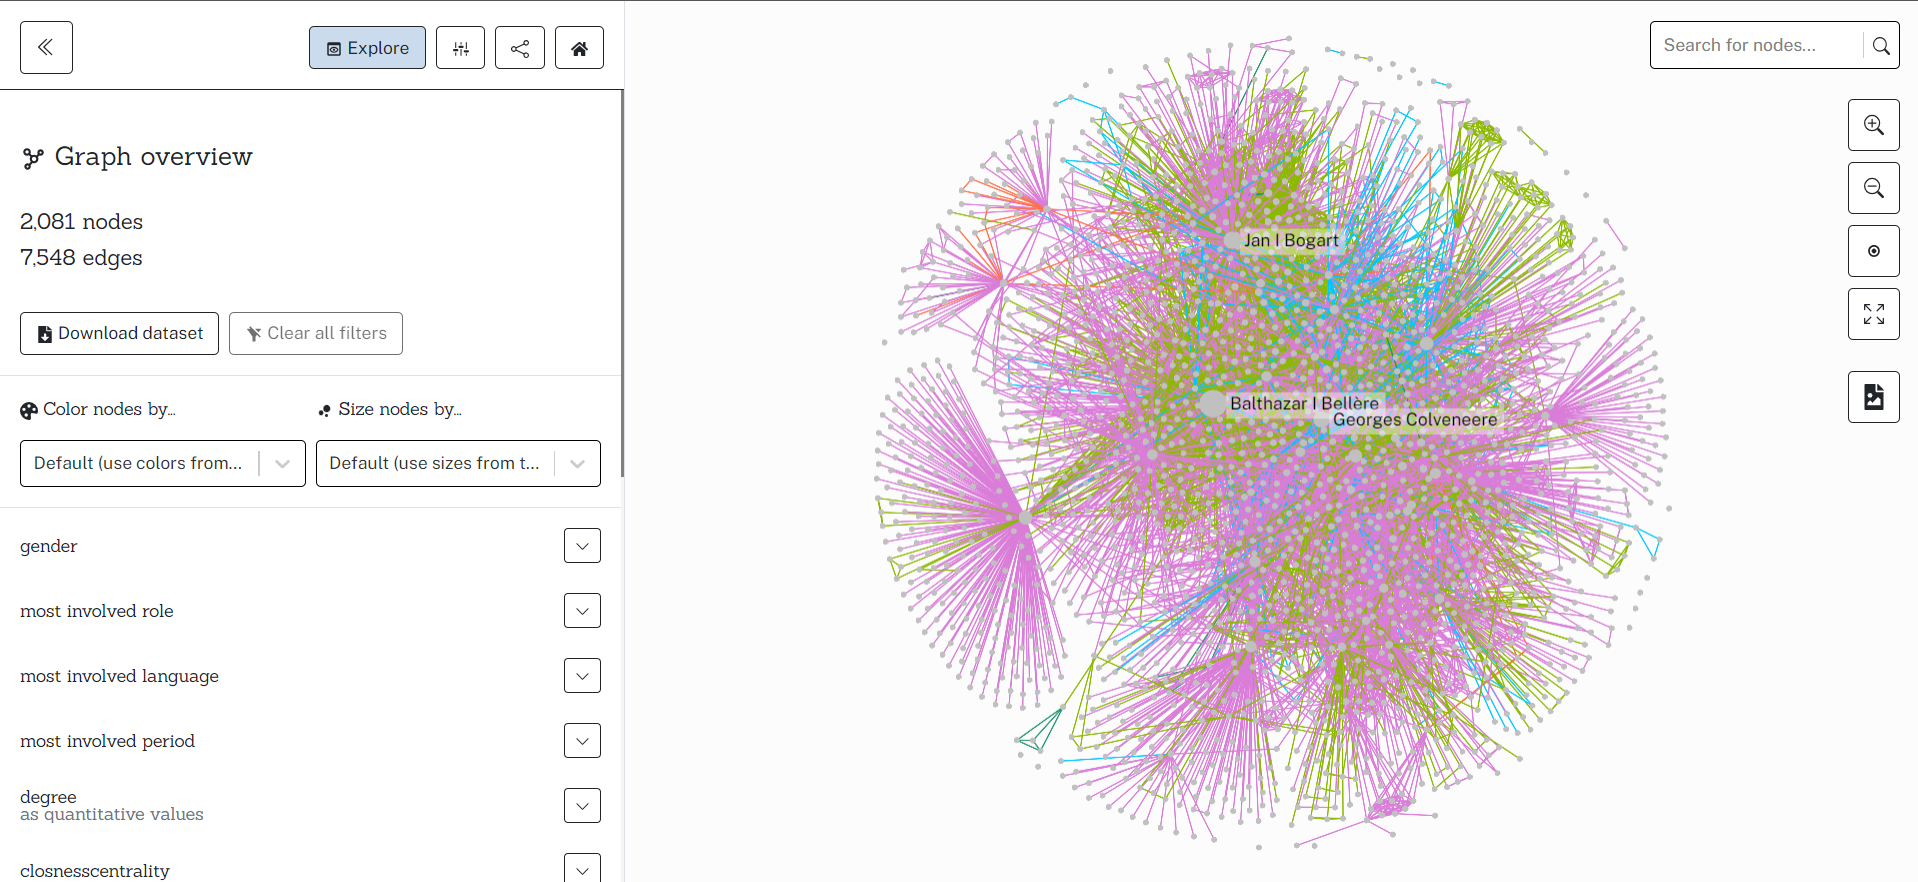
\includegraphics[scale=0.38]{graph/Retina-1.png}
\end{figure}

To the \href{https://ouestware.gitlab.io/retina/1.0.0-beta.1/#/graph/?url=https%3A%2F%2Fgist.githubusercontent.com%2Fdodopianist%2Feb21d80ea0e30d512a3c49d97f7e035a%2Fraw%2F993868d8a1aab1e07c3c7345e7b8dbb11b7c5edb%2Fcer_network.gexf&sa[]=ei&sa[]=be-n&sa[]=clo-n&sa[]=deg-n&ca[]=msr&ca[]=msl&ca[]=msp&ca[]=md-s&ca[]=pri&ca[]=hoo&ca[]=clu-n&ca[]=be-n&ca[]=clo-n&ca[]=deg-n&ca[]=bir&ca[]=dear&ca[]=deap&ca[]=ei&fa=bip&ec=o}{\underline{Compiler/Editor/Revisor Network}}.
\begin{figure}[H]
\centering
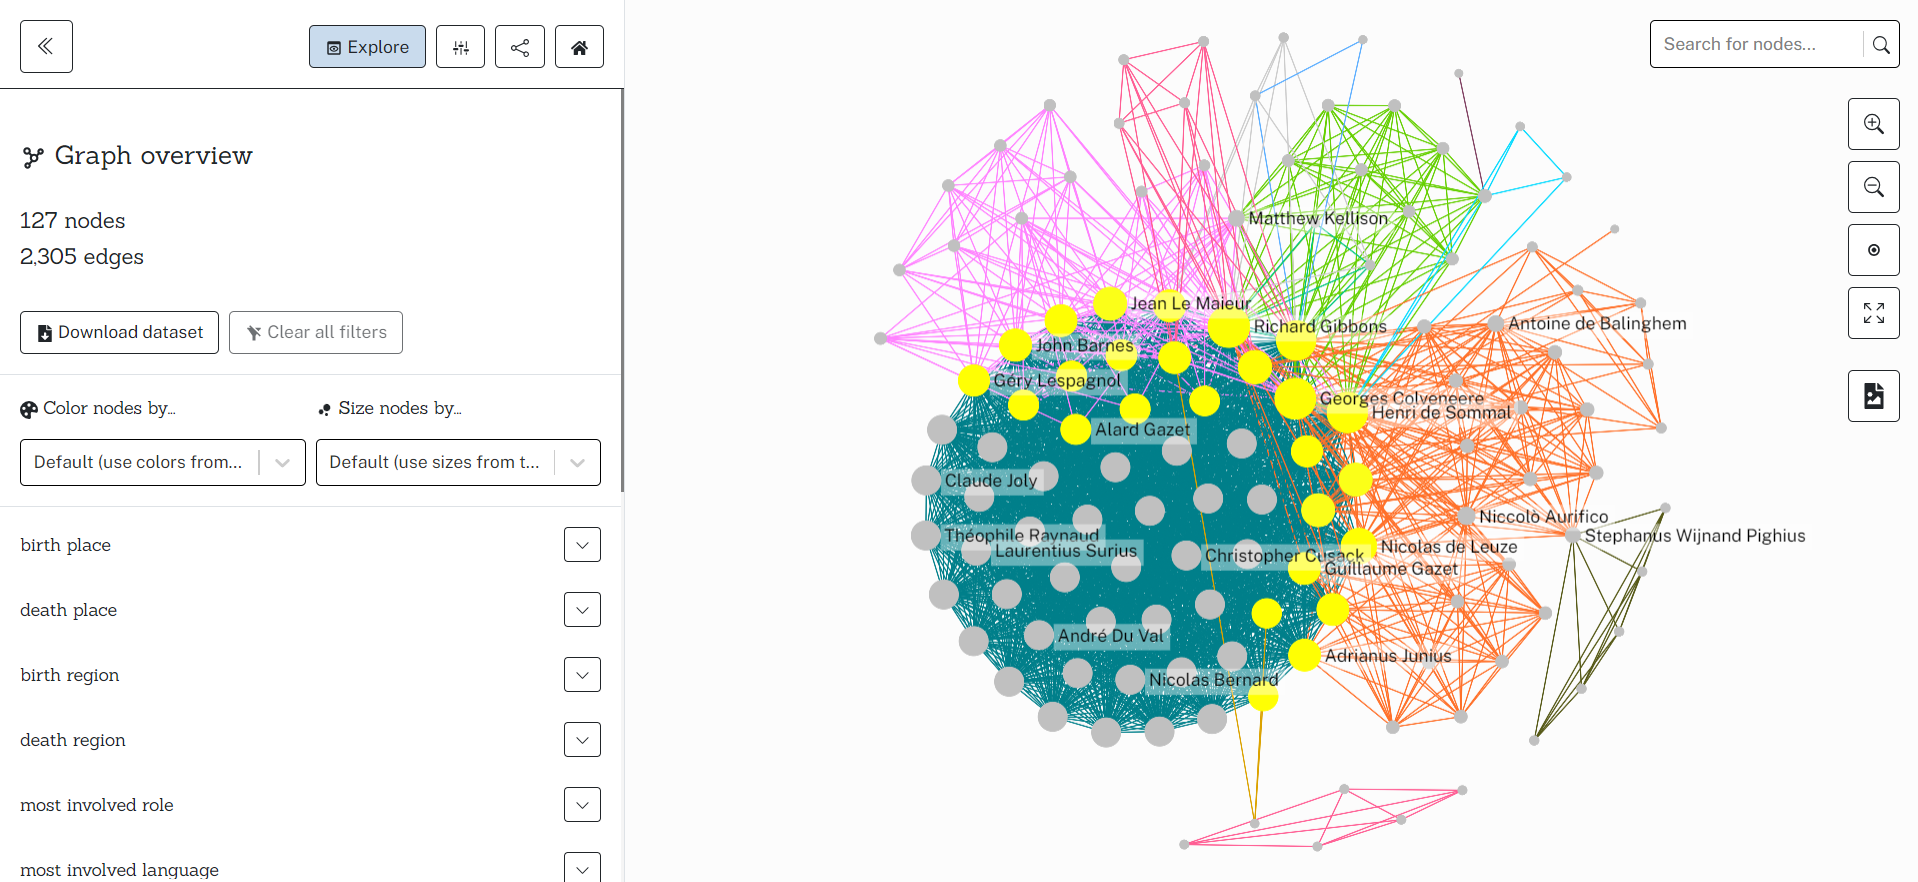
\includegraphics[scale=0.38]{graph/Retina-2.png}
\end{figure}

\counterwithout{footnote}{chapter}
\chapter{Conclusion}
\label{conclusion}
This paper examines the feasibility of Social Network Analysis on historical databases. Specifically, it analyses the “Duacensia” dataset, which records religious books published in Douai. The dataset is preprocessed before further analysis, including eliminating publications published outside the best ages (1559-1659) of the Douai publishing industry and making the formats of data to be more consistent. In addition, additional adjustments are applied to fix issues, such as the countries recorded in the dataset are not historically correct, and the information on the languages of publications is missing.

The most powerful and valuable aspect of Social Network Analysis when conducting it on historical databases can be its visualisation. Chapter \ref{comeAndGo} exhibits this visual ability. Historians already have an observation of the migration of English Catholics, and projecting people’s birth places and death places as a Network on the map can provide a clearer illustration of this mobility. Furthermore, Chapter \ref{differentNetwork} suggests that the diverse ways to plot the Networks can provide interesting insights. Section \ref{differentNetwork}.1 deploys the colour of nodes to highlight the shifting strategies of Kellam’s printing house and Section \ref{differentNetwork}.2 displays the long-term collaboration of printing houses with certain compilers/editors/revisors by just a single Network graph.

Metrics of Social Network Analysis can also offer rich information underlying a Network. In Chapter \ref{languages}, A line graph only shows the rise and decline of the Douai publishing industry correlated with the trend of Latin publications. However, Social Network Analysis reveals that the industry's development was initiated by the activities of English Catholics. Metrics of the People Network not only demonstrate the influence of English Catholics but also provide evidence of their deeper interactions with local experts and other communities, which contributed to the rise of the industry. In addition, with metrics of Social Network Analysis, Section \ref{influencers}.2 presents the participation and contribution of women to the industry.

Nevertheless, unlike modern databases, due to age, some information in historical databases may no longer be available. For example, in our research dataset, there are only 20\% of records of people’s birth and death places. Although we can use the languages of publication as a proxy to represent the dynamic of English Catholics in the Network, other historical databases may not be able to provide this type of proxy.

In conclusion, Social Network Analysis can help quantify historical databases and provide reliable evidence as a supplement to historians’ qualitative assumptions and observations. However, the potential of absent information in historical databases should be considered before conducting the analysis.

\nocite{*}
\printbibliography[
    heading=bibintoc,
    title={Reference}
]

\appendix
\chapter{Details of Grouping Roles}
\label{app:groupRoles}
\begin{longtable}{>{\hspace{0pt}}m{0.385\linewidth}|>{\hspace{0pt}}m{0.558\linewidth}}
\multicolumn{1}{>{\centering\hspace{0pt}}m{0.385\linewidth}}{\textbf{Role}} & \multicolumn{1}{>{\centering\arraybackslash\hspace{0pt}}m{0.558\linewidth}}{\textbf{Macro Role}}                                          \endfirsthead 
\hline
approbator                                                                  & approbator                                                                                                                                                   \\
\multicolumn{2}{>{\hspace{0pt}}m{0.943\linewidth}}{Who approved the publication.}                                                                                                                                                          \\ 
\hline
archbishop                                                                  & archbishop/bishop                                                                                                                                            \\
bishop                                                                      &                                                                                                                                                              \\
\multicolumn{2}{>{\hspace{0pt}}m{0.943\linewidth}}{They were the clergy.}                                                                                                                                                                  \\ 
\hline
author                                                                      & author                                                                                                                                                       \\
poet                                                                        &                                                                                                                                                              \\
\multicolumn{2}{>{\hspace{0pt}}m{0.943\linewidth}}{5 people under the same work, ID “43702”, are marked as poets. Since they all contributed texts in the same work, they are categorised as authors.}                                     \\ 
\hline
collaborator                                                                & collaborator/contributor/signer                                                                                                                              \\
contributor                                                                 &                                                                                                                                                              \\
signer                                                                      &                                                                                                                                                              \\
\multicolumn{2}{>{\hspace{0pt}}m{0.943\linewidth}}{They contributed to the work in some way but are not specific. Signers are the ones who confirmed the publication before it was printed (Jones et al., 2019).}                          \\ 
\hline
commentator                                                                 & commentator/eulogist                                                                                                                                         \\
eulogist                                                                    &                                                                                                                                                              \\
\multicolumn{2}{>{\hspace{0pt}}m{0.943\linewidth}}{They wrote extra texts (comments or compliments) that were not originally in the publication.}                                                                                          \\ 
\hline
compiler                                                                    & compiler/editor/revisor                                                                                                                                      \\
editor                                                                      &                                                                                                                                                              \\
revisor                                                                     &                                                                                                                                                              \\
\multicolumn{2}{>{\hspace{0pt}}m{0.943\linewidth}}{They were the ones who made the book, since the authors may have dead when the book was published.}                                                                                     \\ 
\hline
dedicatee                                                                   & dedicatee                                                                                                                                                    \\
\multicolumn{2}{>{\hspace{0pt}}m{0.943\linewidth}}{Who the publication was dedicated to.}                                                                                                                                                  \\ 
\hline
engraver                                                                    & engraver/etcher/illustrator                                                                                                                                  \\
etcher                                                                      &                                                                                                                                                              \\
illustrator                                                                 &                                                                                                                                                              \\
\multicolumn{2}{>{\hspace{0pt}}m{0.943\linewidth}}{They oversaw the art part (i.e., graphs) of the publication.}                                                                                                                           \\ 
\hline
heirs                                                                       & heirs/widow                                                                                                                                                  \\
widow                                                                       &                                                                                                                                                              \\
\multicolumn{2}{>{\hspace{0pt}}m{0.943\linewidth}}{They inherited the right to publish the publication.}                                                                                                                                   \\ 
\hline
bookseller                                                                  & printer/publisher                                                                                                                                            \\
printer                                                                     &                                                                                                                                                              \\
publisher                                                                   &                                                                                                                                                              \\
\multicolumn{2}{>{\hspace{0pt}}m{0.943\linewidth}}{Bookseller is categorised here since it also had a similar responsibility to a publisher (Jones et al., 2019), and there is only one person tagged as a bookseller in this dataset.}    \\
translator                                                                  & translator                                                                                                                                                   \\ 
\hline
information about in                                                        & unspecified                                                                                                                                                  \\
(blank)                                                                     &                                                                                                                                                             
\end{longtable}

\chapter{Details of Identified Printing Houses}
\label{app:printHouse}
\begin{longtable}{>{\hspace{0pt}}m{0.450\linewidth}>{\hspace{0pt}}m{0.170\linewidth}>{\hspace{0pt}}m{0.320\linewidth}}\\
\multicolumn{1}{>{\centering\hspace{0pt}}m{0.450\linewidth}}{\textbf{Printing House}} & \multicolumn{1}{>{\centering\hspace{0pt}}m{0.170\linewidth}}{\textbf{Origin}} & \multicolumn{1}{>{\centering\arraybackslash\hspace{0pt}}m{0.320\linewidth}}{\textbf{Member}}  \endfirsthead 
\hline
Auroy (Wyffels, 2017d)                                                                & Low Countries                                                                                                                     & André Auroy                                                                                                                           \\
                                                                                      &                                                                                                                                   & Dorothée Boscard                                                                                                                      \\
                                                                                      &                                                                                                                                   & Jacques Mairesse                                                                                                                      \\
                                                                                      &                                                                                                                                   & Pierre Auroy*                                                                                                                         \\
Bardou (Wyffels, 2017a)                                                               & Low Countries                                                                                                                     & Barthélémy Bardou*                                                                                                                    \\
Bellère (Wyffels, 2018f)                                                              & Low Countries                                                                                                                     & Anne de Behault                                                                                                                       \\
                                                                                      &                                                                                                                                   & Balthazar I Bellère*                                                                                                                  \\
                                                                                      &                                                                                                                                   & Balthazar II Bellere                                                                                                                  \\
                                                                                      &                                                                                                                                   & Pierre Bellere                                                                                                                        \\
Bogart (Wyffels, 2018d)                                                               & Low Countries                                                                                                                     & Denis Hutsebaut                                                                                                                       \\
                                                                                      &                                                                                                                                   & Françoise Pinchon                                                                                                                     \\
                                                                                      &                                                                                                                                   & Jan I Bogart*                                                                                                                         \\
                                                                                      &                                                                                                                                   & Jean II Bogart                                                                                                                        \\
                                                                                      &                                                                                                                                   & Martin Bogart                                                                                                                         \\
                                                                                      &                                                                                                                                   & Pierre Bogart                                                                                                                         \\
Borremans (Wyffels, 2017i)                                                            & Low Countries                                                                                                                     & Gertrud Heusch                                                                                                                        \\
                                                                                      &                                                                                                                                   & Pierre I Borremans*                                                                                                                   \\
                                                                                      &                                                                                                                                   & Pierre II Borremans                                                                                                                   \\
Boscard (Wyffels, 2017b)                                                              & Low Countries                                                                                                                     & Charles I Boscard                                                                                                                     \\
                                                                                      &                                                                                                                                   & Christine De Roovere                                                                                                                  \\
                                                                                      &                                                                                                                                   & Jacques Boscard*                                                                                                                      \\
Cnobbaert (Printing House of Jan I Cnobbaert, 2019)                                   & Low Countries                                                                                                                     & Jan I Cnobbaert*                                                                                                                      \\
de Fampoux (Wyffels, 2017n)                                                           & Low Countries                                                                                                                     & Jean de Fampoux*                                                                                                                      \\
de Spira (Wyffels, 2017f)                                                             & Low Countries                                                                                                                     & Jean de Spira*                                                                                                                        \\
de Winde (Wyffels, 2017g)                                                             & Low Countries                                                                                                                     & Lodewijk De Winde*                                                                                                                    \\
                                                                                      &                                                                                                                                   & Widow Lodewijk De Winde                                                                                                               \\
Diestre (Wyffels, 2017k)                                                              & Low Countries                                                                                                                     & Jean Diestre*                                                                                                                         \\
Duhamel (Wyffels, 2018b)                                                              & Low Countries                                                                                                                     & Joseph Duhamel*                                                                                                                       \\
English College Press (Soetaert, 2018b)                                               & Britain                                                                                                                           & John Heigham                                                                                                                          \\
                                                                                      &                                                                                                                                   & Robert Persons*                                                                                                                       \\
Fabri (Wyffels, 2017e)                                                                & Low Countries                                                                                                                     & François Fabri*                                                                                                                       \\
Fowler (Wyffels, 2017l)                                                               & Britain                                                                                                                           & John Fowler*                                                                                                                          \\
Galle (Printing House of Philips Galle, 2019)                                         & Low Countries                                                                                                                     & Theodoor Galle                                                                                                                        \\
Taylor (Wyffels, 2017o)                                                               & Britain                                                                                                                           & Henry Taylor*                                                                                                                         \\
Kellam (Wyffels, 2017m)                                                               & Britain                                                                                                                           & Laurence I Kellam*                                                                                                                    \\
                                                                                      &                                                                                                                                   & Laurence II Kellam                                                                                                                    \\
                                                                                      &                                                                                                                                   & Marguerite Lanseart                                                                                                                   \\
                                                                                      &                                                                                                                                   & Thomas (I) Kellam                                                                                                                     \\
Nutius (Wyffels, 2019b)                                                               & Low Countries                                                                                                                     & Marie Borrewater                                                                                                                      \\
                                                                                      &                                                                                                                                   & Martinus I Nutius*                                                                                                                    \\
                                                                                      &                                                                                                                                   & Martinus II Nutius                                                                                                                    \\
                                                                                      &                                                                                                                                   & Philippus Nutius                                                                                                                      \\
Pinchon (Wyffels, 2018a)                                                              & Low Countries                                                                                                                     & Gérard Pinchon*                                                                                                                       \\
Plantin (Wyffels, 2020)                                                               & Low Countries                                                                                                                     & Christophe Plantin*                                                                                                                   \\
                                                                                      &                                                                                                                                   & Frans Raphelengius                                                                                                                    \\
Serrurier (Wyffels, 2017c)                                                            & Low Countries                                                                                                                     & Jean Serrurier*                                                                                                                       \\
                                                                                      &                                                                                                                                   & Marie Marquette                                                                                                                       \\
Sleghers (Wyffels, 2019d)                                                             & Low Countries                                                                                                                     & Reynier Sleghers*                                                                                                                     \\
Usselinx (Wyffels, 2017j)                                                             & Low Countries                                                                                                                     & Henri Usselinx*                                                                                                                       \\
van Wolsschaten (Wyffels, 2019c)                                                      & Low Countries                                                                                                                     & Gerard I van Wolsschaten*                                                                                                             \\
Velpius (Wyffels, 2018e)                                                              & Low Countries                                                                                                                     & Reinerus II Velpius                                                                                                                   \\
Verdussen (Wyffels, 2019a)                                                            & Low Countries                                                                                                                     & Hieronymus I Verdussen*                                                                                                               \\
Wardavoir (Wyffels, 2017h)                                                            & Low Countries                                                                                                                     & Jean Patte                                                                                                                            \\
                                                                                      &                                                                                                                                   & Jeanne de Menin                                                                                                                       \\
                                                                                      &                                                                                                                                   & Nicolas Telu                                                                                                                          \\
                                                                                      &                                                                                                                                   & Noël Wardavoir*                                                                                                                       \\
                                                                                      &                                                                                                                                   & Pierre Telu                                                                                                                           \\
Wyon (Wyffels, 2018c)                                                                 & Low Countries                                                                                                                     & Marc Wyon*                                                                                                                            \\
                                                                                      &                                                                                                                                   & Marie Vanderpiet                                                                                                                     
\end{longtable}

\end{sloppypar}
\newpage
% ----------------------- Back cover ------------------------------
% Please fill in:
% - Department
% - Department's address
% - Telephone number and fax number
% -----------------------------------------------------------------
\thispagestyle{empty}
\sffamily
%
\begin{textblock}{191}(106,-11)
{\color{blueline}\rule{178pt}{5.5pt}}
\end{textblock}
%
\begin{textblock}{191}(168,-11)
{\color{blueline}\rule{5.5pt}{61pt}}
\end{textblock}
%
\begin{textblock}{183}(-24,-11)
\textblockcolour{}
\flushright
\fontsize{7}{7.5}\selectfont
\textbf{Departement Computerwetenschappen}\\
Celestijnenlaan 200A - bus 2402\\
3001 LEUVEN, BELGI\"{E}\\
tel. + 32 16 32 77 00\\
fax + 32 16 32 79 96\\
wms.cs.kuleuven.be\\
\end{textblock}
%
\begin{textblock}{191}(155,-7)
\textblockcolour{}
\includegraphics*[height=16.5truemm]{sedes}
\end{textblock}
%
\begin{textblock}{191}(-20,235)
{\color{bluetitle}\rule{544pt}{55pt}}
\end{textblock}
\end{document}